\documentclass[]{article}
\usepackage{lmodern}
\usepackage{amssymb,amsmath}
\usepackage{ifxetex,ifluatex}
\usepackage{fixltx2e} % provides \textsubscript
\ifnum 0\ifxetex 1\fi\ifluatex 1\fi=0 % if pdftex
  \usepackage[T1]{fontenc}
  \usepackage[utf8]{inputenc}
\else % if luatex or xelatex
  \ifxetex
    \usepackage{mathspec}
  \else
    \usepackage{fontspec}
  \fi
  \defaultfontfeatures{Ligatures=TeX,Scale=MatchLowercase}
\fi
% use upquote if available, for straight quotes in verbatim environments
\IfFileExists{upquote.sty}{\usepackage{upquote}}{}
% use microtype if available
\IfFileExists{microtype.sty}{%
\usepackage{microtype}
\UseMicrotypeSet[protrusion]{basicmath} % disable protrusion for tt fonts
}{}
\usepackage[margin=1in]{geometry}
\usepackage{hyperref}
\hypersetup{unicode=true,
            pdftitle={Unofficial Solutions to R for Data Science},
            pdfauthor={Lok H. Chau},
            pdfborder={0 0 0},
            breaklinks=true}
\urlstyle{same}  % don't use monospace font for urls
\usepackage{natbib}
\bibliographystyle{plainnat}
\usepackage{color}
\usepackage{fancyvrb}
\newcommand{\VerbBar}{|}
\newcommand{\VERB}{\Verb[commandchars=\\\{\}]}
\DefineVerbatimEnvironment{Highlighting}{Verbatim}{commandchars=\\\{\}}
% Add ',fontsize=\small' for more characters per line
\usepackage{framed}
\definecolor{shadecolor}{RGB}{248,248,248}
\newenvironment{Shaded}{\begin{snugshade}}{\end{snugshade}}
\newcommand{\KeywordTok}[1]{\textcolor[rgb]{0.13,0.29,0.53}{\textbf{#1}}}
\newcommand{\DataTypeTok}[1]{\textcolor[rgb]{0.13,0.29,0.53}{#1}}
\newcommand{\DecValTok}[1]{\textcolor[rgb]{0.00,0.00,0.81}{#1}}
\newcommand{\BaseNTok}[1]{\textcolor[rgb]{0.00,0.00,0.81}{#1}}
\newcommand{\FloatTok}[1]{\textcolor[rgb]{0.00,0.00,0.81}{#1}}
\newcommand{\ConstantTok}[1]{\textcolor[rgb]{0.00,0.00,0.00}{#1}}
\newcommand{\CharTok}[1]{\textcolor[rgb]{0.31,0.60,0.02}{#1}}
\newcommand{\SpecialCharTok}[1]{\textcolor[rgb]{0.00,0.00,0.00}{#1}}
\newcommand{\StringTok}[1]{\textcolor[rgb]{0.31,0.60,0.02}{#1}}
\newcommand{\VerbatimStringTok}[1]{\textcolor[rgb]{0.31,0.60,0.02}{#1}}
\newcommand{\SpecialStringTok}[1]{\textcolor[rgb]{0.31,0.60,0.02}{#1}}
\newcommand{\ImportTok}[1]{#1}
\newcommand{\CommentTok}[1]{\textcolor[rgb]{0.56,0.35,0.01}{\textit{#1}}}
\newcommand{\DocumentationTok}[1]{\textcolor[rgb]{0.56,0.35,0.01}{\textbf{\textit{#1}}}}
\newcommand{\AnnotationTok}[1]{\textcolor[rgb]{0.56,0.35,0.01}{\textbf{\textit{#1}}}}
\newcommand{\CommentVarTok}[1]{\textcolor[rgb]{0.56,0.35,0.01}{\textbf{\textit{#1}}}}
\newcommand{\OtherTok}[1]{\textcolor[rgb]{0.56,0.35,0.01}{#1}}
\newcommand{\FunctionTok}[1]{\textcolor[rgb]{0.00,0.00,0.00}{#1}}
\newcommand{\VariableTok}[1]{\textcolor[rgb]{0.00,0.00,0.00}{#1}}
\newcommand{\ControlFlowTok}[1]{\textcolor[rgb]{0.13,0.29,0.53}{\textbf{#1}}}
\newcommand{\OperatorTok}[1]{\textcolor[rgb]{0.81,0.36,0.00}{\textbf{#1}}}
\newcommand{\BuiltInTok}[1]{#1}
\newcommand{\ExtensionTok}[1]{#1}
\newcommand{\PreprocessorTok}[1]{\textcolor[rgb]{0.56,0.35,0.01}{\textit{#1}}}
\newcommand{\AttributeTok}[1]{\textcolor[rgb]{0.77,0.63,0.00}{#1}}
\newcommand{\RegionMarkerTok}[1]{#1}
\newcommand{\InformationTok}[1]{\textcolor[rgb]{0.56,0.35,0.01}{\textbf{\textit{#1}}}}
\newcommand{\WarningTok}[1]{\textcolor[rgb]{0.56,0.35,0.01}{\textbf{\textit{#1}}}}
\newcommand{\AlertTok}[1]{\textcolor[rgb]{0.94,0.16,0.16}{#1}}
\newcommand{\ErrorTok}[1]{\textcolor[rgb]{0.64,0.00,0.00}{\textbf{#1}}}
\newcommand{\NormalTok}[1]{#1}
\usepackage{longtable,booktabs}
\usepackage{graphicx,grffile}
\makeatletter
\def\maxwidth{\ifdim\Gin@nat@width>\linewidth\linewidth\else\Gin@nat@width\fi}
\def\maxheight{\ifdim\Gin@nat@height>\textheight\textheight\else\Gin@nat@height\fi}
\makeatother
% Scale images if necessary, so that they will not overflow the page
% margins by default, and it is still possible to overwrite the defaults
% using explicit options in \includegraphics[width, height, ...]{}
\setkeys{Gin}{width=\maxwidth,height=\maxheight,keepaspectratio}
\IfFileExists{parskip.sty}{%
\usepackage{parskip}
}{% else
\setlength{\parindent}{0pt}
\setlength{\parskip}{6pt plus 2pt minus 1pt}
}
\setlength{\emergencystretch}{3em}  % prevent overfull lines
\providecommand{\tightlist}{%
  \setlength{\itemsep}{0pt}\setlength{\parskip}{0pt}}
\setcounter{secnumdepth}{5}
% Redefines (sub)paragraphs to behave more like sections
\ifx\paragraph\undefined\else
\let\oldparagraph\paragraph
\renewcommand{\paragraph}[1]{\oldparagraph{#1}\mbox{}}
\fi
\ifx\subparagraph\undefined\else
\let\oldsubparagraph\subparagraph
\renewcommand{\subparagraph}[1]{\oldsubparagraph{#1}\mbox{}}
\fi

%%% Use protect on footnotes to avoid problems with footnotes in titles
\let\rmarkdownfootnote\footnote%
\def\footnote{\protect\rmarkdownfootnote}

%%% Change title format to be more compact
\usepackage{titling}

% Create subtitle command for use in maketitle
\newcommand{\subtitle}[1]{
  \posttitle{
    \begin{center}\large#1\end{center}
    }
}

\setlength{\droptitle}{-2em}
  \title{Unofficial Solutions to R for Data Science}
  \pretitle{\vspace{\droptitle}\centering\huge}
  \posttitle{\par}
  \author{Lok H. Chau}
  \preauthor{\centering\large\emph}
  \postauthor{\par}
  \date{}
  \predate{}\postdate{}

\usepackage{booktabs}

\usepackage{amsthm}
\newtheorem{theorem}{Theorem}[section]
\newtheorem{lemma}{Lemma}[section]
\theoremstyle{definition}
\newtheorem{definition}{Definition}[section]
\newtheorem{corollary}{Corollary}[section]
\newtheorem{proposition}{Proposition}[section]
\theoremstyle{definition}
\newtheorem{example}{Example}[section]
\theoremstyle{definition}
\newtheorem{exercise}{Exercise}[section]
\theoremstyle{remark}
\newtheorem*{remark}{Remark}
\newtheorem*{solution}{Solution}
\begin{document}
\maketitle

{
\setcounter{tocdepth}{2}
\tableofcontents
}
\section*{About}\label{about}
\addcontentsline{toc}{section}{About}

\section{Introduction}\label{introduction}

No exercises.

\part{Explore}\label{part-explore}

\section{Introduction}\label{introduction-1}

No exercises.

\section{Data visualization}\label{data-visualization}

\subsection{Introduction}\label{introduction-2}

No exercises.

\subsection{First steps}\label{first-steps}

\subsubsection{Exercises}\label{exercises}

\emph{1 - Run \texttt{ggplot(data\ =\ mpg)}. What do you see?}

\begin{Shaded}
\begin{Highlighting}[]
\KeywordTok{ggplot}\NormalTok{(}\DataTypeTok{data =}\NormalTok{ mpg)}
\end{Highlighting}
\end{Shaded}


\includegraphics{R4DS_bookdown_files/figure-latex/unnamed-chunk-2-1.pdf}

In this case, nothing is displayed because we have specified neither the
mapping and geom.

\emph{2 - How many rows are in \texttt{mpg}? How many columns?}

To get the dimensions of a data matrix, we can simply use the function
`dim()'.

\begin{Shaded}
\begin{Highlighting}[]
\KeywordTok{dim}\NormalTok{(mpg)}
\end{Highlighting}
\end{Shaded}

\begin{verbatim}
## [1] 234  11
\end{verbatim}

The function returns a vector of values. The first element is the number
of rows and the second element is the number of columns. For mpg, we
have 234 rows and 11 columns.

Alternatively, we can use `nrow()' and'ncol()' to return the number of
rows and columns respectively.

\begin{Shaded}
\begin{Highlighting}[]
\KeywordTok{nrow}\NormalTok{(mpg)}
\end{Highlighting}
\end{Shaded}

\begin{verbatim}
## [1] 234
\end{verbatim}

\begin{Shaded}
\begin{Highlighting}[]
\KeywordTok{ncol}\NormalTok{(mpg)}
\end{Highlighting}
\end{Shaded}

\begin{verbatim}
## [1] 11
\end{verbatim}

\emph{3 - What does the \texttt{drv} variable describe? Read the help
for \texttt{?mpg} to find out.}

f = front-wheel drive r = rear wheel drive 4 = 4wd

\emph{4 -Make a scatterplot of \texttt{hwy} vs \texttt{cyl}.}

\begin{Shaded}
\begin{Highlighting}[]
\KeywordTok{ggplot}\NormalTok{(}\DataTypeTok{data =}\NormalTok{ mpg) }\OperatorTok{+}
\StringTok{  }\KeywordTok{geom_point}\NormalTok{(}\DataTypeTok{mapping =} \KeywordTok{aes}\NormalTok{(}\DataTypeTok{x =}\NormalTok{ cyl, }\DataTypeTok{y =}\NormalTok{ hwy))}
\end{Highlighting}
\end{Shaded}

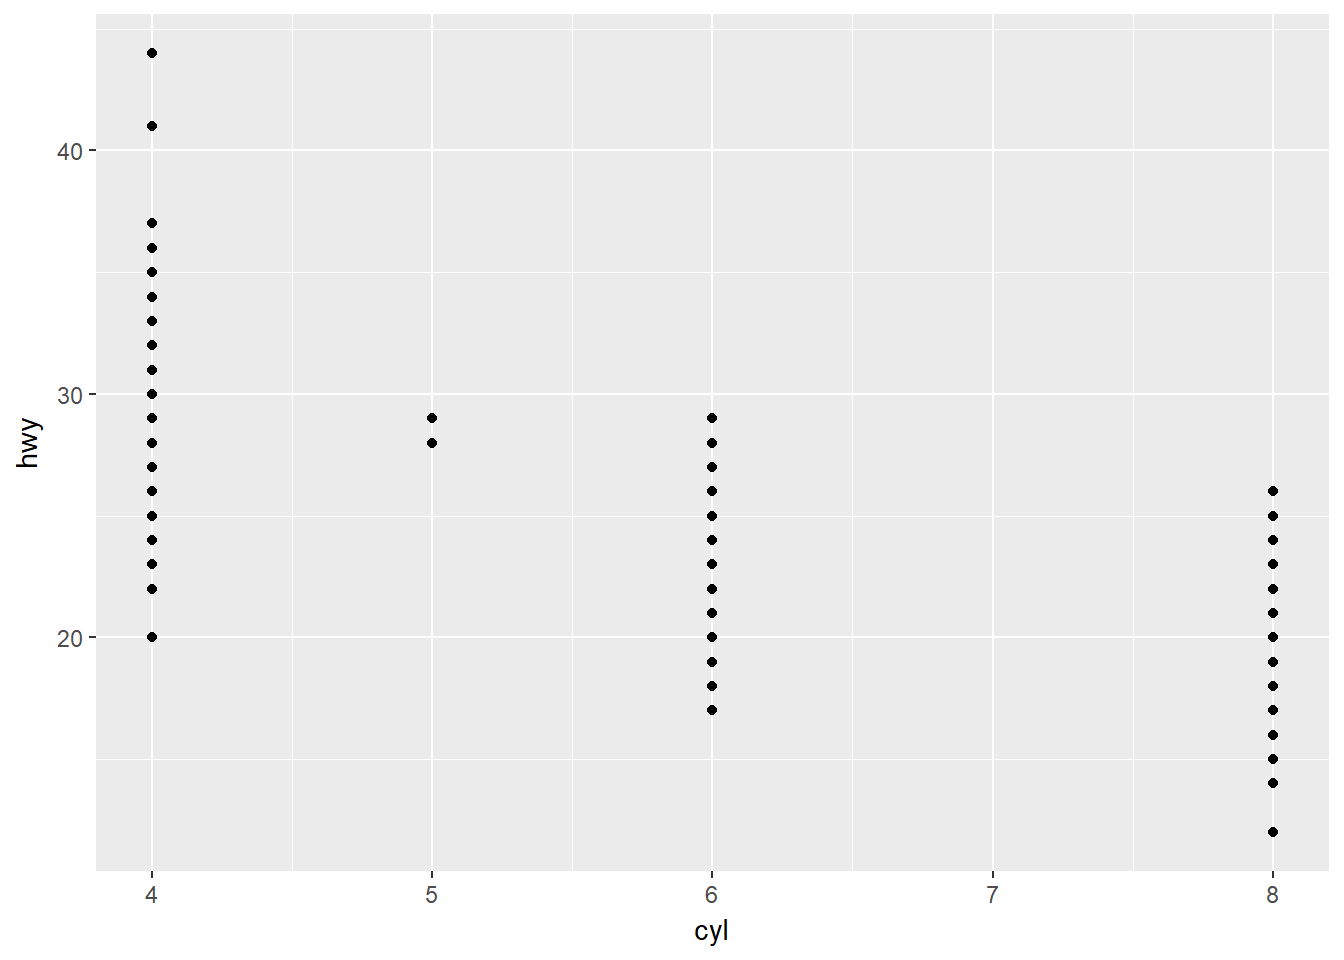
\includegraphics{R4DS_bookdown_files/figure-latex/unnamed-chunk-6-1.pdf}

\emph{5 - What happens if you make a scatterplot of \texttt{class} vs
\texttt{drv}? Why is the plot not useful?}

\begin{Shaded}
\begin{Highlighting}[]
\KeywordTok{ggplot}\NormalTok{(}\DataTypeTok{data =}\NormalTok{ mpg) }\OperatorTok{+}
\StringTok{  }\KeywordTok{geom_point}\NormalTok{(}\DataTypeTok{mapping =} \KeywordTok{aes}\NormalTok{(}\DataTypeTok{x =}\NormalTok{ drv, }\DataTypeTok{y =}\NormalTok{ class))}
\end{Highlighting}
\end{Shaded}

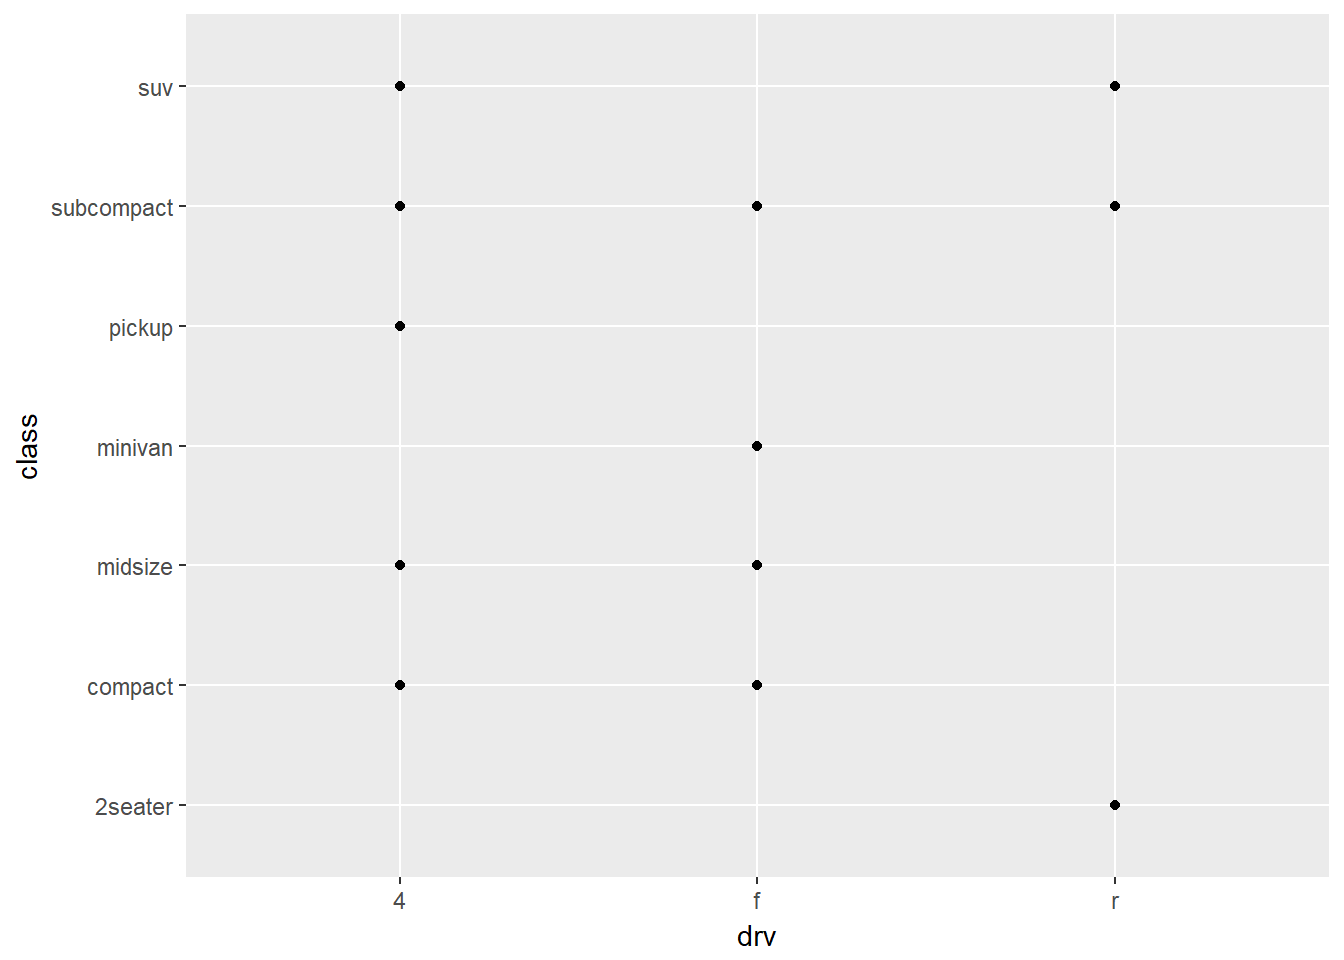
\includegraphics{R4DS_bookdown_files/figure-latex/unnamed-chunk-7-1.pdf}

In this dataset, both \texttt{class} and \texttt{drv} are categorical
variables. The only information this scatter plot reveals is what
combinations of class and drv exist in the dataset. For example, there
are front-wheel drive compact vehicles, but not front-wheel drive 2
seaters.

\subsection{Aesthetic mappings}\label{aesthetic-mappings}

\subsubsection{Exercises}\label{exercises-1}

\emph{1 - What's gone wrong with this code? Why are the points not
blue?}

\begin{Shaded}
\begin{Highlighting}[]
\KeywordTok{ggplot}\NormalTok{(}\DataTypeTok{data =}\NormalTok{ mpg) }\OperatorTok{+}\StringTok{ }
\StringTok{  }\KeywordTok{geom_point}\NormalTok{(}\DataTypeTok{mapping =} \KeywordTok{aes}\NormalTok{(}\DataTypeTok{x =}\NormalTok{ displ, }\DataTypeTok{y =}\NormalTok{ hwy, }\DataTypeTok{color =} \StringTok{"blue"}\NormalTok{))}
\end{Highlighting}
\end{Shaded}

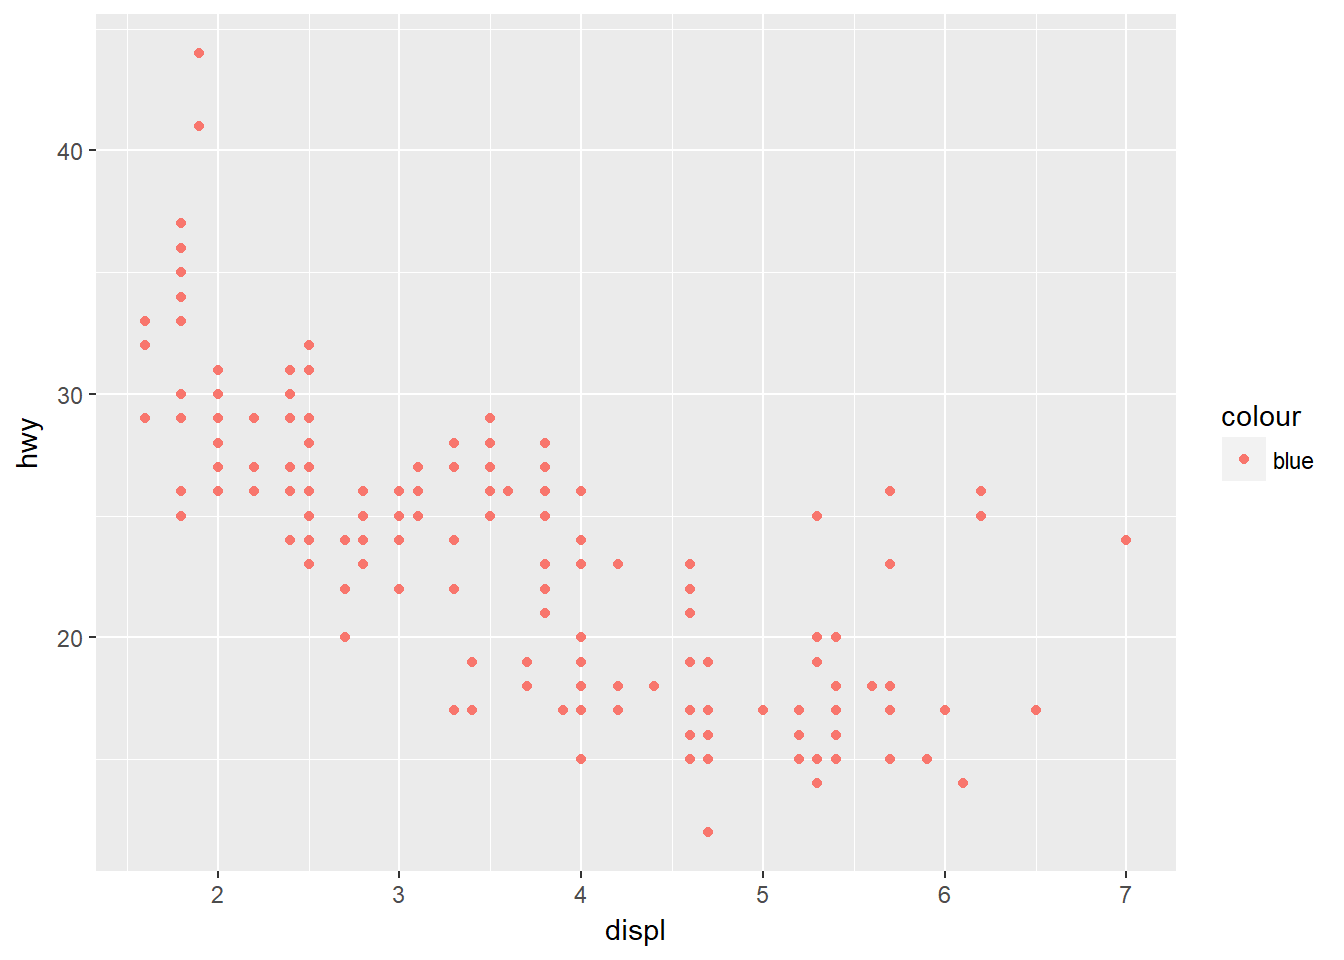
\includegraphics{R4DS_bookdown_files/figure-latex/unnamed-chunk-8-1.pdf}

In order to manually change the color of every point to blue,
\texttt{color\ =\ "blue"} should be placed outside the \texttt{aes()}
argument.

\begin{Shaded}
\begin{Highlighting}[]
\KeywordTok{ggplot}\NormalTok{(}\DataTypeTok{data =}\NormalTok{ mpg) }\OperatorTok{+}\StringTok{ }
\StringTok{  }\KeywordTok{geom_point}\NormalTok{(}\DataTypeTok{mapping =} \KeywordTok{aes}\NormalTok{(}\DataTypeTok{x =}\NormalTok{ displ, }\DataTypeTok{y =}\NormalTok{ hwy), }\DataTypeTok{color =} \StringTok{"blue"}\NormalTok{)}
\end{Highlighting}
\end{Shaded}

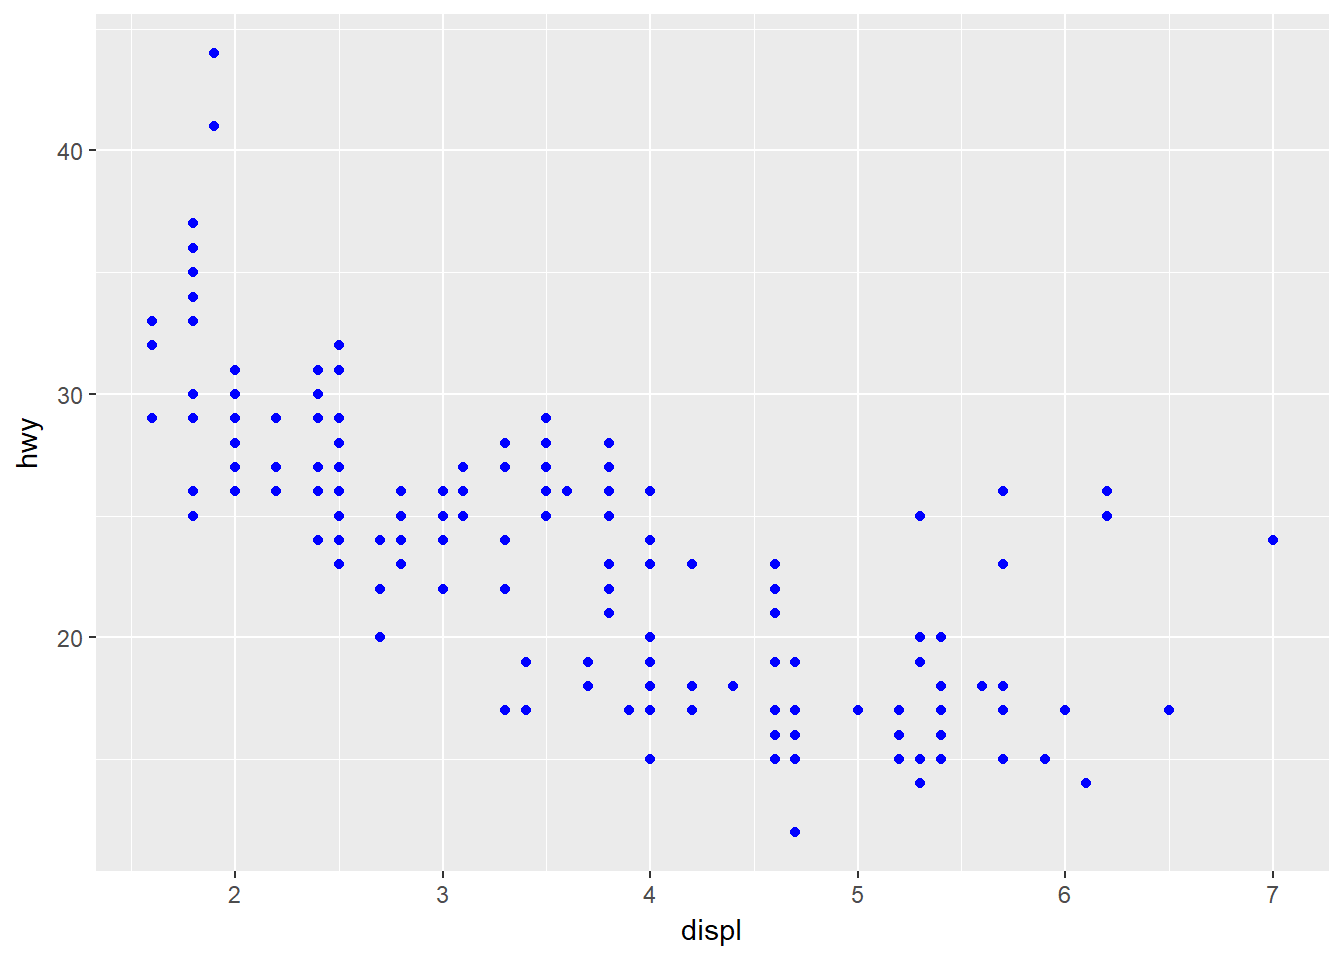
\includegraphics{R4DS_bookdown_files/figure-latex/unnamed-chunk-9-1.pdf}

\emph{2 - Which variables in \texttt{mpg} are categorical? Which
variables are continuous? (Hint: type \texttt{?mpg} to read the
documentation for the dataset). How can you see this information when
you run \texttt{mpg}?}

We can type \texttt{?mpg} and deduce which variables are categorical and
which are continuous based on the descriptions. Or we can use
\texttt{str()} to get the types of the variables.

\begin{Shaded}
\begin{Highlighting}[]
\KeywordTok{str}\NormalTok{(mpg)}
\end{Highlighting}
\end{Shaded}

\begin{verbatim}
## Classes 'tbl_df', 'tbl' and 'data.frame':    234 obs. of  11 variables:
##  $ manufacturer: chr  "audi" "audi" "audi" "audi" ...
##  $ model       : chr  "a4" "a4" "a4" "a4" ...
##  $ displ       : num  1.8 1.8 2 2 2.8 2.8 3.1 1.8 1.8 2 ...
##  $ year        : int  1999 1999 2008 2008 1999 1999 2008 1999 1999 2008 ...
##  $ cyl         : int  4 4 4 4 6 6 6 4 4 4 ...
##  $ trans       : chr  "auto(l5)" "manual(m5)" "manual(m6)" "auto(av)" ...
##  $ drv         : chr  "f" "f" "f" "f" ...
##  $ cty         : int  18 21 20 21 16 18 18 18 16 20 ...
##  $ hwy         : int  29 29 31 30 26 26 27 26 25 28 ...
##  $ fl          : chr  "p" "p" "p" "p" ...
##  $ class       : chr  "compact" "compact" "compact" "compact" ...
\end{verbatim}

\texttt{manufacturer}, \texttt{model}, \texttt{trans}, \texttt{drv},
\texttt{fl}, and \texttt{class} are \texttt{chr} variables, which also
mean that they are categorical variables.

\emph{3 - Map a continuous variable to \texttt{color}, \texttt{size},
and \texttt{shape}. How do these aesthetics behave differently for
categorical vs.~continuous variables?}

When mapping a continuous variable, \texttt{displ}, to \texttt{color},
ggplot creats a gradient color scale to represent the values of the
continous variable. By default, ggplot creates a color gradient scale
from light blue to dark blue, where light blue reresents lower values
and dark blue represents higher values.

\begin{Shaded}
\begin{Highlighting}[]
\KeywordTok{ggplot}\NormalTok{(}\DataTypeTok{data =}\NormalTok{ mpg) }\OperatorTok{+}
\StringTok{  }\KeywordTok{geom_point}\NormalTok{(}\DataTypeTok{mapping =} \KeywordTok{aes}\NormalTok{(}\DataTypeTok{x =}\NormalTok{ displ, }\DataTypeTok{y =}\NormalTok{ hwy, }\DataTypeTok{color =}\NormalTok{ displ))}
\end{Highlighting}
\end{Shaded}

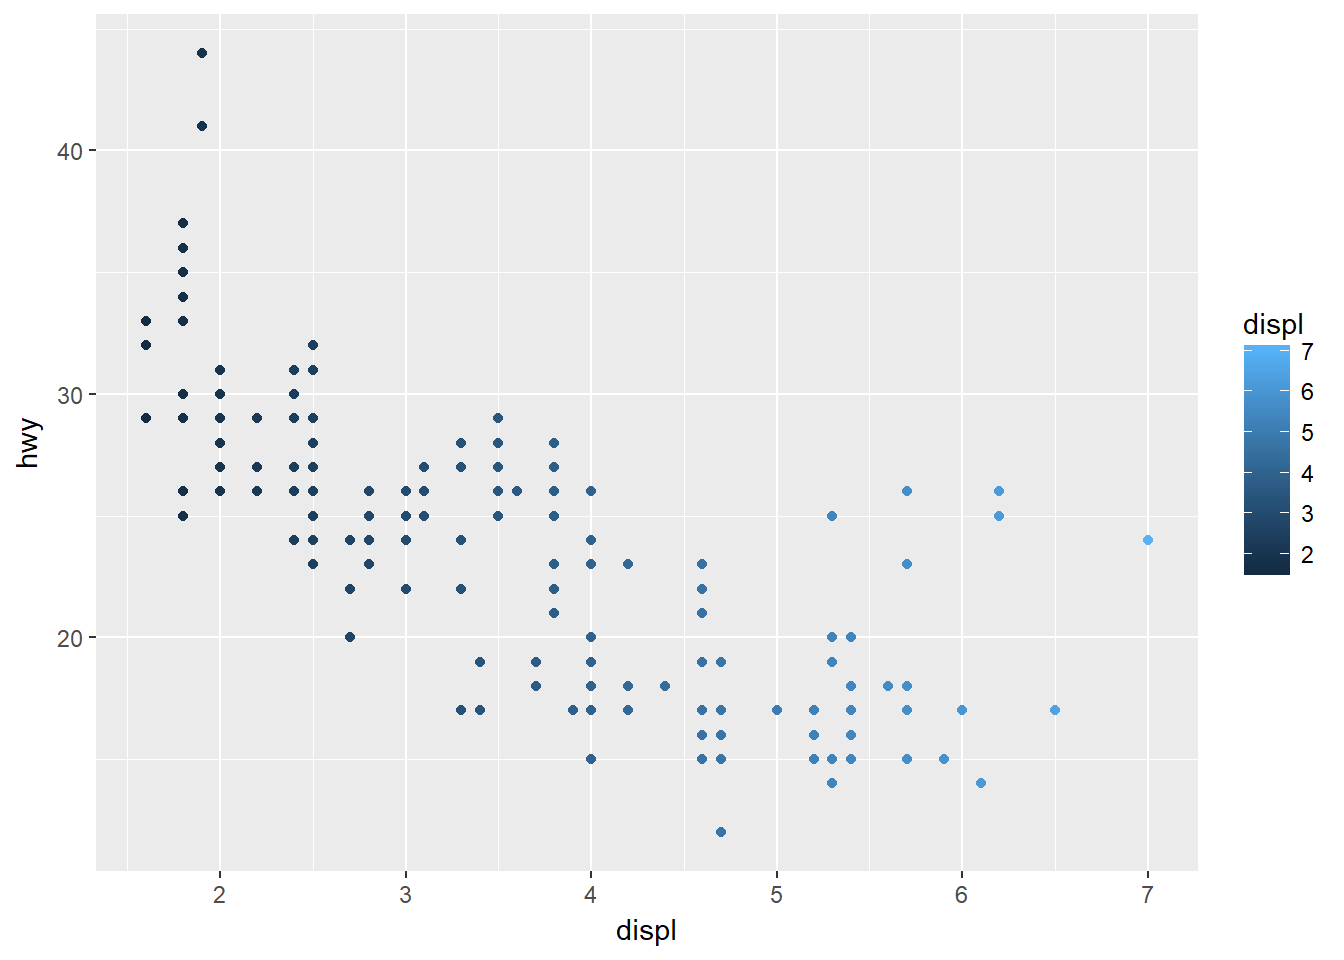
\includegraphics{R4DS_bookdown_files/figure-latex/unnamed-chunk-11-1.pdf}

Similiarly, when mapping a continuous variable to \texttt{shape}, ggplot
displays larger values with circles with larger area.

\begin{Shaded}
\begin{Highlighting}[]
\KeywordTok{ggplot}\NormalTok{(}\DataTypeTok{data =}\NormalTok{ mpg) }\OperatorTok{+}
\StringTok{  }\KeywordTok{geom_point}\NormalTok{(}\DataTypeTok{mapping =} \KeywordTok{aes}\NormalTok{(}\DataTypeTok{x =}\NormalTok{ displ, }\DataTypeTok{y =}\NormalTok{ hwy, }\DataTypeTok{size =}\NormalTok{ displ))}
\end{Highlighting}
\end{Shaded}

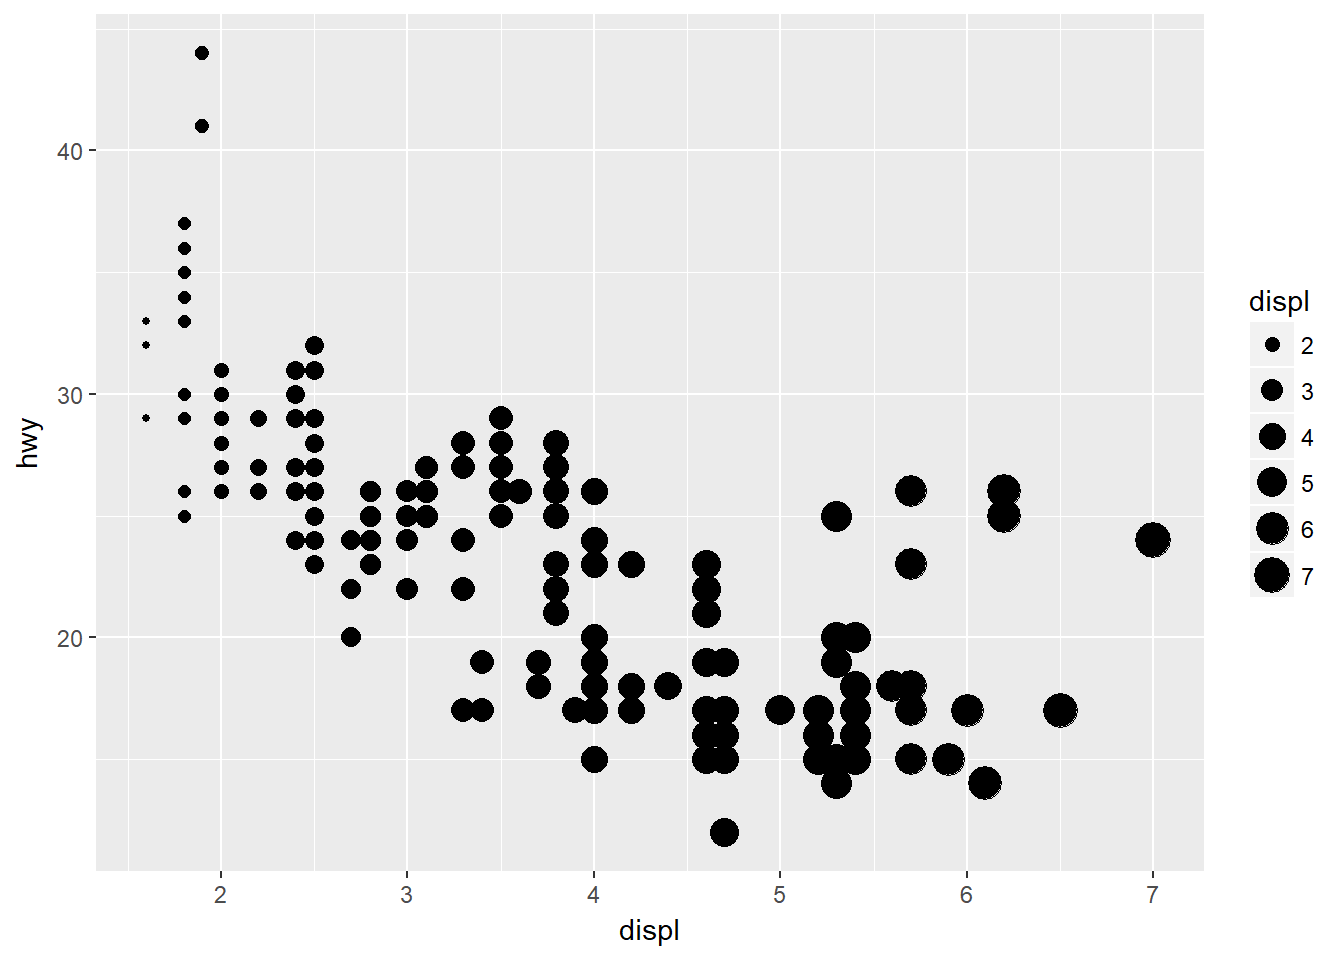
\includegraphics{R4DS_bookdown_files/figure-latex/unnamed-chunk-12-1.pdf}

However, ggplot with throw out an error message if we map a continuous
variable to \texttt{shape}.

\emph{4 - What happens if you map the same variable to multiple
aesthetics?}

We can map the same variable to multiple aesthetics, as long as the
aesethetics are compatiable with the type of the variables
(categorical/continuous). For example, we can map \texttt{drv}, which is
a categorical variable, to both \texttt{color} and \texttt{shape}.

\begin{Shaded}
\begin{Highlighting}[]
\KeywordTok{ggplot}\NormalTok{(}\DataTypeTok{data =}\NormalTok{ mpg) }\OperatorTok{+}
\StringTok{  }\KeywordTok{geom_point}\NormalTok{(}\DataTypeTok{mapping =} \KeywordTok{aes}\NormalTok{(}\DataTypeTok{x =}\NormalTok{ displ, }\DataTypeTok{y =}\NormalTok{ hwy, }\DataTypeTok{color =}\NormalTok{ drv, }\DataTypeTok{shape =}\NormalTok{ drv))}
\end{Highlighting}
\end{Shaded}

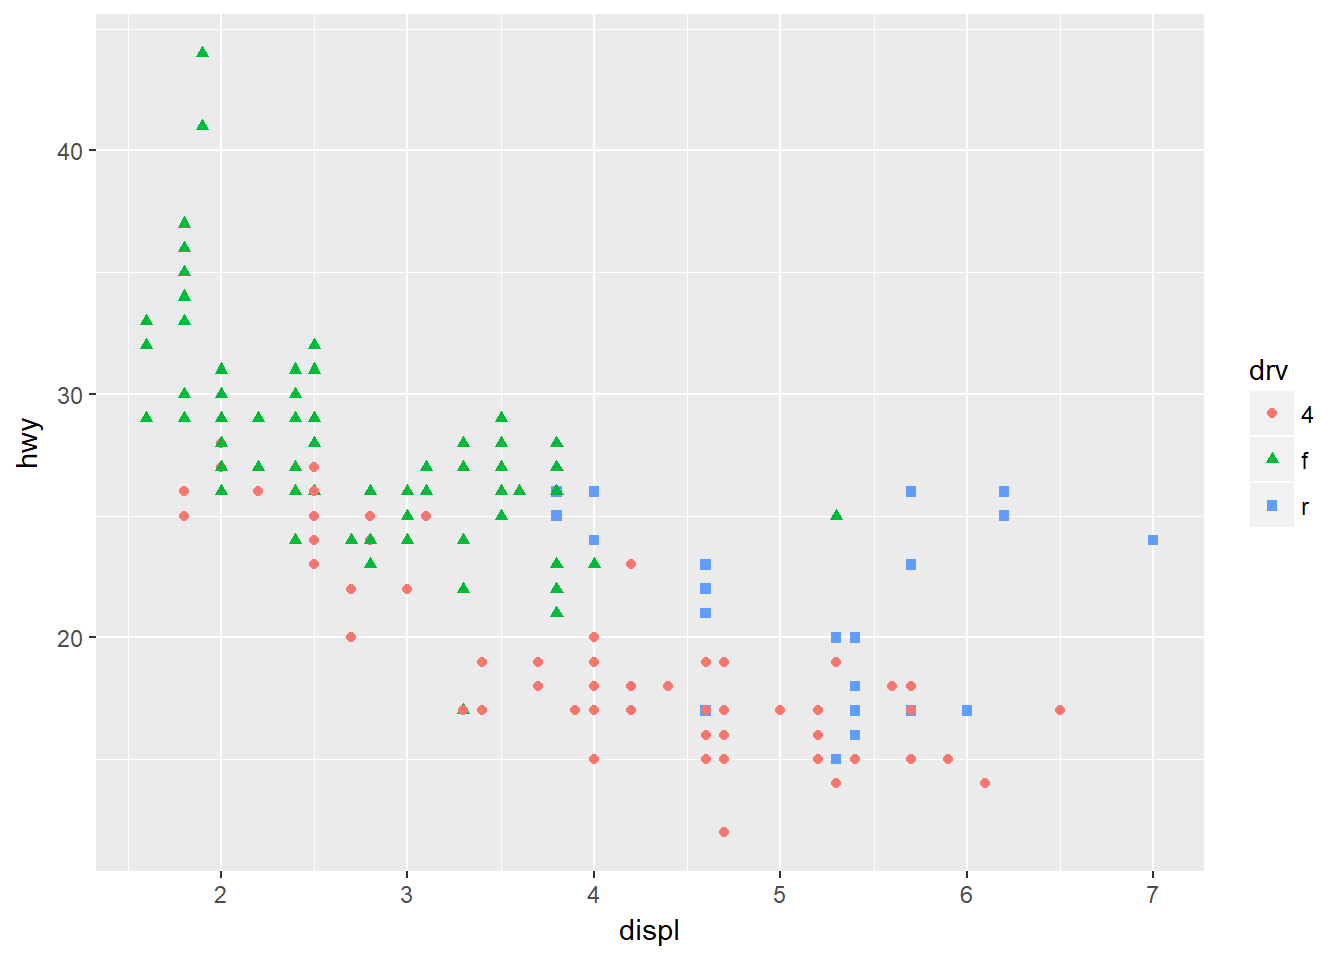
\includegraphics{R4DS_bookdown_files/figure-latex/unnamed-chunk-13-1.pdf}

Here, we map a continuous variable, \texttt{displ}, to \texttt{color}
and \texttt{size}.

\begin{Shaded}
\begin{Highlighting}[]
\KeywordTok{ggplot}\NormalTok{(}\DataTypeTok{data =}\NormalTok{ mpg) }\OperatorTok{+}
\StringTok{  }\KeywordTok{geom_point}\NormalTok{(}\DataTypeTok{mapping =} \KeywordTok{aes}\NormalTok{(}\DataTypeTok{x =}\NormalTok{ displ, }\DataTypeTok{y =}\NormalTok{ hwy, }\DataTypeTok{color =}\NormalTok{ displ, }\DataTypeTok{size =}\NormalTok{ displ))}
\end{Highlighting}
\end{Shaded}

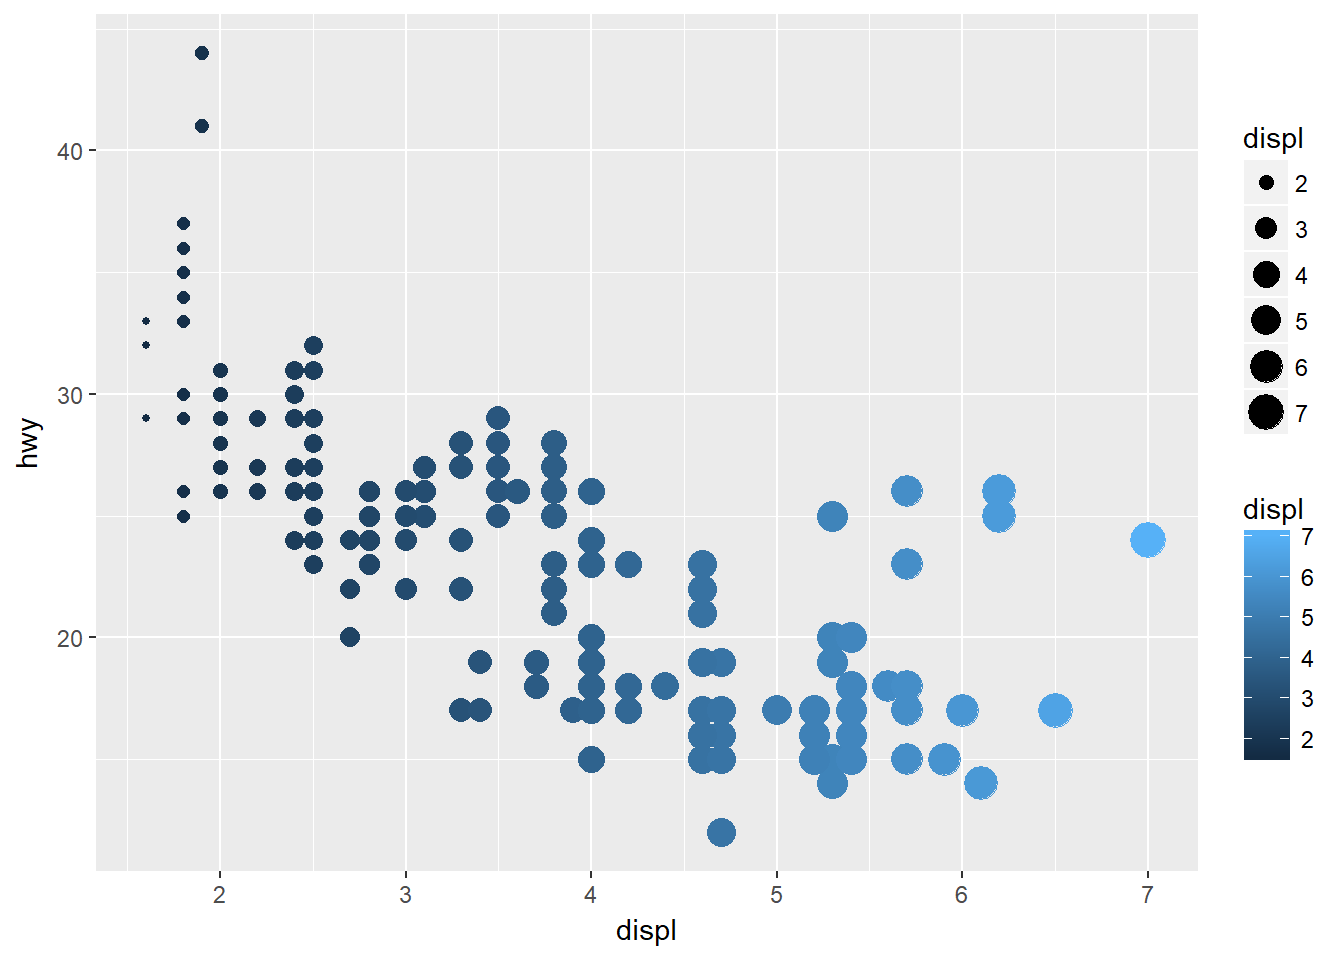
\includegraphics{R4DS_bookdown_files/figure-latex/unnamed-chunk-14-1.pdf}

\emph{5 - What does the \texttt{stroke} aesthetic do? What shapes does
it work with? (Hint: use \texttt{?geom\_point})}

\texttt{stroke} only works with shapes 21 - 24, which also comes with
the \texttt{fill} argument, which controls the color of the fill.
\texttt{size} argument controls the size of the fill part,
\texttt{stroke} controls the size of the stroke, and \texttt{color}
contools the color of the stroke. For example:

\begin{Shaded}
\begin{Highlighting}[]
\KeywordTok{ggplot}\NormalTok{(}\DataTypeTok{data =}\NormalTok{ mpg) }\OperatorTok{+}
\StringTok{  }\KeywordTok{geom_point}\NormalTok{(}\DataTypeTok{mapping =} \KeywordTok{aes}\NormalTok{(}\DataTypeTok{x =}\NormalTok{ displ, }\DataTypeTok{y =}\NormalTok{ hwy), }\DataTypeTok{shape =} \DecValTok{21}\NormalTok{,}
             \DataTypeTok{fill =} \StringTok{'red'}\NormalTok{, }\DataTypeTok{size =} \DecValTok{4}\NormalTok{, }\DataTypeTok{stroke =} \DecValTok{3}\NormalTok{, }\DataTypeTok{color =} \StringTok{'white'}\NormalTok{)}
\end{Highlighting}
\end{Shaded}

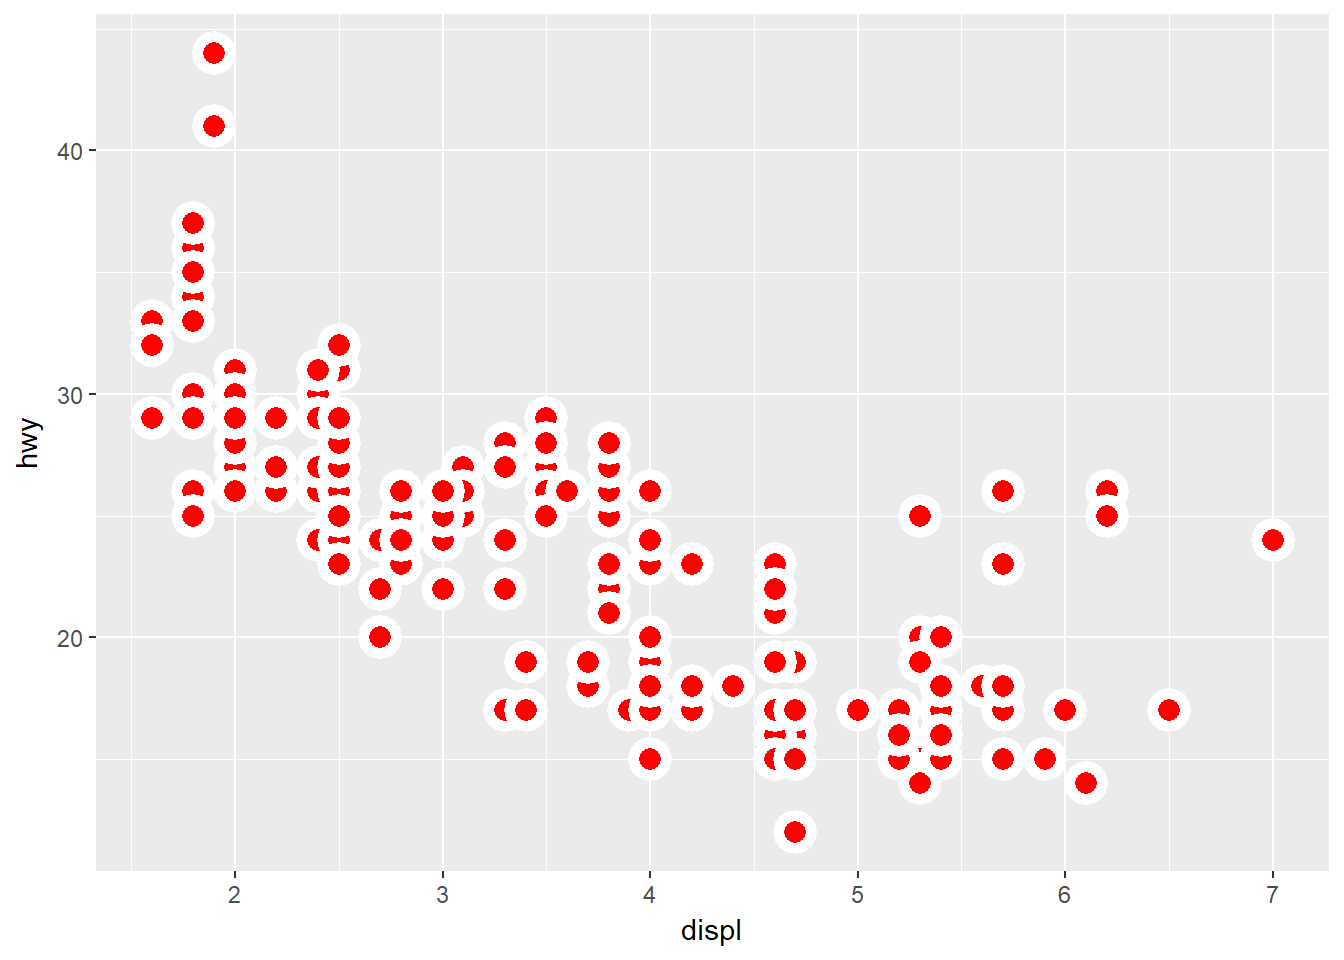
\includegraphics{R4DS_bookdown_files/figure-latex/unnamed-chunk-15-1.pdf}

\emph{6 - What happens if you map an aesthetic to something other than a
variable name, like \texttt{aes(colour\ =\ displ\ \textless{}\ 5)}?}

\begin{Shaded}
\begin{Highlighting}[]
\KeywordTok{ggplot}\NormalTok{(}\DataTypeTok{data =}\NormalTok{ mpg) }\OperatorTok{+}
\StringTok{  }\KeywordTok{geom_point}\NormalTok{(}\DataTypeTok{mapping =} \KeywordTok{aes}\NormalTok{(}\DataTypeTok{x =}\NormalTok{ displ, }\DataTypeTok{y =}\NormalTok{ hwy, }\DataTypeTok{color =}\NormalTok{ displ }\OperatorTok{<}\StringTok{ }\DecValTok{5}\NormalTok{))}
\end{Highlighting}
\end{Shaded}

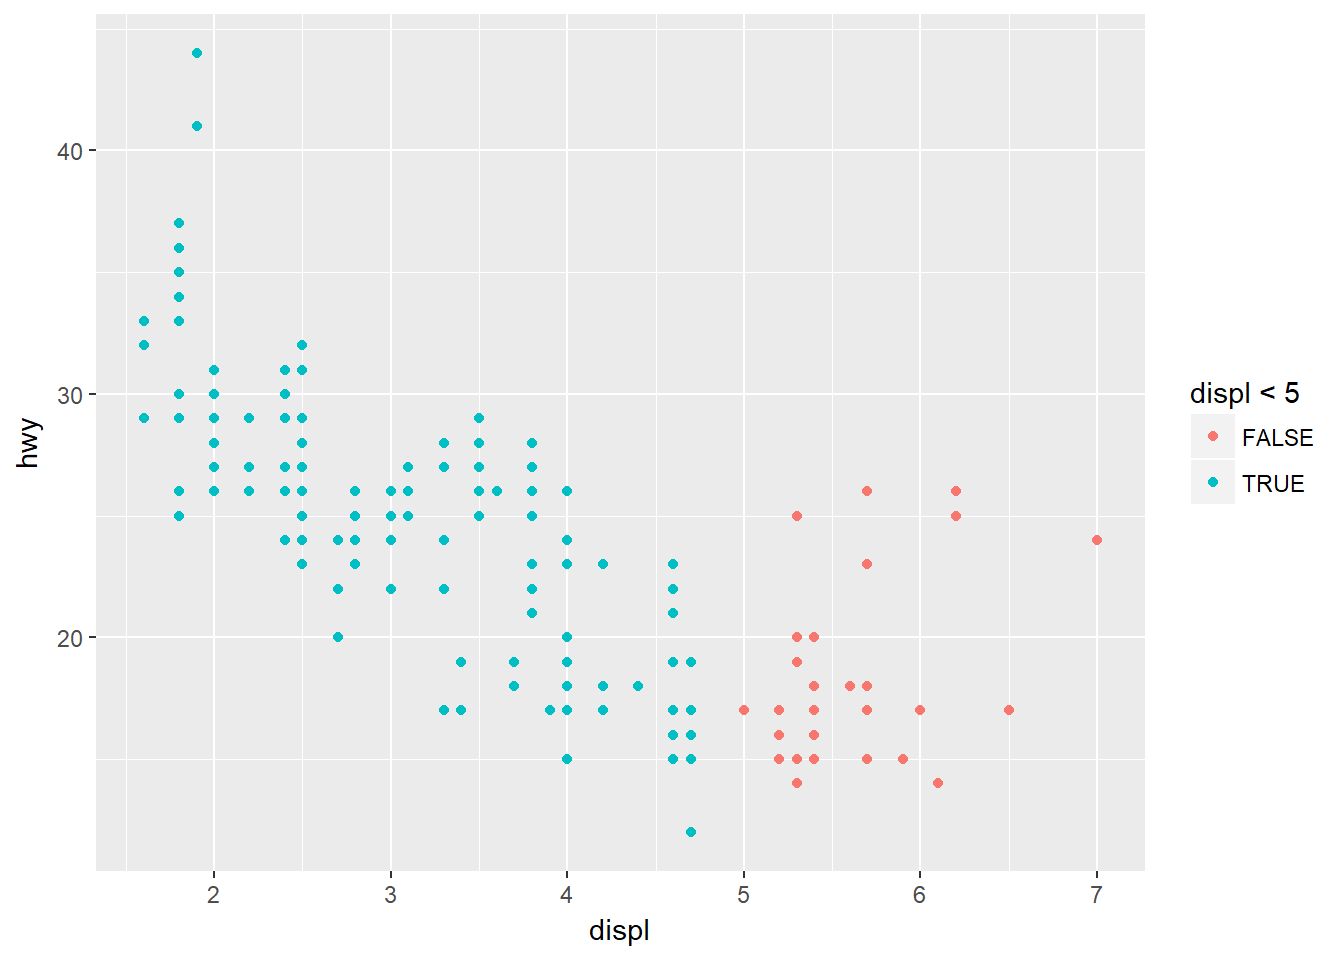
\includegraphics{R4DS_bookdown_files/figure-latex/unnamed-chunk-16-1.pdf}

As shown in the above scatter plots, ggplot evaluates
\texttt{displ\ \textless{}\ 5} and creates a temporary boolean variable
indicating whether the observations satisfy the specified condition, and
represents \texttt{TRUE} and \texttt{FALSE} with different colors.

\subsection{Common problems}\label{common-problems}

No exercises.

\subsection{Facets}\label{facets}

\subsubsection{Exercises}\label{exercises-2}

\emph{1 - What happens if you facet on a continuous variable?}

\begin{Shaded}
\begin{Highlighting}[]
\KeywordTok{ggplot}\NormalTok{(}\DataTypeTok{data =}\NormalTok{ mpg) }\OperatorTok{+}\StringTok{ }
\StringTok{  }\KeywordTok{geom_point}\NormalTok{(}\DataTypeTok{mapping =} \KeywordTok{aes}\NormalTok{(}\DataTypeTok{x =}\NormalTok{ displ, }\DataTypeTok{y =}\NormalTok{ hwy)) }\OperatorTok{+}\StringTok{ }
\StringTok{  }\KeywordTok{facet_wrap}\NormalTok{(}\OperatorTok{~}\StringTok{ }\NormalTok{cty, }\DataTypeTok{nrow =} \DecValTok{2}\NormalTok{)}
\end{Highlighting}
\end{Shaded}

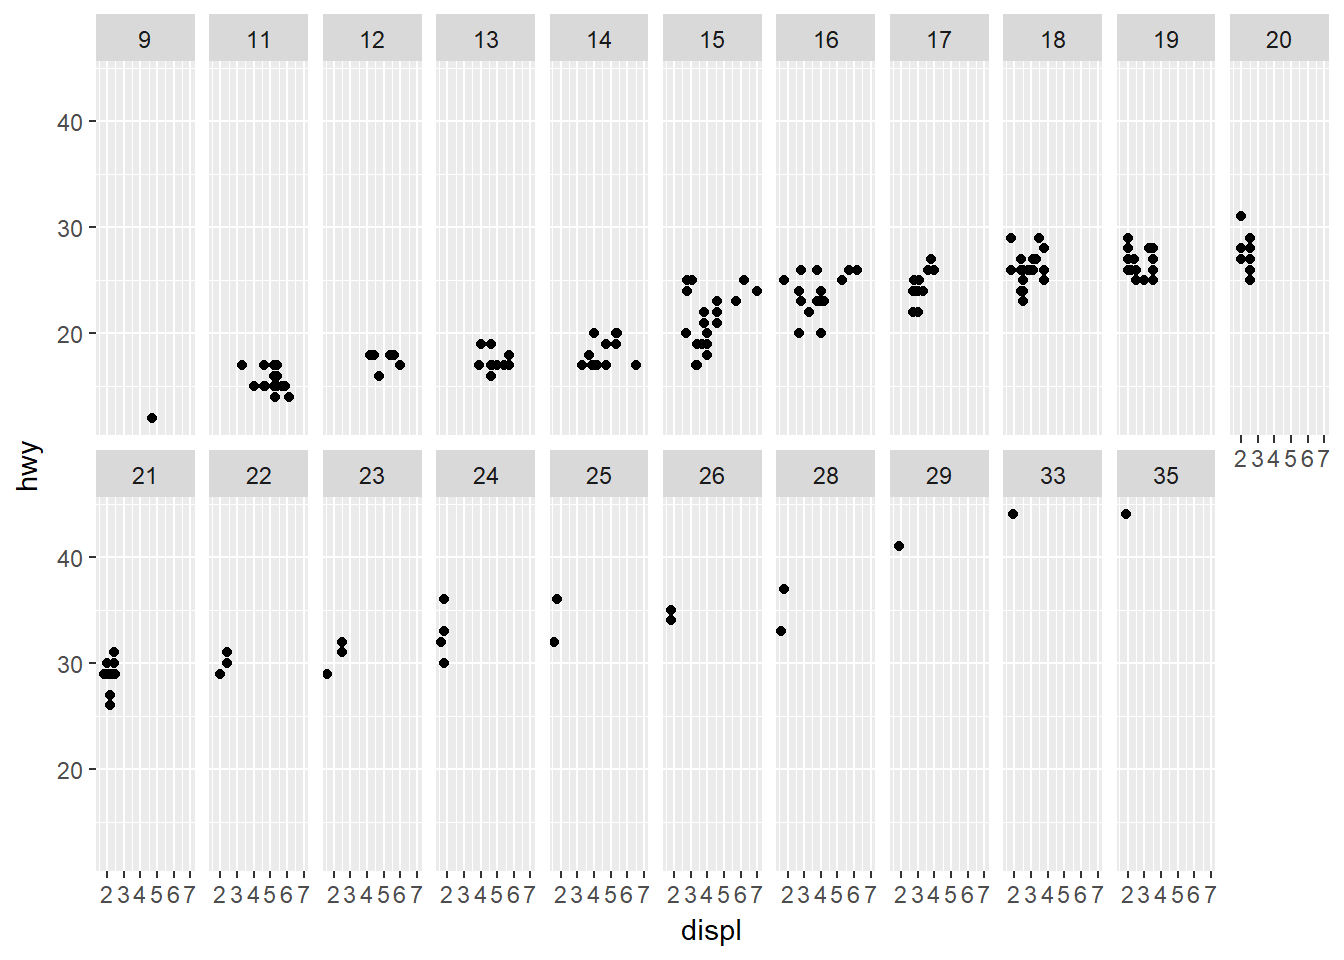
\includegraphics{R4DS_bookdown_files/figure-latex/unnamed-chunk-17-1.pdf}

Using \texttt{facet\_wrap()} with a continuous variable will work in
general, however, it might not be as useful as faceting on a categorical
variable with a few levels. The above plot shows \texttt{hwy} vs
\texttt{disp} scatter plots facetted by \texttt{cty}. What it does is
first converting the continuous variable to a factor, then displays
separate plots for each unique value.

\begin{Shaded}
\begin{Highlighting}[]
\KeywordTok{ggplot}\NormalTok{(}\DataTypeTok{data =}\NormalTok{ mpg) }\OperatorTok{+}\StringTok{ }
\StringTok{  }\KeywordTok{geom_point}\NormalTok{(}\DataTypeTok{mapping =} \KeywordTok{aes}\NormalTok{(}\DataTypeTok{x =}\NormalTok{ displ, }\DataTypeTok{y =}\NormalTok{ hwy)) }\OperatorTok{+}\StringTok{ }
\StringTok{  }\KeywordTok{facet_grid}\NormalTok{(cty }\OperatorTok{~}\StringTok{ }\NormalTok{year)}
\end{Highlighting}
\end{Shaded}

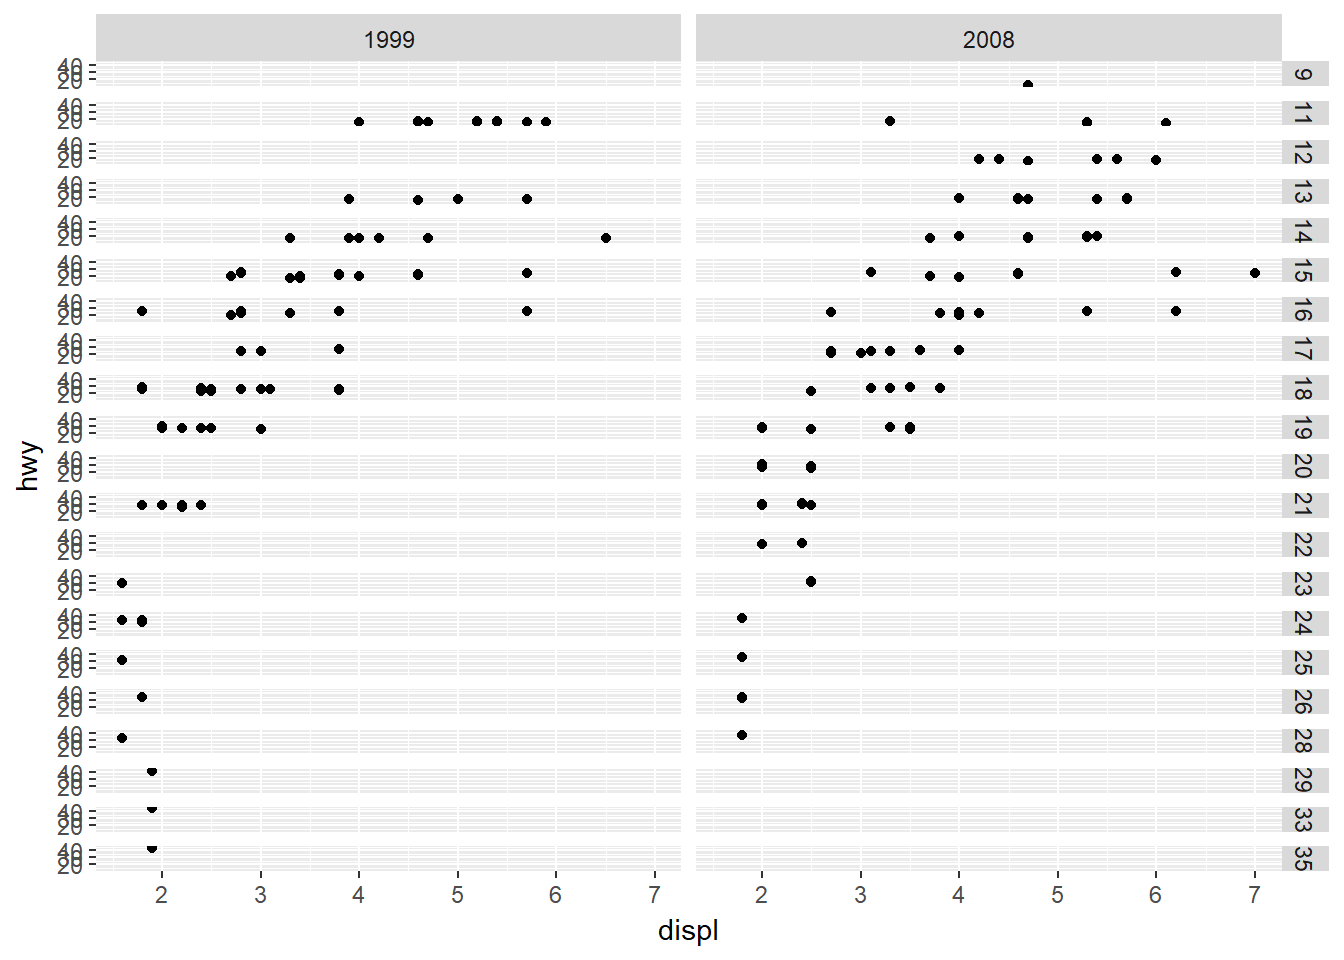
\includegraphics{R4DS_bookdown_files/figure-latex/unnamed-chunk-18-1.pdf}

Similarly, \texttt{facet\_grid()} works with continuous variables as
well.

\emph{2 - What do the empty cells in plot with
\texttt{facet\_grid(drv\ \textasciitilde{}\ cyl)} mean? How do they
relate to this plot?}

A plot with \texttt{facet\_grid(drv\ \textasciitilde{}\ cyl)}:

\begin{Shaded}
\begin{Highlighting}[]
\KeywordTok{ggplot}\NormalTok{(}\DataTypeTok{data =}\NormalTok{ mpg) }\OperatorTok{+}
\StringTok{  }\KeywordTok{geom_point}\NormalTok{(}\DataTypeTok{mapping =} \KeywordTok{aes}\NormalTok{(}\DataTypeTok{x =}\NormalTok{ displ, }\DataTypeTok{y=}\NormalTok{ hwy)) }\OperatorTok{+}\StringTok{ }
\StringTok{  }\KeywordTok{facet_grid}\NormalTok{(drv }\OperatorTok{~}\StringTok{ }\NormalTok{cyl)}
\end{Highlighting}
\end{Shaded}

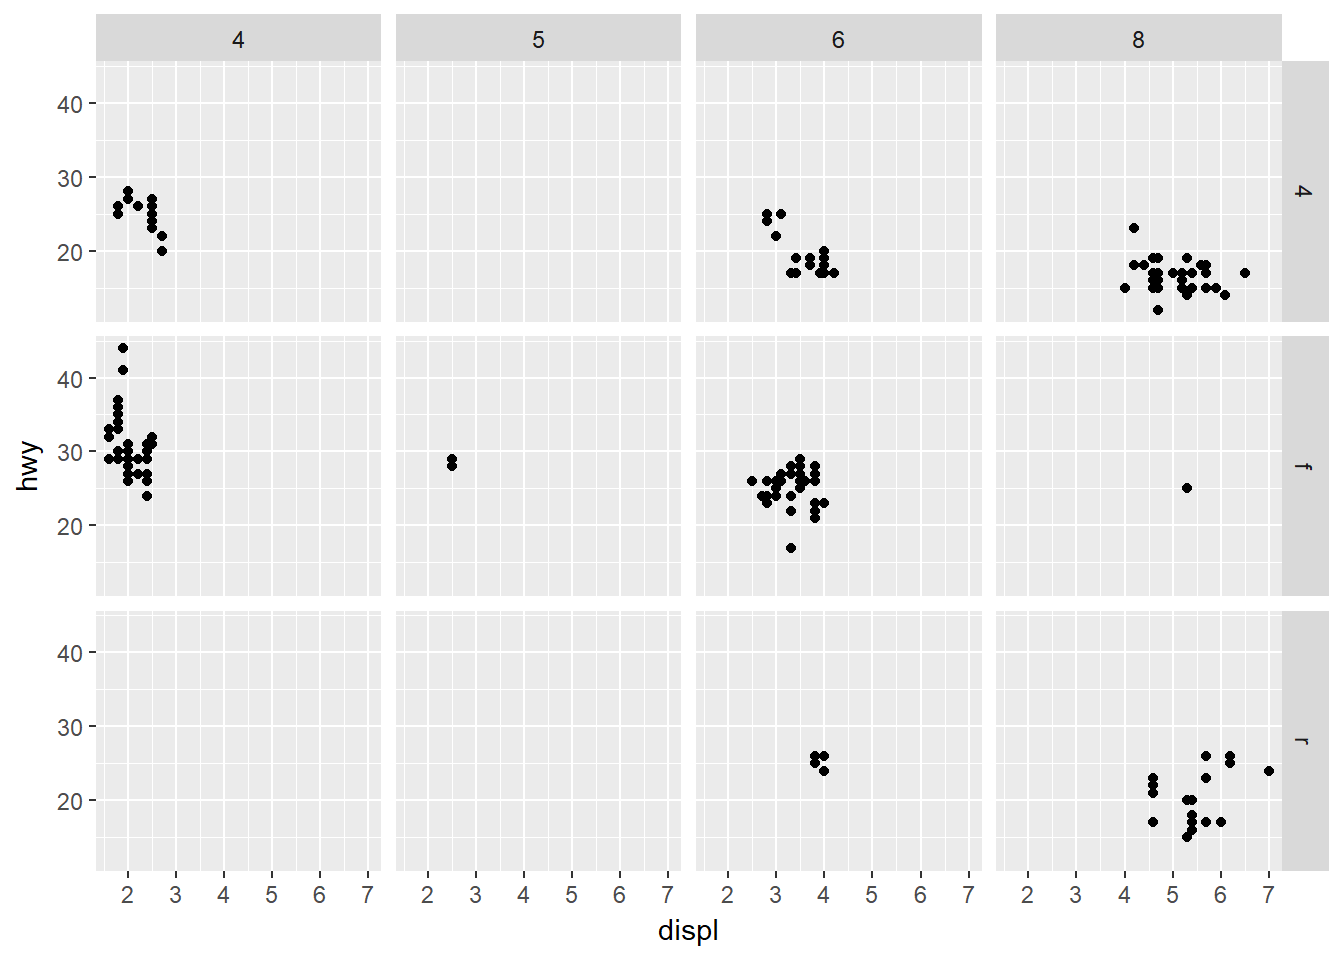
\includegraphics{R4DS_bookdown_files/figure-latex/unnamed-chunk-19-1.pdf}

Compared with the plot below:

\begin{Shaded}
\begin{Highlighting}[]
\KeywordTok{ggplot}\NormalTok{(}\DataTypeTok{data =}\NormalTok{ mpg) }\OperatorTok{+}\StringTok{ }
\StringTok{  }\KeywordTok{geom_point}\NormalTok{(}\DataTypeTok{mapping =} \KeywordTok{aes}\NormalTok{(}\DataTypeTok{x =}\NormalTok{ drv, }\DataTypeTok{y =}\NormalTok{ cyl))}
\end{Highlighting}
\end{Shaded}

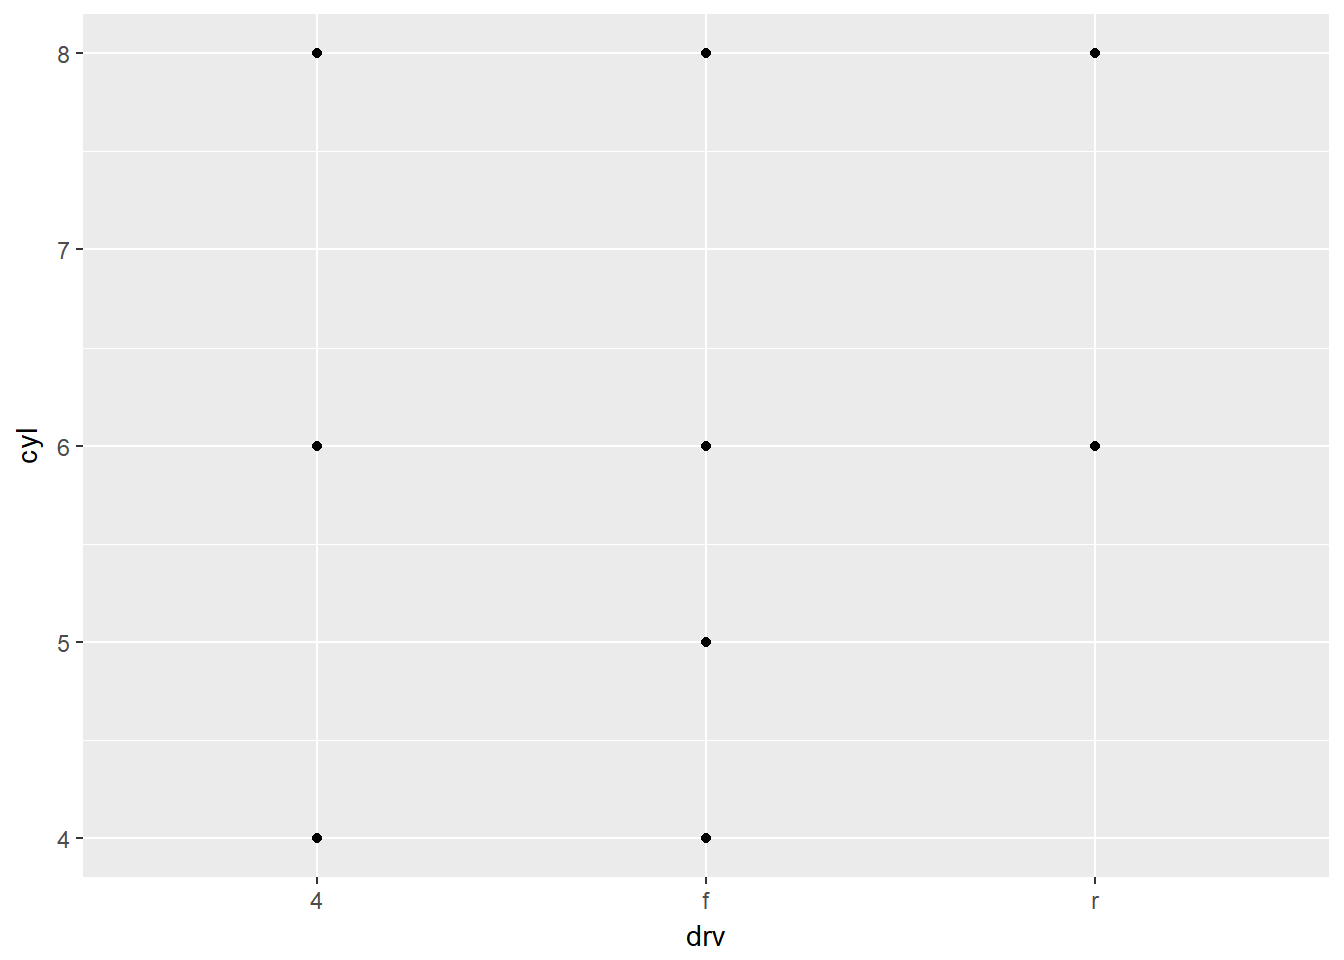
\includegraphics{R4DS_bookdown_files/figure-latex/unnamed-chunk-20-1.pdf}

The empty grids in \texttt{facet\_grid(drv\ \textasciitilde{}\ cyl)}
tell us that there are no observations in those particular combinations
of \texttt{cyl} and \texttt{drv}. The above scatter plot of \texttt{cyl}
vs \texttt{drv} gives us the same information.

\emph{3 - What plots does the following code make? What does . do?}

In \texttt{facet\_grid()}, rows are facetted by the variable on the left
hand side of \texttt{\textasciitilde{}}, and columns are facetted by the
variable on the right hand side of \texttt{\textasciitilde{}}. A
\texttt{.} simply means that there will be no facetting in the
dimension.

\begin{Shaded}
\begin{Highlighting}[]
\KeywordTok{ggplot}\NormalTok{(}\DataTypeTok{data =}\NormalTok{ mpg) }\OperatorTok{+}\StringTok{ }
\StringTok{  }\KeywordTok{geom_point}\NormalTok{(}\DataTypeTok{mapping =} \KeywordTok{aes}\NormalTok{(}\DataTypeTok{x =}\NormalTok{ displ, }\DataTypeTok{y =}\NormalTok{ hwy)) }\OperatorTok{+}
\StringTok{  }\KeywordTok{facet_grid}\NormalTok{(drv }\OperatorTok{~}\StringTok{ }\NormalTok{.)}
\end{Highlighting}
\end{Shaded}

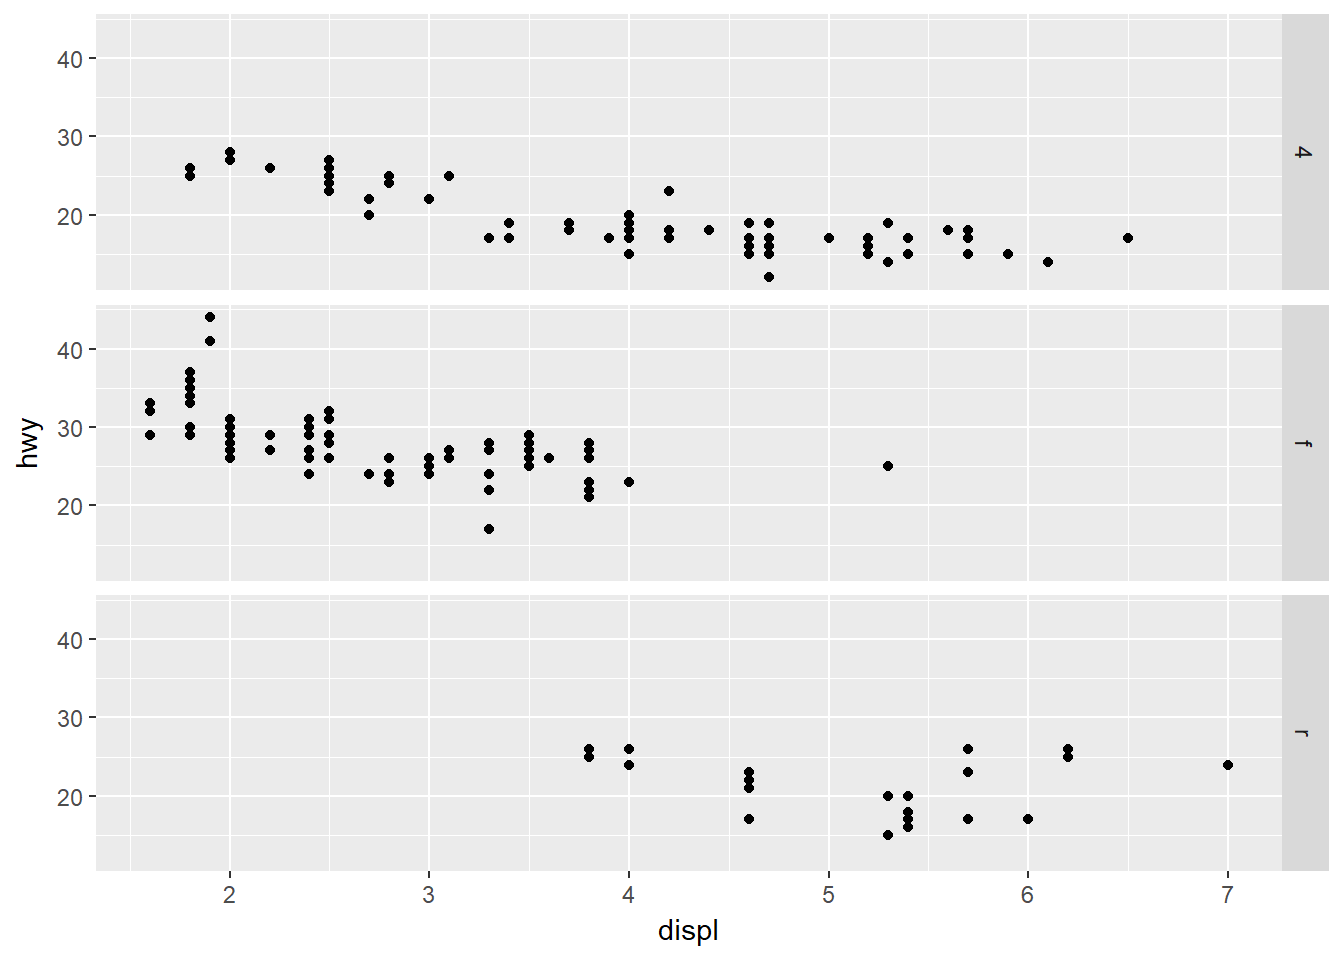
\includegraphics{R4DS_bookdown_files/figure-latex/unnamed-chunk-21-1.pdf}

\texttt{facet\_grid(drv\ \textasciitilde{}\ .\ )} - rows are facetted by
\texttt{drv}, and no facetting by columns

\begin{Shaded}
\begin{Highlighting}[]
\KeywordTok{ggplot}\NormalTok{(}\DataTypeTok{data =}\NormalTok{ mpg) }\OperatorTok{+}\StringTok{ }
\StringTok{  }\KeywordTok{geom_point}\NormalTok{(}\DataTypeTok{mapping =} \KeywordTok{aes}\NormalTok{(}\DataTypeTok{x =}\NormalTok{ displ, }\DataTypeTok{y =}\NormalTok{ hwy)) }\OperatorTok{+}
\StringTok{  }\KeywordTok{facet_grid}\NormalTok{(. }\OperatorTok{~}\StringTok{ }\NormalTok{cyl)}
\end{Highlighting}
\end{Shaded}

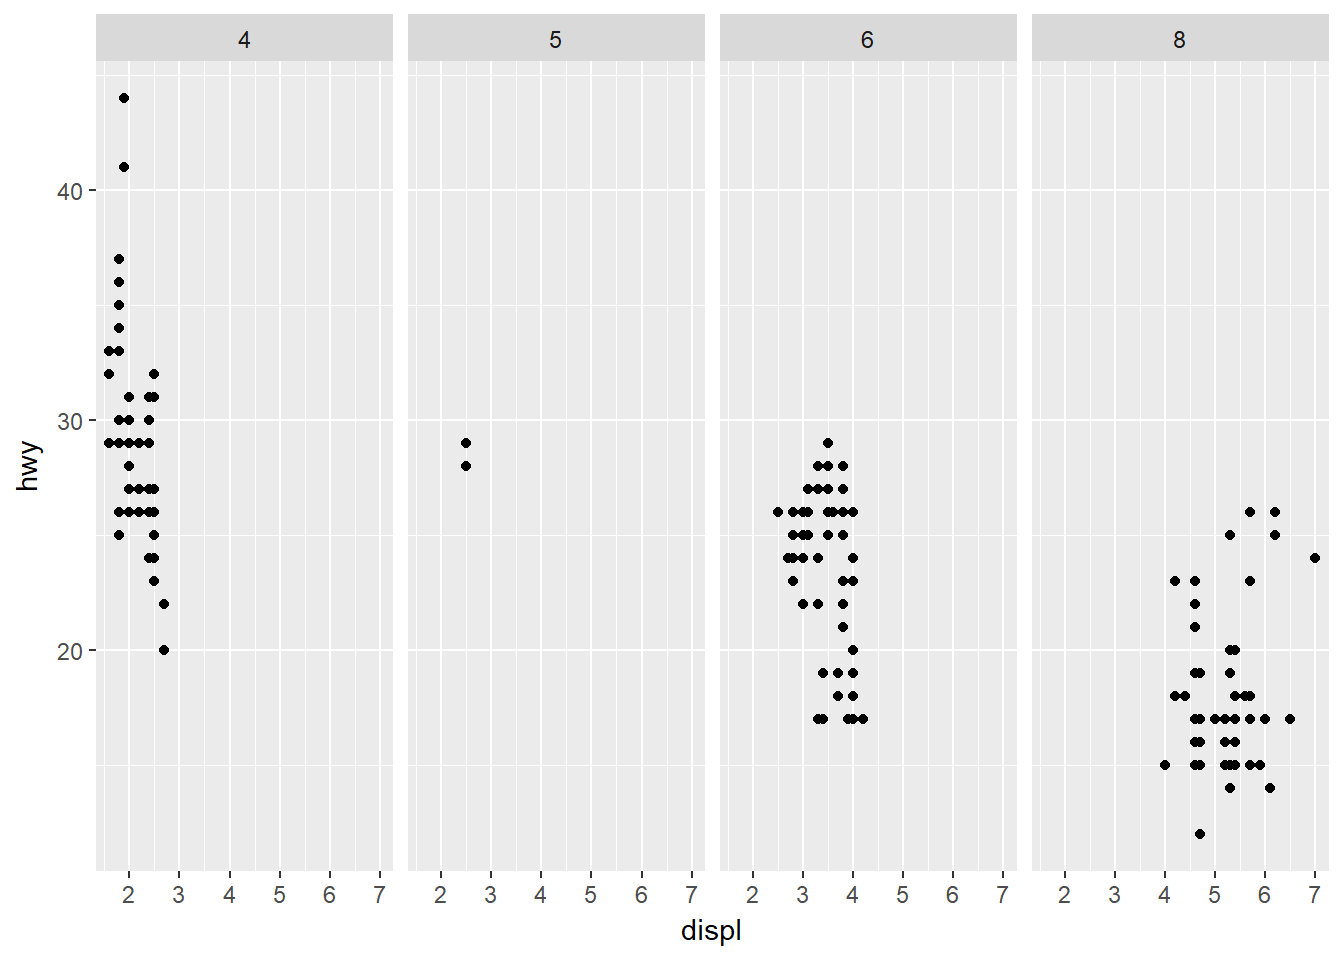
\includegraphics{R4DS_bookdown_files/figure-latex/unnamed-chunk-22-1.pdf}

\texttt{facet\_grid(.\ \textasciitilde{}\ cyl)} - columns are facetted
by \texttt{cyl}, and no facetting by rows.

\emph{4 - Take the first faceted plot in this section:}

\begin{Shaded}
\begin{Highlighting}[]
\KeywordTok{ggplot}\NormalTok{(}\DataTypeTok{data =}\NormalTok{ mpg) }\OperatorTok{+}\StringTok{ }
\StringTok{  }\KeywordTok{geom_point}\NormalTok{(}\DataTypeTok{mapping =} \KeywordTok{aes}\NormalTok{(}\DataTypeTok{x =}\NormalTok{ displ, }\DataTypeTok{y =}\NormalTok{ hwy)) }\OperatorTok{+}\StringTok{ }
\StringTok{  }\KeywordTok{facet_wrap}\NormalTok{(}\OperatorTok{~}\StringTok{ }\NormalTok{class, }\DataTypeTok{nrow =} \DecValTok{2}\NormalTok{)}
\end{Highlighting}
\end{Shaded}

\emph{What are the advantages to using faceting instead of the colour
aesthetic? What are the disadvantages? How might the balance change if
you had a larger dataset?}

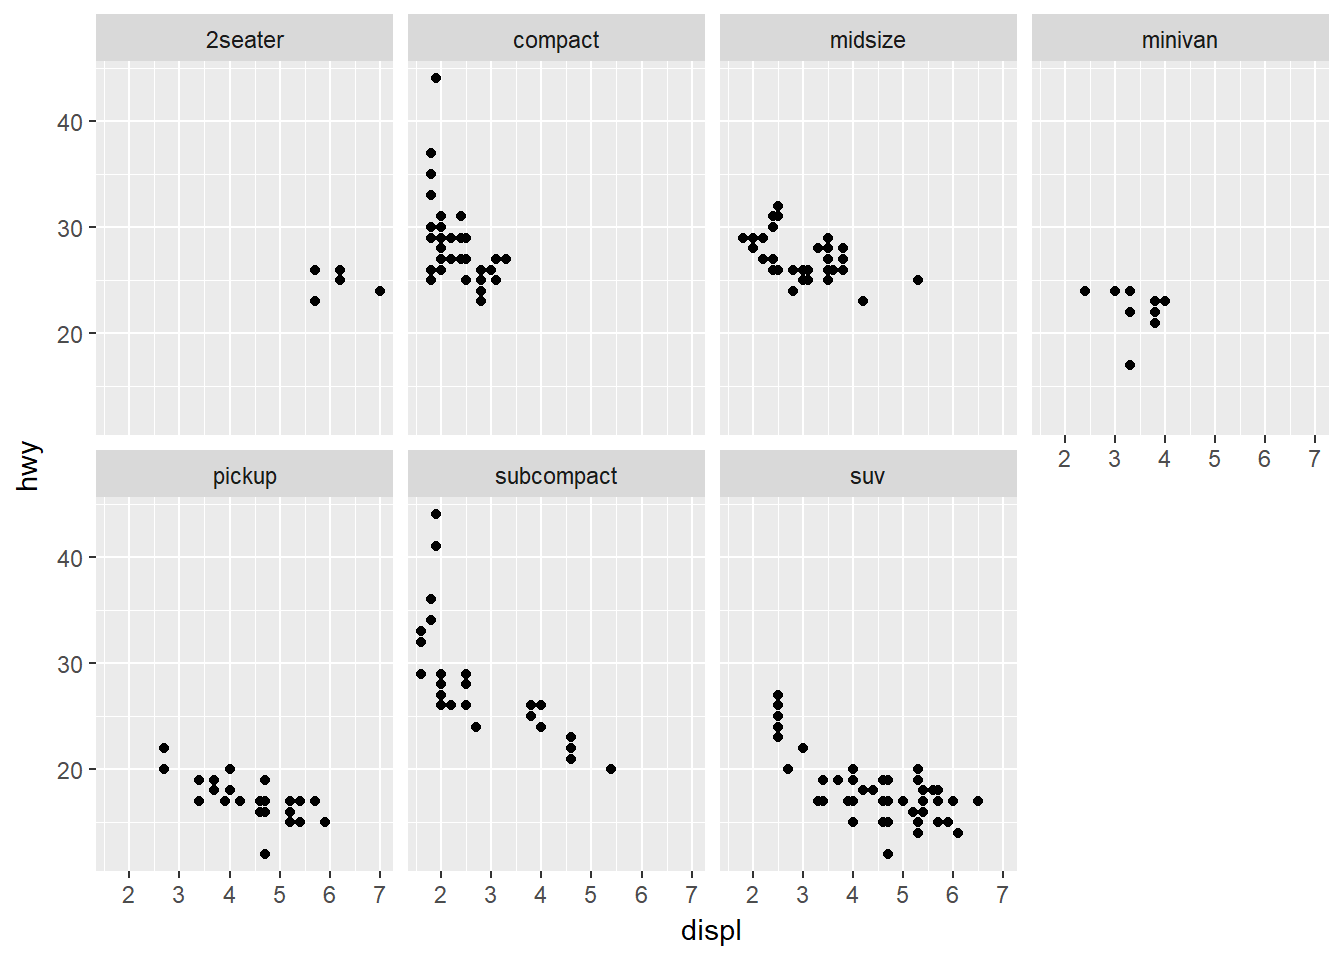
\includegraphics{R4DS_bookdown_files/figure-latex/unnamed-chunk-24-1.pdf}

One of the advantages of using facetting instead of coloring is to avoid
the possible confusion caused by having several distinct colors shown on
the same plot. As the number of unique levels in the mapping categorical
increases, it can be difficulty to distinguish between the differnet
colors.

A possible disadvantage in using facetting is that since the points are
on separate plots, direct comparisons might not be as straightforward.

\emph{5 - Read \texttt{?facet\_wrap}. What does \texttt{nrow} do? What
does \texttt{ncol} do? What other options control the layout of the
individual panels? Why doesn't \texttt{facet\_grid()} have \texttt{nrow}
and \texttt{ncol} argument?}

In \texttt{facet\_wrap()}, \texttt{nrow} and \texttt{ncol} defines the
number of rows and columns of the panels. \texttt{facet\_grid()} does
not have \texttt{nrow} and \texttt{ncol} since the number of rows and
columns are equal to the number of unique levels in the row/column
variables.

\emph{6 - When using facet\_grid() you should usually put the variable
with more unique levels in the columns. Why?}

One logical reason is that since the dependent variables are usually
plotted on the y-axis, it is much easier to compare the highs and lows
and the trends of the variables if the plots are placed side by side.

\subsection{Geometric objects}\label{geometric-objects}

\subsubsection{Exercises}\label{exercises-3}

\emph{1 - What geom would you use to draw a line chart? A boxplot? A
histogram? An area chart?}

\texttt{geom\_line()}, \texttt{geom\_boxplot()},
\texttt{geom\_histogram()}, and \texttt{geom\_area()}.

\emph{2 - Run this code in your head and predict what the output will
look like. Then, run the code in R and check your predictions.}

\begin{Shaded}
\begin{Highlighting}[]
\KeywordTok{ggplot}\NormalTok{(}\DataTypeTok{data =}\NormalTok{ mpg, }\DataTypeTok{mapping =} \KeywordTok{aes}\NormalTok{(}\DataTypeTok{x =}\NormalTok{ displ, }\DataTypeTok{y =}\NormalTok{ hwy, }\DataTypeTok{color =}\NormalTok{ drv)) }\OperatorTok{+}\StringTok{ }
\StringTok{  }\KeywordTok{geom_point}\NormalTok{() }\OperatorTok{+}\StringTok{ }
\StringTok{  }\KeywordTok{geom_smooth}\NormalTok{(}\DataTypeTok{se =} \OtherTok{FALSE}\NormalTok{)}
\end{Highlighting}
\end{Shaded}

\begin{verbatim}
## `geom_smooth()` using method = 'loess'
\end{verbatim}

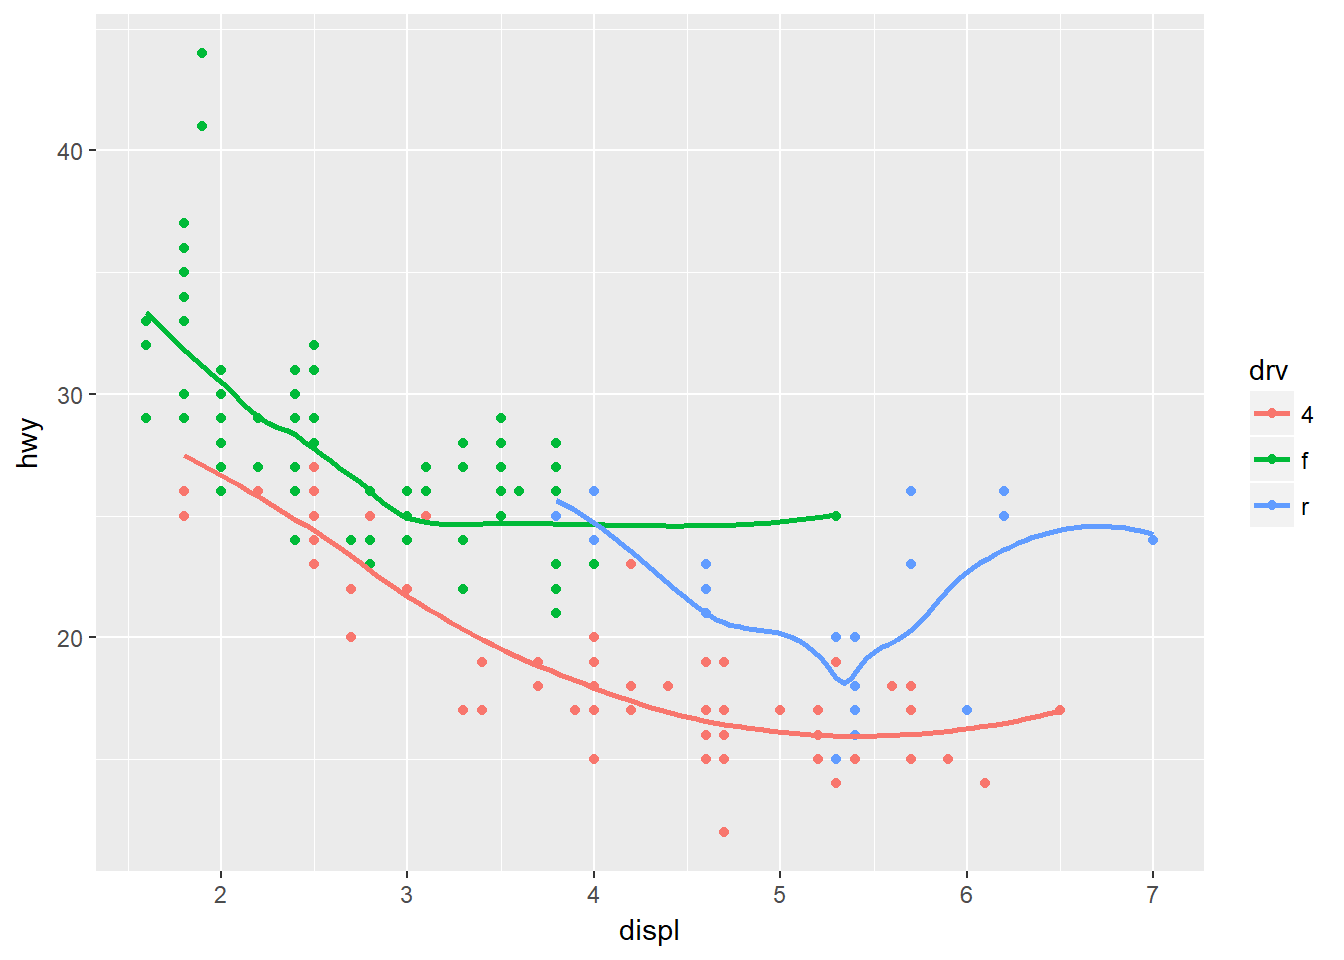
\includegraphics{R4DS_bookdown_files/figure-latex/unnamed-chunk-25-1.pdf}

Note: Since the mapping is defined in \texttt{ggplot()}, it is carried
over and applied to both \texttt{geom\_point()} and
\texttt{geom\_smooth()}.

\emph{3 - What does \texttt{show.legend\ =\ FALSE} do? What happens if
you remove it? Why do you think I used it earlier in the chapter?}

\texttt{show.legend\ =\ FALSE} hides the legned that is automatically
created when we map a variable to an aesthetic, like `color' or `size'.
Since the default is \texttt{TRUE}, removing this argument will always
result in the legend being displayed if there are variables mapped to
the asethetics. The last part of the question refers to this code:

\begin{Shaded}
\begin{Highlighting}[]
\KeywordTok{ggplot}\NormalTok{(}\DataTypeTok{data =}\NormalTok{ mpg) }\OperatorTok{+}
\StringTok{  }\KeywordTok{geom_smooth}\NormalTok{(}
    \DataTypeTok{mapping =} \KeywordTok{aes}\NormalTok{(}\DataTypeTok{x =}\NormalTok{ displ, }\DataTypeTok{y =}\NormalTok{ hwy, }\DataTypeTok{color =}\NormalTok{ drv),}
    \DataTypeTok{show.legend =} \OtherTok{FALSE}
\NormalTok{  )}
\end{Highlighting}
\end{Shaded}

\begin{verbatim}
## `geom_smooth()` using method = 'loess'
\end{verbatim}

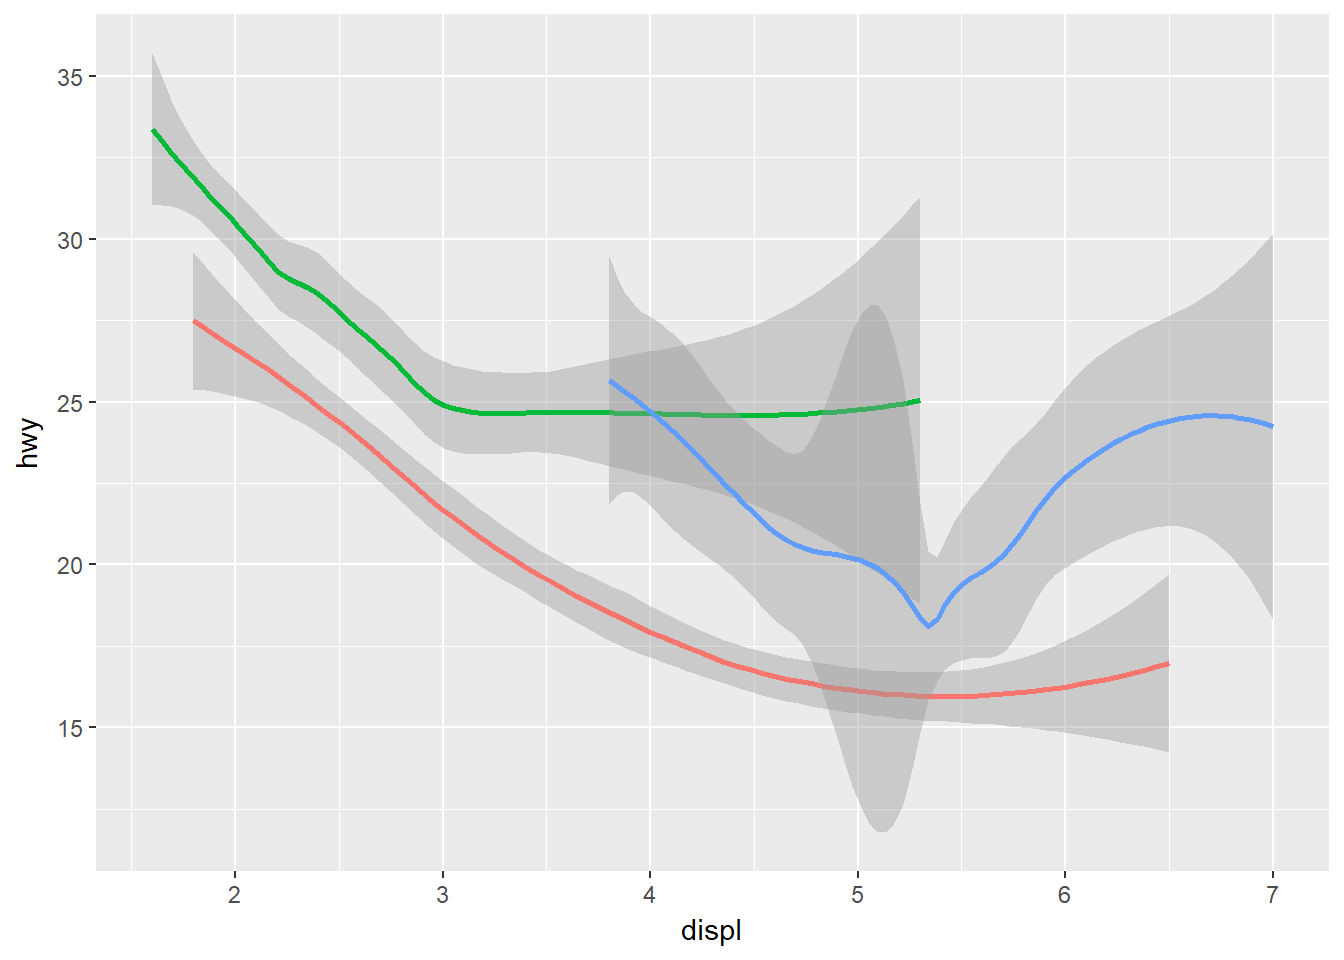
\includegraphics{R4DS_bookdown_files/figure-latex/unnamed-chunk-26-1.pdf}

Not exactly sure why, other than intentionally hiding the legend.

\emph{4 - What does the \texttt{se} argument to \texttt{geom\_smooth()}
do?}

The \texttt{se} argument controls whether the confidence interval around
the smooth curve is shown. The default value is \texttt{TRUE} and the
default level of CI is .95. The level of CI can be changed via the
\texttt{level} argument.

\emph{5 - Will these two graphs look different? Why/why not?}

\begin{Shaded}
\begin{Highlighting}[]
\KeywordTok{ggplot}\NormalTok{(}\DataTypeTok{data =}\NormalTok{ mpg, }\DataTypeTok{mapping =} \KeywordTok{aes}\NormalTok{(}\DataTypeTok{x =}\NormalTok{ displ, }\DataTypeTok{y =}\NormalTok{ hwy)) }\OperatorTok{+}\StringTok{ }
\StringTok{  }\KeywordTok{geom_point}\NormalTok{() }\OperatorTok{+}\StringTok{ }
\StringTok{  }\KeywordTok{geom_smooth}\NormalTok{()}

\KeywordTok{ggplot}\NormalTok{() }\OperatorTok{+}\StringTok{ }
\StringTok{  }\KeywordTok{geom_point}\NormalTok{(}\DataTypeTok{data =}\NormalTok{ mpg, }\DataTypeTok{mapping =} \KeywordTok{aes}\NormalTok{(}\DataTypeTok{x =}\NormalTok{ displ, }\DataTypeTok{y =}\NormalTok{ hwy)) }\OperatorTok{+}\StringTok{ }
\StringTok{  }\KeywordTok{geom_smooth}\NormalTok{(}\DataTypeTok{data =}\NormalTok{ mpg, }\DataTypeTok{mapping =} \KeywordTok{aes}\NormalTok{(}\DataTypeTok{x =}\NormalTok{ displ, }\DataTypeTok{y =}\NormalTok{ hwy))}
\end{Highlighting}
\end{Shaded}

The two graphs will look exactly the same. In the first code,
\texttt{data} and \texttt{mapping} are both defined in \texttt{ggplot()}
and are carried over to the geoms. In the second code, \texttt{data} and
\texttt{mapping} are defined individually in each geom.

\emph{6 - Recreate the R code necessary to generate the following
graphs.}

The codes to recreate the 6 plots are shown below. (Note - not sure
about the sizes so the \texttt{size} argument was skipped.)

\begin{Shaded}
\begin{Highlighting}[]
\KeywordTok{ggplot}\NormalTok{(}\DataTypeTok{data =}\NormalTok{ mpg, }\DataTypeTok{mapping =} \KeywordTok{aes}\NormalTok{(}\DataTypeTok{y =}\NormalTok{ hwy, }\DataTypeTok{x =}\NormalTok{ displ)) }\OperatorTok{+}\StringTok{ }
\StringTok{  }\KeywordTok{geom_point}\NormalTok{() }\OperatorTok{+}
\StringTok{  }\KeywordTok{geom_smooth}\NormalTok{(}\DataTypeTok{se =} \OtherTok{FALSE}\NormalTok{)}
\end{Highlighting}
\end{Shaded}

\begin{verbatim}
## `geom_smooth()` using method = 'loess'
\end{verbatim}

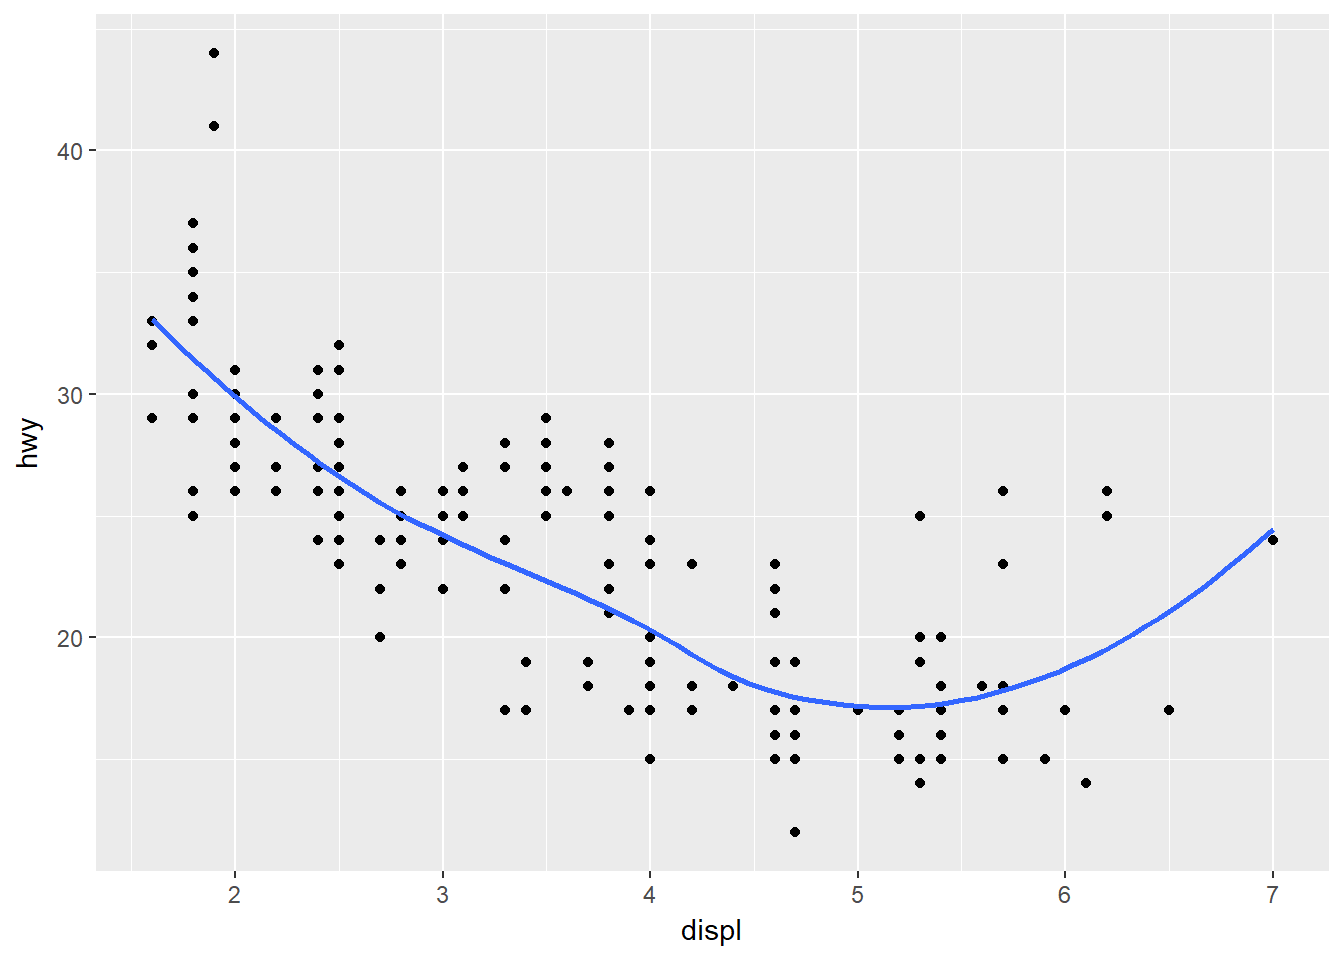
\includegraphics{R4DS_bookdown_files/figure-latex/unnamed-chunk-28-1.pdf}

\begin{Shaded}
\begin{Highlighting}[]
\KeywordTok{ggplot}\NormalTok{(}\DataTypeTok{data =}\NormalTok{ mpg, }\DataTypeTok{mapping =} \KeywordTok{aes}\NormalTok{(}\DataTypeTok{y =}\NormalTok{ hwy, }\DataTypeTok{x =}\NormalTok{ displ)) }\OperatorTok{+}\StringTok{ }
\StringTok{  }\KeywordTok{geom_point}\NormalTok{() }\OperatorTok{+}
\StringTok{  }\KeywordTok{geom_smooth}\NormalTok{(}\DataTypeTok{mapping =} \KeywordTok{aes}\NormalTok{(}\DataTypeTok{group =}\NormalTok{ drv), }\DataTypeTok{se =} \OtherTok{FALSE}\NormalTok{, }\DataTypeTok{show.legend =} \OtherTok{FALSE}\NormalTok{)}
\end{Highlighting}
\end{Shaded}

\begin{verbatim}
## `geom_smooth()` using method = 'loess'
\end{verbatim}

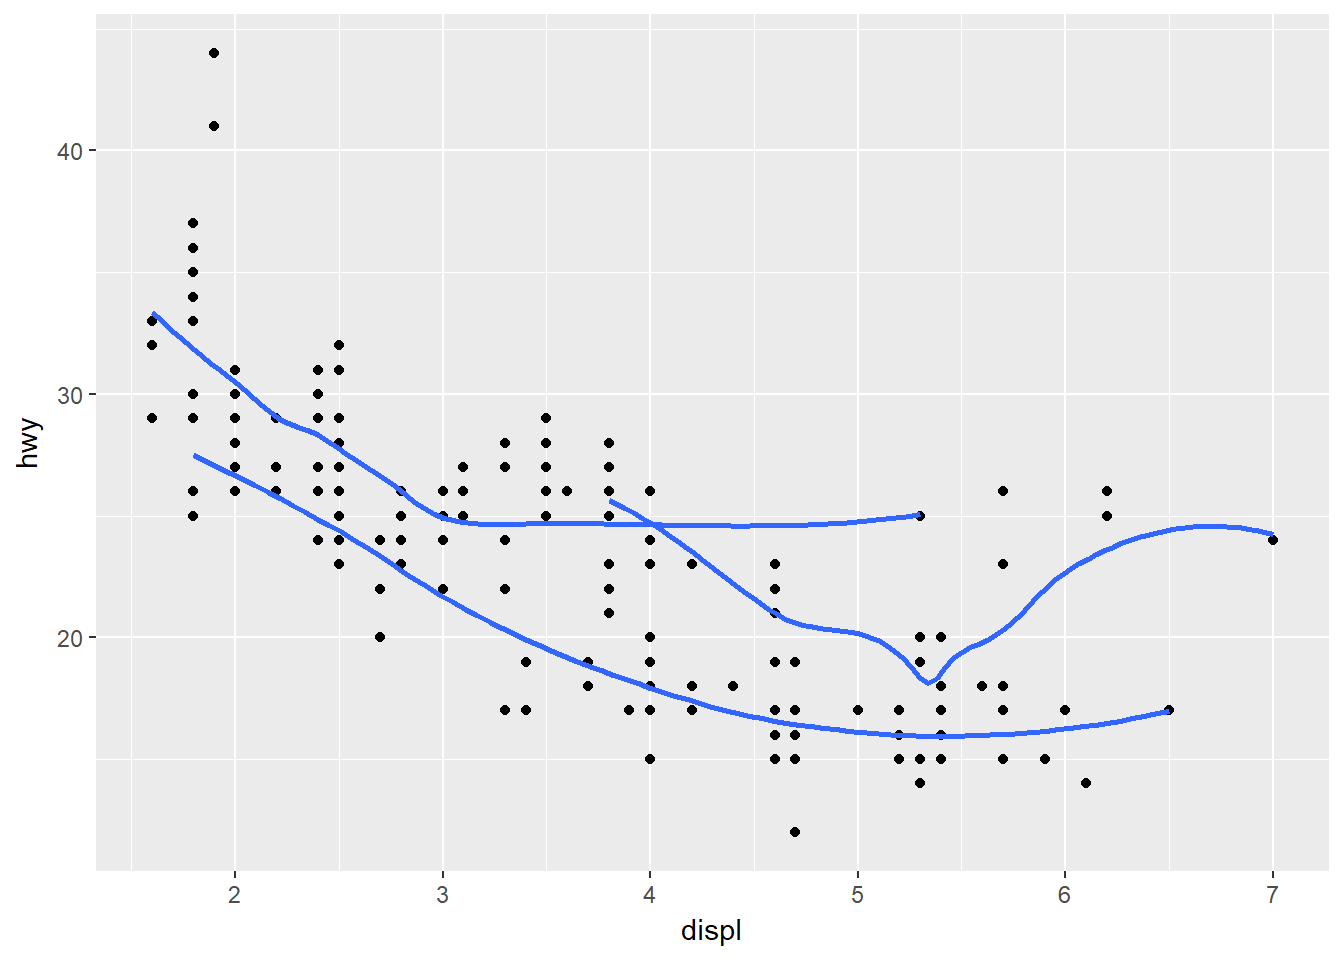
\includegraphics{R4DS_bookdown_files/figure-latex/unnamed-chunk-29-1.pdf}

\begin{Shaded}
\begin{Highlighting}[]
\KeywordTok{ggplot}\NormalTok{(}\DataTypeTok{data =}\NormalTok{ mpg, }\DataTypeTok{mapping =} \KeywordTok{aes}\NormalTok{(}\DataTypeTok{y =}\NormalTok{ hwy, }\DataTypeTok{x =}\NormalTok{ displ)) }\OperatorTok{+}\StringTok{ }
\StringTok{  }\KeywordTok{geom_point}\NormalTok{(}\DataTypeTok{mapping =} \KeywordTok{aes}\NormalTok{(}\DataTypeTok{color =}\NormalTok{ drv)) }\OperatorTok{+}
\StringTok{  }\KeywordTok{geom_smooth}\NormalTok{(}\DataTypeTok{mapping =} \KeywordTok{aes}\NormalTok{(}\DataTypeTok{color =}\NormalTok{ drv, }\DataTypeTok{group =}\NormalTok{ drv), }\DataTypeTok{se =} \OtherTok{FALSE}\NormalTok{)}
\end{Highlighting}
\end{Shaded}

\begin{verbatim}
## `geom_smooth()` using method = 'loess'
\end{verbatim}

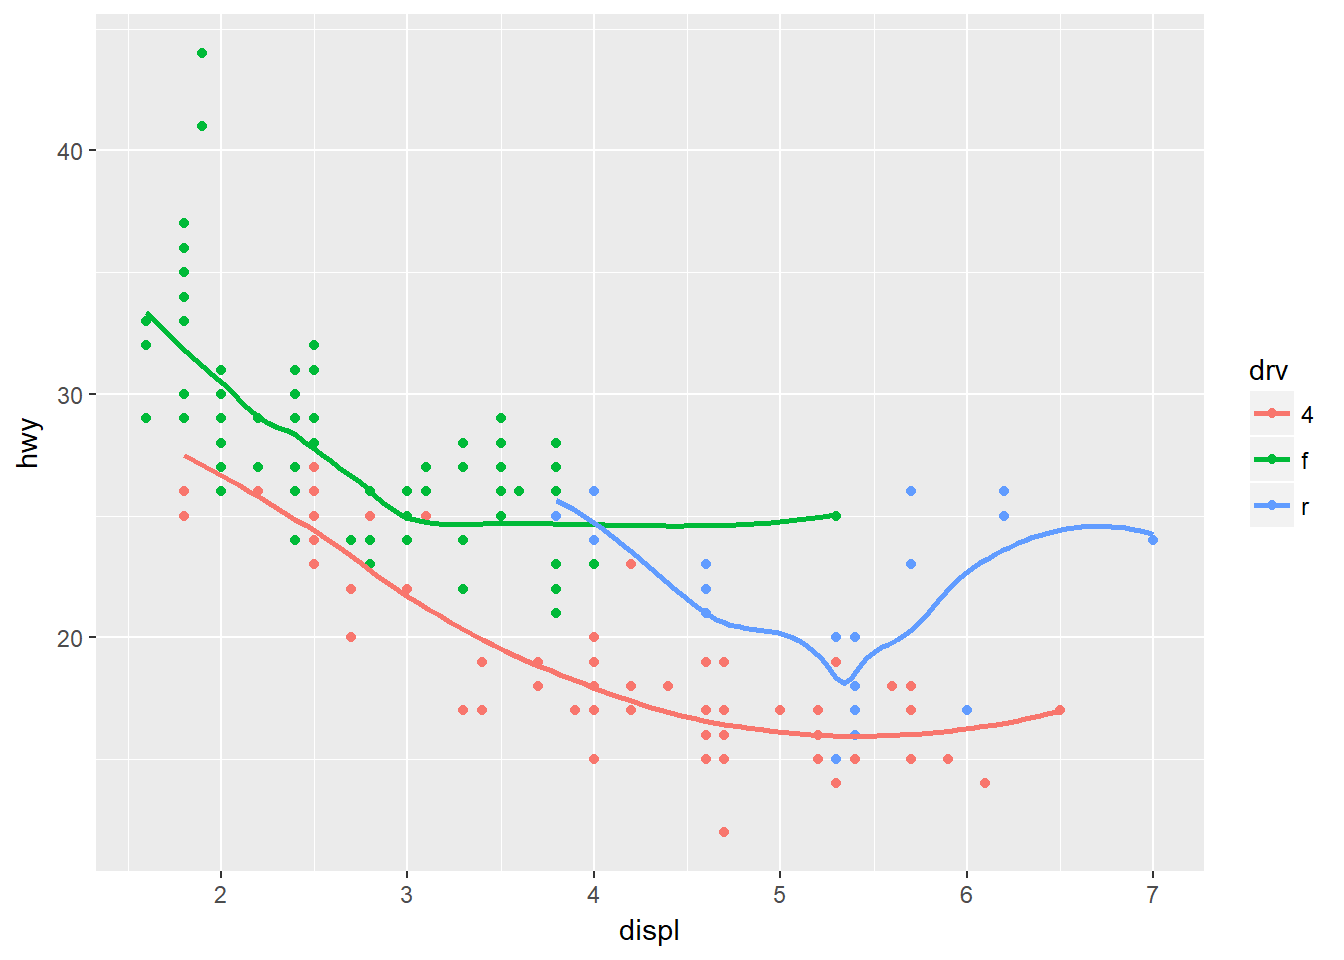
\includegraphics{R4DS_bookdown_files/figure-latex/unnamed-chunk-30-1.pdf}

\begin{Shaded}
\begin{Highlighting}[]
\KeywordTok{ggplot}\NormalTok{(}\DataTypeTok{data =}\NormalTok{ mpg, }\DataTypeTok{mapping =} \KeywordTok{aes}\NormalTok{(}\DataTypeTok{y =}\NormalTok{ hwy, }\DataTypeTok{x =}\NormalTok{ displ)) }\OperatorTok{+}\StringTok{ }
\StringTok{  }\KeywordTok{geom_point}\NormalTok{(}\DataTypeTok{mapping =} \KeywordTok{aes}\NormalTok{(}\DataTypeTok{color =}\NormalTok{ drv)) }\OperatorTok{+}
\StringTok{  }\KeywordTok{geom_smooth}\NormalTok{(}\DataTypeTok{se =} \OtherTok{FALSE}\NormalTok{)}
\end{Highlighting}
\end{Shaded}

\begin{verbatim}
## `geom_smooth()` using method = 'loess'
\end{verbatim}

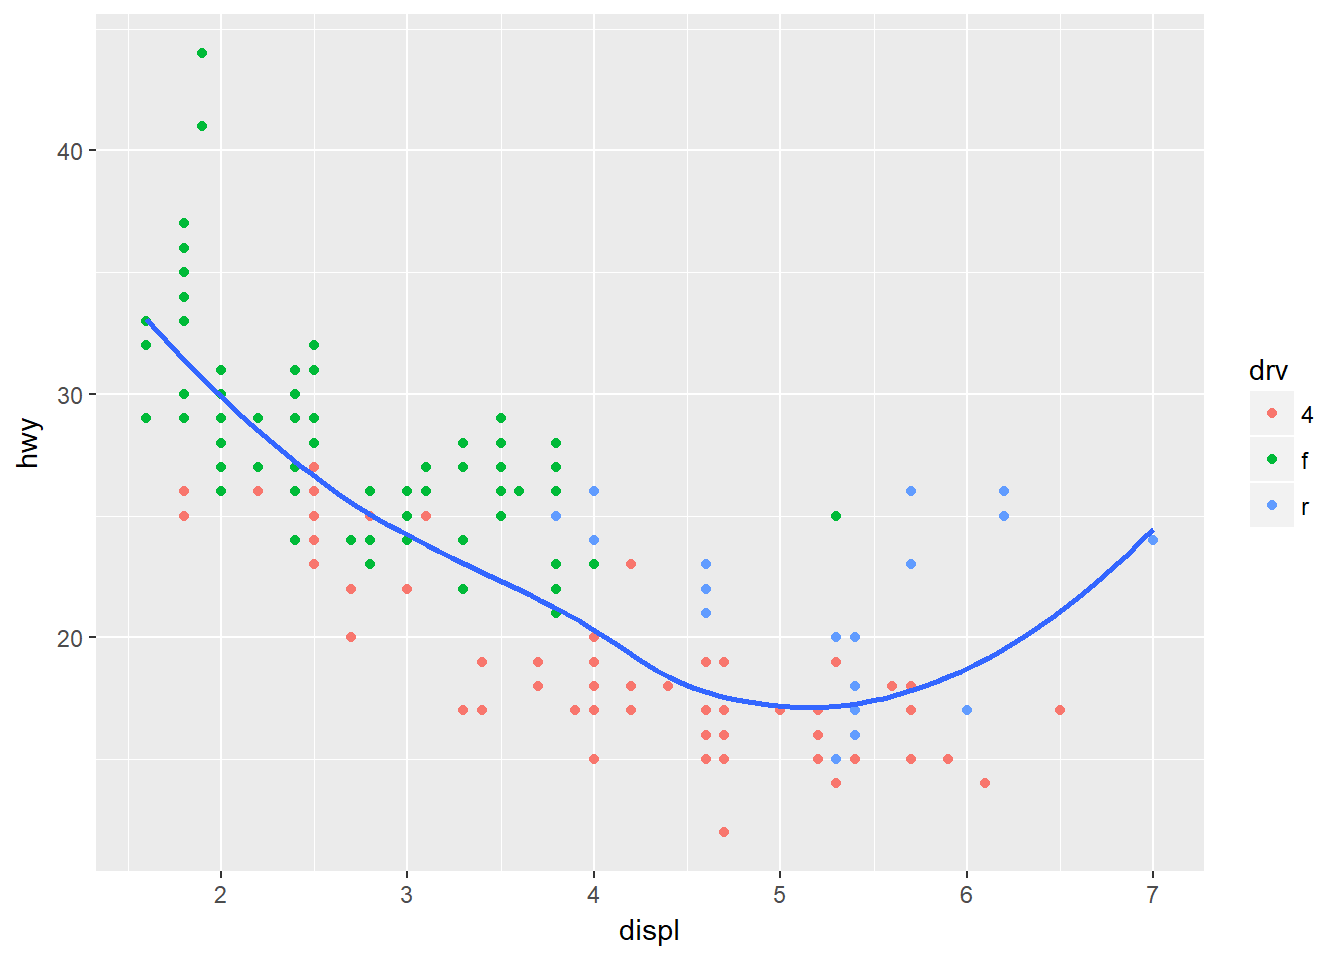
\includegraphics{R4DS_bookdown_files/figure-latex/unnamed-chunk-31-1.pdf}

\begin{Shaded}
\begin{Highlighting}[]
\KeywordTok{ggplot}\NormalTok{(}\DataTypeTok{data =}\NormalTok{ mpg, }\DataTypeTok{mapping =} \KeywordTok{aes}\NormalTok{(}\DataTypeTok{y =}\NormalTok{ hwy, }\DataTypeTok{x =}\NormalTok{ displ)) }\OperatorTok{+}\StringTok{ }
\StringTok{  }\KeywordTok{geom_point}\NormalTok{(}\DataTypeTok{mapping =} \KeywordTok{aes}\NormalTok{(}\DataTypeTok{color =}\NormalTok{ drv)) }\OperatorTok{+}
\StringTok{  }\KeywordTok{geom_smooth}\NormalTok{(}\DataTypeTok{mapping =} \KeywordTok{aes}\NormalTok{(}\DataTypeTok{linetype =}\NormalTok{ drv), }\DataTypeTok{se =} \OtherTok{FALSE}\NormalTok{)}
\end{Highlighting}
\end{Shaded}

\begin{verbatim}
## `geom_smooth()` using method = 'loess'
\end{verbatim}

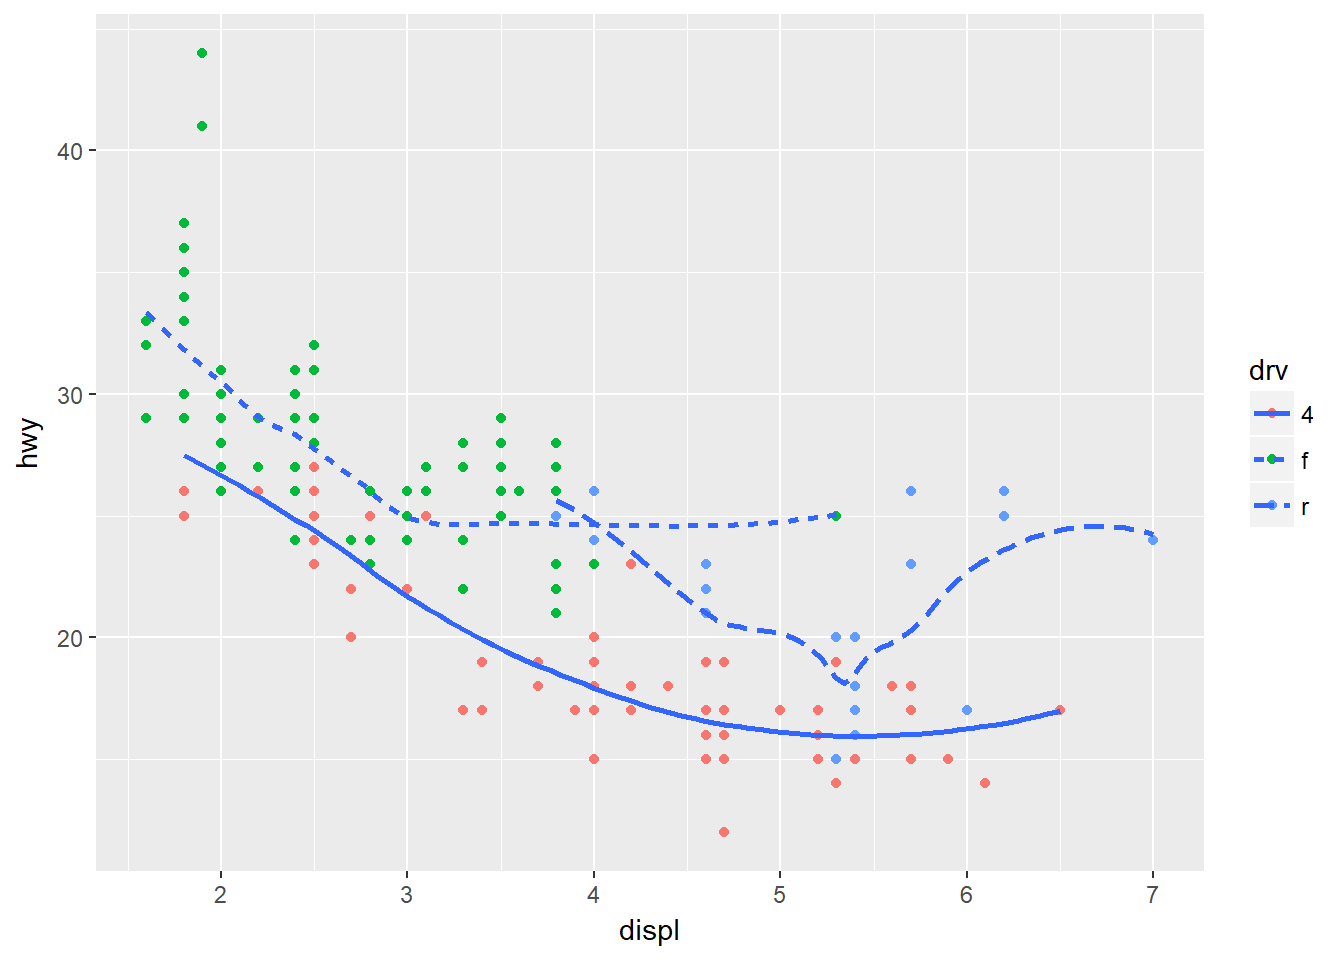
\includegraphics{R4DS_bookdown_files/figure-latex/unnamed-chunk-32-1.pdf}

\begin{Shaded}
\begin{Highlighting}[]
\KeywordTok{ggplot}\NormalTok{(}\DataTypeTok{data =}\NormalTok{ mpg, }\DataTypeTok{mapping =} \KeywordTok{aes}\NormalTok{(}\DataTypeTok{y =}\NormalTok{ hwy, }\DataTypeTok{x =}\NormalTok{ displ)) }\OperatorTok{+}\StringTok{ }
\StringTok{  }\KeywordTok{geom_point}\NormalTok{(}\DataTypeTok{mapping =} \KeywordTok{aes}\NormalTok{(}\DataTypeTok{fill =}\NormalTok{ drv), }\DataTypeTok{color =} \StringTok{'white'}\NormalTok{, }\DataTypeTok{stroke =} \DecValTok{2}\NormalTok{, }\DataTypeTok{shape =} \DecValTok{21}\NormalTok{)}
\end{Highlighting}
\end{Shaded}

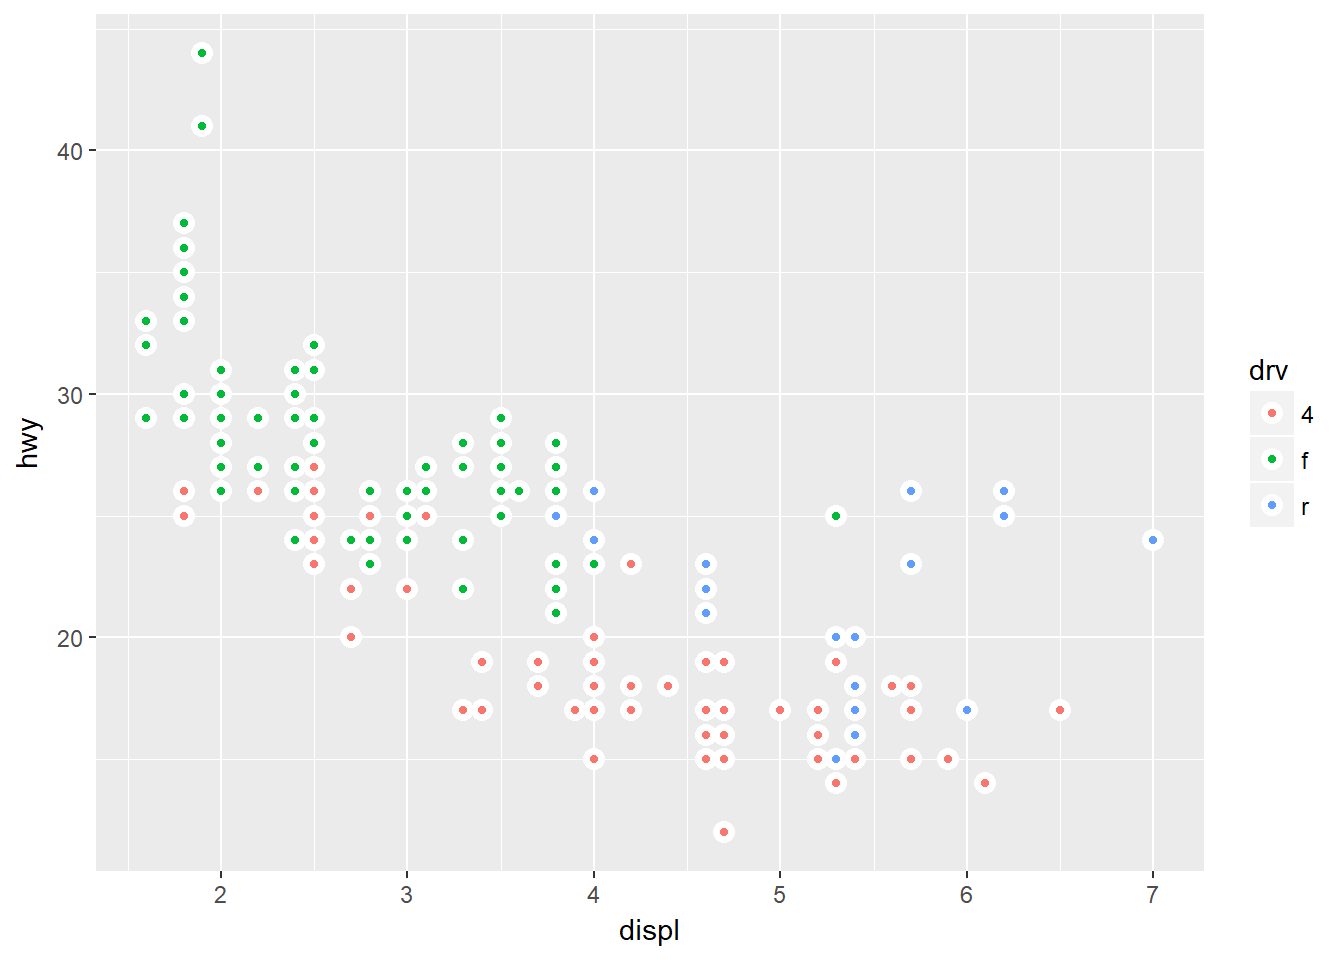
\includegraphics{R4DS_bookdown_files/figure-latex/unnamed-chunk-33-1.pdf}

\subsection{Statistical
transformations}\label{statistical-transformations}

\subsubsection{Exercises}\label{exercises-4}

\emph{1 - What is the default geom associated with
\texttt{stat\_summary()}? How could you rewrite the previous plot to use
that geom function instead of the stat function?}

The default geom for \texttt{stat\_summary()} is
\texttt{geom\_pointrange()}. However, the default stat for
\texttt{geom\_pointrage()} is \texttt{stat\_identity()}, meaning that
the medians, mins and maxes must be computed first. The plot can be
recreated with the following code:

\begin{Shaded}
\begin{Highlighting}[]
\NormalTok{diamonds }\OperatorTok\StringTok{ }\KeywordTok{group_by}\NormalTok{(cut) }\OperatorTok\StringTok{ }\KeywordTok{summarize}\NormalTok{(}\DataTypeTok{median_y =} \KeywordTok{median}\NormalTok{(depth),}
                                         \DataTypeTok{min_y =} \KeywordTok{min}\NormalTok{(depth),}
                                         \DataTypeTok{max_y =} \KeywordTok{max}\NormalTok{(depth)) }\OperatorTok
\StringTok{  }\KeywordTok{ggplot}\NormalTok{() }\OperatorTok{+}
\StringTok{  }\KeywordTok{geom_pointrange}\NormalTok{(}\DataTypeTok{mapping =} \KeywordTok{aes}\NormalTok{(}\DataTypeTok{x =}\NormalTok{ cut, }\DataTypeTok{y =}\NormalTok{ median_y, }\DataTypeTok{ymin =}\NormalTok{ min_y, }\DataTypeTok{ymax =}\NormalTok{ max_y)) }\OperatorTok{+}
\StringTok{  }\KeywordTok{labs}\NormalTok{(}\DataTypeTok{y =} \StringTok{'depth'}\NormalTok{)}
\end{Highlighting}
\end{Shaded}

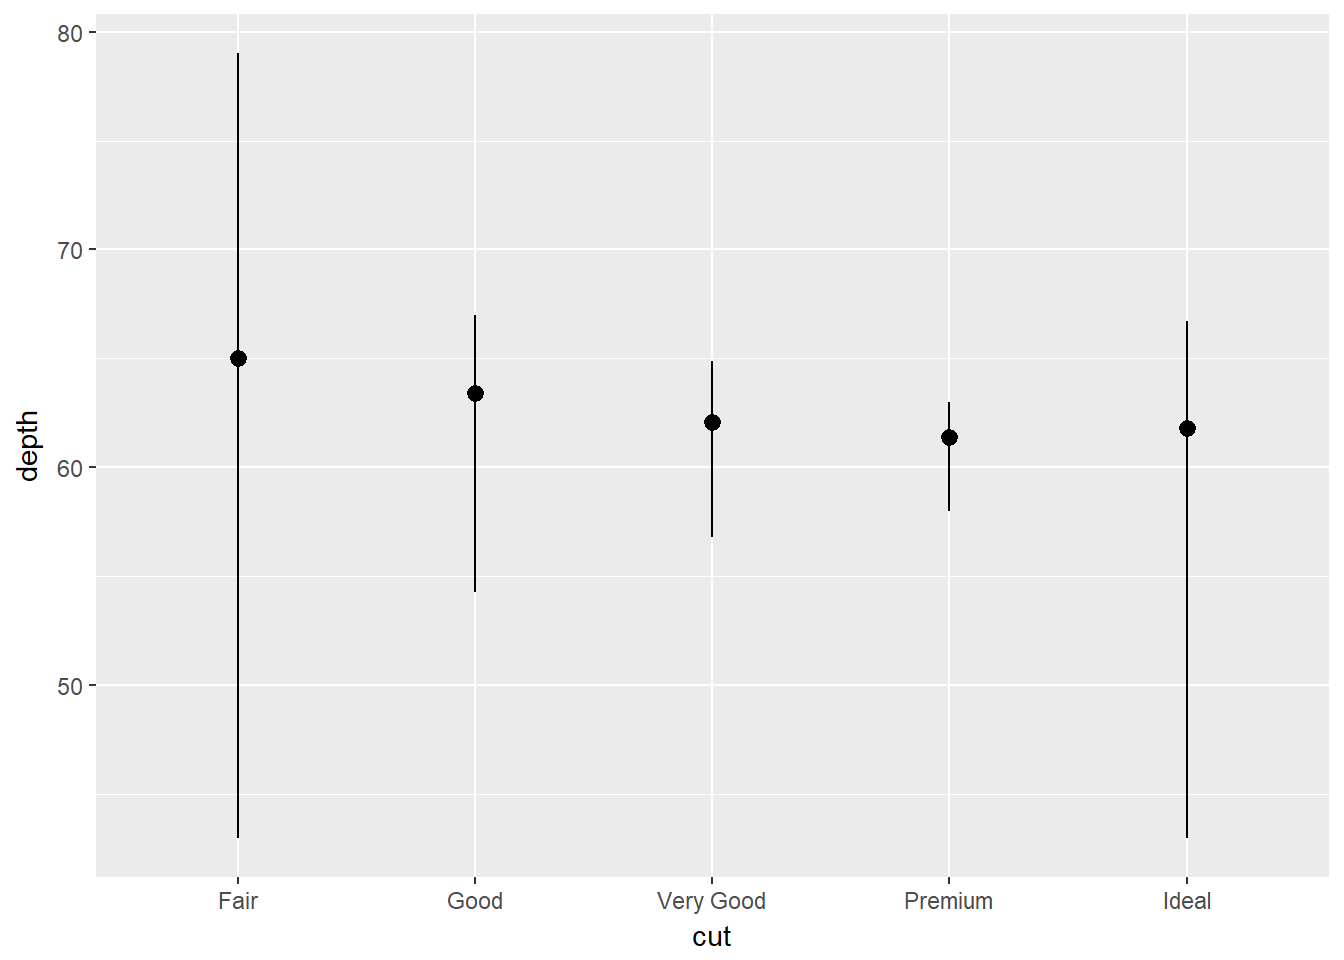
\includegraphics{R4DS_bookdown_files/figure-latex/unnamed-chunk-34-1.pdf}

\emph{2 - What does \texttt{geom\_col()} do? How is it different to
\texttt{geom\_bar()}?}

Both \texttt{geom\_col()} and \texttt{geom\_bar()} create bar charts.
The major difference is that for \texttt{geom\_bar()}, the default stat
is \texttt{stat\_count()}. It performs statistical transformation by
counting the frequencies in each group and then makes the height of the
bars proportional to the frequencies. For example:

\begin{Shaded}
\begin{Highlighting}[]
\KeywordTok{ggplot}\NormalTok{(}\DataTypeTok{data =}\NormalTok{ diamonds) }\OperatorTok{+}
\StringTok{  }\KeywordTok{geom_bar}\NormalTok{(}\KeywordTok{aes}\NormalTok{(}\DataTypeTok{x =}\NormalTok{ cut))}
\end{Highlighting}
\end{Shaded}

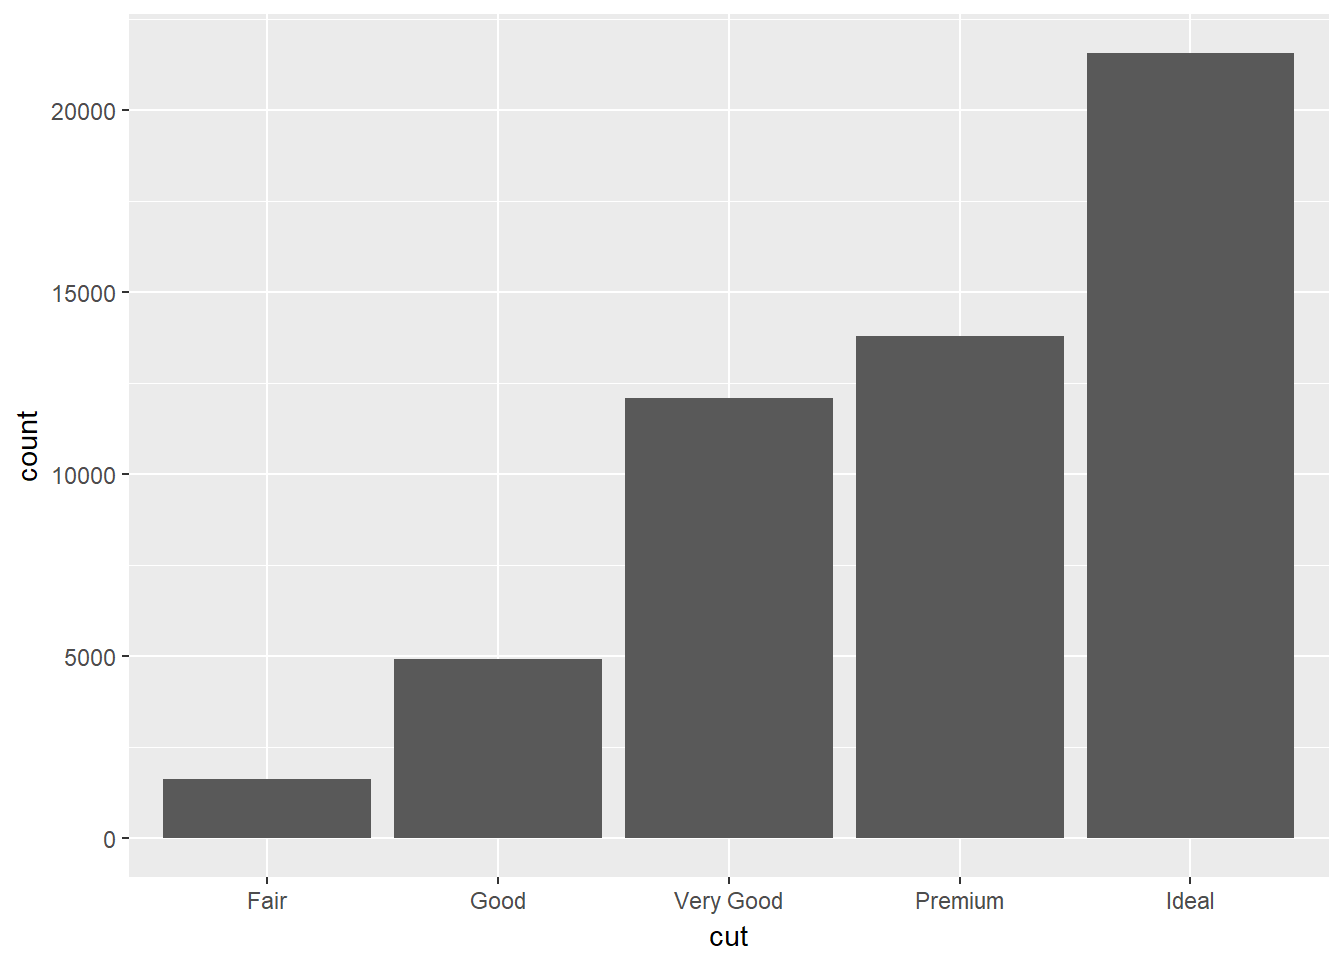
\includegraphics{R4DS_bookdown_files/figure-latex/unnamed-chunk-35-1.pdf}

Whereas for \texttt{geom\_col()}, the default stat is
\texttt{geom\_identity()}. The heights of the bars represent the values
in the data. To recreate the above bar chart using \texttt{geom\_col()},
we must first calculate the frequncies manually:

\begin{Shaded}
\begin{Highlighting}[]
\NormalTok{diamonds }\OperatorTok\StringTok{ }\KeywordTok{group_by}\NormalTok{(cut) }\OperatorTok\StringTok{ }\KeywordTok{summarise}\NormalTok{(}\DataTypeTok{count =} \KeywordTok{n}\NormalTok{()) }\OperatorTok
\StringTok{  }\KeywordTok{ggplot}\NormalTok{() }\OperatorTok{+}
\StringTok{  }\KeywordTok{geom_col}\NormalTok{(}\DataTypeTok{mapping =} \KeywordTok{aes}\NormalTok{(}\DataTypeTok{x =}\NormalTok{ cut, }\DataTypeTok{y =}\NormalTok{ count))}
\end{Highlighting}
\end{Shaded}

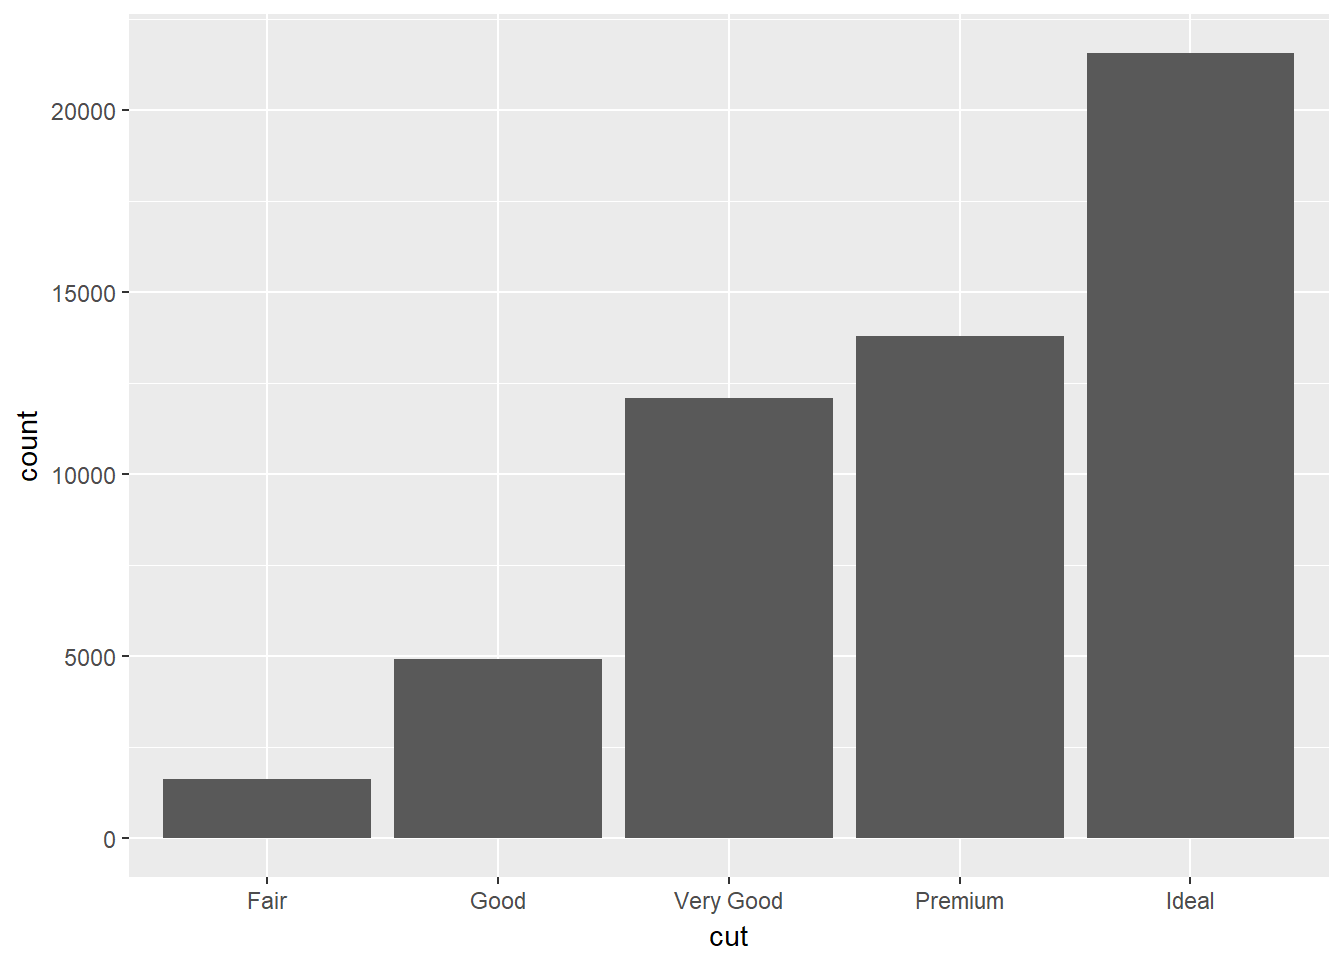
\includegraphics{R4DS_bookdown_files/figure-latex/unnamed-chunk-36-1.pdf}

\emph{3 - Most geoms and stats come in pairs that are almost always used
in concert. Read through the documentation and make a list of all the
pairs. What do they have in common?}

The complete list of geoms and stats can be found in the
\href{http://ggplot2.tidyverse.org/reference/}{documentation}.

\emph{4 - What variables does \texttt{stat\_smooth()} compute? What
parameters control its behaviour?}

The \texttt{method} argument defines the smoothing method and the
variables to compute. The arguments \texttt{n}, \texttt{span},
\texttt{fullrange}, and \texttt{level} controls its behaviour.

\emph{5 - In our proportion bar chart, we need to set
\texttt{group\ =\ 1}. Why? In other words what is the problem with these
two graphs?}

By default, \texttt{geom\_bar()} counts the number of occurances in each
level of the variable. However, if we want to display the proportions
instead of counts, \texttt{geom\_bar()} will treat the groups of the
variable separately. Since all diamonds in `Fair' are `Fair', and all
diamonds in `Ideal' are `Idea', etc., the proportions will always sum up
to 1 for each group by default.

\begin{Shaded}
\begin{Highlighting}[]
\KeywordTok{ggplot}\NormalTok{(}\DataTypeTok{data =}\NormalTok{ diamonds) }\OperatorTok{+}\StringTok{ }
\StringTok{  }\KeywordTok{geom_bar}\NormalTok{(}\DataTypeTok{mapping =} \KeywordTok{aes}\NormalTok{(}\DataTypeTok{x =}\NormalTok{ cut, }\DataTypeTok{y =}\NormalTok{ ..prop..))}
\end{Highlighting}
\end{Shaded}

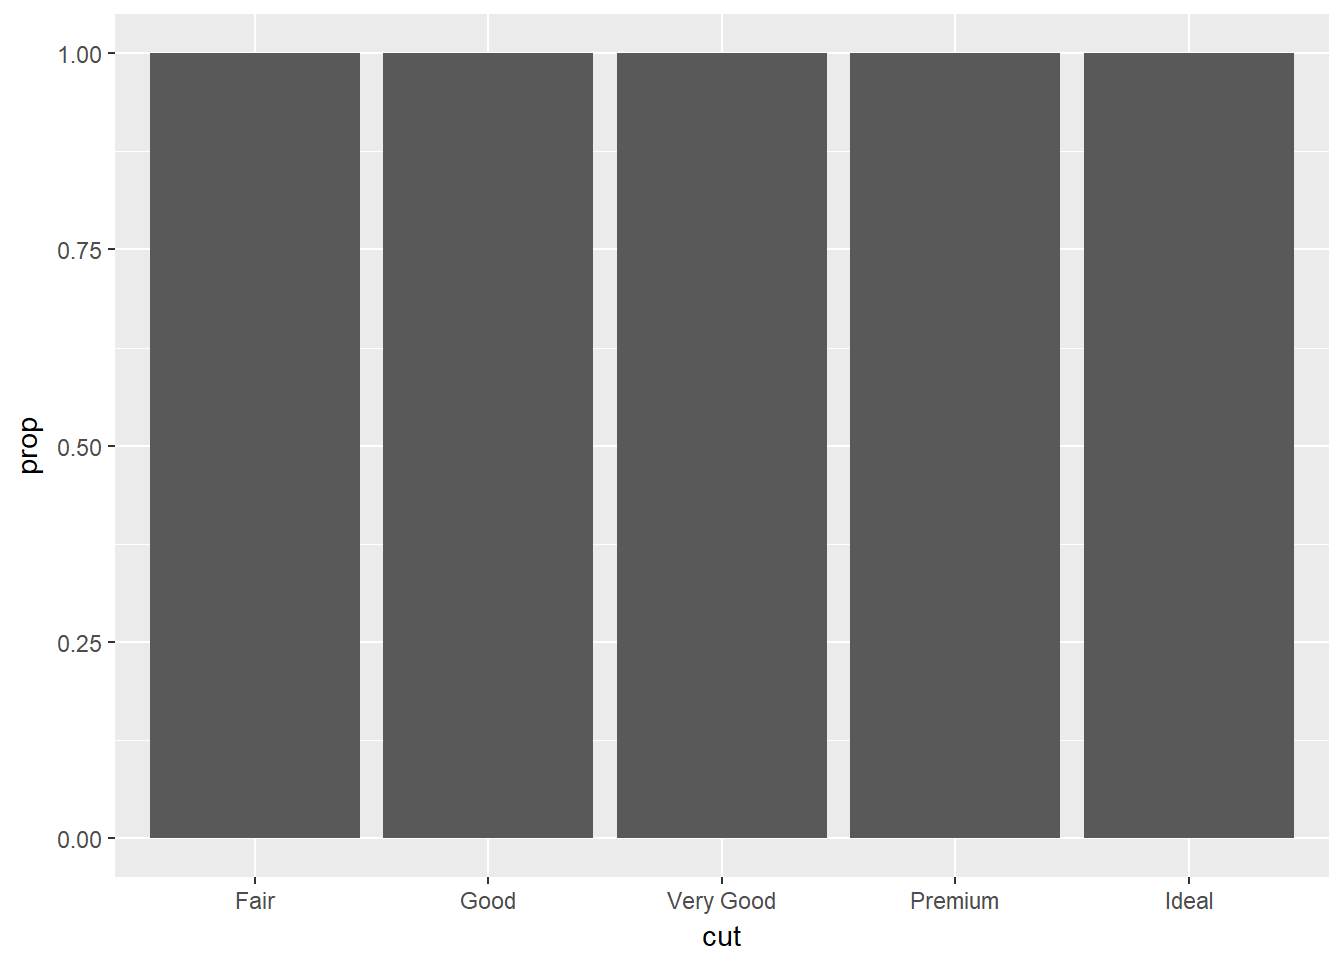
\includegraphics{R4DS_bookdown_files/figure-latex/unnamed-chunk-37-1.pdf}

To override this behavior and actually show the correct proportions
relatively to the overall counts, we can specify \texttt{group\ =\ 1}:

\begin{Shaded}
\begin{Highlighting}[]
\KeywordTok{ggplot}\NormalTok{(}\DataTypeTok{data =}\NormalTok{ diamonds) }\OperatorTok{+}\StringTok{ }
\StringTok{  }\KeywordTok{geom_bar}\NormalTok{(}\DataTypeTok{mapping =} \KeywordTok{aes}\NormalTok{(}\DataTypeTok{x =}\NormalTok{ cut, }\DataTypeTok{y =}\NormalTok{ ..prop.., }\DataTypeTok{group =} \DecValTok{1}\NormalTok{))}
\end{Highlighting}
\end{Shaded}

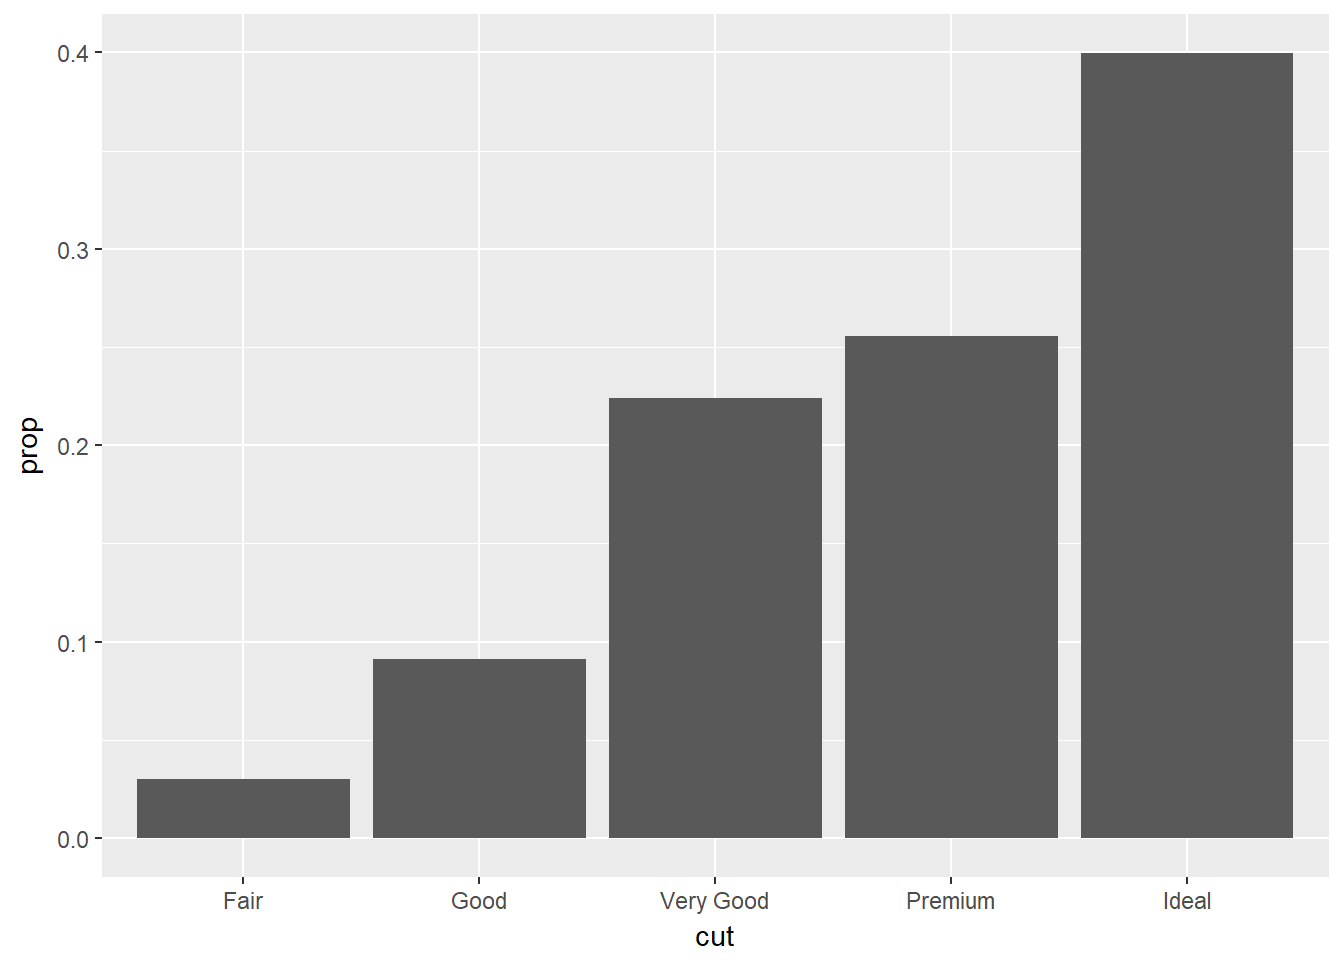
\includegraphics{R4DS_bookdown_files/figure-latex/unnamed-chunk-38-1.pdf}

Similarly in the second plot, \texttt{geom\_bar} first separates the cut
levels, then looks each color in each level indiviudally. Since all
color `D' in `Fair' are color `D', and all color `E' in `Good' are color
`E', etc., the proportion for each color in each cut level is always 1.
There are 7 colors in each cut level, so the proportions all sum up to
7.

\begin{Shaded}
\begin{Highlighting}[]
\KeywordTok{ggplot}\NormalTok{(}\DataTypeTok{data =}\NormalTok{ diamonds) }\OperatorTok{+}\StringTok{ }
\StringTok{  }\KeywordTok{geom_bar}\NormalTok{(}\DataTypeTok{mapping =} \KeywordTok{aes}\NormalTok{(}\DataTypeTok{x =}\NormalTok{ cut, }\DataTypeTok{fill =}\NormalTok{ color, }\DataTypeTok{y =}\NormalTok{ ..prop..))}
\end{Highlighting}
\end{Shaded}

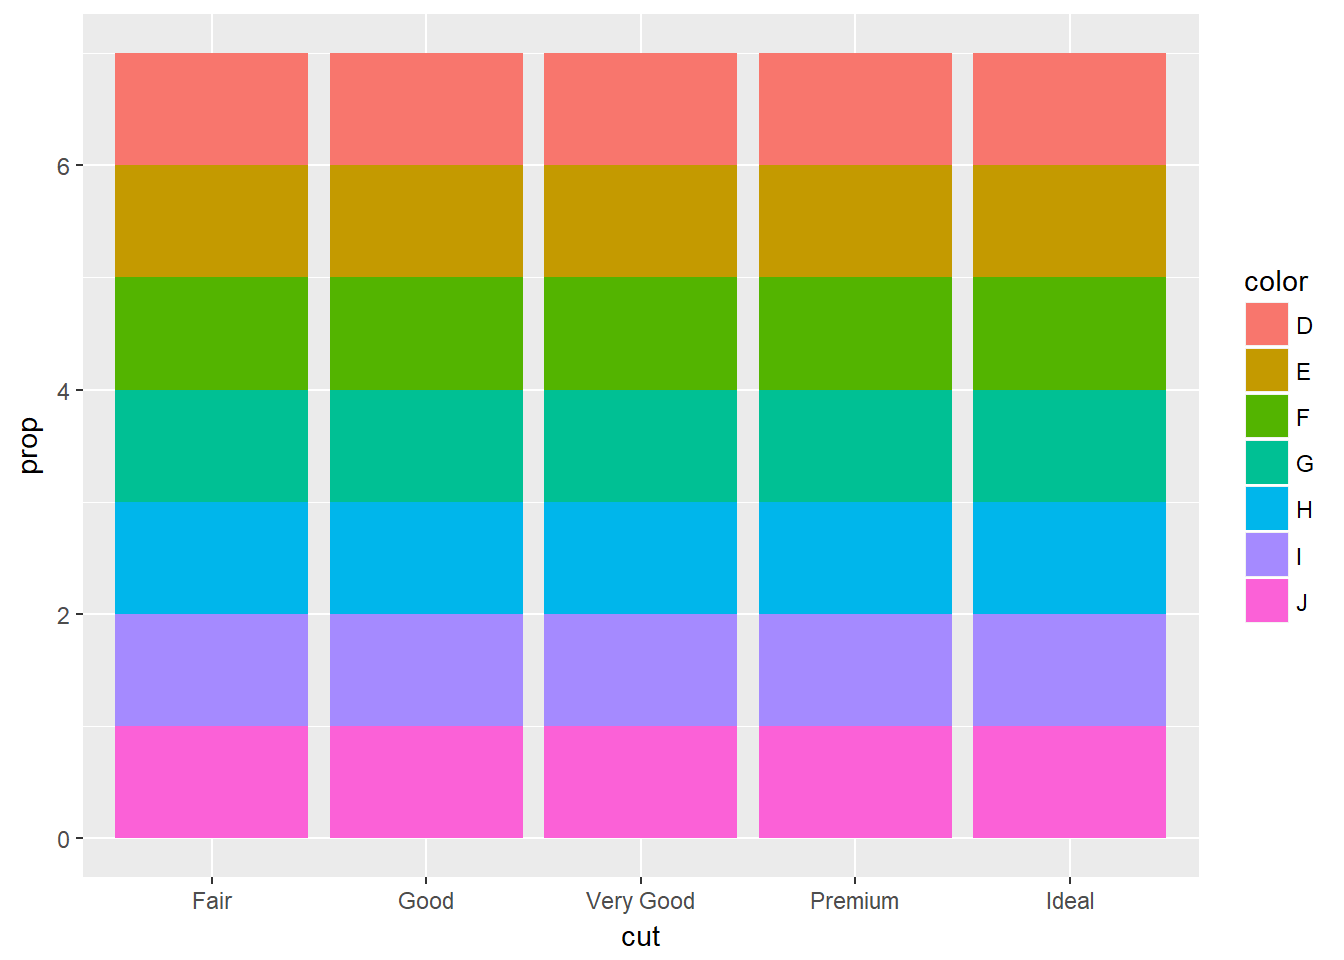
\includegraphics{R4DS_bookdown_files/figure-latex/unnamed-chunk-39-1.pdf}

To override this behavior, this time we can include
\texttt{group\ =\ color}.

\begin{Shaded}
\begin{Highlighting}[]
\KeywordTok{ggplot}\NormalTok{(}\DataTypeTok{data =}\NormalTok{ diamonds) }\OperatorTok{+}\StringTok{ }
\StringTok{  }\KeywordTok{geom_bar}\NormalTok{(}\DataTypeTok{mapping =} \KeywordTok{aes}\NormalTok{(}\DataTypeTok{x =}\NormalTok{ cut, }\DataTypeTok{fill =}\NormalTok{ color, }\DataTypeTok{y =}\NormalTok{ ..prop.., }\DataTypeTok{group =}\NormalTok{ color))}
\end{Highlighting}
\end{Shaded}

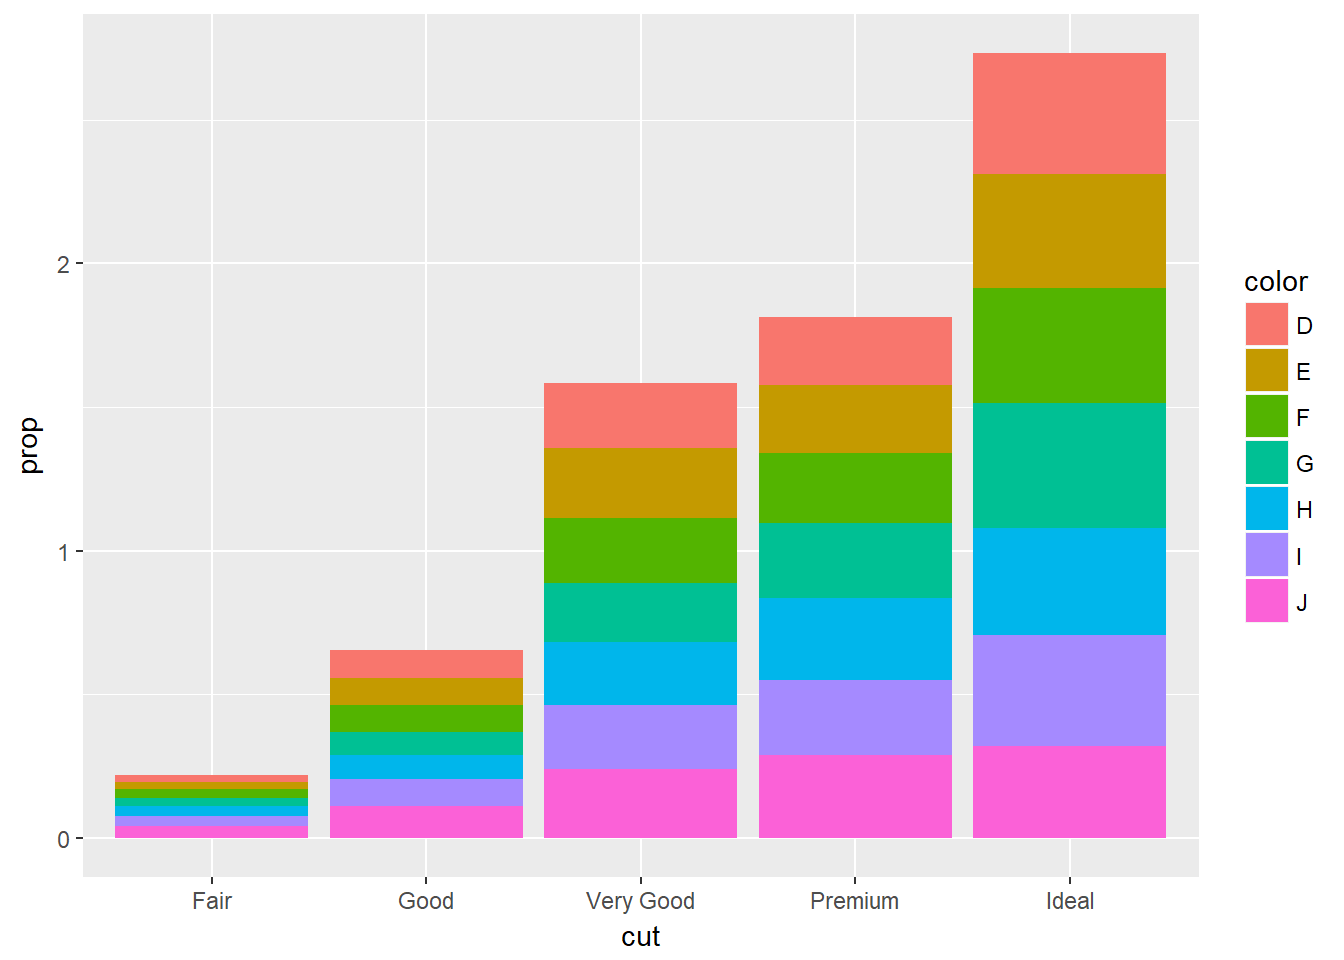
\includegraphics{R4DS_bookdown_files/figure-latex/unnamed-chunk-40-1.pdf}

Note that although visually it looks correct, the proportions are still
only relatively to the respective colors. For example, the sum of the
proportions of color `D' is 1, and since there are 7 colors, the sum of
the total height of the 5 bars is 7. Again to remedy this, instead of a
stacked bar chart, we can modify the \texttt{position} argument to
\texttt{dodge}:

\begin{Shaded}
\begin{Highlighting}[]
\KeywordTok{ggplot}\NormalTok{(}\DataTypeTok{data =}\NormalTok{ diamonds) }\OperatorTok{+}\StringTok{ }
\StringTok{  }\KeywordTok{geom_bar}\NormalTok{(}\DataTypeTok{mapping =} \KeywordTok{aes}\NormalTok{(}\DataTypeTok{x =}\NormalTok{ cut, }\DataTypeTok{fill =}\NormalTok{ color, }\DataTypeTok{y =}\NormalTok{ ..prop.., }\DataTypeTok{group =}\NormalTok{ color),}
           \DataTypeTok{position =} \StringTok{'dodge'}\NormalTok{)}
\end{Highlighting}
\end{Shaded}

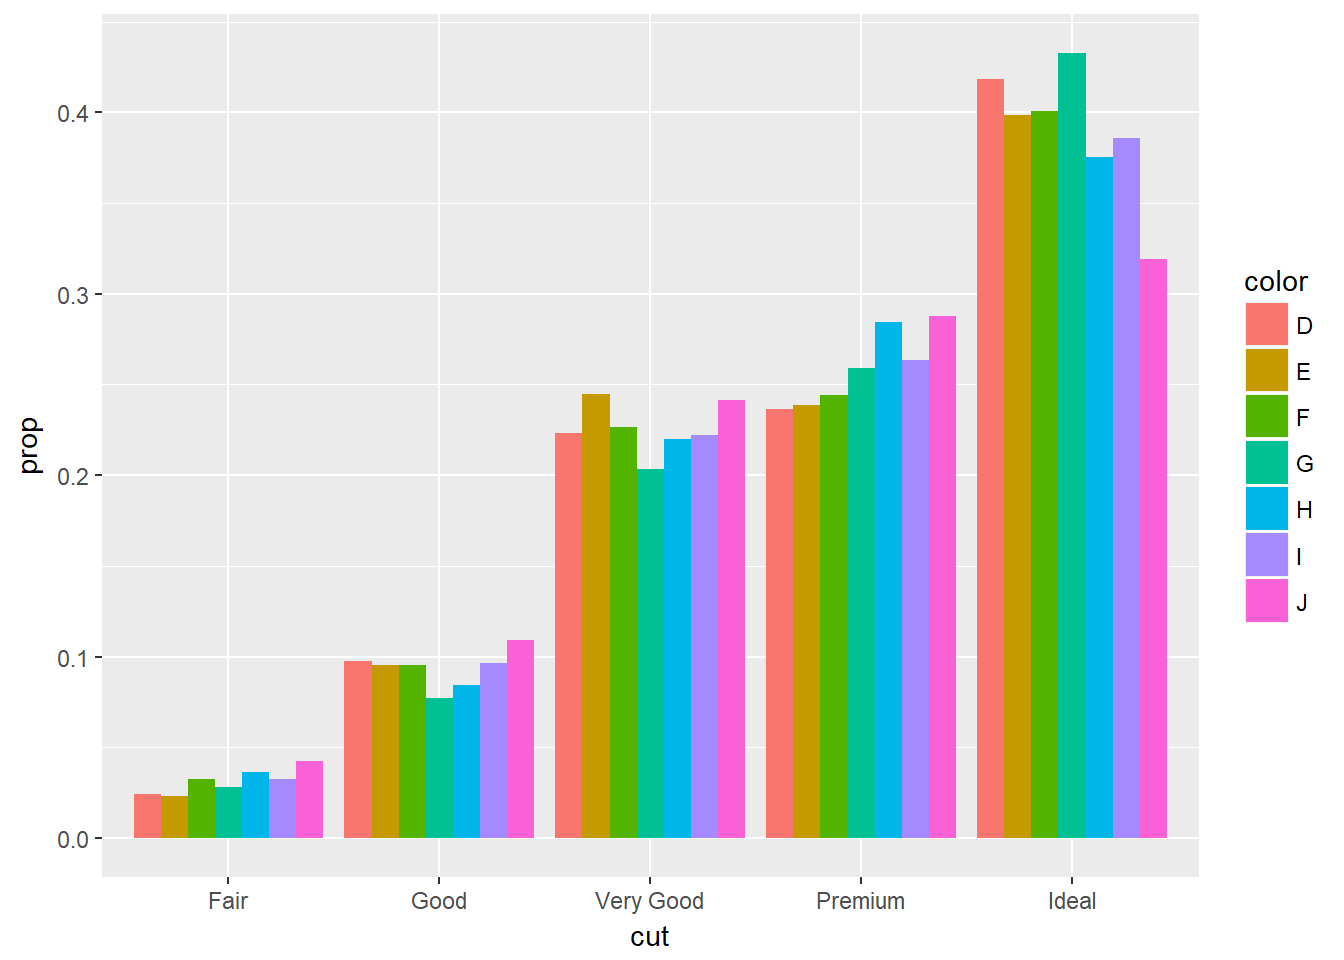
\includegraphics{R4DS_bookdown_files/figure-latex/unnamed-chunk-41-1.pdf}

\subsection{Position adjustments}\label{position-adjustments}

\subsubsection{Exercises}\label{exercises-5}

\emph{1 - What is the problem with this plot? How could you improve it?}

\begin{Shaded}
\begin{Highlighting}[]
\KeywordTok{ggplot}\NormalTok{(}\DataTypeTok{data =}\NormalTok{ mpg, }\DataTypeTok{mapping =} \KeywordTok{aes}\NormalTok{(}\DataTypeTok{x =}\NormalTok{ cty, }\DataTypeTok{y =}\NormalTok{ hwy)) }\OperatorTok{+}\StringTok{ }
\StringTok{  }\KeywordTok{geom_point}\NormalTok{()}
\end{Highlighting}
\end{Shaded}

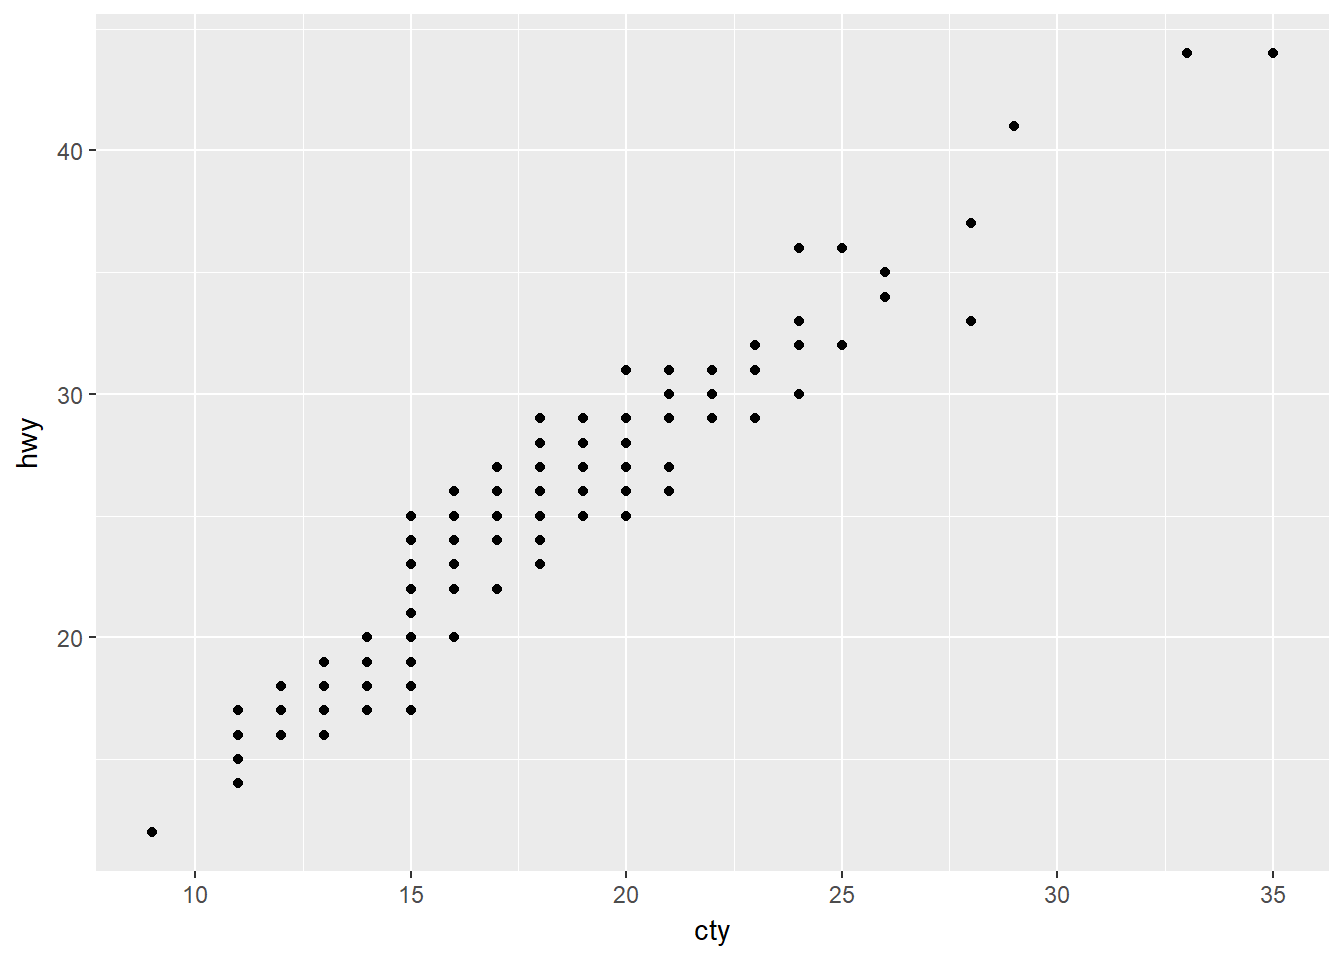
\includegraphics{R4DS_bookdown_files/figure-latex/unnamed-chunk-42-1.pdf}

The problem with this plot is that since there are many observations
with the same values of \texttt{cty} and \texttt{hwy}, many data points
overlap with each other and it fails to show where the mass of the data
is. We can use \texttt{geom\_jitter()} instead:

\begin{Shaded}
\begin{Highlighting}[]
\KeywordTok{ggplot}\NormalTok{(}\DataTypeTok{data =}\NormalTok{ mpg, }\DataTypeTok{mapping =} \KeywordTok{aes}\NormalTok{(}\DataTypeTok{x =}\NormalTok{ cty, }\DataTypeTok{y =}\NormalTok{ hwy)) }\OperatorTok{+}\StringTok{ }
\StringTok{  }\KeywordTok{geom_jitter}\NormalTok{()}
\end{Highlighting}
\end{Shaded}

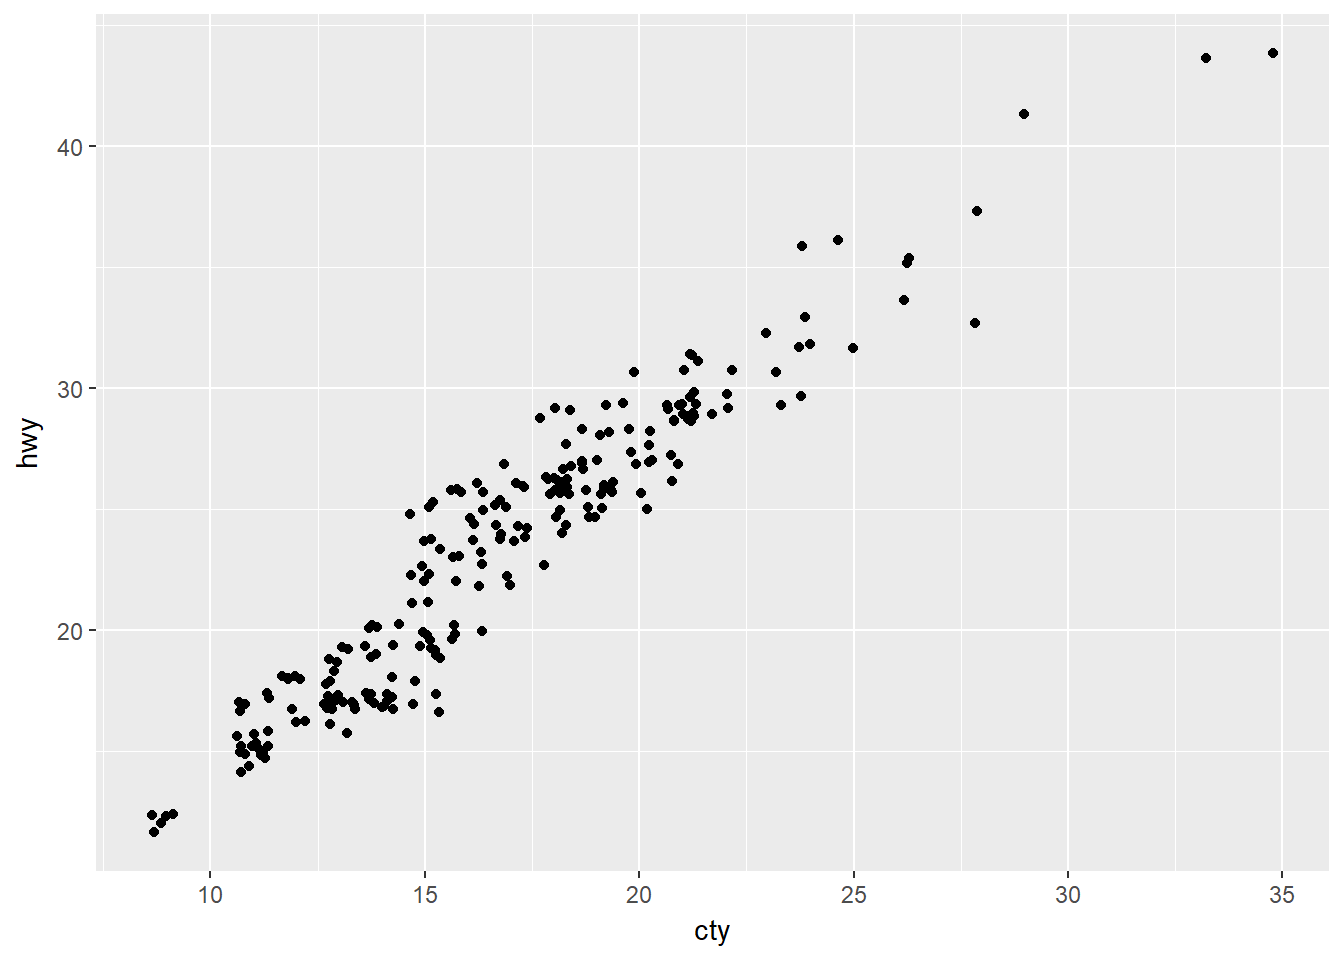
\includegraphics{R4DS_bookdown_files/figure-latex/unnamed-chunk-43-1.pdf}

\texttt{geom\_jitter} is able to display where the data points are
concentrated by sacrificing a little bit of statistically accuracy.

\emph{2 - What parameters to `\texttt{geom\_jitter()} control the amount
of jittering?}

The amount of jittering can be controlled by arguments \texttt{width}
and \texttt{height} in \texttt{geom\_jitter()}.

\emph{3 - Compare and contrast geom\_jitter() with geom\_count()}

Both \texttt{geom\_jitter()} and \texttt{geom\_count()} can better
represent the data when there are many overlapping points and show where
the mass of the data is. \texttt{geom\_jitter()} achieves this by
slightly moving the overlapping points vertically and horizontally,
sacrificing statistical accuracy while being more clearly in showing the
overlapping points. \texttt{geom\_count()} counts the overlapping
points, and maps the counts to the size of the points instead.

\begin{Shaded}
\begin{Highlighting}[]
\KeywordTok{ggplot}\NormalTok{(}\DataTypeTok{data =}\NormalTok{ mpg, }\DataTypeTok{mapping =} \KeywordTok{aes}\NormalTok{(}\DataTypeTok{x =}\NormalTok{ cty, }\DataTypeTok{y =}\NormalTok{ hwy)) }\OperatorTok{+}\StringTok{ }
\StringTok{  }\KeywordTok{geom_count}\NormalTok{()}
\end{Highlighting}
\end{Shaded}

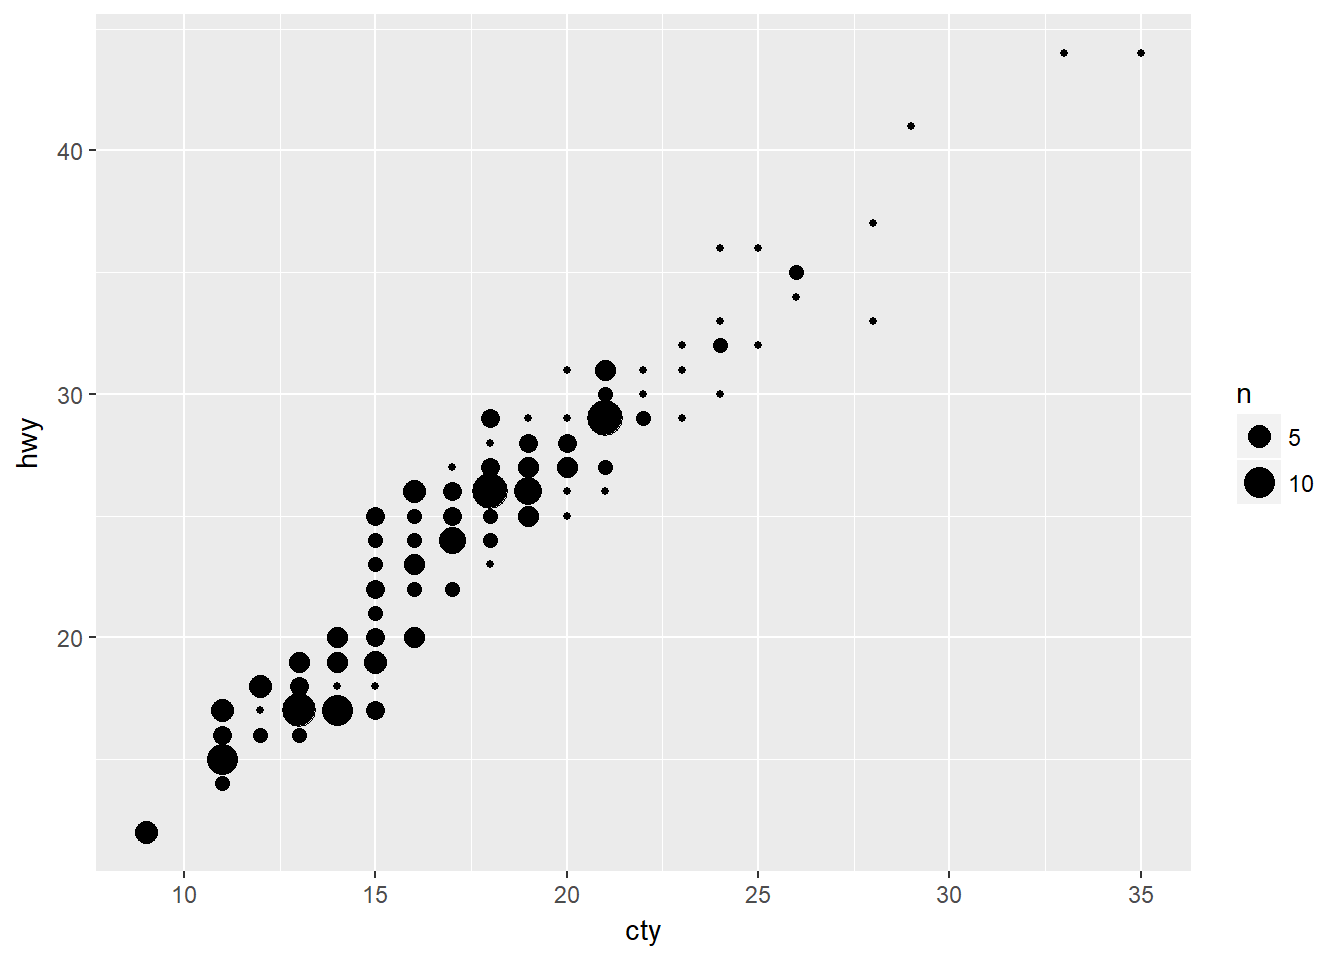
\includegraphics{R4DS_bookdown_files/figure-latex/unnamed-chunk-44-1.pdf}

\emph{4 - What's the default position adjustment for
\texttt{geom\_boxplot()}? Create a visualisation of the \texttt{mpg}
dataset that demonstrates it.}

The default positional adjustment is \texttt{dodge}.

\begin{Shaded}
\begin{Highlighting}[]
\KeywordTok{ggplot}\NormalTok{(}\DataTypeTok{data =}\NormalTok{ mpg) }\OperatorTok{+}
\StringTok{  }\KeywordTok{geom_boxplot}\NormalTok{(}\DataTypeTok{mapping =} \KeywordTok{aes}\NormalTok{(}\DataTypeTok{y =}\NormalTok{ displ, }\DataTypeTok{x =}\NormalTok{ drv, }\DataTypeTok{color =} \KeywordTok{factor}\NormalTok{(year)))}
\end{Highlighting}
\end{Shaded}

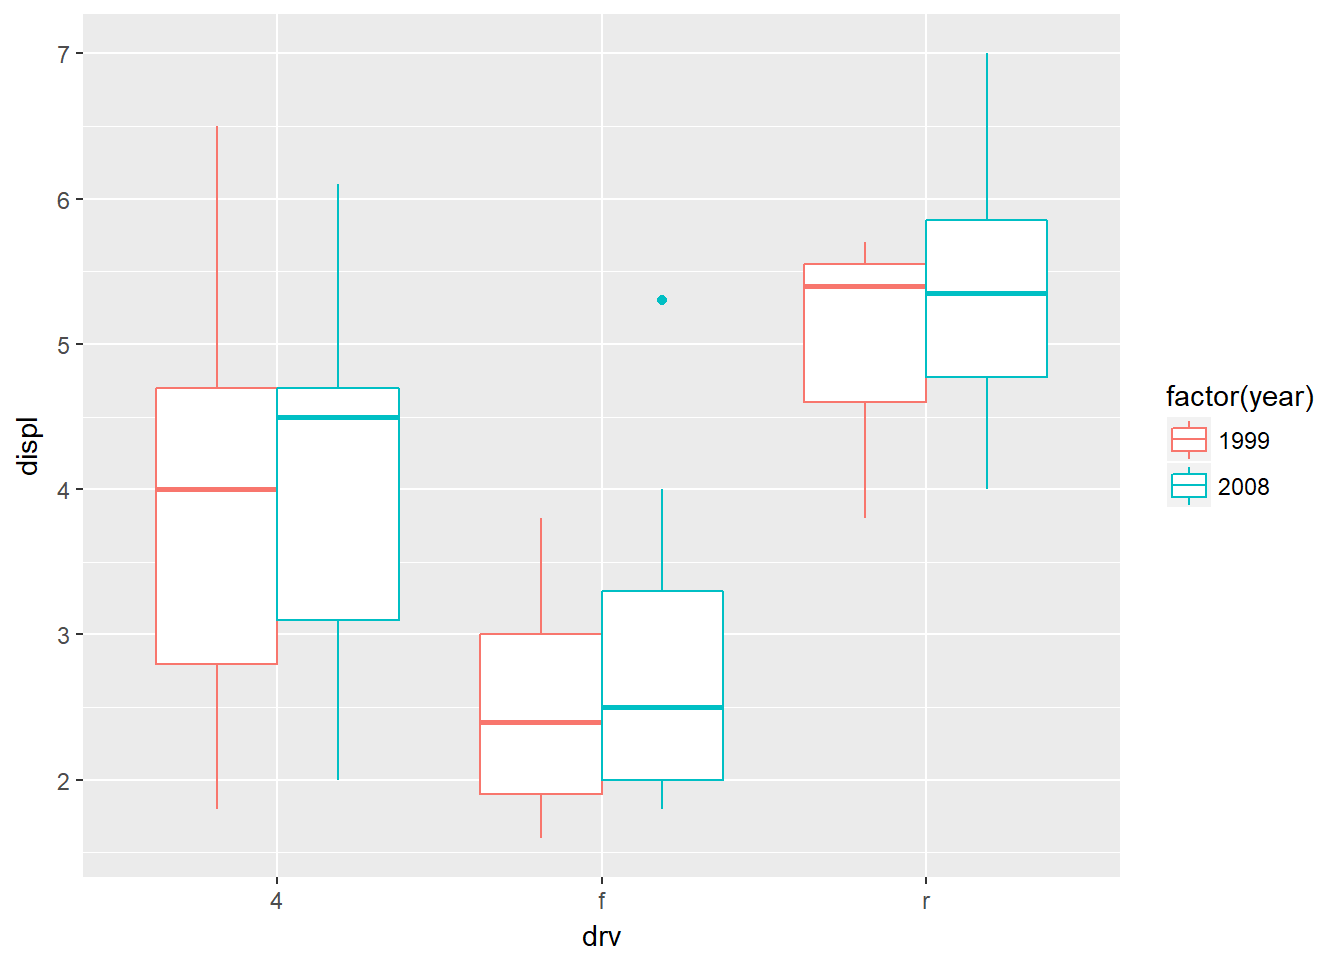
\includegraphics{R4DS_bookdown_files/figure-latex/unnamed-chunk-45-1.pdf}

\subsection{Coordinate systems}\label{coordinate-systems}

\subsubsection{Exercises}\label{exercises-6}

\emph{1 - Turn a stacked bar chart into a pie chart using
\texttt{coord\_polar()}}

Using the previous example in the chapter:

\begin{Shaded}
\begin{Highlighting}[]
\KeywordTok{ggplot}\NormalTok{(}\DataTypeTok{data =}\NormalTok{ diamonds) }\OperatorTok{+}\StringTok{ }
\StringTok{  }\KeywordTok{geom_bar}\NormalTok{(}\DataTypeTok{mapping =} \KeywordTok{aes}\NormalTok{(}\DataTypeTok{x =}\NormalTok{ cut, }\DataTypeTok{fill =}\NormalTok{ clarity)) }\OperatorTok{+}
\StringTok{  }\KeywordTok{coord_polar}\NormalTok{()}
\end{Highlighting}
\end{Shaded}

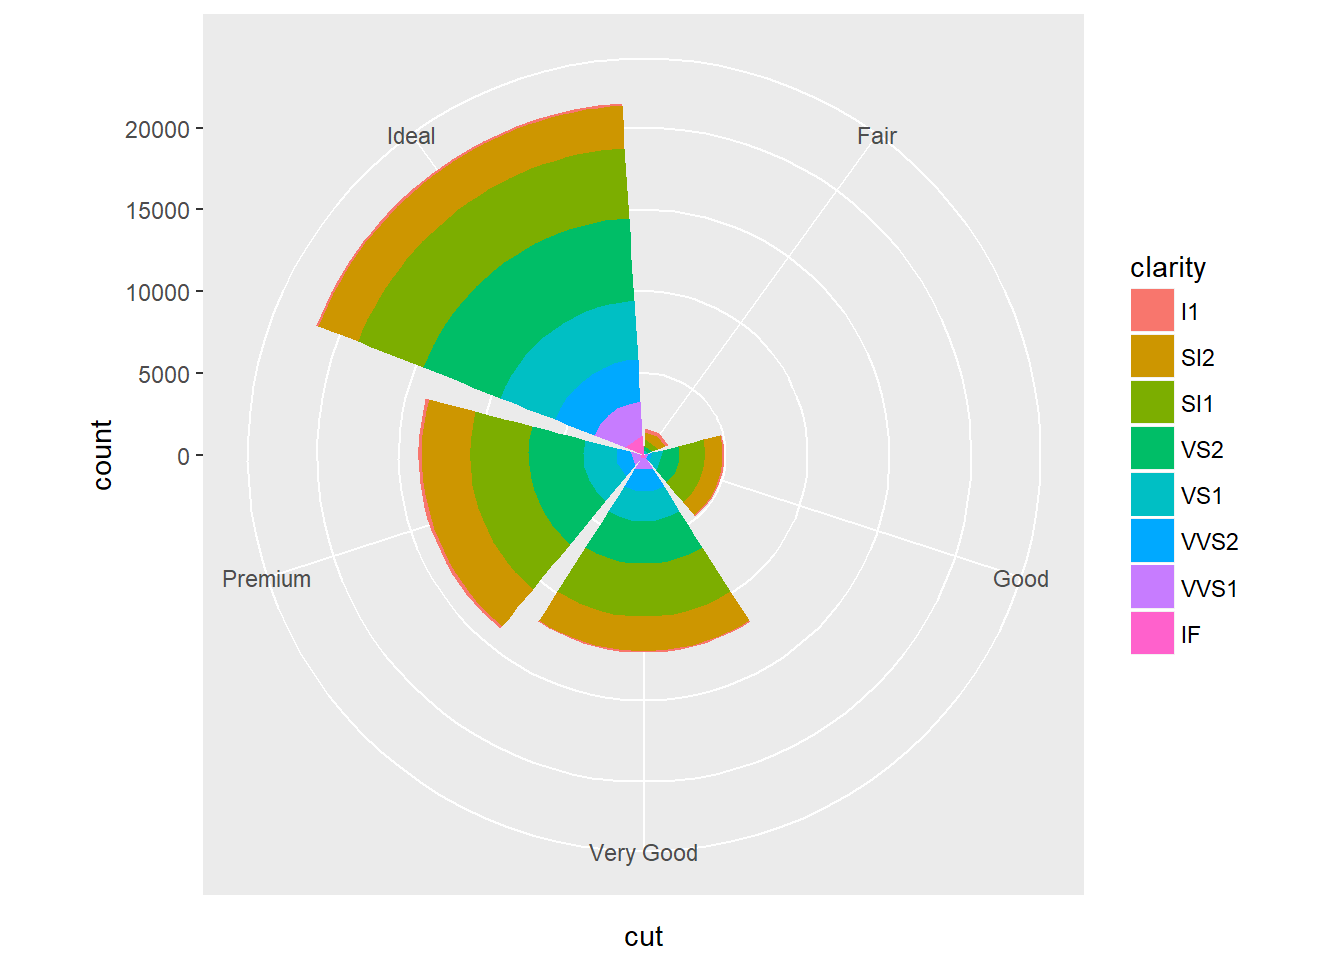
\includegraphics{R4DS_bookdown_files/figure-latex/unnamed-chunk-46-1.pdf}

In the above chart, the pies are angled by the x variable (cut). We can
angle the pies by the y variable using the arguement \texttt{theta}:

\begin{Shaded}
\begin{Highlighting}[]
\KeywordTok{ggplot}\NormalTok{(}\DataTypeTok{data =}\NormalTok{ diamonds) }\OperatorTok{+}\StringTok{ }
\StringTok{  }\KeywordTok{geom_bar}\NormalTok{(}\DataTypeTok{mapping =} \KeywordTok{aes}\NormalTok{(}\DataTypeTok{x =}\NormalTok{ cut, }\DataTypeTok{fill =}\NormalTok{ clarity)) }\OperatorTok{+}
\StringTok{  }\KeywordTok{coord_polar}\NormalTok{(}\DataTypeTok{theta =} \StringTok{"y"}\NormalTok{)}
\end{Highlighting}
\end{Shaded}

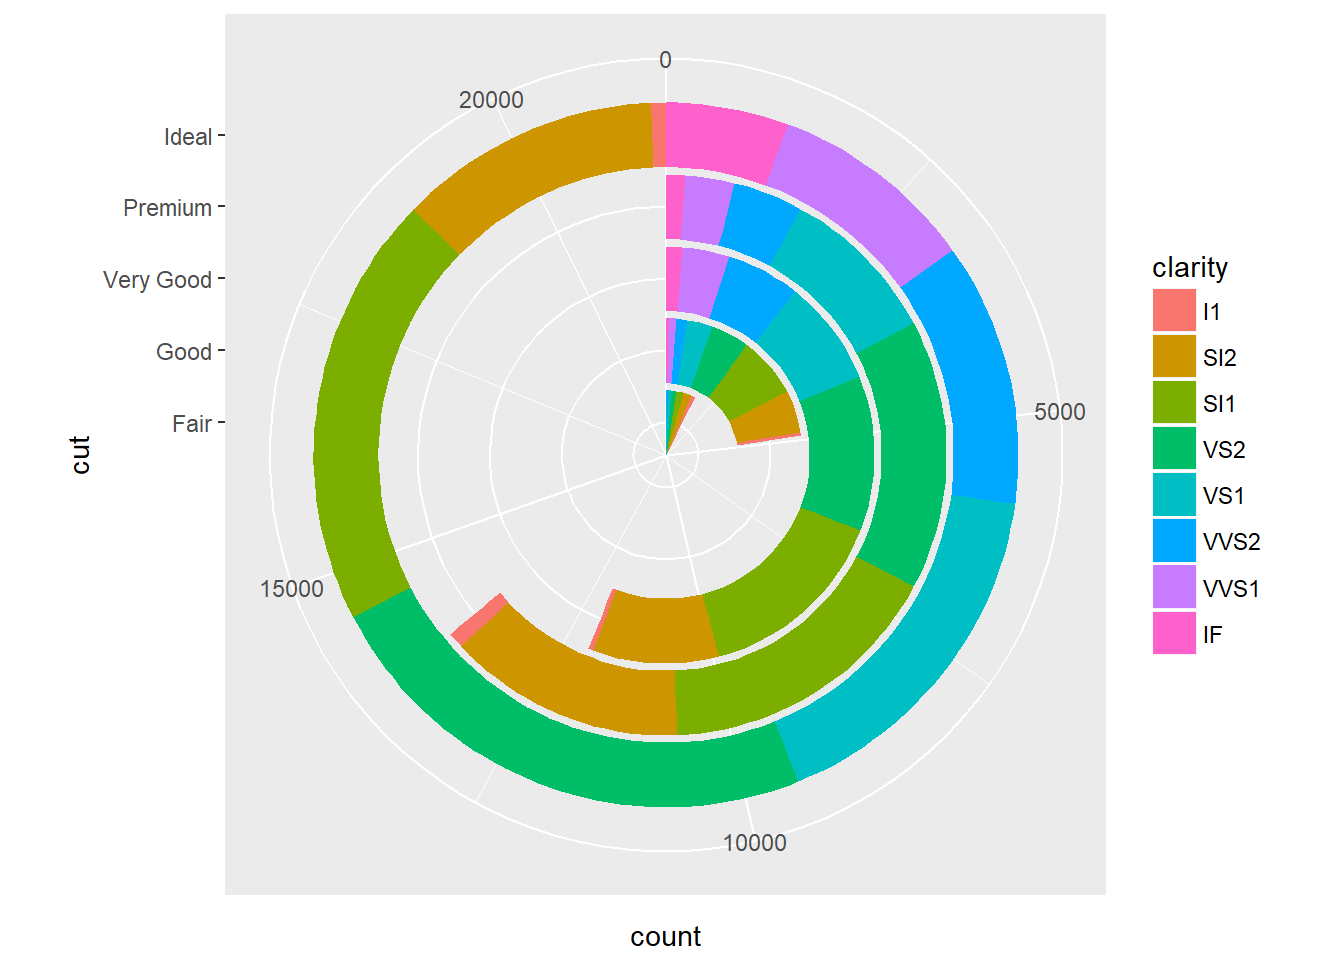
\includegraphics{R4DS_bookdown_files/figure-latex/unnamed-chunk-47-1.pdf}

\emph{2 - What does \texttt{labs()} do? Read the documentation.}

\texttt{labs()} allows us to modify ploy title, subtitle, axis title,
and legend title.

\emph{3 - What's the difference between coord\_quickmap() and
coord\_map()?}

Type \texttt{?coord\_map}, or read the description in the
\href{http://ggplot2.tidyverse.org/reference/coord_map.html}{reference}.

\emph{4 - What does the plot below tell you about the relationship
between city and highway mpg? Why is coord\_fixed() important? What does
geom\_abline() do?}

\begin{Shaded}
\begin{Highlighting}[]
\KeywordTok{ggplot}\NormalTok{(}\DataTypeTok{data =}\NormalTok{ mpg, }\DataTypeTok{mapping =} \KeywordTok{aes}\NormalTok{(}\DataTypeTok{x =}\NormalTok{ cty, }\DataTypeTok{y =}\NormalTok{ hwy)) }\OperatorTok{+}
\StringTok{  }\KeywordTok{geom_point}\NormalTok{() }\OperatorTok{+}\StringTok{ }
\StringTok{  }\KeywordTok{geom_abline}\NormalTok{() }\OperatorTok{+}
\StringTok{  }\KeywordTok{coord_fixed}\NormalTok{()}
\end{Highlighting}
\end{Shaded}

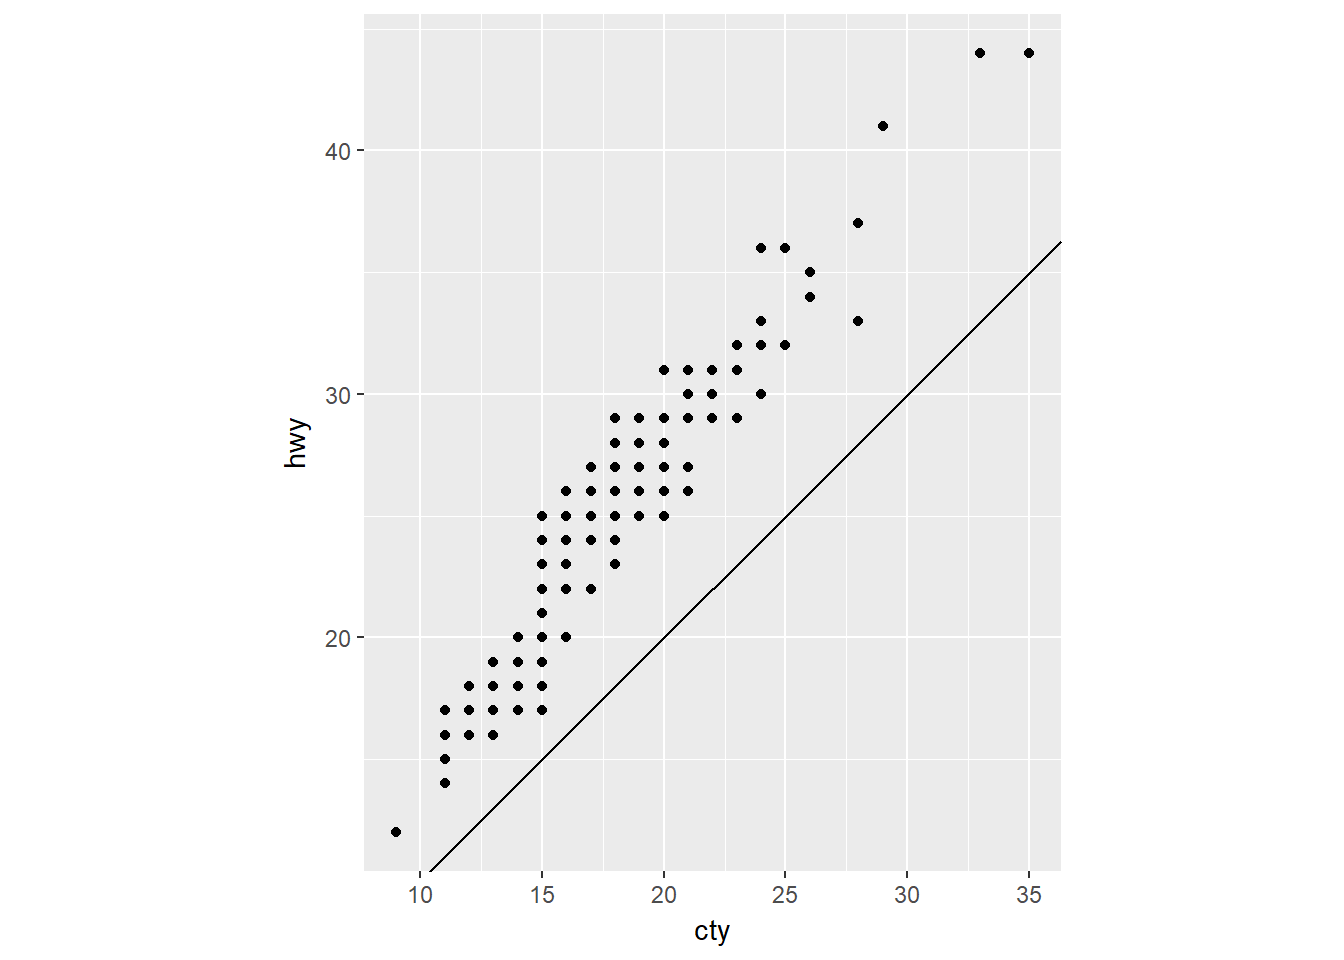
\includegraphics{R4DS_bookdown_files/figure-latex/unnamed-chunk-48-1.pdf}

The plot shows us that there is a positive linear trend between
\texttt{hwy} and \texttt{cty}, and the slope is approximately close 1,
meaning that a unit increase in \texttt{cty} is associated with a unit
increase in \texttt{hwy}.

\texttt{coord\_fixed} forces a specified aspect ratio between the
physical representation of the units on the axes. The ratio is 1 by
default. It is important to fix the aspect ratio in this case because
\texttt{hwy} and \texttt{cty} are measured in the same unit (miles per
gallon). Any other aspect ratios will give a visually incorrect
representation and might lead us to believe that one increasese at a
faster rate than the other.

\texttt{geom\_abline()} adds a diagonal reference line to the plot, thus
allows us the confidence earlier that the relationship is positively
linear and the slope is close to 1.

\subsection{The layered grammar of
graphics}\label{the-layered-grammar-of-graphics}

No exercises

\section{Workflow Basics}\label{workflow-basics}

\subsection{Coding basics}\label{coding-basics}

No exercises.

\subsection{What's in a name?}\label{whats-in-a-name}

No exercises.

\subsection{Calling functions}\label{calling-functions}

No exercises.

\subsection{Practice}\label{practice}

\emph{1 - Why does this code not work?}

\begin{Shaded}
\begin{Highlighting}[]
\NormalTok{my_variable <-}\StringTok{ }\DecValTok{10}
\NormalTok{my_varıable}
\CommentTok{#> Error in eval(expr, envir, enclos): object 'my_varıable' not found}
\end{Highlighting}
\end{Shaded}

\emph{Look carefully! (This may seem like an exercise in pointlessness,
but training your brain to notice even the tiniest difference will pay
off when programming.)}

The value \texttt{10} is assigned to \texttt{my\_variable}, not
\texttt{my\_varıable}. (Variables are named differently)

\emph{2 - Tweak each of the following R commands so that they run
correctly:}

\begin{Shaded}
\begin{Highlighting}[]
\KeywordTok{library}\NormalTok{(tidyverse)}

\KeywordTok{ggplot}\NormalTok{(}\DataTypeTok{dota =}\NormalTok{ mpg) }\OperatorTok{+}\StringTok{ }
\StringTok{  }\KeywordTok{geom_point}\NormalTok{(}\DataTypeTok{mapping =} \KeywordTok{aes}\NormalTok{(}\DataTypeTok{x =}\NormalTok{ displ, }\DataTypeTok{y =}\NormalTok{ hwy))}

\KeywordTok{fliter}\NormalTok{(mpg, }\DataTypeTok{cyl =} \DecValTok{8}\NormalTok{)}
\KeywordTok{filter}\NormalTok{(diamond, carat }\OperatorTok{>}\StringTok{ }\DecValTok{3}\NormalTok{)}
\end{Highlighting}
\end{Shaded}

Spelling is important. There are three typos in the above code: -
\texttt{dota} instead of \texttt{data} - the first \texttt{filter} is
misspelled as \texttt{fliter} - the dataset \texttt{diamond} should be
\texttt{diamonds}

The corrected code is shown below:

\begin{Shaded}
\begin{Highlighting}[]
\KeywordTok{library}\NormalTok{(tidyverse)}

\KeywordTok{ggplot}\NormalTok{(}\DataTypeTok{data =}\NormalTok{ mpg) }\OperatorTok{+}\StringTok{ }
\StringTok{  }\KeywordTok{geom_point}\NormalTok{(}\DataTypeTok{mapping =} \KeywordTok{aes}\NormalTok{(}\DataTypeTok{x =}\NormalTok{ displ, }\DataTypeTok{y =}\NormalTok{ hwy))}

\KeywordTok{filter}\NormalTok{(mpg, cyl }\OperatorTok{==}\StringTok{ }\DecValTok{8}\NormalTok{)}
\KeywordTok{filter}\NormalTok{(diamonds, carat }\OperatorTok{>}\StringTok{ }\DecValTok{3}\NormalTok{)}
\end{Highlighting}
\end{Shaded}

\emph{3 - Press Alt + Shift + K. What happens? How can you get to the
same place using the menus?}

The Keyboard Shortcut Quick Reference pops up. To get to the same place
using the menus, click Help on the menu bar, and it is under Keyboard
Shortcuts Help.

\section{Data transformation}\label{data-transformation}

\subsection{Introduction}\label{introduction-3}

No exercises.

\subsection{\texorpdfstring{Filter rows with
\texttt{filter()}}{Filter rows with filter()}}\label{filter-rows-with-filter}

\subsubsection{Exercises}\label{exercises-7}

\emph{1 - Find all flights that}

\emph{1. Had an arrival delay of two or more hours}

\begin{Shaded}
\begin{Highlighting}[]
\KeywordTok{library}\NormalTok{(tidyverse)}

\NormalTok{flights <-}\StringTok{ }\NormalTok{nycflights13}\OperatorTok{::}\NormalTok{flights}

\KeywordTok{filter}\NormalTok{(flights, arr_delay }\OperatorTok{>=}\StringTok{ }\DecValTok{120}\NormalTok{)}
\end{Highlighting}
\end{Shaded}

\begin{verbatim}
## # A tibble: 10,200 x 19
##     year month   day dep_time sched_dep_time dep_delay arr_time
##    <int> <int> <int>    <int>          <int>     <dbl>    <int>
##  1  2013     1     1      811            630     101       1047
##  2  2013     1     1      848           1835     853       1001
##  3  2013     1     1      957            733     144       1056
##  4  2013     1     1     1114            900     134       1447
##  5  2013     1     1     1505           1310     115       1638
##  6  2013     1     1     1525           1340     105       1831
##  7  2013     1     1     1549           1445      64.0     1912
##  8  2013     1     1     1558           1359     119       1718
##  9  2013     1     1     1732           1630      62.0     2028
## 10  2013     1     1     1803           1620     103       2008
## # ... with 10,190 more rows, and 12 more variables: sched_arr_time <int>,
## #   arr_delay <dbl>, carrier <chr>, flight <int>, tailnum <chr>,
## #   origin <chr>, dest <chr>, air_time <dbl>, distance <dbl>, hour <dbl>,
## #   minute <dbl>, time_hour <dttm>
\end{verbatim}

\emph{2. Flew to Houston (\texttt{IAH} or \texttt{HOU})}

\begin{Shaded}
\begin{Highlighting}[]
\KeywordTok{filter}\NormalTok{(flights, dest }\OperatorTok\StringTok{ }\KeywordTok{c}\NormalTok{(}\StringTok{'IAH'}\NormalTok{, }\StringTok{'HOU'}\NormalTok{))}
\end{Highlighting}
\end{Shaded}

\begin{verbatim}
## # A tibble: 9,313 x 19
##     year month   day dep_time sched_dep_time dep_delay arr_time
##    <int> <int> <int>    <int>          <int>     <dbl>    <int>
##  1  2013     1     1      517            515      2.00      830
##  2  2013     1     1      533            529      4.00      850
##  3  2013     1     1      623            627   -  4.00      933
##  4  2013     1     1      728            732   -  4.00     1041
##  5  2013     1     1      739            739      0        1104
##  6  2013     1     1      908            908      0        1228
##  7  2013     1     1     1028           1026      2.00     1350
##  8  2013     1     1     1044           1045   -  1.00     1352
##  9  2013     1     1     1114            900    134        1447
## 10  2013     1     1     1205           1200      5.00     1503
## # ... with 9,303 more rows, and 12 more variables: sched_arr_time <int>,
## #   arr_delay <dbl>, carrier <chr>, flight <int>, tailnum <chr>,
## #   origin <chr>, dest <chr>, air_time <dbl>, distance <dbl>, hour <dbl>,
## #   minute <dbl>, time_hour <dttm>
\end{verbatim}

\emph{3. Were operated by United, American, or Delta}

\begin{Shaded}
\begin{Highlighting}[]
\KeywordTok{filter}\NormalTok{(flights, carrier }\OperatorTok\StringTok{ }\KeywordTok{c}\NormalTok{(}\StringTok{'UA'}\NormalTok{,}\StringTok{'AA'}\NormalTok{,}\StringTok{'DL'}\NormalTok{))}
\end{Highlighting}
\end{Shaded}

\begin{verbatim}
## # A tibble: 139,504 x 19
##     year month   day dep_time sched_dep_time dep_delay arr_time
##    <int> <int> <int>    <int>          <int>     <dbl>    <int>
##  1  2013     1     1      517            515      2.00      830
##  2  2013     1     1      533            529      4.00      850
##  3  2013     1     1      542            540      2.00      923
##  4  2013     1     1      554            600     -6.00      812
##  5  2013     1     1      554            558     -4.00      740
##  6  2013     1     1      558            600     -2.00      753
##  7  2013     1     1      558            600     -2.00      924
##  8  2013     1     1      558            600     -2.00      923
##  9  2013     1     1      559            600     -1.00      941
## 10  2013     1     1      559            600     -1.00      854
## # ... with 139,494 more rows, and 12 more variables: sched_arr_time <int>,
## #   arr_delay <dbl>, carrier <chr>, flight <int>, tailnum <chr>,
## #   origin <chr>, dest <chr>, air_time <dbl>, distance <dbl>, hour <dbl>,
## #   minute <dbl>, time_hour <dttm>
\end{verbatim}

\emph{4. Departed in summer (July, August, and September)}

\begin{Shaded}
\begin{Highlighting}[]
\KeywordTok{filter}\NormalTok{(flights, month }\OperatorTok\StringTok{ }\KeywordTok{c}\NormalTok{(}\DecValTok{7}\NormalTok{,}\DecValTok{8}\NormalTok{,}\DecValTok{9}\NormalTok{))}
\end{Highlighting}
\end{Shaded}

\begin{verbatim}
## # A tibble: 86,326 x 19
##     year month   day dep_time sched_dep_time dep_delay arr_time
##    <int> <int> <int>    <int>          <int>     <dbl>    <int>
##  1  2013     7     1        1           2029    212         236
##  2  2013     7     1        2           2359      3.00      344
##  3  2013     7     1       29           2245    104         151
##  4  2013     7     1       43           2130    193         322
##  5  2013     7     1       44           2150    174         300
##  6  2013     7     1       46           2051    235         304
##  7  2013     7     1       48           2001    287         308
##  8  2013     7     1       58           2155    183         335
##  9  2013     7     1      100           2146    194         327
## 10  2013     7     1      100           2245    135         337
## # ... with 86,316 more rows, and 12 more variables: sched_arr_time <int>,
## #   arr_delay <dbl>, carrier <chr>, flight <int>, tailnum <chr>,
## #   origin <chr>, dest <chr>, air_time <dbl>, distance <dbl>, hour <dbl>,
## #   minute <dbl>, time_hour <dttm>
\end{verbatim}

\emph{5. Arrived more than two hours late, but didn't leave late}

\begin{Shaded}
\begin{Highlighting}[]
\KeywordTok{filter}\NormalTok{(flights, dep_delay }\OperatorTok{<=}\StringTok{ }\DecValTok{0}\NormalTok{, arr_delay }\OperatorTok{>=}\StringTok{ }\DecValTok{120}\NormalTok{)}
\end{Highlighting}
\end{Shaded}

\begin{verbatim}
## # A tibble: 29 x 19
##     year month   day dep_time sched_dep_time dep_delay arr_time
##    <int> <int> <int>    <int>          <int>     <dbl>    <int>
##  1  2013     1    27     1419           1420     -1.00     1754
##  2  2013    10     7     1350           1350      0        1736
##  3  2013    10     7     1357           1359     -2.00     1858
##  4  2013    10    16      657            700     -3.00     1258
##  5  2013    11     1      658            700     -2.00     1329
##  6  2013     3    18     1844           1847     -3.00       39
##  7  2013     4    17     1635           1640     -5.00     2049
##  8  2013     4    18      558            600     -2.00     1149
##  9  2013     4    18      655            700     -5.00     1213
## 10  2013     5    22     1827           1830     -3.00     2217
## # ... with 19 more rows, and 12 more variables: sched_arr_time <int>,
## #   arr_delay <dbl>, carrier <chr>, flight <int>, tailnum <chr>,
## #   origin <chr>, dest <chr>, air_time <dbl>, distance <dbl>, hour <dbl>,
## #   minute <dbl>, time_hour <dttm>
\end{verbatim}

\emph{6. Were delayed by at least an hour, but made up over 30 minutes
in flight}

\begin{Shaded}
\begin{Highlighting}[]
\KeywordTok{filter}\NormalTok{(flights, dep_delay }\OperatorTok{>=}\StringTok{ }\DecValTok{60}\NormalTok{, dep_delay }\OperatorTok{>}\StringTok{ }\NormalTok{arr_delay }\OperatorTok{+}\StringTok{ }\DecValTok{30}\NormalTok{)}
\end{Highlighting}
\end{Shaded}

\begin{verbatim}
## # A tibble: 1,844 x 19
##     year month   day dep_time sched_dep_time dep_delay arr_time
##    <int> <int> <int>    <int>          <int>     <dbl>    <int>
##  1  2013     1     1     2205           1720     285         46
##  2  2013     1     1     2326           2130     116        131
##  3  2013     1     3     1503           1221     162       1803
##  4  2013     1     3     1839           1700      99.0     2056
##  5  2013     1     3     1850           1745      65.0     2148
##  6  2013     1     3     1941           1759     102       2246
##  7  2013     1     3     1950           1845      65.0     2228
##  8  2013     1     3     2015           1915      60.0     2135
##  9  2013     1     3     2257           2000     177         45
## 10  2013     1     4     1917           1700     137       2135
## # ... with 1,834 more rows, and 12 more variables: sched_arr_time <int>,
## #   arr_delay <dbl>, carrier <chr>, flight <int>, tailnum <chr>,
## #   origin <chr>, dest <chr>, air_time <dbl>, distance <dbl>, hour <dbl>,
## #   minute <dbl>, time_hour <dttm>
\end{verbatim}

\emph{7. Departed between midnight and 6am (inclusive)}

\begin{Shaded}
\begin{Highlighting}[]
\KeywordTok{filter}\NormalTok{(flights, dep_time }\OperatorTok{>=}\StringTok{ }\DecValTok{0}\NormalTok{, dep_time }\OperatorTok{<=}\StringTok{ }\DecValTok{600}\NormalTok{)}
\end{Highlighting}
\end{Shaded}

\begin{verbatim}
## # A tibble: 9,344 x 19
##     year month   day dep_time sched_dep_time dep_delay arr_time
##    <int> <int> <int>    <int>          <int>     <dbl>    <int>
##  1  2013     1     1      517            515      2.00      830
##  2  2013     1     1      533            529      4.00      850
##  3  2013     1     1      542            540      2.00      923
##  4  2013     1     1      544            545     -1.00     1004
##  5  2013     1     1      554            600     -6.00      812
##  6  2013     1     1      554            558     -4.00      740
##  7  2013     1     1      555            600     -5.00      913
##  8  2013     1     1      557            600     -3.00      709
##  9  2013     1     1      557            600     -3.00      838
## 10  2013     1     1      558            600     -2.00      753
## # ... with 9,334 more rows, and 12 more variables: sched_arr_time <int>,
## #   arr_delay <dbl>, carrier <chr>, flight <int>, tailnum <chr>,
## #   origin <chr>, dest <chr>, air_time <dbl>, distance <dbl>, hour <dbl>,
## #   minute <dbl>, time_hour <dttm>
\end{verbatim}

\emph{2 - Another useful dplyr filtering helper is \texttt{between()}.
What does it do? Can you use it to simplify the code needed to answer
the previous challenges?}

\texttt{between()} is a shortcut for
\texttt{x\ \textgreater{}=\ left\ \&\ x\ \textless{}=\ right}. Part 7 of
the previous question can be rewritten as:

\begin{Shaded}
\begin{Highlighting}[]
\KeywordTok{filter}\NormalTok{(flights, }\KeywordTok{between}\NormalTok{(dep_time, }\DecValTok{0}\NormalTok{ , }\DecValTok{600}\NormalTok{))}
\end{Highlighting}
\end{Shaded}

\begin{verbatim}
## # A tibble: 9,344 x 19
##     year month   day dep_time sched_dep_time dep_delay arr_time
##    <int> <int> <int>    <int>          <int>     <dbl>    <int>
##  1  2013     1     1      517            515      2.00      830
##  2  2013     1     1      533            529      4.00      850
##  3  2013     1     1      542            540      2.00      923
##  4  2013     1     1      544            545     -1.00     1004
##  5  2013     1     1      554            600     -6.00      812
##  6  2013     1     1      554            558     -4.00      740
##  7  2013     1     1      555            600     -5.00      913
##  8  2013     1     1      557            600     -3.00      709
##  9  2013     1     1      557            600     -3.00      838
## 10  2013     1     1      558            600     -2.00      753
## # ... with 9,334 more rows, and 12 more variables: sched_arr_time <int>,
## #   arr_delay <dbl>, carrier <chr>, flight <int>, tailnum <chr>,
## #   origin <chr>, dest <chr>, air_time <dbl>, distance <dbl>, hour <dbl>,
## #   minute <dbl>, time_hour <dttm>
\end{verbatim}

\emph{3 - How many flights have a missing \texttt{dep\_time}? What other
variables are missing? What might these rows represent?}

\begin{Shaded}
\begin{Highlighting}[]
\KeywordTok{sum}\NormalTok{(}\KeywordTok{is.na}\NormalTok{(flights}\OperatorTok{$}\NormalTok{dep_time))}
\end{Highlighting}
\end{Shaded}

\begin{verbatim}
## [1] 8255
\end{verbatim}

There are 8255 flights with missing \texttt{dep\_time}. For the flights
with missing \texttt{dep\_time}, \texttt{dep\_delay},
\texttt{arr\_time}, \texttt{arr\_delay}, and \texttt{air\_time} are also
missing. It means that these are the flights that were cancelled.

\begin{Shaded}
\begin{Highlighting}[]
\KeywordTok{filter}\NormalTok{(flights, }\KeywordTok{is.na}\NormalTok{(dep_time))}
\end{Highlighting}
\end{Shaded}

\begin{verbatim}
## # A tibble: 8,255 x 19
##     year month   day dep_time sched_dep_time dep_delay arr_time
##    <int> <int> <int>    <int>          <int>     <dbl>    <int>
##  1  2013     1     1       NA           1630        NA       NA
##  2  2013     1     1       NA           1935        NA       NA
##  3  2013     1     1       NA           1500        NA       NA
##  4  2013     1     1       NA            600        NA       NA
##  5  2013     1     2       NA           1540        NA       NA
##  6  2013     1     2       NA           1620        NA       NA
##  7  2013     1     2       NA           1355        NA       NA
##  8  2013     1     2       NA           1420        NA       NA
##  9  2013     1     2       NA           1321        NA       NA
## 10  2013     1     2       NA           1545        NA       NA
## # ... with 8,245 more rows, and 12 more variables: sched_arr_time <int>,
## #   arr_delay <dbl>, carrier <chr>, flight <int>, tailnum <chr>,
## #   origin <chr>, dest <chr>, air_time <dbl>, distance <dbl>, hour <dbl>,
## #   minute <dbl>, time_hour <dttm>
\end{verbatim}

\emph{4 - Why is \texttt{NA\ \^{}\ 0} not missing? Why is
\texttt{NA\ \textbar{}\ TRUE} not missing? Why is
\texttt{FALSE\ \&\ NA\ not} missing? Can you figure out the general
rule? (\texttt{NA\ \textbackslash{}*\ 0} is a tricky counterexample!)}

One way to think of \texttt{NA} is that it can be a placeholder for any
possible values. By this logic:

\begin{itemize}
\tightlist
\item
  any values raised to the power of 0 is 0
\item
  \texttt{NA\ \textbar{}\ TRUE}, anything else OR \texttt{TRUE} is
  always \texttt{TRUE}
\item
  \texttt{NA\ \&\ FALSE}, anything else AND \texttt{FALSE} is always
  \texttt{FALSE}
\end{itemize}

\texttt{NA\ *\ 0} ? TO DO.

\subsection{\texorpdfstring{Arrange rows with
\texttt{arrange()}}{Arrange rows with arrange()}}\label{arrange-rows-with-arrange}

\subsubsection{Exercises}\label{exercises-8}

\emph{1 - How could you use \texttt{arrange()} to sort all missing
values to the start? (Hint: use \texttt{is.na()}).}

One way to put missing \texttt{dep\_delay} to the start:

\begin{Shaded}
\begin{Highlighting}[]
\KeywordTok{head}\NormalTok{(}\KeywordTok{arrange}\NormalTok{(flights, }\KeywordTok{desc}\NormalTok{(}\KeywordTok{is.na}\NormalTok{(dep_delay))))}
\end{Highlighting}
\end{Shaded}

\begin{verbatim}
## # A tibble: 6 x 19
##    year month   day dep_time sched_dep_time dep_delay arr_time
##   <int> <int> <int>    <int>          <int>     <dbl>    <int>
## 1  2013     1     1       NA           1630        NA       NA
## 2  2013     1     1       NA           1935        NA       NA
## 3  2013     1     1       NA           1500        NA       NA
## 4  2013     1     1       NA            600        NA       NA
## 5  2013     1     2       NA           1540        NA       NA
## 6  2013     1     2       NA           1620        NA       NA
## # ... with 12 more variables: sched_arr_time <int>, arr_delay <dbl>,
## #   carrier <chr>, flight <int>, tailnum <chr>, origin <chr>, dest <chr>,
## #   air_time <dbl>, distance <dbl>, hour <dbl>, minute <dbl>,
## #   time_hour <dttm>
\end{verbatim}

\emph{2 - Sort \texttt{flights} to find the most delayed flights. Find
the flights that left earliest.}

The top 5 most delayed flights:

\begin{Shaded}
\begin{Highlighting}[]
\KeywordTok{head}\NormalTok{(}\KeywordTok{arrange}\NormalTok{(flights, }\KeywordTok{desc}\NormalTok{(dep_delay)))}
\end{Highlighting}
\end{Shaded}

\begin{verbatim}
## # A tibble: 6 x 19
##    year month   day dep_time sched_dep_time dep_delay arr_time
##   <int> <int> <int>    <int>          <int>     <dbl>    <int>
## 1  2013     1     9      641            900      1301     1242
## 2  2013     6    15     1432           1935      1137     1607
## 3  2013     1    10     1121           1635      1126     1239
## 4  2013     9    20     1139           1845      1014     1457
## 5  2013     7    22      845           1600      1005     1044
## 6  2013     4    10     1100           1900       960     1342
## # ... with 12 more variables: sched_arr_time <int>, arr_delay <dbl>,
## #   carrier <chr>, flight <int>, tailnum <chr>, origin <chr>, dest <chr>,
## #   air_time <dbl>, distance <dbl>, hour <dbl>, minute <dbl>,
## #   time_hour <dttm>
\end{verbatim}

The top 5 flights that left earliest:

\begin{Shaded}
\begin{Highlighting}[]
\KeywordTok{head}\NormalTok{(}\KeywordTok{arrange}\NormalTok{(flights, dep_delay))}
\end{Highlighting}
\end{Shaded}

\begin{verbatim}
## # A tibble: 6 x 19
##    year month   day dep_time sched_dep_time dep_delay arr_time
##   <int> <int> <int>    <int>          <int>     <dbl>    <int>
## 1  2013    12     7     2040           2123     -43.0       40
## 2  2013     2     3     2022           2055     -33.0     2240
## 3  2013    11    10     1408           1440     -32.0     1549
## 4  2013     1    11     1900           1930     -30.0     2233
## 5  2013     1    29     1703           1730     -27.0     1947
## 6  2013     8     9      729            755     -26.0     1002
## # ... with 12 more variables: sched_arr_time <int>, arr_delay <dbl>,
## #   carrier <chr>, flight <int>, tailnum <chr>, origin <chr>, dest <chr>,
## #   air_time <dbl>, distance <dbl>, hour <dbl>, minute <dbl>,
## #   time_hour <dttm>
\end{verbatim}

\emph{3 - Sort \texttt{flights} to find the fastest flights.}

Top 5 fastest flights:

\begin{Shaded}
\begin{Highlighting}[]
\KeywordTok{head}\NormalTok{(}\KeywordTok{arrange}\NormalTok{(flights, air_time))}
\end{Highlighting}
\end{Shaded}

\begin{verbatim}
## # A tibble: 6 x 19
##    year month   day dep_time sched_dep_time dep_delay arr_time
##   <int> <int> <int>    <int>          <int>     <dbl>    <int>
## 1  2013     1    16     1355           1315     40.0      1442
## 2  2013     4    13      537            527     10.0       622
## 3  2013    12     6      922            851     31.0      1021
## 4  2013     2     3     2153           2129     24.0      2247
## 5  2013     2     5     1303           1315    -12.0      1342
## 6  2013     2    12     2123           2130    - 7.00     2211
## # ... with 12 more variables: sched_arr_time <int>, arr_delay <dbl>,
## #   carrier <chr>, flight <int>, tailnum <chr>, origin <chr>, dest <chr>,
## #   air_time <dbl>, distance <dbl>, hour <dbl>, minute <dbl>,
## #   time_hour <dttm>
\end{verbatim}

\emph{4 - Which flights travelled the longest? Which travelled the
shortest?}

Top 5 flights that travelled the longest:

\begin{Shaded}
\begin{Highlighting}[]
\KeywordTok{head}\NormalTok{(}\KeywordTok{arrange}\NormalTok{(flights, }\KeywordTok{desc}\NormalTok{(distance)))}
\end{Highlighting}
\end{Shaded}

\begin{verbatim}
## # A tibble: 6 x 19
##    year month   day dep_time sched_dep_time dep_delay arr_time
##   <int> <int> <int>    <int>          <int>     <dbl>    <int>
## 1  2013     1     1      857            900    - 3.00     1516
## 2  2013     1     2      909            900      9.00     1525
## 3  2013     1     3      914            900     14.0      1504
## 4  2013     1     4      900            900      0        1516
## 5  2013     1     5      858            900    - 2.00     1519
## 6  2013     1     6     1019            900     79.0      1558
## # ... with 12 more variables: sched_arr_time <int>, arr_delay <dbl>,
## #   carrier <chr>, flight <int>, tailnum <chr>, origin <chr>, dest <chr>,
## #   air_time <dbl>, distance <dbl>, hour <dbl>, minute <dbl>,
## #   time_hour <dttm>
\end{verbatim}

Top 5 flights that travelled the shortest:

\begin{Shaded}
\begin{Highlighting}[]
\KeywordTok{head}\NormalTok{(}\KeywordTok{arrange}\NormalTok{(flights, distance))}
\end{Highlighting}
\end{Shaded}

\begin{verbatim}
## # A tibble: 6 x 19
##    year month   day dep_time sched_dep_time dep_delay arr_time
##   <int> <int> <int>    <int>          <int>     <dbl>    <int>
## 1  2013     7    27       NA            106     NA          NA
## 2  2013     1     3     2127           2129   -  2.00     2222
## 3  2013     1     4     1240           1200     40.0      1333
## 4  2013     1     4     1829           1615    134        1937
## 5  2013     1     4     2128           2129   -  1.00     2218
## 6  2013     1     5     1155           1200   -  5.00     1241
## # ... with 12 more variables: sched_arr_time <int>, arr_delay <dbl>,
## #   carrier <chr>, flight <int>, tailnum <chr>, origin <chr>, dest <chr>,
## #   air_time <dbl>, distance <dbl>, hour <dbl>, minute <dbl>,
## #   time_hour <dttm>
\end{verbatim}

\subsection{\texorpdfstring{Select columns with
\texttt{select()}}{Select columns with select()}}\label{select-columns-with-select}

\subsubsection{Exercises}\label{exercises-9}

\emph{1 - Brainstorm as many ways as possible to select
\texttt{dep\_time}, \texttt{dep\_delay}, \texttt{arr\_time}, and
\texttt{arr\_delay} from \texttt{flights}.}

One way to select those variables is to include each of them in the
select function:

\begin{Shaded}
\begin{Highlighting}[]
\KeywordTok{select}\NormalTok{(flights, dep_time, dep_delay, arr_time, arr_delay)}
\end{Highlighting}
\end{Shaded}

\begin{verbatim}
## # A tibble: 336,776 x 4
##    dep_time dep_delay arr_time arr_delay
##       <int>     <dbl>    <int>     <dbl>
##  1      517      2.00      830     11.0 
##  2      533      4.00      850     20.0 
##  3      542      2.00      923     33.0 
##  4      544     -1.00     1004    -18.0 
##  5      554     -6.00      812    -25.0 
##  6      554     -4.00      740     12.0 
##  7      555     -5.00      913     19.0 
##  8      557     -3.00      709    -14.0 
##  9      557     -3.00      838    - 8.00
## 10      558     -2.00      753      8.00
## # ... with 336,766 more rows
\end{verbatim}

Another way to do it is to use \texttt{starts\_with()}:

\begin{Shaded}
\begin{Highlighting}[]
\KeywordTok{select}\NormalTok{(flights, }\KeywordTok{starts_with}\NormalTok{(}\StringTok{'dep'}\NormalTok{), }\KeywordTok{starts_with}\NormalTok{(}\StringTok{'arr'}\NormalTok{))}
\end{Highlighting}
\end{Shaded}

\begin{verbatim}
## # A tibble: 336,776 x 4
##    dep_time dep_delay arr_time arr_delay
##       <int>     <dbl>    <int>     <dbl>
##  1      517      2.00      830     11.0 
##  2      533      4.00      850     20.0 
##  3      542      2.00      923     33.0 
##  4      544     -1.00     1004    -18.0 
##  5      554     -6.00      812    -25.0 
##  6      554     -4.00      740     12.0 
##  7      555     -5.00      913     19.0 
##  8      557     -3.00      709    -14.0 
##  9      557     -3.00      838    - 8.00
## 10      558     -2.00      753      8.00
## # ... with 336,766 more rows
\end{verbatim}

\emph{2 - What happens if you include the name of a variable multiple
times in a select() call?}

The repeated variables will not be included. See below.

\begin{Shaded}
\begin{Highlighting}[]
\KeywordTok{select}\NormalTok{(flights, dep_time, dep_time, dep_time)}
\end{Highlighting}
\end{Shaded}

\begin{verbatim}
## # A tibble: 336,776 x 1
##    dep_time
##       <int>
##  1      517
##  2      533
##  3      542
##  4      544
##  5      554
##  6      554
##  7      555
##  8      557
##  9      557
## 10      558
## # ... with 336,766 more rows
\end{verbatim}

\emph{3 - What does the \texttt{one\_of()} function do? Why might it be
helpful in conjunction with this vector?}

\begin{Shaded}
\begin{Highlighting}[]
\NormalTok{vars <-}\StringTok{ }\KeywordTok{c}\NormalTok{(}\StringTok{"year"}\NormalTok{, }\StringTok{"month"}\NormalTok{, }\StringTok{"day"}\NormalTok{, }\StringTok{"dep_delay"}\NormalTok{, }\StringTok{"arr_delay"}\NormalTok{)}
\end{Highlighting}
\end{Shaded}

`one\_of()' allows you to select variables in the character vector. For
example:

\begin{Shaded}
\begin{Highlighting}[]
\KeywordTok{select}\NormalTok{(flights, }\KeywordTok{one_of}\NormalTok{(vars))}
\end{Highlighting}
\end{Shaded}

\begin{verbatim}
## # A tibble: 336,776 x 5
##     year month   day dep_delay arr_delay
##    <int> <int> <int>     <dbl>     <dbl>
##  1  2013     1     1      2.00     11.0 
##  2  2013     1     1      4.00     20.0 
##  3  2013     1     1      2.00     33.0 
##  4  2013     1     1     -1.00    -18.0 
##  5  2013     1     1     -6.00    -25.0 
##  6  2013     1     1     -4.00     12.0 
##  7  2013     1     1     -5.00     19.0 
##  8  2013     1     1     -3.00    -14.0 
##  9  2013     1     1     -3.00    - 8.00
## 10  2013     1     1     -2.00      8.00
## # ... with 336,766 more rows
\end{verbatim}

The 5 variables in the vector \texttt{vars} are selected.

\emph{4 - Does the result of running the following code surprise you?
How do the select helpers deal with case by default? How can you change
that default?}

\begin{Shaded}
\begin{Highlighting}[]
\KeywordTok{select}\NormalTok{(flights, }\KeywordTok{contains}\NormalTok{(}\StringTok{"TIME"}\NormalTok{))}
\end{Highlighting}
\end{Shaded}

\begin{verbatim}
## # A tibble: 336,776 x 6
##    dep_time sched_dep_time arr_time sched_arr_time air_time
##       <int>          <int>    <int>          <int>    <dbl>
##  1      517            515      830            819    227  
##  2      533            529      850            830    227  
##  3      542            540      923            850    160  
##  4      544            545     1004           1022    183  
##  5      554            600      812            837    116  
##  6      554            558      740            728    150  
##  7      555            600      913            854    158  
##  8      557            600      709            723     53.0
##  9      557            600      838            846    140  
## 10      558            600      753            745    138  
## # ... with 336,766 more rows, and 1 more variable: time_hour <dttm>
\end{verbatim}

The original code intends to select variables containing the characters
\texttt{TIME}. However, the selected variables contain the lower case
\texttt{time} instead. By default, \texttt{contains()} is not case
sensitive. To override this behaviour, we can use
\texttt{ignore.case\ =\ FALSE}. For example:

\begin{Shaded}
\begin{Highlighting}[]
\KeywordTok{select}\NormalTok{(flights, }\KeywordTok{contains}\NormalTok{(}\StringTok{"TIME"}\NormalTok{, }\DataTypeTok{ignore.case =} \OtherTok{FALSE}\NormalTok{))}
\end{Highlighting}
\end{Shaded}

\begin{verbatim}
## # A tibble: 336,776 x 0
\end{verbatim}

In this case, no variables are being selected because none of the
variables contain the character string \texttt{TIME}.

\subsection{\texorpdfstring{Add new variables with
\texttt{mutate()}}{Add new variables with mutate()}}\label{add-new-variables-with-mutate}

\subsubsection{Exercises}\label{exercises-10}

\emph{1 - Currently \texttt{dep\_time} and \texttt{sched\_dep\_time} are
convenient to look at, but hard to compute with because they're not
really continuous numbers. Convert them to a more convenient
representation of number of minutes since midnight.}

\begin{Shaded}
\begin{Highlighting}[]
\NormalTok{flights <-}\StringTok{ }\KeywordTok{mutate}\NormalTok{(flights,}
                  \DataTypeTok{dep_time_mins =}\NormalTok{ dep_time }\OperatorTok\StringTok{ }\DecValTok{100} \OperatorTok{*}\StringTok{ }\DecValTok{60} \OperatorTok{+}\StringTok{ }\NormalTok{dep_time }\OperatorTok\StringTok{ }\DecValTok{100}\NormalTok{,}
                  \DataTypeTok{sched_dep_time_mins =}\NormalTok{ sched_dep_time }\OperatorTok\StringTok{ }\DecValTok{100} \OperatorTok{*}\StringTok{ }\DecValTok{60} \OperatorTok{+}
\StringTok{                    }\NormalTok{sched_dep_time }\OperatorTok\StringTok{ }\DecValTok{100}\NormalTok{)}

\KeywordTok{select}\NormalTok{(flights, }\KeywordTok{starts_with}\NormalTok{(}\StringTok{'dep_time'}\NormalTok{), }\KeywordTok{starts_with}\NormalTok{(}\StringTok{'sched'}\NormalTok{))}
\end{Highlighting}
\end{Shaded}

\begin{verbatim}
## # A tibble: 336,776 x 5
##    dep_time dep_time_mins sched_dep_time sched_arr_time sched_dep_time_mi~
##       <int>         <dbl>          <int>          <int>              <dbl>
##  1      517           317            515            819                315
##  2      533           333            529            830                329
##  3      542           342            540            850                340
##  4      544           344            545           1022                345
##  5      554           354            600            837                360
##  6      554           354            558            728                358
##  7      555           355            600            854                360
##  8      557           357            600            723                360
##  9      557           357            600            846                360
## 10      558           358            600            745                360
## # ... with 336,766 more rows
\end{verbatim}

\emph{2 - Compare \texttt{air\_time} with
\texttt{arr\_time\ -\ dep\_time}. What do you expect to see? What do you
see? What do you need to do to fix it?}

\texttt{air\_time} is the amount of time spent in the air in minutes,
and we would expect to see \texttt{air\_time} and
\texttt{arr\_time\ -\ dep\_time} to be the same. First, let's define a
new variable \texttt{flight\_time} as the difference between
\texttt{arr\_time} and \texttt{dep\_time}. Comparing it with
\texttt{air\_time}:

\begin{Shaded}
\begin{Highlighting}[]
\NormalTok{flights }\OperatorTok\StringTok{ }\KeywordTok{mutate}\NormalTok{(}\DataTypeTok{flight_time =}\NormalTok{ arr_time }\OperatorTok{-}\StringTok{ }\NormalTok{dep_time) }\OperatorTok
\StringTok{  }\KeywordTok{select}\NormalTok{(air_time, flight_time)}
\end{Highlighting}
\end{Shaded}

\begin{verbatim}
## # A tibble: 336,776 x 2
##    air_time flight_time
##       <dbl>       <int>
##  1    227           313
##  2    227           317
##  3    160           381
##  4    183           460
##  5    116           258
##  6    150           186
##  7    158           358
##  8     53.0         152
##  9    140           281
## 10    138           195
## # ... with 336,766 more rows
\end{verbatim}

The computed \texttt{flight\_time} is very different from
\texttt{air\_time}. The difference is mainly due to the fact that the
original \texttt{arr\_time} and \texttt{dep\_time} are not really
continuous numbers. To remedy this, \texttt{arr\_time} is converted to
minutes since midnight, same as previous question, and then
\texttt{flight\_time} is recalculated.

\begin{Shaded}
\begin{Highlighting}[]
\NormalTok{flights <-}\StringTok{ }\KeywordTok{mutate}\NormalTok{(flights,}
                  \DataTypeTok{arr_time_mins =}\NormalTok{ arr_time }\OperatorTok\StringTok{ }\DecValTok{100} \OperatorTok{*}\StringTok{ }\DecValTok{60} \OperatorTok{+}\StringTok{ }\NormalTok{arr_time }\OperatorTok\StringTok{ }\DecValTok{100}\NormalTok{)}

\NormalTok{flights <-}\StringTok{ }\KeywordTok{mutate}\NormalTok{(flights, }\DataTypeTok{flight_time =}\NormalTok{ arr_time_mins }\OperatorTok{-}\StringTok{ }\NormalTok{dep_time_mins)}

\KeywordTok{select}\NormalTok{(flights, air_time, flight_time)}
\end{Highlighting}
\end{Shaded}

\begin{verbatim}
## # A tibble: 336,776 x 2
##    air_time flight_time
##       <dbl>       <dbl>
##  1    227         193  
##  2    227         197  
##  3    160         221  
##  4    183         260  
##  5    116         138  
##  6    150         106  
##  7    158         198  
##  8     53.0        72.0
##  9    140         161  
## 10    138         115  
## # ... with 336,766 more rows
\end{verbatim}

Again, we see the given \texttt{air\_time} is different from the
computed \texttt{flight\_time}. In fact, only 196 flights have the same
\texttt{air\_time} and computed \texttt{flight\_time}.

\begin{Shaded}
\begin{Highlighting}[]
\KeywordTok{sum}\NormalTok{(flights}\OperatorTok{$}\NormalTok{air_time }\OperatorTok{==}\StringTok{ }\NormalTok{flights}\OperatorTok{$}\NormalTok{flight_time, }\DataTypeTok{na.rm =} \OtherTok{TRUE}\NormalTok{)}
\end{Highlighting}
\end{Shaded}

\begin{verbatim}
## [1] 196
\end{verbatim}

\emph{3 - Compare \texttt{dep\_time}, \texttt{sched\_dep\_time}, and
\texttt{dep\_delay}. How would you expect those three numbers to be
related?}

\begin{Shaded}
\begin{Highlighting}[]
\KeywordTok{select}\NormalTok{(flights, dep_time, sched_dep_time, dep_delay)}
\end{Highlighting}
\end{Shaded}

\begin{verbatim}
## # A tibble: 336,776 x 3
##    dep_time sched_dep_time dep_delay
##       <int>          <int>     <dbl>
##  1      517            515      2.00
##  2      533            529      4.00
##  3      542            540      2.00
##  4      544            545     -1.00
##  5      554            600     -6.00
##  6      554            558     -4.00
##  7      555            600     -5.00
##  8      557            600     -3.00
##  9      557            600     -3.00
## 10      558            600     -2.00
## # ... with 336,766 more rows
\end{verbatim}

\texttt{dep\_time} and \texttt{sched\_dep\_time} are in clock format.
Their difference in minutes is given by \texttt{dep\_delay}.

\emph{4 - Find the 10 most delayed flights using a ranking function. How
do you want to handle ties? Carefully read the documentation for
\texttt{min\_rank()}}

\begin{Shaded}
\begin{Highlighting}[]
\KeywordTok{head}\NormalTok{(}\KeywordTok{arrange}\NormalTok{(flights, }\KeywordTok{min_rank}\NormalTok{(}\KeywordTok{desc}\NormalTok{(dep_delay))), }\DecValTok{10}\NormalTok{)}
\end{Highlighting}
\end{Shaded}

\begin{verbatim}
## # A tibble: 10 x 23
##     year month   day dep_time sched_dep_time dep_delay arr_time
##    <int> <int> <int>    <int>          <int>     <dbl>    <int>
##  1  2013     1     9      641            900      1301     1242
##  2  2013     6    15     1432           1935      1137     1607
##  3  2013     1    10     1121           1635      1126     1239
##  4  2013     9    20     1139           1845      1014     1457
##  5  2013     7    22      845           1600      1005     1044
##  6  2013     4    10     1100           1900       960     1342
##  7  2013     3    17     2321            810       911      135
##  8  2013     6    27      959           1900       899     1236
##  9  2013     7    22     2257            759       898      121
## 10  2013    12     5      756           1700       896     1058
## # ... with 16 more variables: sched_arr_time <int>, arr_delay <dbl>,
## #   carrier <chr>, flight <int>, tailnum <chr>, origin <chr>, dest <chr>,
## #   air_time <dbl>, distance <dbl>, hour <dbl>, minute <dbl>,
## #   time_hour <dttm>, dep_time_mins <dbl>, sched_dep_time_mins <dbl>,
## #   arr_time_mins <dbl>, flight_time <dbl>
\end{verbatim}

\texttt{min\_rank()} is equivalent to \texttt{rank()} method with the
argument \texttt{ties.method\ =\ \textquotesingle{}min}. It assigns
every tied element to the lowest rank.

\emph{5 - What does \texttt{1:3\ +\ 1:10} return? Why?}

R performs vectorized calculations. For example, when we add two vectors
of the same length together, \texttt{c(1,2,3)\ +\ c(4,5,6)}, the result
will be \texttt{c(5,7,9)}. When we add two vectors of different lengths,
the shorter vector with be `repeated' to match the length of the longer
vector.

\begin{Shaded}
\begin{Highlighting}[]
\DecValTok{1}\OperatorTok{:}\DecValTok{3} \OperatorTok{+}\StringTok{ }\DecValTok{1}\OperatorTok{:}\DecValTok{10}
\end{Highlighting}
\end{Shaded}

\begin{verbatim}
## Warning in 1:3 + 1:10: longer object length is not a multiple of shorter
## object length
\end{verbatim}

\begin{verbatim}
##  [1]  2  4  6  5  7  9  8 10 12 11
\end{verbatim}

\emph{6 - What trigonometric functions does R provide?}

Type \texttt{?sin} to see a complete list of trignomometric functions.

\subsection{\texorpdfstring{Grouped summaries with
\texttt{summarise()}}{Grouped summaries with summarise()}}\label{grouped-summaries-with-summarise}

\subsubsection{Exercises}\label{exercises-11}

\emph{1 - Brainstorm at least 5 different ways to assess the typical
delay characteristics of a group of flights. Consider the following
scenarios:}

\emph{- A flight is 15 minutes early 50\% of the time, and 15 minutes
late 50\% of the time.}

\emph{- A flight is always 10 minutes late.}

\emph{- A flight is 30 minutes early 50\% of the time, and 30 minutes
late 50\% of the time.}

\emph{- 99\% of the time a flight is on time. 1\% of the time it's 2
hours late.}

\emph{Which is more important: arrival delay or departure delay?}

Just some personal and non-scientific reasoning, to me, arrival delay is
more important than departure delay.

\emph{2 - Come up with another approach that will give you the same
output as \texttt{not\_cancelled\ \%\textgreater{}\%\ count(dest)} and
\texttt{not\_cancelled\ \%\textgreater{}\%\ count(tailnum,\ wt\ =\ distance)}
(without using \texttt{count()}).}

We can use \texttt{n()} instead in \texttt{summarize()} to obtain the
same output as \texttt{not\_cancelled\ \%\textgreater{}\%\ count(dest)}.

\begin{Shaded}
\begin{Highlighting}[]
\NormalTok{flights }\OperatorTok\StringTok{ }
\StringTok{  }\KeywordTok{filter}\NormalTok{(}\OperatorTok{!}\KeywordTok{is.na}\NormalTok{(dep_delay), }\OperatorTok{!}\KeywordTok{is.na}\NormalTok{(arr_delay)) }\OperatorTok
\StringTok{  }\KeywordTok{group_by}\NormalTok{(dest) }\OperatorTok\StringTok{ }\KeywordTok{summarize}\NormalTok{(}\DataTypeTok{count =} \KeywordTok{n}\NormalTok{())}
\end{Highlighting}
\end{Shaded}

\begin{verbatim}
## # A tibble: 104 x 2
##    dest  count
##    <chr> <int>
##  1 ABQ     254
##  2 ACK     264
##  3 ALB     418
##  4 ANC       8
##  5 ATL   16837
##  6 AUS    2411
##  7 AVL     261
##  8 BDL     412
##  9 BGR     358
## 10 BHM     269
## # ... with 94 more rows
\end{verbatim}

And for
\texttt{not\_cancelled\ \%\textgreater{}\%\ count(tailnum,\ wt\ =\ distance)},
we group by \texttt{tailnum} and sum the distance.

\begin{Shaded}
\begin{Highlighting}[]
\NormalTok{flights }\OperatorTok\StringTok{ }
\StringTok{  }\KeywordTok{filter}\NormalTok{(}\OperatorTok{!}\KeywordTok{is.na}\NormalTok{(dep_delay), }\OperatorTok{!}\KeywordTok{is.na}\NormalTok{(arr_delay)) }\OperatorTok
\StringTok{  }\KeywordTok{group_by}\NormalTok{(tailnum) }\OperatorTok\StringTok{ }\KeywordTok{summarize}\NormalTok{(}\DataTypeTok{count =} \KeywordTok{sum}\NormalTok{(distance))}
\end{Highlighting}
\end{Shaded}

\begin{verbatim}
## # A tibble: 4,037 x 2
##    tailnum  count
##    <chr>    <dbl>
##  1 D942DN    3418
##  2 N0EGMQ  239143
##  3 N10156  109664
##  4 N102UW   25722
##  5 N103US   24619
##  6 N104UW   24616
##  7 N10575  139903
##  8 N105UW   23618
##  9 N107US   21677
## 10 N108UW   32070
## # ... with 4,027 more rows
\end{verbatim}

\emph{3 - Our definition of cancelled flights
\texttt{(is.na(dep\_delay)\ \textbar{}\ is.na(arr\_delay)\ )} is
slightly suboptimal. Why? Which is the most important column?}

Let's see how `cancelled flights' are defined in the \texttt{flights}
dataset. Natrually one would think that cancelled flights are those that
never departed from the origins and never arrived at the destinations.
Checking the NA counts in those columns:

\begin{Shaded}
\begin{Highlighting}[]
\NormalTok{flights }\OperatorTok\StringTok{ }\KeywordTok{select}\NormalTok{(}\KeywordTok{starts_with}\NormalTok{(}\StringTok{"dep"}\NormalTok{), }\KeywordTok{starts_with}\NormalTok{(}\StringTok{"arr"}\NormalTok{)) }\OperatorTok
\StringTok{  }\KeywordTok{sapply}\NormalTok{(}\ControlFlowTok{function}\NormalTok{(x)\{}\KeywordTok{sum}\NormalTok{(}\KeywordTok{is.na}\NormalTok{(x))\})}
\end{Highlighting}
\end{Shaded}

\begin{verbatim}
##      dep_time     dep_delay dep_time_mins      arr_time     arr_delay 
##          8255          8255          8255          8713          9430 
## arr_time_mins 
##          8713
\end{verbatim}

We see that the NA counts for \texttt{dep\_time} and \texttt{arr\_time}
don't match. The difference is \texttt{8713\ -\ 8255\ =\ 458}. One
possible explanation is that those flights did actually take off, but
arrived at a different airport or were forced to return to the origins.
To confirm my hypothesis, we can look at the number of observations with
non missing departure time and missing arrival time:

\begin{Shaded}
\begin{Highlighting}[]
\KeywordTok{nrow}\NormalTok{(flights }\OperatorTok\StringTok{ }\KeywordTok{filter}\NormalTok{(}\OperatorTok{!}\KeywordTok{is.na}\NormalTok{(dep_time), }\KeywordTok{is.na}\NormalTok{(arr_time)))}
\end{Highlighting}
\end{Shaded}

\begin{verbatim}
## [1] 458
\end{verbatim}

The NA count for \texttt{arr\_delay} is a bit mysterious. A closer look
at the \texttt{flights} dataset reveals that the NA count for
\texttt{arr\_delay} is the same as the NA count for \texttt{air\_time}.
There were flights that did depart and arrive, but with missing
\texttt{air\_time} and \texttt{arr\_delay}.

So my conclusion is, depending on how you define cancelled flights
(never departed from the origin or never arrived at the destination),
\texttt{dep\_time} or \texttt{arr\_time} should be used to filter
cancelled flights.

\emph{4 - Look at the number of cancelled flights per day. Is there a
pattern? Is the proportion of cancelled flights related to the average
delay?}

Here, I define cancelled flights as those never departed at the origin
in the first place. As can be seen in the plot below, there is a
positive linear trend.

\begin{Shaded}
\begin{Highlighting}[]
\NormalTok{flights }\OperatorTok\StringTok{ }\KeywordTok{group_by}\NormalTok{(month, day) }\OperatorTok
\StringTok{  }\KeywordTok{summarize}\NormalTok{(}\DataTypeTok{avg_dep_delay =} \KeywordTok{mean}\NormalTok{(dep_delay, }\DataTypeTok{na.rm =} \OtherTok{TRUE}\NormalTok{),}
            \DataTypeTok{prop_cancelled =} \KeywordTok{sum}\NormalTok{(}\KeywordTok{is.na}\NormalTok{(dep_time)}\OperatorTok{/}\KeywordTok{n}\NormalTok{())) }\OperatorTok
\StringTok{  }\KeywordTok{ggplot}\NormalTok{(}\DataTypeTok{mapping =} \KeywordTok{aes}\NormalTok{(}\DataTypeTok{x =}\NormalTok{ avg_dep_delay, }\DataTypeTok{y =}\NormalTok{ prop_cancelled)) }\OperatorTok{+}
\StringTok{  }\KeywordTok{geom_point}\NormalTok{() }\OperatorTok{+}
\StringTok{  }\KeywordTok{geom_smooth}\NormalTok{(}\DataTypeTok{method =} \StringTok{'lm'}\NormalTok{, }\DataTypeTok{se =} \OtherTok{FALSE}\NormalTok{)}
\end{Highlighting}
\end{Shaded}

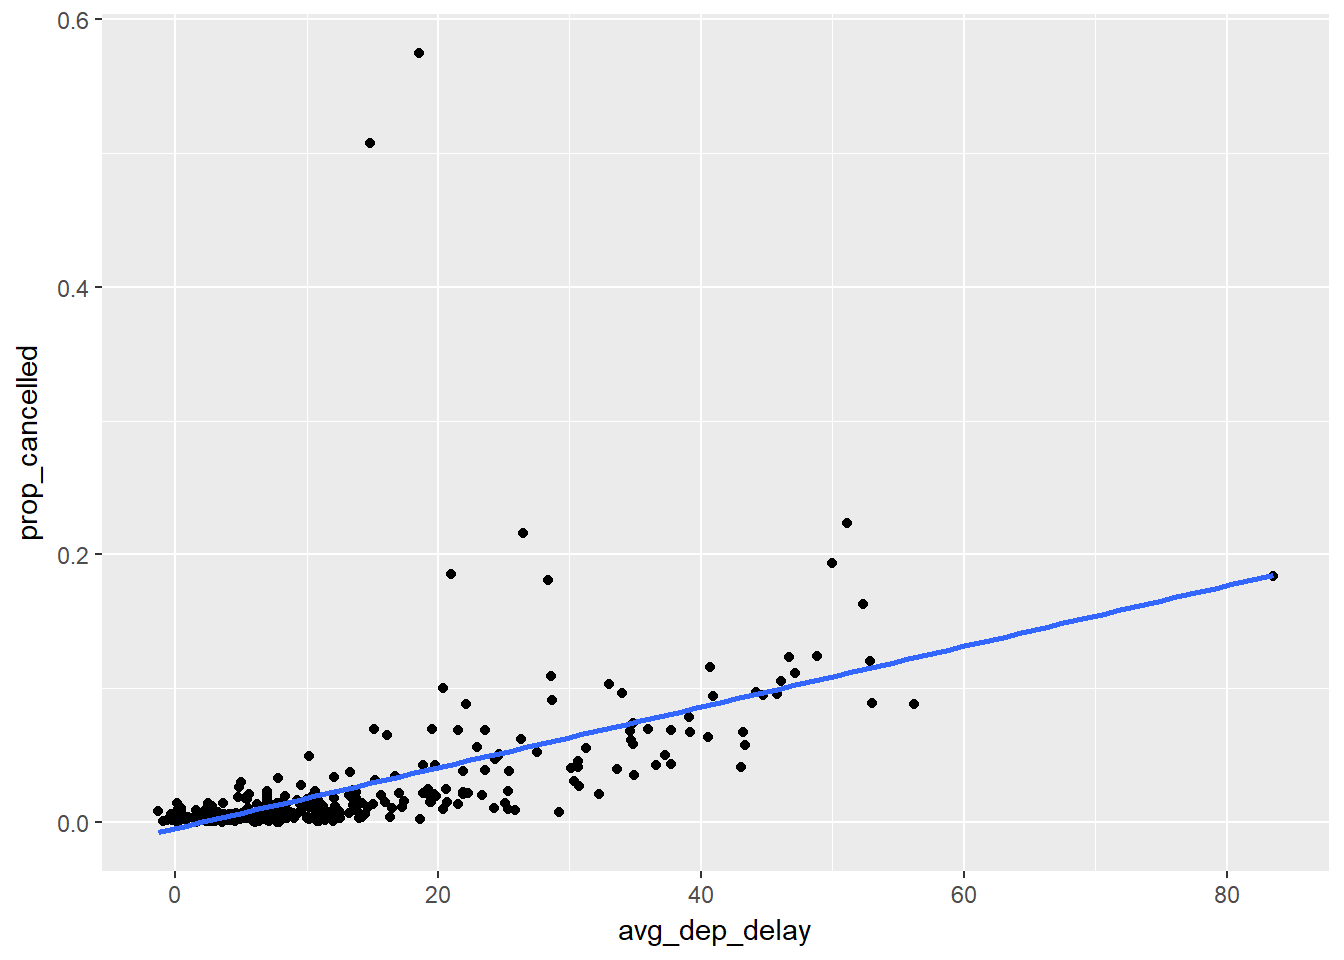
\includegraphics{R4DS_bookdown_files/figure-latex/unnamed-chunk-86-1.pdf}

\emph{5 - Which carrier has the worst delays? Challenge: can you
disentangle the effects of bad airports vs.~bad carriers? Why/why not?
(Hint: think about
\texttt{flights\ \%\textgreater{}\%\ group\_by(carrier,\ dest)\ \%\textgreater{}\%\ summarise(n())})}

First we need to decide how we quantify and compare delays between
carriers. For this question we'll just simply calculate the average
minutes in arrival and departure delays.

\begin{Shaded}
\begin{Highlighting}[]
\NormalTok{worst <-}\StringTok{ }\NormalTok{flights }\OperatorTok\StringTok{ }\KeywordTok{group_by}\NormalTok{(carrier) }\OperatorTok\StringTok{ }
\StringTok{  }\KeywordTok{summarize}\NormalTok{(}\DataTypeTok{avg_arr_delay =} \KeywordTok{mean}\NormalTok{(arr_delay, }\DataTypeTok{na.rm =} \OtherTok{TRUE}\NormalTok{),}
            \DataTypeTok{avg_dep_delay =} \KeywordTok{mean}\NormalTok{(dep_delay, }\DataTypeTok{na.rm =} \OtherTok{TRUE}\NormalTok{))}
\end{Highlighting}
\end{Shaded}

Arrange by average arrival delay in minutes:

\begin{Shaded}
\begin{Highlighting}[]
\KeywordTok{arrange}\NormalTok{(worst, }\KeywordTok{desc}\NormalTok{(avg_arr_delay))}
\end{Highlighting}
\end{Shaded}

\begin{verbatim}
## # A tibble: 16 x 3
##    carrier avg_arr_delay avg_dep_delay
##    <chr>           <dbl>         <dbl>
##  1 F9             21.9           20.2 
##  2 FL             20.1           18.7 
##  3 EV             15.8           20.0 
##  4 YV             15.6           19.0 
##  5 OO             11.9           12.6 
##  6 MQ             10.8           10.6 
##  7 WN              9.65          17.7 
##  8 B6              9.46          13.0 
##  9 9E              7.38          16.7 
## 10 UA              3.56          12.1 
## 11 US              2.13           3.78
## 12 VX              1.76          12.9 
## 13 DL              1.64           9.26
## 14 AA              0.364          8.59
## 15 HA            - 6.92           4.90
## 16 AS            - 9.93           5.80
\end{verbatim}

Arrange by average departure delay in minutes:

\begin{Shaded}
\begin{Highlighting}[]
\KeywordTok{arrange}\NormalTok{(worst, }\KeywordTok{desc}\NormalTok{(avg_dep_delay))}
\end{Highlighting}
\end{Shaded}

\begin{verbatim}
## # A tibble: 16 x 3
##    carrier avg_arr_delay avg_dep_delay
##    <chr>           <dbl>         <dbl>
##  1 F9             21.9           20.2 
##  2 EV             15.8           20.0 
##  3 YV             15.6           19.0 
##  4 FL             20.1           18.7 
##  5 WN              9.65          17.7 
##  6 9E              7.38          16.7 
##  7 B6              9.46          13.0 
##  8 VX              1.76          12.9 
##  9 OO             11.9           12.6 
## 10 UA              3.56          12.1 
## 11 MQ             10.8           10.6 
## 12 DL              1.64           9.26
## 13 AA              0.364          8.59
## 14 AS            - 9.93           5.80
## 15 HA            - 6.92           4.90
## 16 US              2.13           3.78
\end{verbatim}

Similarly we can look at which airport has the worst departure delay:

\begin{Shaded}
\begin{Highlighting}[]
\NormalTok{flights }\OperatorTok\StringTok{ }\KeywordTok{group_by}\NormalTok{(origin) }\OperatorTok
\StringTok{  }\KeywordTok{summarize}\NormalTok{(}\DataTypeTok{avg_dep_delay =} \KeywordTok{mean}\NormalTok{(dep_delay, }\DataTypeTok{na.rm =} \OtherTok{TRUE}\NormalTok{)) }
\end{Highlighting}
\end{Shaded}

\begin{verbatim}
## # A tibble: 3 x 2
##   origin avg_dep_delay
##   <chr>          <dbl>
## 1 EWR             15.1
## 2 JFK             12.1
## 3 LGA             10.3
\end{verbatim}

and the worst arrival delay:

\begin{Shaded}
\begin{Highlighting}[]
\NormalTok{flights }\OperatorTok\StringTok{ }\KeywordTok{group_by}\NormalTok{(origin) }\OperatorTok
\StringTok{  }\KeywordTok{summarize}\NormalTok{(}\DataTypeTok{avg_arr_delay =} \KeywordTok{mean}\NormalTok{(arr_delay, }\DataTypeTok{na.rm =} \OtherTok{TRUE}\NormalTok{)) }
\end{Highlighting}
\end{Shaded}

\begin{verbatim}
## # A tibble: 3 x 2
##   origin avg_arr_delay
##   <chr>          <dbl>
## 1 EWR             9.11
## 2 JFK             5.55
## 3 LGA             5.78
\end{verbatim}

We can attempt to disentangle the effects of departure delay for carrier
\texttt{9E}:

\begin{Shaded}
\begin{Highlighting}[]
\NormalTok{flights }\OperatorTok\StringTok{ }\KeywordTok{group_by}\NormalTok{(carrier, origin) }\OperatorTok
\StringTok{  }\KeywordTok{summarize}\NormalTok{(}\DataTypeTok{avg_dep_delay =} \KeywordTok{mean}\NormalTok{(dep_delay, }\DataTypeTok{na.rm =} \OtherTok{TRUE}\NormalTok{)) }\OperatorTok
\StringTok{  }\KeywordTok{filter}\NormalTok{(carrier }\OperatorTok{==}\StringTok{ '9E'}\NormalTok{)}
\end{Highlighting}
\end{Shaded}

\begin{verbatim}
## # A tibble: 3 x 3
## # Groups:   carrier [1]
##   carrier origin avg_dep_delay
##   <chr>   <chr>          <dbl>
## 1 9E      EWR             5.95
## 2 9E      JFK            19.0 
## 3 9E      LGA             8.89
\end{verbatim}

The overall average departure delay is 16.73 minutes from the previous
table. However, we can conclude that at least for carrier \texttt{9E},
on average, the flights were delayed most at JFK.

\emph{6 - What does the sort argument to count() do. When might you use
it?}

The \texttt{sort} argument if set to \texttt{TRUE}, will sort the output
in descending order. For example, without \texttt{sort\ =\ TRUE}:

\begin{Shaded}
\begin{Highlighting}[]
\NormalTok{flights }\OperatorTok\StringTok{ }
\StringTok{  }\KeywordTok{filter}\NormalTok{(}\OperatorTok{!}\KeywordTok{is.na}\NormalTok{(dep_delay), }\OperatorTok{!}\KeywordTok{is.na}\NormalTok{(arr_delay)) }\OperatorTok
\StringTok{  }\KeywordTok{count}\NormalTok{(dest)}
\end{Highlighting}
\end{Shaded}

\begin{verbatim}
## # A tibble: 104 x 2
##    dest      n
##    <chr> <int>
##  1 ABQ     254
##  2 ACK     264
##  3 ALB     418
##  4 ANC       8
##  5 ATL   16837
##  6 AUS    2411
##  7 AVL     261
##  8 BDL     412
##  9 BGR     358
## 10 BHM     269
## # ... with 94 more rows
\end{verbatim}

With \texttt{sort\ =\ TRUE}:

\begin{Shaded}
\begin{Highlighting}[]
\NormalTok{flights }\OperatorTok\StringTok{ }
\StringTok{  }\KeywordTok{filter}\NormalTok{(}\OperatorTok{!}\KeywordTok{is.na}\NormalTok{(dep_delay), }\OperatorTok{!}\KeywordTok{is.na}\NormalTok{(arr_delay)) }\OperatorTok
\StringTok{  }\KeywordTok{count}\NormalTok{(dest, }\DataTypeTok{sort =} \OtherTok{TRUE}\NormalTok{)}
\end{Highlighting}
\end{Shaded}

\begin{verbatim}
## # A tibble: 104 x 2
##    dest      n
##    <chr> <int>
##  1 ATL   16837
##  2 ORD   16566
##  3 LAX   16026
##  4 BOS   15022
##  5 MCO   13967
##  6 CLT   13674
##  7 SFO   13173
##  8 FLL   11897
##  9 MIA   11593
## 10 DCA    9111
## # ... with 94 more rows
\end{verbatim}

\subsection{Grouped mutates (and
filters)}\label{grouped-mutates-and-filters}

\subsubsection{Exercises}\label{exercises-12}

\emph{1 - Refer back to the lists of useful mutate and filtering
functions. Describe how each operation changes when you combine it with
grouping.}

Before grouping, functions like \texttt{mean()}, \texttt{median()},
\texttt{min()}, or \texttt{max()} will operation over the whole dataset.
For example, applying \texttt{mean()} on a variable before grouping will
get the average of the variable over the entire dataset.

After grouping, these functions will operate within each group.

\emph{2 - Which plane (\texttt{tailnum}) has the worst on-time record?}

Filter out the on-time departure records and calculate the average
departure delay in minutes.

\begin{Shaded}
\begin{Highlighting}[]
\NormalTok{flights }\OperatorTok\StringTok{ }\KeywordTok{group_by}\NormalTok{(tailnum) }\OperatorTok
\StringTok{  }\KeywordTok{filter}\NormalTok{(dep_delay }\OperatorTok{>}\StringTok{ }\DecValTok{0}\NormalTok{) }\OperatorTok
\StringTok{  }\KeywordTok{summarize}\NormalTok{(}\DataTypeTok{avg_delay =} \KeywordTok{mean}\NormalTok{(dep_delay)) }\OperatorTok
\StringTok{  }\KeywordTok{arrange}\NormalTok{(}\KeywordTok{desc}\NormalTok{(avg_delay))}
\end{Highlighting}
\end{Shaded}

\begin{verbatim}
## # A tibble: 3,885 x 2
##    tailnum avg_delay
##    <chr>       <dbl>
##  1 N844MH        297
##  2 N452UW        291
##  3 N922EV        274
##  4 N587NW        272
##  5 N911DA        268
##  6 N665MQ        268
##  7 N673MQ        257
##  8 N851NW        233
##  9 N654UA        227
## 10 N550NW        212
## # ... with 3,875 more rows
\end{verbatim}

\emph{3 - What time of day should you fly if you want to avoid delays as
much as possible?}

Similar to above question, we filter out the on-time departures and
calculate the average departure delay in minuts for each hour.

\begin{Shaded}
\begin{Highlighting}[]
\NormalTok{flights }\OperatorTok\StringTok{ }\KeywordTok{filter}\NormalTok{ (dep_delay }\OperatorTok{>}\StringTok{ }\DecValTok{0}\NormalTok{) }\OperatorTok\StringTok{ }
\StringTok{  }\KeywordTok{group_by}\NormalTok{(hour) }\OperatorTok
\StringTok{  }\KeywordTok{summarize}\NormalTok{(}\DataTypeTok{avg_delay =} \KeywordTok{mean}\NormalTok{(dep_delay)) }\OperatorTok
\StringTok{  }\KeywordTok{arrange}\NormalTok{(avg_delay)}
\end{Highlighting}
\end{Shaded}

\begin{verbatim}
## # A tibble: 19 x 2
##     hour avg_delay
##    <dbl>     <dbl>
##  1  5.00      15.3
##  2  7.00      24.1
##  3  6.00      24.2
##  4  9.00      29.7
##  5  8.00      29.9
##  6 12.0       32.3
##  7 11.0       32.5
##  8 10.0       32.6
##  9 13.0       33.5
## 10 14.0       37.1
## 11 23.0       38.0
## 12 15.0       38.8
## 13 16.0       43.4
## 14 17.0       45.3
## 15 18.0       46.5
## 16 22.0       46.5
## 17 20.0       49.6
## 18 21.0       50.3
## 19 19.0       51.1
\end{verbatim}

\emph{4 - For each destination, compute the total minutes of delay. For
each flight, compute the proportion of the total delay for its
destination.}

We select only \texttt{dest} and \texttt{arr\_delay} variables. We also
filter out on-time flights or flights that were cancelled.

\begin{Shaded}
\begin{Highlighting}[]
\NormalTok{flights }\OperatorTok\StringTok{ }\KeywordTok{select}\NormalTok{(dest, arr_delay) }\OperatorTok\StringTok{ }\KeywordTok{group_by}\NormalTok{(dest) }\OperatorTok
\StringTok{  }\KeywordTok{filter}\NormalTok{(arr_delay }\OperatorTok{>}\StringTok{ }\DecValTok{0}\NormalTok{) }\OperatorTok
\StringTok{  }\KeywordTok{mutate}\NormalTok{(}\DataTypeTok{total_delay =} \KeywordTok{sum}\NormalTok{(arr_delay, }\DataTypeTok{na.rm =} \OtherTok{TRUE}\NormalTok{),}
         \DataTypeTok{prop_delay =}\NormalTok{ arr_delay }\OperatorTok{/}\StringTok{ }\NormalTok{total_delay)}
\end{Highlighting}
\end{Shaded}

\begin{verbatim}
## # A tibble: 133,004 x 4
## # Groups:   dest [103]
##    dest  arr_delay total_delay prop_delay
##    <chr>     <dbl>       <dbl>      <dbl>
##  1 IAH       11.0        99391  0.000111 
##  2 IAH       20.0        99391  0.000201 
##  3 MIA       33.0       140424  0.000235 
##  4 ORD       12.0       283046  0.0000424
##  5 FLL       19.0       202605  0.0000938
##  6 ORD        8.00      283046  0.0000283
##  7 LAX        7.00      203226  0.0000344
##  8 DFW       31.0       110009  0.000282 
##  9 ATL       12.0       300299  0.0000400
## 10 DTW       16.0       138258  0.000116 
## # ... with 132,994 more rows
\end{verbatim}

\emph{5 - Delays are typically temporally correlated: even once the
problem that caused the initial delay has been resolved, later flights
are delayed to allow earlier flights to leave. Using \texttt{lag()}
explore how the delay of a flight is related to the delay of the
immediately preceding flight.}

Let's focus on flights departing from \texttt{JFK} and assume we can
ignore the effect of cancelled flights:

\begin{Shaded}
\begin{Highlighting}[]
\NormalTok{flights }\OperatorTok\StringTok{ }\KeywordTok{filter}\NormalTok{(origin }\OperatorTok{==}\StringTok{ 'JFK'}\NormalTok{) }\OperatorTok\StringTok{ }\KeywordTok{filter}\NormalTok{(}\OperatorTok{!}\KeywordTok{is.na}\NormalTok{(dep_delay)) }\OperatorTok
\StringTok{  }\KeywordTok{mutate}\NormalTok{(}\DataTypeTok{pre_dep_delay =} \KeywordTok{lag}\NormalTok{(dep_delay, }\DataTypeTok{default =} \DecValTok{0}\NormalTok{)) }\OperatorTok
\StringTok{  }\KeywordTok{ggplot}\NormalTok{(}\DataTypeTok{mapping =} \KeywordTok{aes}\NormalTok{(}\DataTypeTok{x =}\NormalTok{ dep_delay, }\DataTypeTok{y=}\NormalTok{ pre_dep_delay)) }\OperatorTok{+}
\StringTok{  }\KeywordTok{geom_point}\NormalTok{(}\DataTypeTok{alpha =}\NormalTok{ .}\DecValTok{5}\NormalTok{)}
\end{Highlighting}
\end{Shaded}

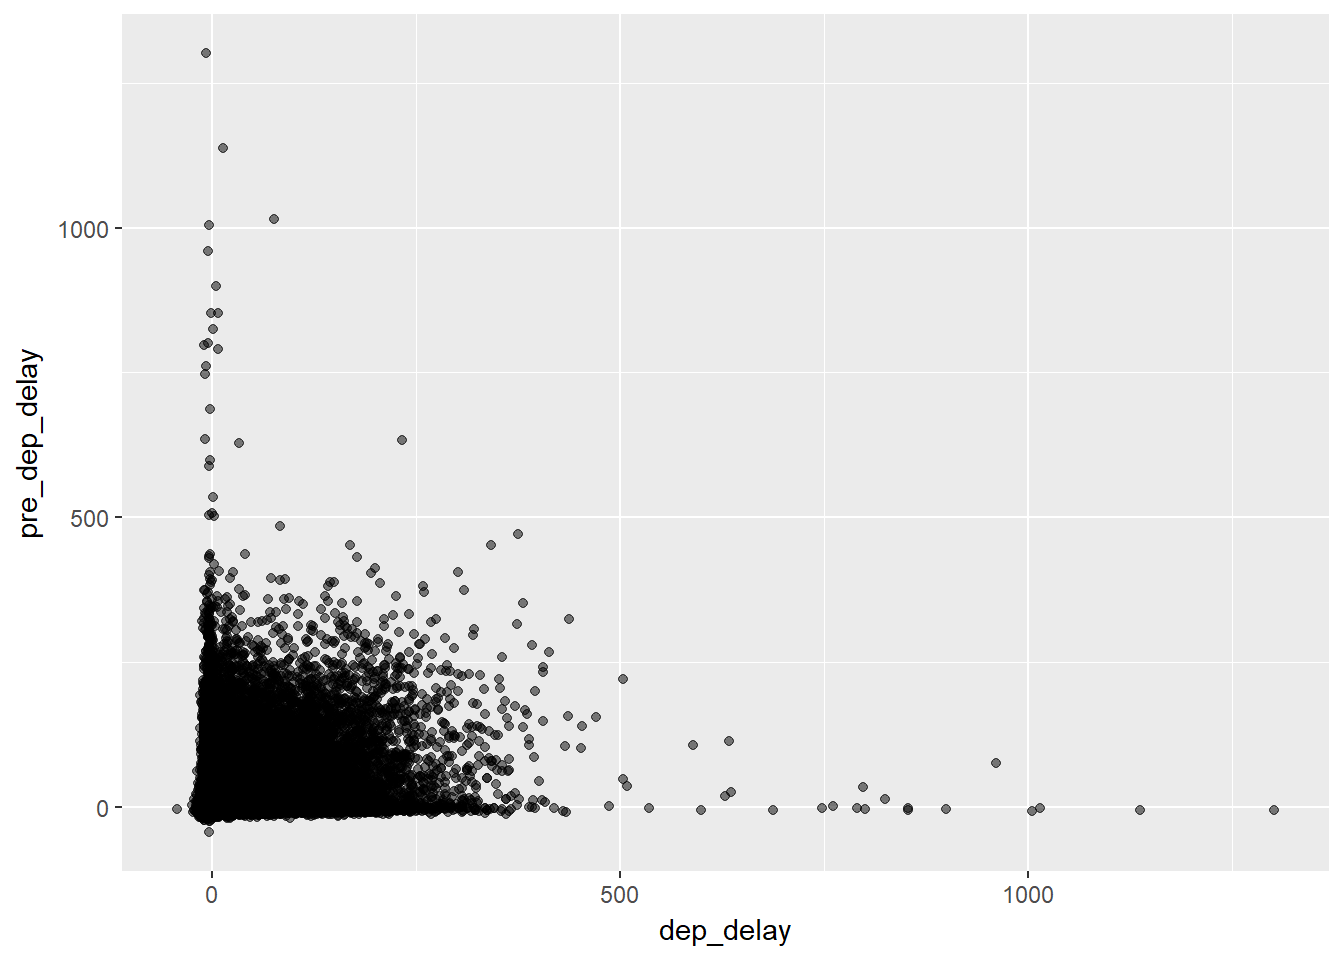
\includegraphics{R4DS_bookdown_files/figure-latex/unnamed-chunk-98-1.pdf}

The mass of data on the bottom left shows that the departure delay and
the previous depart delay are related. The correlation is:

\begin{Shaded}
\begin{Highlighting}[]
\NormalTok{flights <-}\StringTok{ }\NormalTok{flights }\OperatorTok\StringTok{ }\KeywordTok{filter}\NormalTok{(origin }\OperatorTok{==}\StringTok{ 'JFK'}\NormalTok{) }\OperatorTok\StringTok{ }\KeywordTok{filter}\NormalTok{(}\OperatorTok{!}\KeywordTok{is.na}\NormalTok{(dep_delay)) }\OperatorTok
\StringTok{  }\KeywordTok{mutate}\NormalTok{(}\DataTypeTok{pre_dep_delay =} \KeywordTok{lag}\NormalTok{(dep_delay, }\DataTypeTok{default =} \DecValTok{0}\NormalTok{))}

\KeywordTok{cor}\NormalTok{(flights}\OperatorTok{$}\NormalTok{dep_delay, flights}\OperatorTok{$}\NormalTok{pre_dep_delay)}
\end{Highlighting}
\end{Shaded}

\begin{verbatim}
## [1] 0.2928064
\end{verbatim}

\emph{6 - Look at each destination. Can you find flights that are
suspiciously fast? (i.e.~flights that represent a potential data entry
error). Compute the air time a flight relative to the shortest flight to
that destination. Which flights were most delayed in the air?}

To find flights that are suspiciously fast, in other words, outliers
that are far below than the average \texttt{air\_time}, we can compute
z-score, or the number of standard deviations below/above the mean
\texttt{air\_time}.

\begin{Shaded}
\begin{Highlighting}[]
\NormalTok{flights }\OperatorTok\StringTok{ }\KeywordTok{filter}\NormalTok{(}\OperatorTok{!}\KeywordTok{is.na}\NormalTok{(air_time)) }\OperatorTok\StringTok{ }\KeywordTok{group_by}\NormalTok{(dest) }\OperatorTok
\StringTok{  }\KeywordTok{mutate}\NormalTok{(}\DataTypeTok{air_time_mean =} \KeywordTok{mean}\NormalTok{(air_time),}
         \DataTypeTok{air_time_sd =} \KeywordTok{sd}\NormalTok{(air_time),}
         \DataTypeTok{z =}\NormalTok{ (air_time }\OperatorTok{-}\StringTok{ }\NormalTok{air_time_mean) }\OperatorTok{/}\StringTok{ }\NormalTok{air_time_sd) }\OperatorTok
\StringTok{  }\KeywordTok{select}\NormalTok{(z, air_time_mean, dest, }\KeywordTok{everything}\NormalTok{()) }\OperatorTok
\StringTok{  }\KeywordTok{arrange}\NormalTok{(z)}
\end{Highlighting}
\end{Shaded}

\begin{verbatim}
## # A tibble: 109,079 x 27
## # Groups:   dest [70]
##        z air_time_mean dest   year month   day dep_time sched_dep_time
##    <dbl>         <dbl> <chr> <int> <int> <int>    <int>          <int>
##  1 -4.10          57.1 BUF    2013    11    10     2307           2250
##  2 -3.80          51.9 ROC    2013     3    25     2340           2250
##  3 -3.55         329   SEA    2013     7     3     1533           1459
##  4 -3.51          52.6 ORF    2013    11     3     1720           1645
##  5 -3.40          66.5 PIT    2013     7    17     1504           1505
##  6 -3.03          66.5 PIT    2013     5     8     1947           1859
##  7 -3.03         329   SEA    2013     5     6     1728           1730
##  8 -2.99         331   PDX    2013     5     6     1753           1755
##  9 -2.98         329   LAX    2013     9     6     2042           2025
## 10 -2.97         329   SEA    2013     5     6     1553           1557
## # ... with 109,069 more rows, and 19 more variables: dep_delay <dbl>,
## #   arr_time <int>, sched_arr_time <int>, arr_delay <dbl>, carrier <chr>,
## #   flight <int>, tailnum <chr>, origin <chr>, air_time <dbl>,
## #   distance <dbl>, hour <dbl>, minute <dbl>, time_hour <dttm>,
## #   dep_time_mins <dbl>, sched_dep_time_mins <dbl>, arr_time_mins <dbl>,
## #   flight_time <dbl>, pre_dep_delay <dbl>, air_time_sd <dbl>
\end{verbatim}

I would say that \texttt{air\_time} that are 2 standard deviations below
the are unusually fast.

Similarly we can look at which flights are most delayed in the air.

\begin{Shaded}
\begin{Highlighting}[]
\NormalTok{flights }\OperatorTok\StringTok{ }\KeywordTok{filter}\NormalTok{(}\OperatorTok{!}\KeywordTok{is.na}\NormalTok{(air_time)) }\OperatorTok\StringTok{ }\KeywordTok{group_by}\NormalTok{(dest) }\OperatorTok
\StringTok{  }\KeywordTok{mutate}\NormalTok{(}\DataTypeTok{air_time_mean =} \KeywordTok{mean}\NormalTok{(air_time),}
         \DataTypeTok{air_time_sd =} \KeywordTok{sd}\NormalTok{(air_time),}
         \DataTypeTok{z =}\NormalTok{ (air_time }\OperatorTok{-}\StringTok{ }\NormalTok{air_time_mean) }\OperatorTok{/}\StringTok{ }\NormalTok{air_time_sd) }\OperatorTok
\StringTok{  }\KeywordTok{select}\NormalTok{(z, air_time_mean, dest, }\KeywordTok{everything}\NormalTok{()) }\OperatorTok
\StringTok{  }\KeywordTok{arrange}\NormalTok{(}\KeywordTok{desc}\NormalTok{(z))}
\end{Highlighting}
\end{Shaded}

\begin{verbatim}
## # A tibble: 109,079 x 27
## # Groups:   dest [70]
##        z air_time_mean dest   year month   day dep_time sched_dep_time
##    <dbl>         <dbl> <chr> <int> <int> <int>    <int>          <int>
##  1 13.9           44.5 SYR    2013     9     1     2237           1711
##  2 12.2           42.1 ACK    2013     6    29      755            800
##  3 11.8           38.5 BOS    2013     7    23     1617           1605
##  4 10.8           38.5 BOS    2013     7    23     1200           1200
##  5 10.4           71.9 RDU    2013     9     1     1719           1712
##  6 10.3           57.1 BUF    2013    12    16      923            925
##  7  9.91          87.6 DTW    2013     7    27     1654           1620
##  8  9.74          38.5 BOS    2013     2    17      841            840
##  9  9.74          38.5 BOS    2013     7    23     1242           1245
## 10  9.69          51.9 ROC    2013     7    10     2350           2030
## # ... with 109,069 more rows, and 19 more variables: dep_delay <dbl>,
## #   arr_time <int>, sched_arr_time <int>, arr_delay <dbl>, carrier <chr>,
## #   flight <int>, tailnum <chr>, origin <chr>, air_time <dbl>,
## #   distance <dbl>, hour <dbl>, minute <dbl>, time_hour <dttm>,
## #   dep_time_mins <dbl>, sched_dep_time_mins <dbl>, arr_time_mins <dbl>,
## #   flight_time <dbl>, pre_dep_delay <dbl>, air_time_sd <dbl>
\end{verbatim}

10 standard deviations above the mean!

\emph{7 - Find all destinations that are flown by at least two carriers.
Use that information to rank the carriers.}

Destinations that are flown by the most number of carriers:

\begin{Shaded}
\begin{Highlighting}[]
\NormalTok{flights }\OperatorTok\StringTok{ }\KeywordTok{group_by}\NormalTok{(dest) }\OperatorTok
\StringTok{  }\KeywordTok{summarise}\NormalTok{(}\DataTypeTok{num_carrier =} \KeywordTok{length}\NormalTok{(}\KeywordTok{unique}\NormalTok{(carrier))) }\OperatorTok
\StringTok{  }\KeywordTok{filter}\NormalTok{(num_carrier }\OperatorTok{>=}\StringTok{ }\DecValTok{2}\NormalTok{) }\OperatorTok
\StringTok{  }\KeywordTok{arrange}\NormalTok{(}\KeywordTok{desc}\NormalTok{(num_carrier))}
\end{Highlighting}
\end{Shaded}

\begin{verbatim}
## # A tibble: 45 x 2
##    dest  num_carrier
##    <chr>       <int>
##  1 LAX             5
##  2 SFO             5
##  3 TPA             5
##  4 AUS             4
##  5 BOS             4
##  6 LAS             4
##  7 PIT             4
##  8 ATL             3
##  9 BNA             3
## 10 CLT             3
## # ... with 35 more rows
\end{verbatim}

Similiar, we can rank the carriers by counting how many destinations
they fly to:

\begin{Shaded}
\begin{Highlighting}[]
\NormalTok{flights }\OperatorTok\StringTok{ }\KeywordTok{group_by}\NormalTok{(carrier) }\OperatorTok
\StringTok{  }\KeywordTok{summarise}\NormalTok{(}\DataTypeTok{num_dest =} \KeywordTok{length}\NormalTok{(}\KeywordTok{unique}\NormalTok{(dest))) }\OperatorTok
\StringTok{  }\KeywordTok{filter}\NormalTok{(num_dest }\OperatorTok{>=}\StringTok{ }\DecValTok{2}\NormalTok{) }\OperatorTok
\StringTok{  }\KeywordTok{arrange}\NormalTok{(}\KeywordTok{desc}\NormalTok{(num_dest))}
\end{Highlighting}
\end{Shaded}

\begin{verbatim}
## # A tibble: 9 x 2
##   carrier num_dest
##   <chr>      <int>
## 1 B6            42
## 2 9E            34
## 3 DL            29
## 4 AA            17
## 5 MQ            11
## 6 VX             5
## 7 EV             3
## 8 US             3
## 9 UA             2
\end{verbatim}

\emph{8 - For each plane, count the number of flights before the first
delay of greater than 1 hour.}

Not sure if this is the most elegant solution. Let's assume we can
ignore the cancelled flights. We group by \texttt{tailnum}, and use
\texttt{cummax()} to find the cummulative maxium departure delay. Count
the total number of observations with cummulative max less than 60.

\begin{Shaded}
\begin{Highlighting}[]
\NormalTok{flights }\OperatorTok\StringTok{ }\KeywordTok{filter}\NormalTok{(}\OperatorTok{!}\KeywordTok{is.na}\NormalTok{(dep_delay)) }\OperatorTok\StringTok{ }\KeywordTok{group_by}\NormalTok{(tailnum) }\OperatorTok
\StringTok{  }\KeywordTok{mutate}\NormalTok{(}\DataTypeTok{max_delay =} \KeywordTok{cummax}\NormalTok{(dep_delay),}
         \DataTypeTok{less_one_hour =}\NormalTok{ max_delay }\OperatorTok{<}\StringTok{ }\DecValTok{60}\NormalTok{) }\OperatorTok
\StringTok{  }\KeywordTok{summarize}\NormalTok{(}\DataTypeTok{count =} \KeywordTok{sum}\NormalTok{(less_one_hour)) }\OperatorTok
\StringTok{  }\KeywordTok{arrange}\NormalTok{(}\KeywordTok{desc}\NormalTok{(count))}
\end{Highlighting}
\end{Shaded}

\begin{verbatim}
## # A tibble: 1,957 x 2
##    tailnum count
##    <chr>   <int>
##  1 N705TW    159
##  2 N706TW    149
##  3 N713TW    128
##  4 N721TW    120
##  5 N5FAAA    117
##  6 N3769L    104
##  7 N804JB    104
##  8 N3748Y    103
##  9 N645JB     94
## 10 N3742C     91
## # ... with 1,947 more rows
\end{verbatim}

\section{Workflow: scripts}\label{workflow-scripts}

No exercises.

\section{Exploratory Data Analysis}\label{exploratory-data-analysis}

\subsection{Introduction}\label{introduction-4}

No exercises.

\subsection{Questions}\label{questions}

No exercises.

\subsection{Variation}\label{variation}

\subsubsection{Exercises}\label{exercises-13}

\emph{1 - Explore the distribution of each of the \texttt{x},
\texttt{y}, and \texttt{z} variables in diamonds. What do you learn?
Think about a diamond and how you might decide which dimension is the
length, width, and depth.}

\begin{Shaded}
\begin{Highlighting}[]
\KeywordTok{library}\NormalTok{(tidyverse)}
\end{Highlighting}
\end{Shaded}

The description of \texttt{x}, \texttt{y}, and \texttt{z} variables are
given in \texttt{?diamonds}. We can still explore the distributions of
these three dimensions. One option is to use \texttt{geom\_histogram()}.
Another option is to use \texttt{geom\_density()}, which is a smoothed
version of the histogram. Here we will use \texttt{geom\_density()}
along with \texttt{geom\_rug()}, which shows a 1-dimensional
distribution at the bottom.

\begin{Shaded}
\begin{Highlighting}[]
\KeywordTok{ggplot}\NormalTok{(}\DataTypeTok{data =}\NormalTok{ diamonds, }\DataTypeTok{mapping =} \KeywordTok{aes}\NormalTok{(}\DataTypeTok{x =}\NormalTok{ x)) }\OperatorTok{+}
\StringTok{  }\KeywordTok{geom_density}\NormalTok{() }\OperatorTok{+}\StringTok{ }
\StringTok{  }\KeywordTok{geom_rug}\NormalTok{() }\OperatorTok{+}
\StringTok{  }\KeywordTok{labs}\NormalTok{(}\DataTypeTok{title =} \StringTok{'Distribution of x(length)'}\NormalTok{)}
\end{Highlighting}
\end{Shaded}

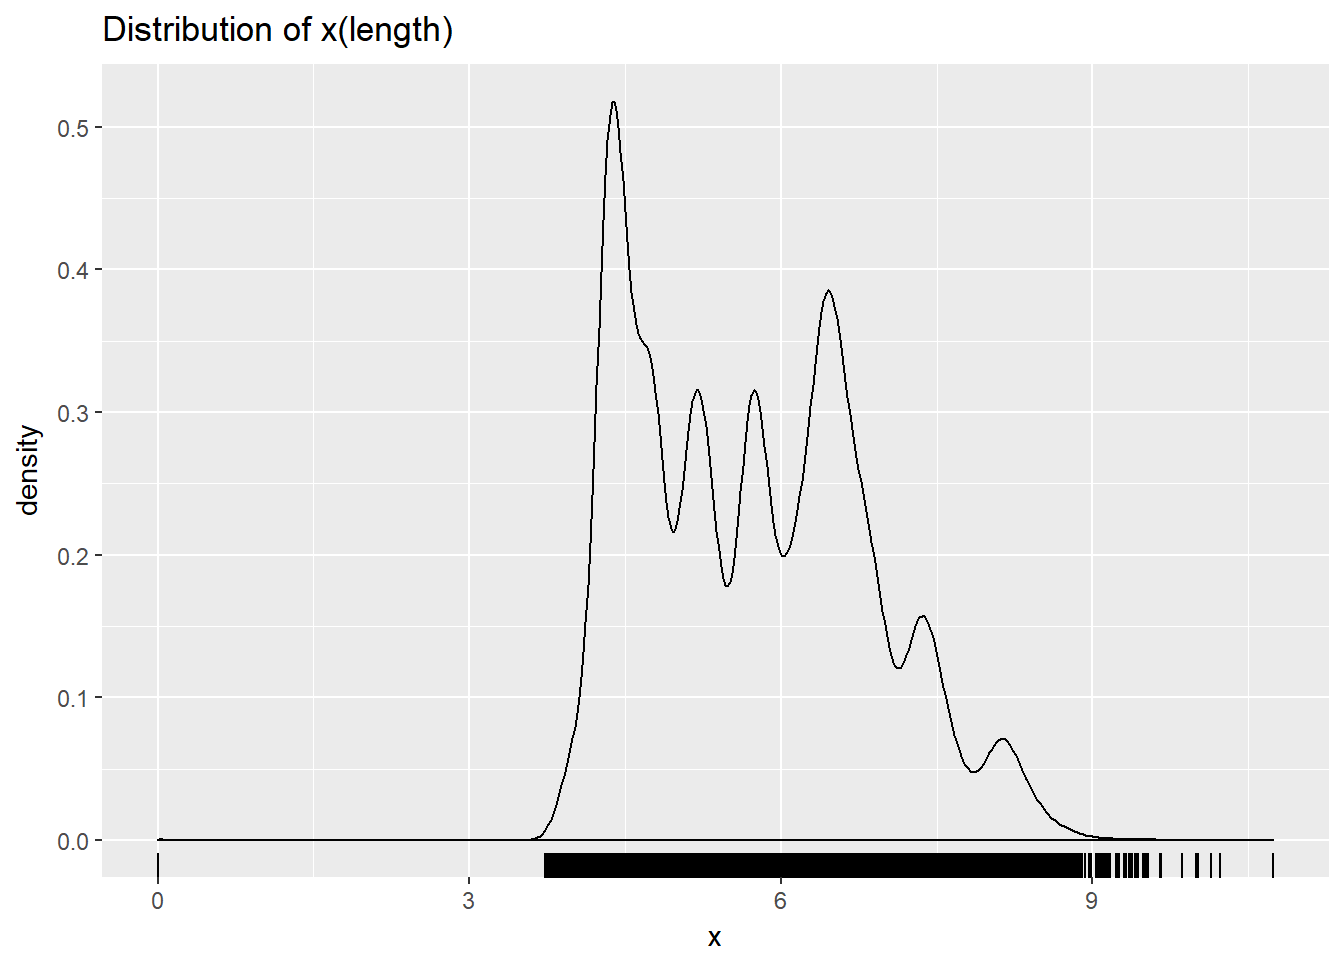
\includegraphics{R4DS_bookdown_files/figure-latex/unnamed-chunk-106-1.pdf}

\begin{Shaded}
\begin{Highlighting}[]
\KeywordTok{ggplot}\NormalTok{(}\DataTypeTok{data =}\NormalTok{ diamonds, }\DataTypeTok{mapping =} \KeywordTok{aes}\NormalTok{(}\DataTypeTok{x =}\NormalTok{ y)) }\OperatorTok{+}
\StringTok{  }\KeywordTok{geom_density}\NormalTok{() }\OperatorTok{+}
\StringTok{  }\KeywordTok{geom_rug}\NormalTok{() }\OperatorTok{+}
\StringTok{  }\KeywordTok{labs}\NormalTok{(}\DataTypeTok{title =} \StringTok{'Distribution of y(width)'}\NormalTok{)}
\end{Highlighting}
\end{Shaded}

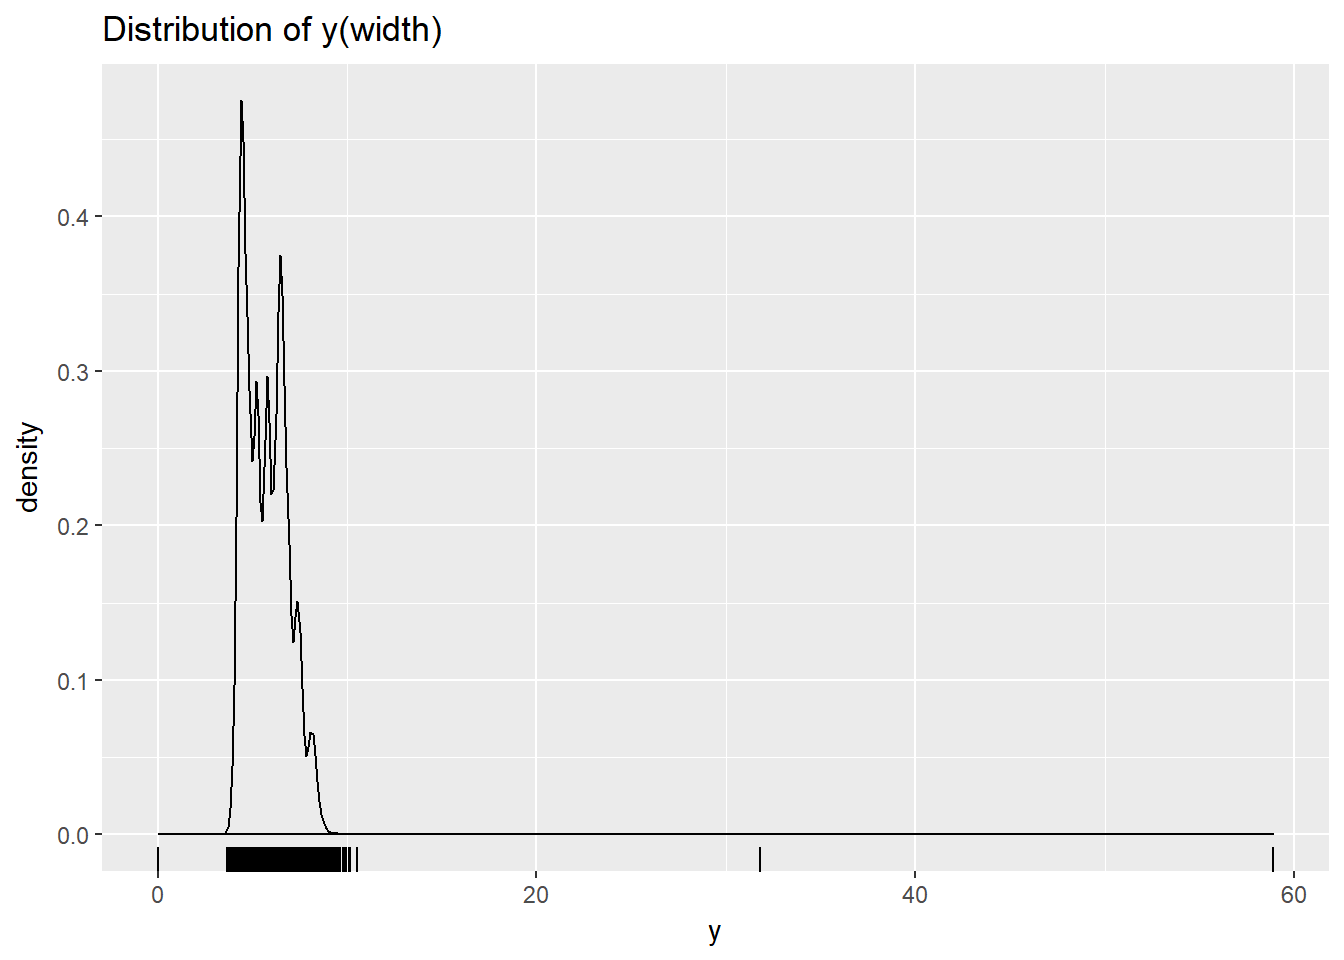
\includegraphics{R4DS_bookdown_files/figure-latex/unnamed-chunk-107-1.pdf}

\begin{Shaded}
\begin{Highlighting}[]
\KeywordTok{ggplot}\NormalTok{(}\DataTypeTok{data =}\NormalTok{ diamonds, }\DataTypeTok{mapping =} \KeywordTok{aes}\NormalTok{(}\DataTypeTok{x =}\NormalTok{ z)) }\OperatorTok{+}
\StringTok{  }\KeywordTok{geom_density}\NormalTok{() }\OperatorTok{+}\StringTok{ }
\StringTok{  }\KeywordTok{geom_rug}\NormalTok{() }\OperatorTok{+}
\StringTok{  }\KeywordTok{labs}\NormalTok{(}\DataTypeTok{title =} \StringTok{'Distribution of z(depth)'}\NormalTok{)}
\end{Highlighting}
\end{Shaded}

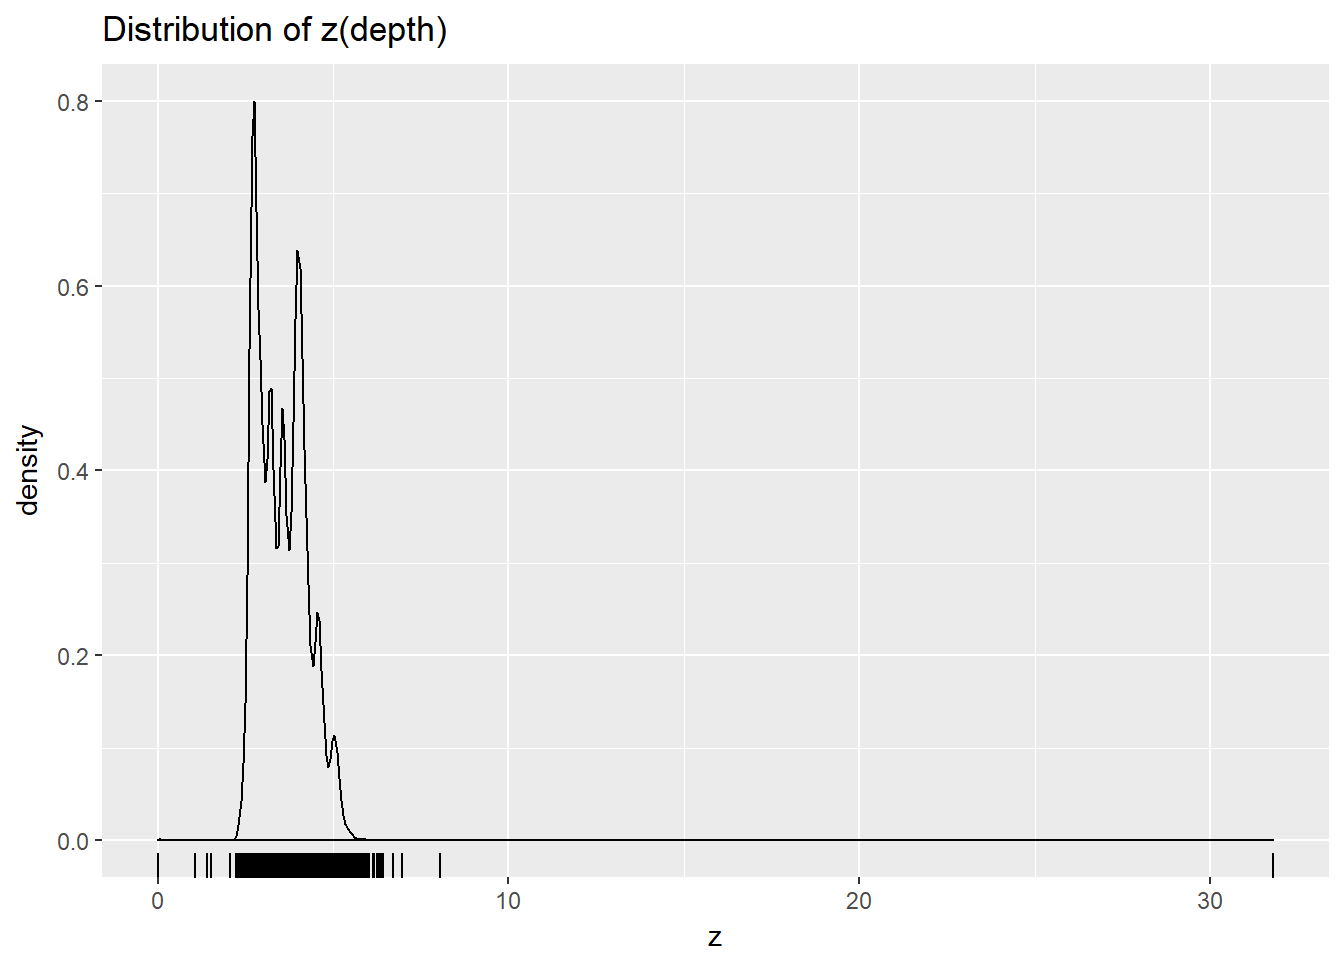
\includegraphics{R4DS_bookdown_files/figure-latex/unnamed-chunk-108-1.pdf}

We see that in general, there are more smaller diamonds than bigger
ones. Also in \texttt{y} and \texttt{z} dimensions, there are outliers.
They could be errros or real diamonds that are exceptionally large.

\emph{2 - Explore the distribution of \texttt{price}. Do you discover
anything unusual or surprising? (Hint: Carefully think about the
\texttt{binwidth} and make sure you try a wide range of values.)}

Setting the \texttt{binwidth} to 20, we can see that the price
distribution is right-skewed and has many `spikes'. Most of the diamonds
are under 1,000, and interestingly and unusally there are no dimaonds in
the price range of around 1,500. There is also an increase in the number
of diamonds in the price range of raound 4,500.

\begin{Shaded}
\begin{Highlighting}[]
\KeywordTok{ggplot}\NormalTok{(}\DataTypeTok{data =}\NormalTok{ diamonds) }\OperatorTok{+}
\StringTok{  }\KeywordTok{geom_histogram}\NormalTok{(}\DataTypeTok{mapping =} \KeywordTok{aes}\NormalTok{(}\DataTypeTok{x =}\NormalTok{ price), }\DataTypeTok{binwidth =} \DecValTok{20}\NormalTok{)}
\end{Highlighting}
\end{Shaded}

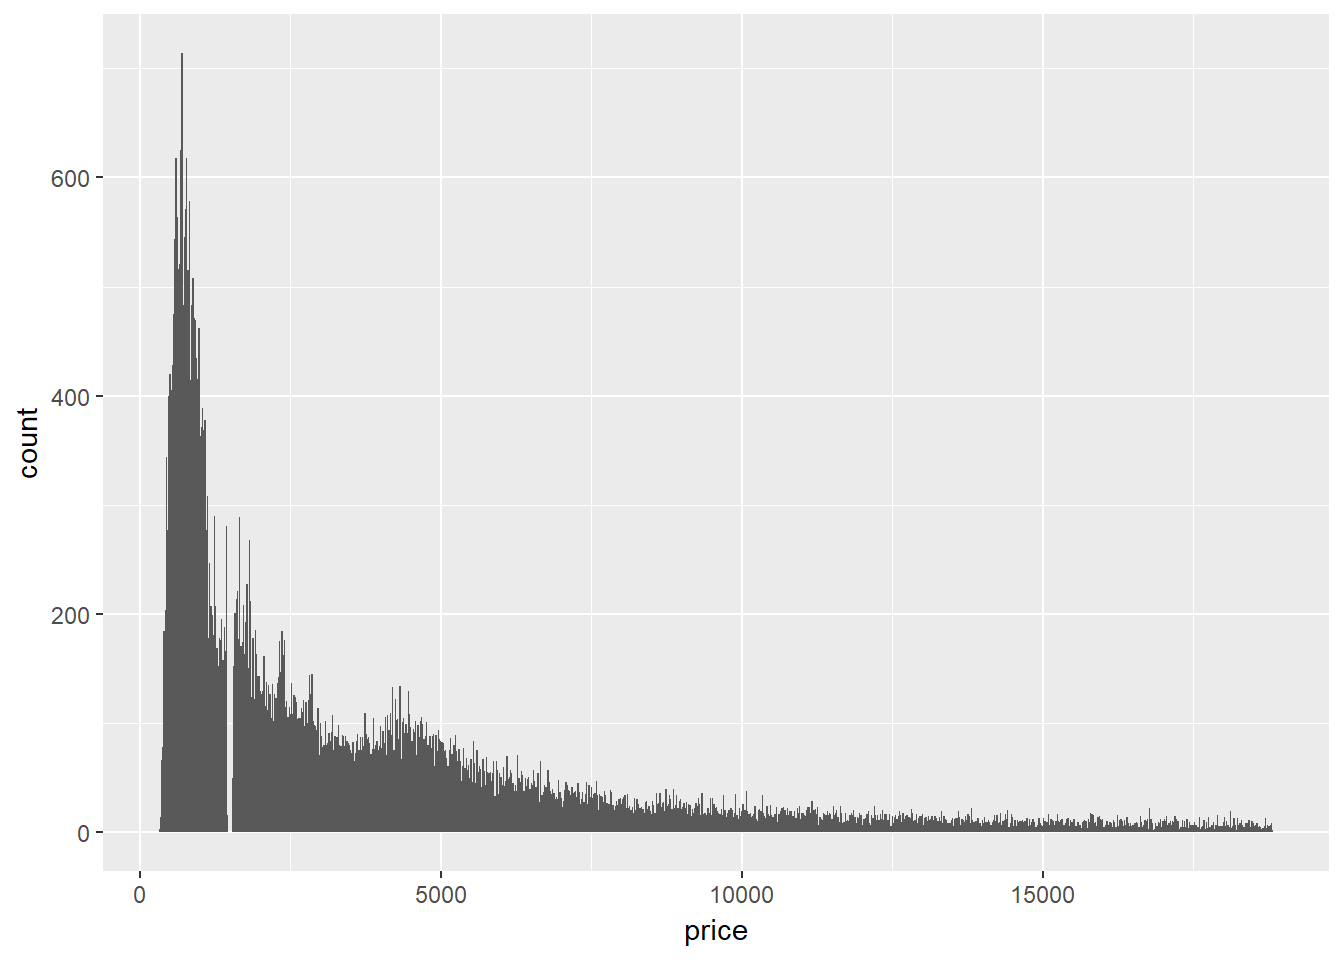
\includegraphics{R4DS_bookdown_files/figure-latex/unnamed-chunk-109-1.pdf}

\emph{3 - How many diamonds are 0.99 carat? How many are 1 carat? What
do you think is the cause of the difference?}

\begin{Shaded}
\begin{Highlighting}[]
\NormalTok{diamonds }\OperatorTok\StringTok{ }\KeywordTok{filter}\NormalTok{(}\KeywordTok{between}\NormalTok{(carat, .}\DecValTok{96}\NormalTok{, }\FloatTok{1.05}\NormalTok{)) }\OperatorTok
\StringTok{  }\KeywordTok{group_by}\NormalTok{(carat) }\OperatorTok\StringTok{ }\KeywordTok{summarize}\NormalTok{(}\DataTypeTok{count =} \KeywordTok{n}\NormalTok{())}
\end{Highlighting}
\end{Shaded}

\begin{verbatim}
## # A tibble: 10 x 2
##    carat count
##    <dbl> <int>
##  1 0.960   103
##  2 0.970    59
##  3 0.980    31
##  4 0.990    23
##  5 1.00   1558
##  6 1.01   2242
##  7 1.02    883
##  8 1.03    523
##  9 1.04    475
## 10 1.05    361
\end{verbatim}

I am no diamond expert, but the data shows that there are way more 1ct
diamonds than .99ct diamonds. (It could be the tendency of humans to
report rounded numbers.)

\emph{4 - Compare and contrast \texttt{coord\_cartesian()} vs
\texttt{xlim()} or \texttt{ylim()} when zooming in on a histogram. What
happens if you leave \texttt{binwidth} unset? What happens if you try
and zoom so only half a bar shows?}

Let's compare the difference between the functions when we set the x
limits to 0 and 5000 and y limits to 0 and 700. We use the same
histogram from the last question and leave the \texttt{binwidth} to 20.

Using \texttt{coord\_cartesian}:

\begin{Shaded}
\begin{Highlighting}[]
\KeywordTok{ggplot}\NormalTok{(}\DataTypeTok{data =}\NormalTok{ diamonds) }\OperatorTok{+}
\StringTok{  }\KeywordTok{geom_histogram}\NormalTok{(}\DataTypeTok{mapping =} \KeywordTok{aes}\NormalTok{(}\DataTypeTok{x =}\NormalTok{ price), }\DataTypeTok{binwidth =} \DecValTok{20}\NormalTok{) }\OperatorTok{+}
\StringTok{  }\KeywordTok{coord_cartesian}\NormalTok{(}\DataTypeTok{xlim =} \KeywordTok{c}\NormalTok{(}\DecValTok{0}\NormalTok{,}\DecValTok{5000}\NormalTok{), }\DataTypeTok{ylim =} \KeywordTok{c}\NormalTok{(}\DecValTok{0}\NormalTok{,}\DecValTok{700}\NormalTok{))}
\end{Highlighting}
\end{Shaded}

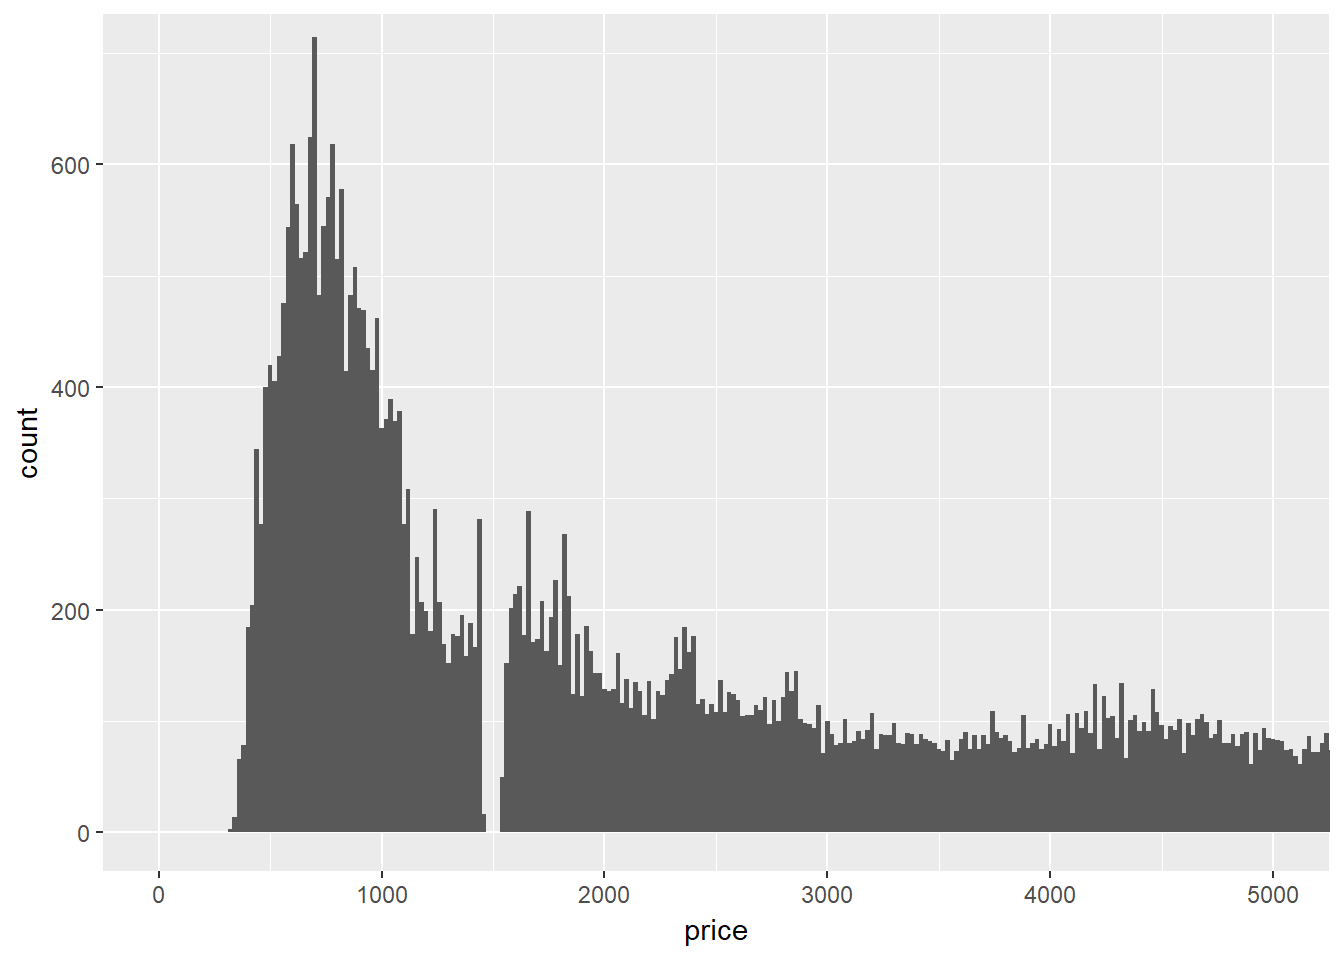
\includegraphics{R4DS_bookdown_files/figure-latex/unnamed-chunk-111-1.pdf}

One thing to notice that even the x and y limit are set to 5000 and 700
respectively, some data beyond those limits are still being shown. We
can override this behavior with \texttt{expand\ =\ FALSE}.

\texttt{xlim()} and \texttt{ylim()}:

\begin{Shaded}
\begin{Highlighting}[]
\KeywordTok{ggplot}\NormalTok{(}\DataTypeTok{data =}\NormalTok{ diamonds) }\OperatorTok{+}
\StringTok{  }\KeywordTok{geom_histogram}\NormalTok{(}\DataTypeTok{mapping =} \KeywordTok{aes}\NormalTok{(}\DataTypeTok{x =}\NormalTok{ price), }\DataTypeTok{binwidth =} \DecValTok{20}\NormalTok{) }\OperatorTok{+}
\StringTok{  }\KeywordTok{xlim}\NormalTok{(}\KeywordTok{c}\NormalTok{(}\DecValTok{0}\NormalTok{,}\DecValTok{5000}\NormalTok{)) }\OperatorTok{+}
\StringTok{  }\KeywordTok{ylim}\NormalTok{(}\KeywordTok{c}\NormalTok{(}\DecValTok{0}\NormalTok{,}\DecValTok{700}\NormalTok{))}
\end{Highlighting}
\end{Shaded}

\begin{verbatim}
## Warning: Removed 14714 rows containing non-finite values (stat_bin).
\end{verbatim}

\begin{verbatim}
## Warning: Removed 1 rows containing missing values (geom_bar).
\end{verbatim}

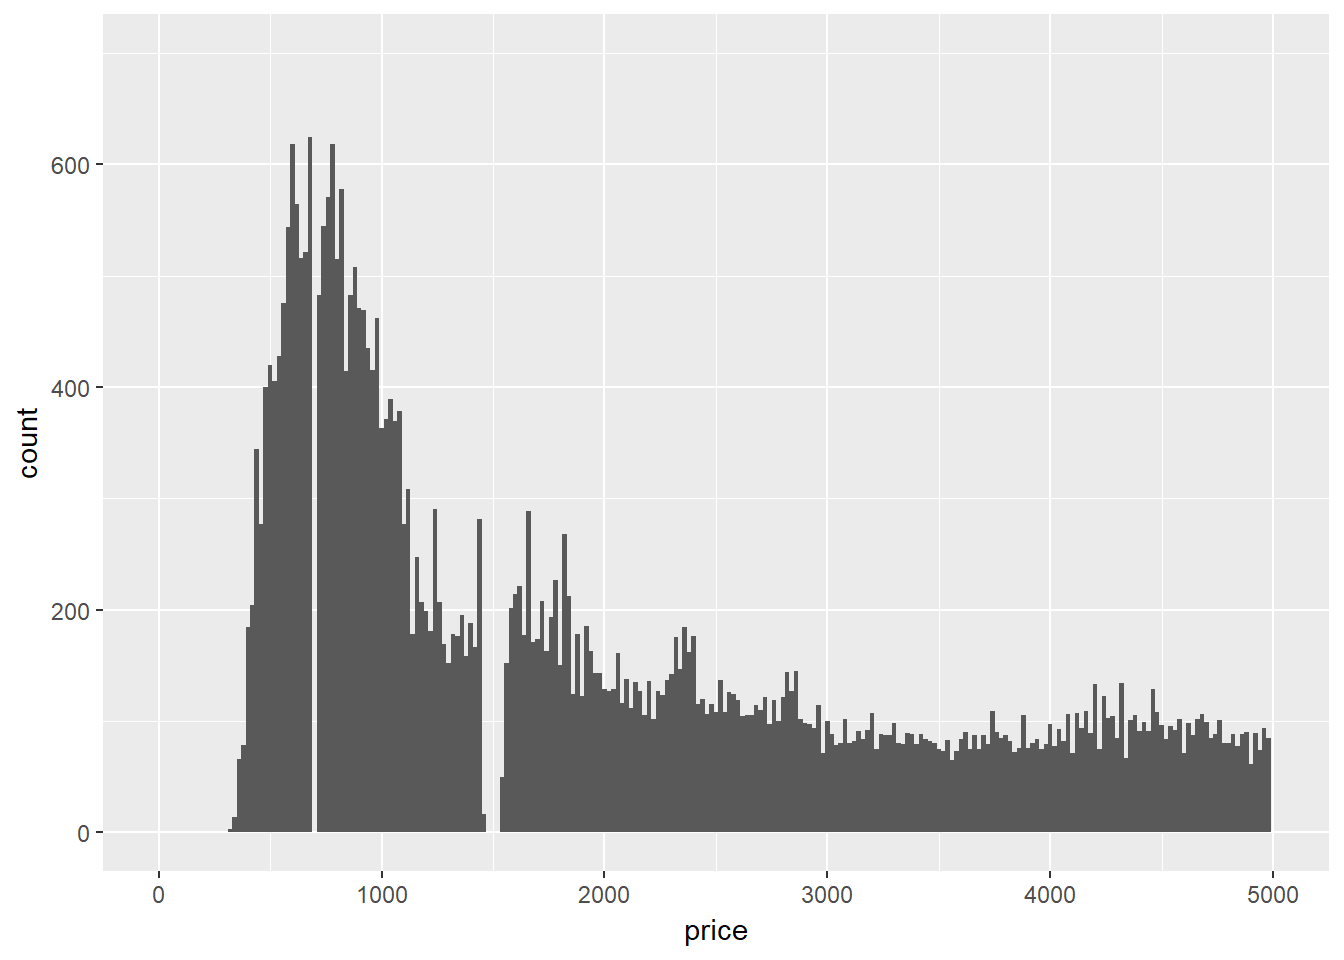
\includegraphics{R4DS_bookdown_files/figure-latex/unnamed-chunk-112-1.pdf}

With \texttt{xlim()} and \texttt{ylim()}, data that are outside of the
limits are not shown. It's fine with the x axis, but do notice that
there is a missing bin at around \$700. For that particular bin, the
height is beyond the y limit of 700.

\subsection{Missing values}\label{missing-values}

\subsubsection{Exercises}\label{exercises-14}

\emph{1 - What happens to missing values in a histogram? What happens to
missing values in a bar chart? Why is there a difference?}

In \texttt{geom\_histogram()}, the missing values are removed.

\begin{Shaded}
\begin{Highlighting}[]
\KeywordTok{data.frame}\NormalTok{(}\DataTypeTok{value =} \KeywordTok{c}\NormalTok{(}\OtherTok{NA}\NormalTok{, }\OtherTok{NA}\NormalTok{, }\OtherTok{NA}\NormalTok{, }\KeywordTok{rnorm}\NormalTok{(}\DecValTok{1000}\NormalTok{,}\DecValTok{0}\NormalTok{,}\DecValTok{1}\NormalTok{))) }\OperatorTok\StringTok{ }\KeywordTok{ggplot}\NormalTok{() }\OperatorTok{+}
\StringTok{  }\KeywordTok{geom_histogram}\NormalTok{(}\DataTypeTok{mapping =} \KeywordTok{aes}\NormalTok{(}\DataTypeTok{x =}\NormalTok{ value), }\DataTypeTok{bins =} \DecValTok{50}\NormalTok{)}
\end{Highlighting}
\end{Shaded}

\begin{verbatim}
## Warning: Removed 3 rows containing non-finite values (stat_bin).
\end{verbatim}

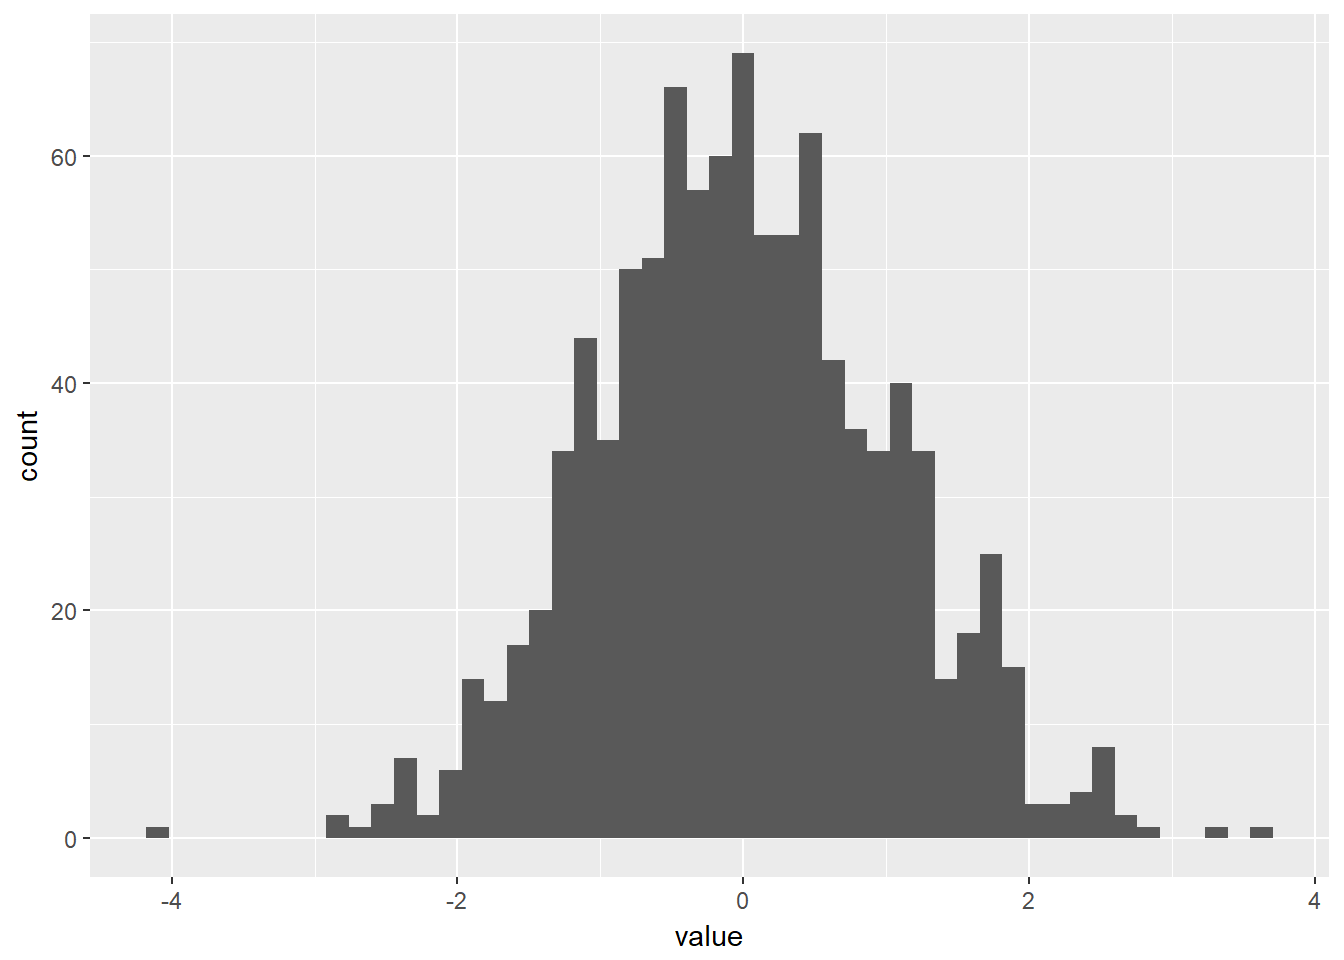
\includegraphics{R4DS_bookdown_files/figure-latex/unnamed-chunk-113-1.pdf}

In \texttt{geom\_bar()}, the missing values are counted and treated as a
category.

\begin{Shaded}
\begin{Highlighting}[]
\KeywordTok{ggplot}\NormalTok{(}\DataTypeTok{data =} \KeywordTok{data.frame}\NormalTok{(}\DataTypeTok{type =} \KeywordTok{c}\NormalTok{(}\StringTok{'A'}\NormalTok{,}\StringTok{'A'}\NormalTok{,}\StringTok{'B'}\NormalTok{,}\StringTok{'B'}\NormalTok{,}\StringTok{'B'}\NormalTok{,}\OtherTok{NA}\NormalTok{))) }\OperatorTok{+}\StringTok{ }
\StringTok{  }\KeywordTok{geom_bar}\NormalTok{(}\DataTypeTok{mapping =} \KeywordTok{aes}\NormalTok{(}\DataTypeTok{x =}\NormalTok{ type))}
\end{Highlighting}
\end{Shaded}

\includegraphics{R4DS_bookdown_files/figure-latex/unnamed-chunk-114-1.pdf}

The reason for the difference is that essentially, histograms are used
for displaying continuous variables, while bar charts are used for
visualizing categorical variables.

\emph{2 - What does \texttt{na.rm\ =\ TRUE} do in \texttt{mean()} and
\texttt{sum()}?}

If there are missing values in the vector, \texttt{mean()} and
\texttt{sum()} will return \texttt{NA}. By including
\texttt{na.rm\ =\ TRUE}, \texttt{mean()} and \texttt{sum()} will return
the average and sum based on the non-missing values in the vector. For
example:

\begin{Shaded}
\begin{Highlighting}[]
\KeywordTok{mean}\NormalTok{(}\KeywordTok{c}\NormalTok{(}\DecValTok{1}\NormalTok{,}\DecValTok{2}\NormalTok{,}\DecValTok{3}\NormalTok{,}\OtherTok{NA}\NormalTok{,}\DecValTok{4}\NormalTok{), }\DataTypeTok{na.rm =} \OtherTok{TRUE}\NormalTok{)}
\end{Highlighting}
\end{Shaded}

\begin{verbatim}
## [1] 2.5
\end{verbatim}

\subsection{Covariation}\label{covariation}

\subsubsection{A categorical and continuous
variable}\label{a-categorical-and-continuous-variable}

\paragraph{Exercises}\label{exercises-15}

\emph{1 - Use what you've learned to improve the visualisation of the
departure times of cancelled vs.~non-cancelled flights.}

The problem with the original visualisation of the departure times of
cancelled vs.~non-cancelled flights is that since there are far less
cancelled flights, the distribution of non-cancelled flights looks flat
when plotted together with non-cancelled flights.

We can use \texttt{freq\_density()} to force the area under each curve
sums up to 1.

\begin{Shaded}
\begin{Highlighting}[]
\NormalTok{nycflights13}\OperatorTok{::}\NormalTok{flights }\OperatorTok\StringTok{ }
\StringTok{  }\KeywordTok{mutate}\NormalTok{(}
    \DataTypeTok{cancelled =} \KeywordTok{is.na}\NormalTok{(dep_time),}
    \DataTypeTok{sched_hour =}\NormalTok{ sched_dep_time }\OperatorTok\StringTok{ }\DecValTok{100}\NormalTok{,}
    \DataTypeTok{sched_min =}\NormalTok{ sched_dep_time }\OperatorTok\StringTok{ }\DecValTok{100}\NormalTok{,}
    \DataTypeTok{sched_dep_time =}\NormalTok{ sched_hour }\OperatorTok{+}\StringTok{ }\NormalTok{sched_min }\OperatorTok{/}\StringTok{ }\DecValTok{60}
\NormalTok{  ) }\OperatorTok\StringTok{ }
\StringTok{  }\KeywordTok{ggplot}\NormalTok{(}\DataTypeTok{mapping =} \KeywordTok{aes}\NormalTok{(sched_dep_time)) }\OperatorTok{+}\StringTok{ }
\StringTok{    }\KeywordTok{geom_density}\NormalTok{(}\DataTypeTok{mapping =} \KeywordTok{aes}\NormalTok{(}\DataTypeTok{colour =}\NormalTok{ cancelled))}
\end{Highlighting}
\end{Shaded}

\includegraphics{R4DS_bookdown_files/figure-latex/unnamed-chunk-116-1.pdf}

Or we can use \texttt{geom\_boxplot()}.

\begin{Shaded}
\begin{Highlighting}[]
\NormalTok{nycflights13}\OperatorTok{::}\NormalTok{flights }\OperatorTok\StringTok{ }
\StringTok{  }\KeywordTok{mutate}\NormalTok{(}
    \DataTypeTok{cancelled =} \KeywordTok{is.na}\NormalTok{(dep_time),}
    \DataTypeTok{sched_hour =}\NormalTok{ sched_dep_time }\OperatorTok\StringTok{ }\DecValTok{100}\NormalTok{,}
    \DataTypeTok{sched_min =}\NormalTok{ sched_dep_time }\OperatorTok\StringTok{ }\DecValTok{100}\NormalTok{,}
    \DataTypeTok{sched_dep_time =}\NormalTok{ sched_hour }\OperatorTok{+}\StringTok{ }\NormalTok{sched_min }\OperatorTok{/}\StringTok{ }\DecValTok{60}
\NormalTok{  ) }\OperatorTok\StringTok{ }
\StringTok{  }\KeywordTok{ggplot}\NormalTok{() }\OperatorTok{+}
\StringTok{  }\KeywordTok{geom_boxplot}\NormalTok{(}\DataTypeTok{mapping =} \KeywordTok{aes}\NormalTok{(}\DataTypeTok{x =}\NormalTok{ cancelled, }\DataTypeTok{y =}\NormalTok{ sched_dep_time))}
\end{Highlighting}
\end{Shaded}

\includegraphics{R4DS_bookdown_files/figure-latex/unnamed-chunk-117-1.pdf}

\emph{2 - What variable in the diamonds dataset is most important for
predicting the price of a diamond? How is that variable correlated with
cut? Why does the combination of those two relationships lead to lower
quality diamonds being more expensive?}

Since \texttt{cut}, \texttt{color}, and \texttt{clarity} are ordered
categorical variables, I made an assumption that they could be treated
as continuous variables. Checking the correlation matrix:

\begin{Shaded}
\begin{Highlighting}[]
\NormalTok{diamonds }\OperatorTok
\StringTok{  }\KeywordTok{mutate}\NormalTok{(}\DataTypeTok{cut =} \KeywordTok{as.numeric}\NormalTok{(cut),}
         \DataTypeTok{color =} \KeywordTok{as.numeric}\NormalTok{(color),}
         \DataTypeTok{clarity =} \KeywordTok{as.numeric}\NormalTok{(clarity)) }\OperatorTok
\StringTok{  }\KeywordTok{select}\NormalTok{(price, }\KeywordTok{everything}\NormalTok{()) }\OperatorTok
\StringTok{  }\KeywordTok{cor}\NormalTok{()}
\end{Highlighting}
\end{Shaded}

\begin{verbatim}
##               price       carat         cut       color     clarity
## price    1.00000000  0.92159130 -0.05349066  0.17251093 -0.14680007
## carat    0.92159130  1.00000000 -0.13496702  0.29143675 -0.35284057
## cut     -0.05349066 -0.13496702  1.00000000 -0.02051852  0.18917474
## color    0.17251093  0.29143675 -0.02051852  1.00000000  0.02563128
## clarity -0.14680007 -0.35284057  0.18917474  0.02563128  1.00000000
## depth   -0.01064740  0.02822431 -0.21805501  0.04727923 -0.06738444
## table    0.12713390  0.18161755 -0.43340461  0.02646520 -0.16032684
## x        0.88443516  0.97509423 -0.12556524  0.27028669 -0.37199853
## y        0.86542090  0.95172220 -0.12146187  0.26358440 -0.35841962
## z        0.86124944  0.95338738 -0.14932254  0.26822688 -0.36695200
##               depth      table           x           y           z
## price   -0.01064740  0.1271339  0.88443516  0.86542090  0.86124944
## carat    0.02822431  0.1816175  0.97509423  0.95172220  0.95338738
## cut     -0.21805501 -0.4334046 -0.12556524 -0.12146187 -0.14932254
## color    0.04727923  0.0264652  0.27028669  0.26358440  0.26822688
## clarity -0.06738444 -0.1603268 -0.37199853 -0.35841962 -0.36695200
## depth    1.00000000 -0.2957785 -0.02528925 -0.02934067  0.09492388
## table   -0.29577852  1.0000000  0.19534428  0.18376015  0.15092869
## x       -0.02528925  0.1953443  1.00000000  0.97470148  0.97077180
## y       -0.02934067  0.1837601  0.97470148  1.00000000  0.95200572
## z        0.09492388  0.1509287  0.97077180  0.95200572  1.00000000
\end{verbatim}

\texttt{carat} is the most correlated variable with \texttt{price}, so
it is the most important variable in predicting price of diamonds.

\texttt{carat} and \texttt{cut} are slightly negatively correlated,
meaning diamonds of higher weights tend to have a lower cut rating.

To answer the last question, we run an ordinary linear regression with
\texttt{carat}, \texttt{cut} and \texttt{carat*cut}, the interaction
effect, on \texttt{price}.

\begin{Shaded}
\begin{Highlighting}[]
\NormalTok{diamonds_con <-}\StringTok{ }\NormalTok{diamonds }\OperatorTok
\StringTok{  }\KeywordTok{mutate}\NormalTok{(}\DataTypeTok{cut =} \KeywordTok{as.numeric}\NormalTok{(cut),}
         \DataTypeTok{color =} \KeywordTok{as.numeric}\NormalTok{(color),}
         \DataTypeTok{clarity =} \KeywordTok{as.numeric}\NormalTok{(clarity))}

\KeywordTok{summary}\NormalTok{(}\KeywordTok{lm}\NormalTok{(price }\OperatorTok{~}\StringTok{ }\NormalTok{carat }\OperatorTok{+}\StringTok{ }\NormalTok{cut }\OperatorTok{+}\StringTok{ }\NormalTok{carat}\OperatorTok{*}\NormalTok{cut, }\DataTypeTok{data =}\NormalTok{ diamonds_con))}
\end{Highlighting}
\end{Shaded}

\begin{verbatim}
## 
## Call:
## lm(formula = price ~ carat + cut + carat * cut, data = diamonds_con)
## 
## Residuals:
##      Min       1Q   Median       3Q      Max 
## -14108.3   -779.4    -24.8    536.4  12983.9 
## 
## Coefficients:
##             Estimate Std. Error t value Pr(>|t|)    
## (Intercept) -2194.59      48.54 -45.209   <2e-16 ***
## carat        6491.28      49.43 131.321   <2e-16 ***
## cut           -30.26      11.73  -2.579   0.0099 ** 
## carat:cut     350.18      12.33  28.391   <2e-16 ***
## ---
## Signif. codes:  0 '***' 0.001 '**' 0.01 '*' 0.05 '.' 0.1 ' ' 1
## 
## Residual standard error: 1511 on 53936 degrees of freedom
## Multiple R-squared:  0.8566, Adjusted R-squared:  0.8566 
## F-statistic: 1.074e+05 on 3 and 53936 DF,  p-value: < 2.2e-16
\end{verbatim}

The main effect of \texttt{cut} is -30.26, it does show over and above
the effects of carat and the interaction between carat and cut, that
higher cut quality leads to lower price. However, in the presense of a
highly significant interaction effect, we need to interpret the main
effect with interaction effect. Rearanging terms, we get
\texttt{price\ =\ cut\ *\ (-30.26\ +\ 350.18\ *\ carat)\ +\ 6491.28\ *\ carat}.
Higher cut quality actually does lead to a higher price.

\emph{3 - Install the ggstance package, and create a horizontal boxplot.
How does this compare to using \texttt{coord\_flip()?}}

We can just simply add 'coord\_flip()` to make the boxplot to be shown
horizontally:

\begin{Shaded}
\begin{Highlighting}[]
\NormalTok{nycflights13}\OperatorTok{::}\NormalTok{flights }\OperatorTok\StringTok{ }
\StringTok{  }\KeywordTok{mutate}\NormalTok{(}
    \DataTypeTok{cancelled =} \KeywordTok{is.na}\NormalTok{(dep_time),}
    \DataTypeTok{sched_hour =}\NormalTok{ sched_dep_time }\OperatorTok\StringTok{ }\DecValTok{100}\NormalTok{,}
    \DataTypeTok{sched_min =}\NormalTok{ sched_dep_time }\OperatorTok\StringTok{ }\DecValTok{100}\NormalTok{,}
    \DataTypeTok{sched_dep_time =}\NormalTok{ sched_hour }\OperatorTok{+}\StringTok{ }\NormalTok{sched_min }\OperatorTok{/}\StringTok{ }\DecValTok{60}
\NormalTok{  ) }\OperatorTok\StringTok{ }
\StringTok{  }\KeywordTok{ggplot}\NormalTok{() }\OperatorTok{+}
\StringTok{  }\KeywordTok{geom_boxplot}\NormalTok{(}\DataTypeTok{mapping =} \KeywordTok{aes}\NormalTok{(}\DataTypeTok{x =}\NormalTok{ cancelled, }\DataTypeTok{y =}\NormalTok{ sched_dep_time)) }\OperatorTok{+}
\StringTok{  }\KeywordTok{coord_flip}\NormalTok{()}
\end{Highlighting}
\end{Shaded}

\includegraphics{R4DS_bookdown_files/figure-latex/unnamed-chunk-120-1.pdf}

However, when using \texttt{geom\_boxploth()} from \texttt{ggstance},
the \texttt{x} and \texttt{y} in \texttt{mapping} need to be switched.

\begin{Shaded}
\begin{Highlighting}[]
\KeywordTok{library}\NormalTok{(ggstance)}
\NormalTok{nycflights13}\OperatorTok{::}\NormalTok{flights }\OperatorTok\StringTok{ }
\StringTok{  }\KeywordTok{mutate}\NormalTok{(}
    \DataTypeTok{cancelled =} \KeywordTok{is.na}\NormalTok{(dep_time),}
    \DataTypeTok{sched_hour =}\NormalTok{ sched_dep_time }\OperatorTok\StringTok{ }\DecValTok{100}\NormalTok{,}
    \DataTypeTok{sched_min =}\NormalTok{ sched_dep_time }\OperatorTok\StringTok{ }\DecValTok{100}\NormalTok{,}
    \DataTypeTok{sched_dep_time =}\NormalTok{ sched_hour }\OperatorTok{+}\StringTok{ }\NormalTok{sched_min }\OperatorTok{/}\StringTok{ }\DecValTok{60}
\NormalTok{  ) }\OperatorTok\StringTok{ }
\StringTok{  }\KeywordTok{ggplot}\NormalTok{() }\OperatorTok{+}
\StringTok{  }\KeywordTok{geom_boxploth}\NormalTok{(}\DataTypeTok{mapping =} \KeywordTok{aes}\NormalTok{(}\DataTypeTok{y =}\NormalTok{ cancelled, }\DataTypeTok{x =}\NormalTok{ sched_dep_time))}
\end{Highlighting}
\end{Shaded}

\includegraphics{R4DS_bookdown_files/figure-latex/unnamed-chunk-121-1.pdf}

\emph{4 - One problem with boxplots is that they were developed in an
era of much smaller datasets and tend to display a prohibitively large
number of outlying values. One approach to remedy this problem is the
letter value plot. Install the lvplot package, and try using
\texttt{geom\_lv()} to display the distribution of price vs cut. What do
you learn? How do you interpret the plots?}

As stated in the problem, the traditional boxplot displays a large
number of outliers:

\begin{Shaded}
\begin{Highlighting}[]
\KeywordTok{ggplot}\NormalTok{(}\DataTypeTok{data =}\NormalTok{ diamonds) }\OperatorTok{+}
\StringTok{  }\KeywordTok{geom_boxplot}\NormalTok{(}\DataTypeTok{mapping =} \KeywordTok{aes}\NormalTok{(}\DataTypeTok{x =}\NormalTok{ cut, }\DataTypeTok{y =}\NormalTok{ price))}
\end{Highlighting}
\end{Shaded}

\includegraphics{R4DS_bookdown_files/figure-latex/unnamed-chunk-122-1.pdf}

A letter value plot:

\begin{Shaded}
\begin{Highlighting}[]
\KeywordTok{library}\NormalTok{(lvplot)}

\KeywordTok{ggplot}\NormalTok{(}\DataTypeTok{data =}\NormalTok{ diamonds) }\OperatorTok{+}
\StringTok{  }\KeywordTok{geom_lv}\NormalTok{(}\DataTypeTok{mapping =} \KeywordTok{aes}\NormalTok{(}\DataTypeTok{x =}\NormalTok{ cut, }\DataTypeTok{y =}\NormalTok{ price))}
\end{Highlighting}
\end{Shaded}

\includegraphics{R4DS_bookdown_files/figure-latex/unnamed-chunk-123-1.pdf}

Interpretations - To Do.

\emph{5 - Compare and contrast \texttt{geom\_violin()} with a facetted
\texttt{geom\_histogram()}, or a coloured \texttt{geom\_freqpoly()}.
What are the pros and cons of each method?}

Facetted histograms:

\begin{Shaded}
\begin{Highlighting}[]
\NormalTok{diamonds }\OperatorTok\StringTok{ }\KeywordTok{ggplot}\NormalTok{() }\OperatorTok{+}
\StringTok{  }\KeywordTok{geom_histogram}\NormalTok{(}\DataTypeTok{mapping =} \KeywordTok{aes}\NormalTok{(}\DataTypeTok{x =}\NormalTok{ price), }\DataTypeTok{binwidth =} \DecValTok{50}\NormalTok{) }\OperatorTok{+}
\StringTok{  }\KeywordTok{facet_grid}\NormalTok{(cut}\OperatorTok{~}\NormalTok{.)}
\end{Highlighting}
\end{Shaded}

\includegraphics{R4DS_bookdown_files/figure-latex/unnamed-chunk-124-1.pdf}

By default, a facetted plot has fixed x and y scale. In this case, it is
hard to see the distribution of price for fair diamonds because there
are far less fair diamonds compared with the others. We are free the y
scale by adding
\texttt{scales\ =\ \textquotesingle{}free\_y\textquotesingle{}} in
\texttt{facet\_grid}. However, doing so will make the histograms less
comparable in a sense that they will have different y scale.

Another point about histogram is that the shape and appearance is
sensitive to the number of \texttt{bins} or \texttt{binwidth}.

\texttt{geom\_violin()}:

\begin{Shaded}
\begin{Highlighting}[]
\NormalTok{diamonds }\OperatorTok\StringTok{ }\KeywordTok{ggplot}\NormalTok{() }\OperatorTok{+}
\StringTok{  }\KeywordTok{geom_violin}\NormalTok{(}\DataTypeTok{mapping =} \KeywordTok{aes}\NormalTok{(}\DataTypeTok{x =}\NormalTok{ cut, }\DataTypeTok{y =}\NormalTok{ price))}
\end{Highlighting}
\end{Shaded}

\includegraphics{R4DS_bookdown_files/figure-latex/unnamed-chunk-125-1.pdf}

The violin plot displays a compact view of continuous distributions. The
curve in the violion is actually a probabilty density function, so the
area always sums up to 1 (or 2 if you consider the mirrored part).
However, it does not give us the information of which cut of diamonds
are more or less abundant than others.

\texttt{geom\_freqpoly}:

\begin{Shaded}
\begin{Highlighting}[]
\NormalTok{diamonds }\OperatorTok\StringTok{ }\KeywordTok{ggplot}\NormalTok{() }\OperatorTok{+}
\StringTok{  }\KeywordTok{geom_freqpoly}\NormalTok{(}\DataTypeTok{mapping =} \KeywordTok{aes}\NormalTok{(}\DataTypeTok{x =}\NormalTok{ price, }\DataTypeTok{color =}\NormalTok{ cut), }\DataTypeTok{binwidth =} \DecValTok{50}\NormalTok{)}
\end{Highlighting}
\end{Shaded}

\includegraphics{R4DS_bookdown_files/figure-latex/unnamed-chunk-126-1.pdf}

Similiar to factted histogram, except they are represented as freqploy
and plotted on the same graph.

\emph{6 - If you have a small dataset, it's sometimes useful to use
\texttt{geom\_jitter()} to see the relationship between a continuous and
categorical variable. The ggbeeswarm package provides a number of
methods similar to \texttt{geom\_jitter()}. List them and briefly
describe what each one does.}

\begin{Shaded}
\begin{Highlighting}[]
\KeywordTok{ggplot}\NormalTok{(}\DataTypeTok{data =}\NormalTok{ mpg) }\OperatorTok{+}\StringTok{ }
\StringTok{  }\KeywordTok{geom_jitter}\NormalTok{(}\DataTypeTok{mapping =} \KeywordTok{aes}\NormalTok{(}\DataTypeTok{x =}\NormalTok{ drv, }\DataTypeTok{y =}\NormalTok{ displ))}
\end{Highlighting}
\end{Shaded}

\includegraphics{R4DS_bookdown_files/figure-latex/unnamed-chunk-127-1.pdf}

\texttt{geom\_jitter()} slightly shifts the data horizontally and
vertically randomly to overcome overplotting.

\begin{Shaded}
\begin{Highlighting}[]
\KeywordTok{library}\NormalTok{(ggbeeswarm)}

\KeywordTok{ggplot}\NormalTok{(}\DataTypeTok{data =}\NormalTok{ mpg) }\OperatorTok{+}\StringTok{ }
\StringTok{  }\KeywordTok{geom_beeswarm}\NormalTok{(}\DataTypeTok{mapping =} \KeywordTok{aes}\NormalTok{(}\DataTypeTok{x =}\NormalTok{ drv, }\DataTypeTok{y =}\NormalTok{ displ), }\DataTypeTok{priority =} \StringTok{'ascending'}\NormalTok{)}
\end{Highlighting}
\end{Shaded}

\includegraphics{R4DS_bookdown_files/figure-latex/unnamed-chunk-128-1.pdf}

\texttt{geom\_beeswarm()} is another way to overcome overplotting.
Instead of adding random variations along the x and y axis, it ``lines
up'' the data points and also shows the distribution.

\subsubsection{Two categorical
variables}\label{two-categorical-variables}

\paragraph{Exercises}\label{exercises-16}

\emph{1 - How could you rescale the count dataset above to more clearly
show the distribution of cut within colour, or colour within cut?}

The original plot shows the counts for each combination of \texttt{cut}
and \texttt{color}. Since both \texttt{cut} and \texttt{color} are
categorical variables, we cannot use \texttt{geom\_density()} to show
the distribtuion of \texttt{cut} within \texttt{color}, or
\texttt{color} with \texttt{cut}. Instead, we can calculate the
proportion of each \texttt{cut} within \texttt{color}, and vice versa.

Here, we rescale the dataset and show the distribution of \texttt{cut}
within \texttt{color}:

\begin{Shaded}
\begin{Highlighting}[]
\NormalTok{diamonds }\OperatorTok\StringTok{ }\KeywordTok{count}\NormalTok{(color, cut) }\OperatorTok\StringTok{ }\KeywordTok{group_by}\NormalTok{(color) }\OperatorTok
\StringTok{  }\KeywordTok{mutate}\NormalTok{(}\DataTypeTok{prop =}\NormalTok{ n }\OperatorTok{/}\StringTok{ }\KeywordTok{sum}\NormalTok{(n)) }\OperatorTok
\StringTok{  }\KeywordTok{ggplot}\NormalTok{() }\OperatorTok{+}
\StringTok{  }\KeywordTok{geom_tile}\NormalTok{(}\DataTypeTok{mapping =} \KeywordTok{aes}\NormalTok{(}\DataTypeTok{x =}\NormalTok{ color, }\DataTypeTok{y =}\NormalTok{ cut, }\DataTypeTok{fill =}\NormalTok{ prop)) }\OperatorTok{+}
\StringTok{  }\KeywordTok{labs}\NormalTok{(}\DataTypeTok{title =} \StringTok{'Distribution of cut within color'}\NormalTok{)}
\end{Highlighting}
\end{Shaded}

\includegraphics{R4DS_bookdown_files/figure-latex/unnamed-chunk-129-1.pdf}

\emph{2 - Use \texttt{geom\_tile()} together with dplyr to explore how
average flight delays vary by destination and month of year. What makes
the plot difficult to read? How could you improve it?}

\begin{Shaded}
\begin{Highlighting}[]
\NormalTok{nycflights13}\OperatorTok{::}\NormalTok{flights }\OperatorTok\StringTok{ }\KeywordTok{group_by}\NormalTok{(dest, month) }\OperatorTok
\StringTok{  }\KeywordTok{summarize}\NormalTok{(}\DataTypeTok{avg_dep_delay =} \KeywordTok{mean}\NormalTok{(dep_delay, }\DataTypeTok{na.rm =} \OtherTok{TRUE}\NormalTok{)) }\OperatorTok
\StringTok{  }\KeywordTok{ggplot}\NormalTok{() }\OperatorTok{+}
\StringTok{  }\KeywordTok{geom_tile}\NormalTok{(}\DataTypeTok{mapping =} \KeywordTok{aes}\NormalTok{(}\DataTypeTok{x =}\NormalTok{ month, }\DataTypeTok{y =}\NormalTok{ dest, }\DataTypeTok{fill =}\NormalTok{ avg_dep_delay))}
\end{Highlighting}
\end{Shaded}

\includegraphics{R4DS_bookdown_files/figure-latex/unnamed-chunk-130-1.pdf}

The plot is not easy to read because:

\begin{itemize}
\tightlist
\item
  the color scale range makes it hard to distinguish and compare
  airports and months
\item
  there are empty cells, which denote missing values (no flights
  departed from the airport, different from averaged delayed in 0
  minutes)
\item
  the x label is incorrect
\end{itemize}

We will keep the NA cells for two reasons:

\begin{itemize}
\tightlist
\item
  not ideal if we remove the entire row. The non-missing cells still
  represent data.
\item
  NA actually reflects that no flights departed in the origin airports
  in that particular month (which is odd, but that's the data we are
  given). Let's just assumme it means something.
\end{itemize}

We will arrange the plot so that airports with missing months will be
shown at the bottom, and manually set the gradient scale:

\begin{Shaded}
\begin{Highlighting}[]
\NormalTok{nycflights13}\OperatorTok{::}\NormalTok{flights }\OperatorTok\StringTok{ }\KeywordTok{group_by}\NormalTok{(dest, month) }\OperatorTok
\StringTok{  }\KeywordTok{summarize}\NormalTok{(}\DataTypeTok{avg_dep_delay =} \KeywordTok{mean}\NormalTok{(dep_delay, }\DataTypeTok{na.rm =} \OtherTok{TRUE}\NormalTok{)) }\OperatorTok
\StringTok{  }\KeywordTok{ungroup}\NormalTok{() }\OperatorTok
\StringTok{  }\KeywordTok{group_by}\NormalTok{(dest) }\OperatorTok
\StringTok{  }\KeywordTok{mutate}\NormalTok{(}\DataTypeTok{n_month =} \KeywordTok{n}\NormalTok{())}\OperatorTok
\StringTok{  }\KeywordTok{ggplot}\NormalTok{() }\OperatorTok{+}
\StringTok{  }\KeywordTok{geom_tile}\NormalTok{(}\DataTypeTok{mapping =} \KeywordTok{aes}\NormalTok{(}\DataTypeTok{x =} \KeywordTok{factor}\NormalTok{(month),}
                          \DataTypeTok{y =} \KeywordTok{reorder}\NormalTok{(dest, n_month),}
                          \DataTypeTok{fill =}\NormalTok{ avg_dep_delay)) }\OperatorTok{+}
\StringTok{  }\KeywordTok{scale_fill_gradient2}\NormalTok{(}\DataTypeTok{low =} \StringTok{'yellow'}\NormalTok{, }\DataTypeTok{mid =} \StringTok{'orange'}\NormalTok{, }\DataTypeTok{high =} \StringTok{'red'}\NormalTok{,}
                       \DataTypeTok{midpoint =} \DecValTok{35}\NormalTok{)}
\end{Highlighting}
\end{Shaded}

\includegraphics{R4DS_bookdown_files/figure-latex/unnamed-chunk-131-1.pdf}

\emph{3 - Why is it slightly better to use
\texttt{aes(x\ =\ color,\ y\ =\ cut)} rather than
\texttt{aes(x\ =\ cut,\ y\ =\ color)} in the example above?}

\begin{Shaded}
\begin{Highlighting}[]
\NormalTok{diamonds }\OperatorTok\StringTok{ }\KeywordTok{count}\NormalTok{(color, cut) }\OperatorTok\StringTok{ }\KeywordTok{group_by}\NormalTok{(color) }\OperatorTok
\StringTok{  }\KeywordTok{mutate}\NormalTok{(}\DataTypeTok{prop =}\NormalTok{ n }\OperatorTok{/}\StringTok{ }\KeywordTok{sum}\NormalTok{(n)) }\OperatorTok
\StringTok{  }\KeywordTok{ggplot}\NormalTok{() }\OperatorTok{+}
\StringTok{  }\KeywordTok{geom_tile}\NormalTok{(}\DataTypeTok{mapping =} \KeywordTok{aes}\NormalTok{(}\DataTypeTok{x =}\NormalTok{ cut, }\DataTypeTok{y =}\NormalTok{ color, }\DataTypeTok{fill =}\NormalTok{ prop)) }\OperatorTok{+}
\StringTok{  }\KeywordTok{labs}\NormalTok{(}\DataTypeTok{title =} \StringTok{'Distribution of cut within color'}\NormalTok{)}
\end{Highlighting}
\end{Shaded}

\includegraphics{R4DS_bookdown_files/figure-latex/unnamed-chunk-132-1.pdf}

\subsubsection{Two continuous variables}\label{two-continuous-variables}

\paragraph{Exercises}\label{exercises-17}

\emph{1 - Instead of summarising the conditional distribution with a
boxplot, you could use a frequency polygon. What do you need to consider
when using \texttt{cut\_width()} vs \texttt{cut\_number()}? How does
that impact a visualisation of the 2d distribution of \texttt{carat} and
\texttt{price}?}

Unlike \texttt{geom\_density()}, \texttt{geom\_freqpoly()} is a
smoothered histogram, so the height of each polygon is affected by the
number of observations in each group. Setting the \texttt{cut\_width}
too small will have too many categories. Some of the categories will
have very few observations, resulting in polygons that are flat and
close to the x-axis. Compare the \texttt{cut\_width} of .2 and .4:

\begin{Shaded}
\begin{Highlighting}[]
\NormalTok{diamonds }\OperatorTok\StringTok{ }\KeywordTok{ggplot}\NormalTok{() }\OperatorTok{+}
\StringTok{  }\KeywordTok{geom_freqpoly}\NormalTok{(}\DataTypeTok{mapping =} \KeywordTok{aes}\NormalTok{(}\DataTypeTok{x =}\NormalTok{ price,}
                              \DataTypeTok{color =} \KeywordTok{cut_width}\NormalTok{(carat, .}\DecValTok{2}\NormalTok{)), }\DataTypeTok{bins =} \DecValTok{30}\NormalTok{)}
\end{Highlighting}
\end{Shaded}

\includegraphics{R4DS_bookdown_files/figure-latex/unnamed-chunk-133-1.pdf}

\begin{Shaded}
\begin{Highlighting}[]
\NormalTok{diamonds }\OperatorTok\StringTok{ }\KeywordTok{ggplot}\NormalTok{() }\OperatorTok{+}
\StringTok{  }\KeywordTok{geom_freqpoly}\NormalTok{(}\DataTypeTok{mapping =} \KeywordTok{aes}\NormalTok{(}\DataTypeTok{x =}\NormalTok{ price,}
                              \DataTypeTok{color =} \KeywordTok{cut_width}\NormalTok{(carat, .}\DecValTok{4}\NormalTok{)), }\DataTypeTok{bins =} \DecValTok{30}\NormalTok{)}
\end{Highlighting}
\end{Shaded}

\includegraphics{R4DS_bookdown_files/figure-latex/unnamed-chunk-134-1.pdf}

Since most of the diamonds are below 1 carat, in both plots, the
polygons of above 1 carat are flat, and some are not distingushable from
others.

In contrast, \texttt{cut\_number()} ensures the same number of
observations in each group.

\begin{Shaded}
\begin{Highlighting}[]
\NormalTok{diamonds }\OperatorTok\StringTok{ }\KeywordTok{ggplot}\NormalTok{() }\OperatorTok{+}
\StringTok{  }\KeywordTok{geom_freqpoly}\NormalTok{(}\DataTypeTok{mapping =} \KeywordTok{aes}\NormalTok{(}\DataTypeTok{x =}\NormalTok{ price,}
                              \DataTypeTok{color =} \KeywordTok{cut_number}\NormalTok{(carat, }\DecValTok{10}\NormalTok{)), }\DataTypeTok{bins =} \DecValTok{30}\NormalTok{)}
\end{Highlighting}
\end{Shaded}

\includegraphics{R4DS_bookdown_files/figure-latex/unnamed-chunk-135-1.pdf}

\emph{2 - Visualise the distribution of \texttt{carat}, partitioned by
\texttt{price}.}

Using \texttt{geom\_density()} and partitioning by \texttt{price} with
\texttt{cut\_width}, it is not surprising to see that diamonds of higher
carat are associated with higher price in general.

\begin{Shaded}
\begin{Highlighting}[]
\NormalTok{diamonds }\OperatorTok\StringTok{ }\KeywordTok{ggplot}\NormalTok{() }\OperatorTok{+}
\StringTok{  }\KeywordTok{geom_density}\NormalTok{(}\DataTypeTok{mapping =} \KeywordTok{aes}\NormalTok{(}\DataTypeTok{x =}\NormalTok{ carat,}
                             \DataTypeTok{color =} \KeywordTok{cut_width}\NormalTok{(price, }\DecValTok{5000}\NormalTok{, }\DataTypeTok{boundary =} \DecValTok{0}\NormalTok{)))}
\end{Highlighting}
\end{Shaded}

\includegraphics{R4DS_bookdown_files/figure-latex/unnamed-chunk-136-1.pdf}

\emph{3 - How does the price distribution of very large diamonds compare
to small diamonds. Is it as you expect, or does it surprise you?}

\begin{Shaded}
\begin{Highlighting}[]
\NormalTok{diamonds }\OperatorTok\StringTok{ }\NormalTok{ggplot }\OperatorTok{+}
\StringTok{  }\KeywordTok{geom_boxplot}\NormalTok{(}\DataTypeTok{mapping =} \KeywordTok{aes}\NormalTok{(}\DataTypeTok{x =} \KeywordTok{cut_number}\NormalTok{(carat, }\DecValTok{10}\NormalTok{),}
                             \DataTypeTok{y =}\NormalTok{ price)) }\OperatorTok{+}
\StringTok{  }\KeywordTok{coord_flip}\NormalTok{()}
\end{Highlighting}
\end{Shaded}

\includegraphics{R4DS_bookdown_files/figure-latex/unnamed-chunk-137-1.pdf}

The price distribution of very large diamonds are much more variable
than the smaller diamonds. Perhaps other factors, such as cut, clarity,
and color have heavier influence on the price of larger diamonds.

\emph{4 - Combine two of the techniques you've learned to visualise the
combined distribution of cut, carat, and price.}

We can use boxplot:

\begin{Shaded}
\begin{Highlighting}[]
\NormalTok{diamonds }\OperatorTok\StringTok{ }\KeywordTok{ggplot}\NormalTok{() }\OperatorTok{+}
\StringTok{  }\KeywordTok{geom_boxplot}\NormalTok{(}\DataTypeTok{mapping =} \KeywordTok{aes}\NormalTok{(}\DataTypeTok{x =}\NormalTok{ cut, }\DataTypeTok{y =}\NormalTok{ price,}
                             \DataTypeTok{color =} \KeywordTok{cut_number}\NormalTok{(carat, }\DecValTok{5}\NormalTok{)))}
\end{Highlighting}
\end{Shaded}

\includegraphics{R4DS_bookdown_files/figure-latex/unnamed-chunk-138-1.pdf}

Heatmap:

\begin{Shaded}
\begin{Highlighting}[]
\NormalTok{diamonds }\OperatorTok\StringTok{ }\KeywordTok{mutate}\NormalTok{(}\DataTypeTok{carat_group =} \KeywordTok{cut_number}\NormalTok{(carat, }\DecValTok{10}\NormalTok{)) }\OperatorTok
\StringTok{  }\KeywordTok{group_by}\NormalTok{(cut, carat_group) }\OperatorTok
\StringTok{  }\KeywordTok{summarize}\NormalTok{(}\DataTypeTok{avg_price =} \KeywordTok{mean}\NormalTok{(price)) }\OperatorTok
\StringTok{  }\KeywordTok{ggplot}\NormalTok{() }\OperatorTok{+}
\StringTok{  }\KeywordTok{geom_tile}\NormalTok{(}\DataTypeTok{mapping =} \KeywordTok{aes}\NormalTok{(}\DataTypeTok{x =}\NormalTok{ cut, }\DataTypeTok{y =}\NormalTok{ carat_group,}
                          \DataTypeTok{fill =}\NormalTok{ avg_price))}
\end{Highlighting}
\end{Shaded}

\includegraphics{R4DS_bookdown_files/figure-latex/unnamed-chunk-139-1.pdf}

Facetted \texttt{geom\_bin2d()}:

\begin{Shaded}
\begin{Highlighting}[]
\NormalTok{diamonds }\OperatorTok\StringTok{ }\KeywordTok{ggplot}\NormalTok{() }\OperatorTok{+}
\StringTok{  }\KeywordTok{geom_bin2d}\NormalTok{(}\DataTypeTok{mapping =} \KeywordTok{aes}\NormalTok{(}\DataTypeTok{x =}\NormalTok{ carat, }\DataTypeTok{y =}\NormalTok{ price)) }\OperatorTok{+}
\StringTok{  }\KeywordTok{facet_grid}\NormalTok{(cut}\OperatorTok{~}\NormalTok{.)}
\end{Highlighting}
\end{Shaded}

\includegraphics{R4DS_bookdown_files/figure-latex/unnamed-chunk-140-1.pdf}

\emph{5 - Two dimensional plots reveal outliers that are not visible in
one dimensional plots. For example, some points in the plot below have
an unusual combination of \texttt{x} and \texttt{y} values, which makes
the points outliers even though their \texttt{x} and \texttt{y} values
appear normal when examined separately.}

\begin{Shaded}
\begin{Highlighting}[]
\KeywordTok{ggplot}\NormalTok{(}\DataTypeTok{data =}\NormalTok{ diamonds) }\OperatorTok{+}
\StringTok{  }\KeywordTok{geom_point}\NormalTok{(}\DataTypeTok{mapping =} \KeywordTok{aes}\NormalTok{(}\DataTypeTok{x =}\NormalTok{ x, }\DataTypeTok{y =}\NormalTok{ y)) }\OperatorTok{+}
\StringTok{  }\KeywordTok{coord_cartesian}\NormalTok{(}\DataTypeTok{xlim =} \KeywordTok{c}\NormalTok{(}\DecValTok{4}\NormalTok{, }\DecValTok{11}\NormalTok{), }\DataTypeTok{ylim =} \KeywordTok{c}\NormalTok{(}\DecValTok{4}\NormalTok{, }\DecValTok{11}\NormalTok{))}
\end{Highlighting}
\end{Shaded}

\includegraphics{R4DS_bookdown_files/figure-latex/unnamed-chunk-141-1.pdf}

\emph{Why is a scatterplot a better display than a binned plot for this
case?}

In the scatterplot above, we can identity the outliers while at the same
time observe the strong positive correlation between \texttt{x} and
\texttt{y}. Compare this with a binned plot:

\begin{Shaded}
\begin{Highlighting}[]
\KeywordTok{ggplot}\NormalTok{(}\DataTypeTok{data =}\NormalTok{ diamonds) }\OperatorTok{+}
\StringTok{  }\KeywordTok{geom_bin2d}\NormalTok{(}\DataTypeTok{mapping =} \KeywordTok{aes}\NormalTok{(}\DataTypeTok{x =}\NormalTok{ x, }\DataTypeTok{y =}\NormalTok{ y), }\DataTypeTok{bins =} \DecValTok{800}\NormalTok{) }\OperatorTok{+}
\StringTok{  }\KeywordTok{coord_cartesian}\NormalTok{(}\DataTypeTok{xlim =} \KeywordTok{c}\NormalTok{(}\DecValTok{4}\NormalTok{, }\DecValTok{11}\NormalTok{), }\DataTypeTok{ylim =} \KeywordTok{c}\NormalTok{(}\DecValTok{4}\NormalTok{, }\DecValTok{11}\NormalTok{))}
\end{Highlighting}
\end{Shaded}

\includegraphics{R4DS_bookdown_files/figure-latex/unnamed-chunk-142-1.pdf}

Even though they look similarly, I believe the logical reasoning behind
why scatterplot is superior in this case is that it focuses on showing
the locations of each individual point, rather than the binned counts,
thus it's more suitable for the purpose of identifying outliers.

\subsection{Patterns and models}\label{patterns-and-models}

No exercises.

\subsection{ggplot2 calls}\label{ggplot2-calls}

No exercises.

\subsection{Learning more}\label{learning-more}

No exercises.

\section{Workflow: projects}\label{workflow-projects}

No exercises.

\part{Wrangle}\label{part-wrangle}

\section{Introduction}\label{introduction-5}

No exercises.

\section{Tibbles}\label{tibbles}

\subsection{Introduction}\label{introduction-6}

No exercises.

\subsection{Creating tibbles}\label{creating-tibbles}

No exercises.

\subsection{Tibbles vs.~data.frame}\label{tibbles-vs.data.frame}

No exercises.

\subsection{Interacting with older
code}\label{interacting-with-older-code}

No exercises.

\subsection{Exercises}\label{exercises-18}

\emph{1 - How can you tell if an object is a \texttt{tibble}? (Hint: try
printing mtcars, which is a regular data frame).}

There are many ways to tell if an object is a \texttt{tibble}. We can
look at the class type:

\begin{Shaded}
\begin{Highlighting}[]
\KeywordTok{class}\NormalTok{(mtcars)}
\end{Highlighting}
\end{Shaded}

\begin{verbatim}
## [1] "data.frame"
\end{verbatim}

Which shows \texttt{mtcars} is a \texttt{data.frame}. Printing
\texttt{mtcars} also reveals that it's not \texttt{tibble} because it
does not print `A tibble' in the first row, it does not only show the
first 10 rows, and all the columns do not fit on screen. Also, the type
of each column is not reported.

\emph{2 - Compare and contrast the following operations on a
\texttt{data.frame} and equivalent \texttt{tibble}. What is different?
Why might the default data frame behaviours cause you frustration?}

Creating \texttt{tibble} in R is pretty much the same as creating a
\texttt{data.frame} object.

\begin{Shaded}
\begin{Highlighting}[]
\KeywordTok{library}\NormalTok{(tidyverse)}
\NormalTok{df <-}\StringTok{ }\KeywordTok{data.frame}\NormalTok{(}\DataTypeTok{abc =} \DecValTok{1}\NormalTok{, }\DataTypeTok{xyz =} \StringTok{"a"}\NormalTok{)}
\NormalTok{tdf <-}\StringTok{ }\KeywordTok{tibble}\NormalTok{(}\DataTypeTok{abc =} \DecValTok{1}\NormalTok{, }\DataTypeTok{xyz =} \StringTok{"a"}\NormalTok{)}
\end{Highlighting}
\end{Shaded}

However, in \texttt{data.frame}, strings are coerced into factors.

\begin{Shaded}
\begin{Highlighting}[]
\KeywordTok{str}\NormalTok{(df)}
\end{Highlighting}
\end{Shaded}

\begin{verbatim}
## 'data.frame':    1 obs. of  2 variables:
##  $ abc: num 1
##  $ xyz: Factor w/ 1 level "a": 1
\end{verbatim}

While in \texttt{tibble}, strings are still strings.

\begin{Shaded}
\begin{Highlighting}[]
\KeywordTok{str}\NormalTok{(tdf)}
\end{Highlighting}
\end{Shaded}

\begin{verbatim}
## Classes 'tbl_df', 'tbl' and 'data.frame':    1 obs. of  2 variables:
##  $ abc: num 1
##  $ xyz: chr "a"
\end{verbatim}

\texttt{tibble} does not do partial matching. It's perfectly fine to do
this in \texttt{data.frame}:

\begin{Shaded}
\begin{Highlighting}[]
\NormalTok{df}\OperatorTok{$}\NormalTok{x}
\end{Highlighting}
\end{Shaded}

\begin{verbatim}
## [1] a
## Levels: a
\end{verbatim}

but we have to type the complete variable name in \texttt{tibble}:

\begin{Shaded}
\begin{Highlighting}[]
\NormalTok{tdf}\OperatorTok{$}\NormalTok{xyz}
\end{Highlighting}
\end{Shaded}

\begin{verbatim}
## [1] "a"
\end{verbatim}

In \texttt{data.frame}, subsetting only one column with \texttt{{[}}
\texttt{{]}}will return a vector, instead of a \texttt{data.frame} with
one column:

\begin{Shaded}
\begin{Highlighting}[]
\NormalTok{df[,}\StringTok{'xyz'}\NormalTok{]}
\end{Highlighting}
\end{Shaded}

\begin{verbatim}
## [1] a
## Levels: a
\end{verbatim}

In \texttt{tibble}, the same operation will return a \texttt{tibble}
with a single column:

\begin{Shaded}
\begin{Highlighting}[]
\NormalTok{tdf[,}\StringTok{'xyz'}\NormalTok{]}
\end{Highlighting}
\end{Shaded}

\begin{verbatim}
## # A tibble: 1 x 1
##   xyz  
##   <chr>
## 1 a
\end{verbatim}

\emph{3 - If you have the name of a variable stored in an object, e.g.
\texttt{var\ \textless{}-\ "mpg"}, how can you extract the reference
variable from a tibble?}

We will not be able to use \texttt{\$} to subset the columns. Instead we
need to use \texttt{{[}\textasciigrave{}\textasciigrave{}{]}}.

\begin{Shaded}
\begin{Highlighting}[]
\NormalTok{tibble_mtcars <-}\StringTok{ }\KeywordTok{as.tibble}\NormalTok{(mtcars)}
\NormalTok{var <-}\StringTok{ 'mpg'}
\NormalTok{tibble_mtcars[var]}
\end{Highlighting}
\end{Shaded}

\begin{verbatim}
## # A tibble: 32 x 1
##      mpg
##    <dbl>
##  1  21.0
##  2  21.0
##  3  22.8
##  4  21.4
##  5  18.7
##  6  18.1
##  7  14.3
##  8  24.4
##  9  22.8
## 10  19.2
## # ... with 22 more rows
\end{verbatim}

\emph{4 - Practice referring to non-syntactic names in the following
data frame by:}

\begin{Shaded}
\begin{Highlighting}[]
\NormalTok{annoying <-}\StringTok{ }\KeywordTok{tibble}\NormalTok{(}
  \StringTok{`}\DataTypeTok{1}\StringTok{`}\NormalTok{ =}\StringTok{ }\DecValTok{1}\OperatorTok{:}\DecValTok{10}\NormalTok{,}
  \StringTok{`}\DataTypeTok{2}\StringTok{`}\NormalTok{ =}\StringTok{ `}\DataTypeTok{1}\StringTok{`} \OperatorTok{*}\StringTok{ }\DecValTok{2} \OperatorTok{+}\StringTok{ }\KeywordTok{rnorm}\NormalTok{(}\KeywordTok{length}\NormalTok{(}\StringTok{`}\DataTypeTok{1}\StringTok{`}\NormalTok{))}
\NormalTok{)}
\end{Highlighting}
\end{Shaded}

\emph{1. Extracting the variable called \texttt{1}.}

\begin{Shaded}
\begin{Highlighting}[]
\NormalTok{annoying}\OperatorTok{$}\StringTok{`}\DataTypeTok{1}\StringTok{`}
\end{Highlighting}
\end{Shaded}

\begin{verbatim}
##  [1]  1  2  3  4  5  6  7  8  9 10
\end{verbatim}

\emph{2. Plotting a scatterplot of \texttt{1} vs \texttt{2}.}

\begin{Shaded}
\begin{Highlighting}[]
\NormalTok{annoying }\OperatorTok\StringTok{ }\KeywordTok{ggplot}\NormalTok{() }\OperatorTok{+}
\StringTok{  }\KeywordTok{geom_point}\NormalTok{(}\DataTypeTok{mapping =} \KeywordTok{aes}\NormalTok{(}\DataTypeTok{x =} \StringTok{`}\DataTypeTok{1}\StringTok{`}\NormalTok{, }\DataTypeTok{y =} \StringTok{`}\DataTypeTok{2}\StringTok{`}\NormalTok{))}
\end{Highlighting}
\end{Shaded}

\includegraphics{R4DS_bookdown_files/figure-latex/unnamed-chunk-154-1.pdf}

\emph{3. Creating a new column called \texttt{3} which is \texttt{2}
divided by \texttt{1}.}

\begin{Shaded}
\begin{Highlighting}[]
\NormalTok{annoying}\OperatorTok{$}\StringTok{`}\DataTypeTok{3}\StringTok{`}\NormalTok{ <-}\StringTok{ }\NormalTok{annoying}\OperatorTok{$}\StringTok{`}\DataTypeTok{2}\StringTok{`} \OperatorTok{/}\StringTok{ }\NormalTok{annoying}\OperatorTok{$}\StringTok{`}\DataTypeTok{1}\StringTok{`}
\NormalTok{annoying}
\end{Highlighting}
\end{Shaded}

\begin{verbatim}
## # A tibble: 10 x 3
##      `1`   `2`   `3`
##    <int> <dbl> <dbl>
##  1     1  2.93  2.93
##  2     2  5.48  2.74
##  3     3  5.73  1.91
##  4     4  6.39  1.60
##  5     5 10.8   2.16
##  6     6 12.4   2.07
##  7     7 13.8   1.98
##  8     8 15.5   1.93
##  9     9 18.1   2.01
## 10    10 20.1   2.01
\end{verbatim}

\emph{4. Renaming the columns to \texttt{one}, \texttt{two} and
\texttt{three}.}

\begin{Shaded}
\begin{Highlighting}[]
\NormalTok{annoying }\OperatorTok\StringTok{ }\KeywordTok{rename}\NormalTok{(}\DataTypeTok{one =} \StringTok{`}\DataTypeTok{1}\StringTok{`}\NormalTok{, }\DataTypeTok{two =} \StringTok{`}\DataTypeTok{2}\StringTok{`}\NormalTok{, }\DataTypeTok{three =} \StringTok{`}\DataTypeTok{3}\StringTok{`}\NormalTok{)}
\end{Highlighting}
\end{Shaded}

\begin{verbatim}
## # A tibble: 10 x 3
##      one   two three
##    <int> <dbl> <dbl>
##  1     1  2.93  2.93
##  2     2  5.48  2.74
##  3     3  5.73  1.91
##  4     4  6.39  1.60
##  5     5 10.8   2.16
##  6     6 12.4   2.07
##  7     7 13.8   1.98
##  8     8 15.5   1.93
##  9     9 18.1   2.01
## 10    10 20.1   2.01
\end{verbatim}

\emph{5 - What does \texttt{tibble::enframe()} do? When might you use
it?}

From the documentation, \texttt{enframe()} converts named atomic vectors
or lists to two-column data frames. For unnamed vectors, the natural
sequence is used as name column. For example:

\begin{Shaded}
\begin{Highlighting}[]
\NormalTok{x <-}\StringTok{ }\KeywordTok{c}\NormalTok{(}\DataTypeTok{Joe =} \DecValTok{24}\NormalTok{, }\DataTypeTok{May =} \DecValTok{33}\NormalTok{, }\DataTypeTok{Jack =} \DecValTok{55}\NormalTok{)}
\KeywordTok{enframe}\NormalTok{(x, }\DataTypeTok{name =} \StringTok{'Name'}\NormalTok{, }\DataTypeTok{value =} \StringTok{'Age'}\NormalTok{)}
\end{Highlighting}
\end{Shaded}

\begin{verbatim}
## # A tibble: 3 x 2
##   Name    Age
##   <chr> <dbl>
## 1 Joe    24.0
## 2 May    33.0
## 3 Jack   55.0
\end{verbatim}

\emph{6 - What option controls how many additional column names are
printed at the footer of a tibble?}

By default, information of all remaining columns are printed at the
footer. To limit the number of additional column information, we can use
the argument \texttt{n\_extra}. For exampe:

\begin{Shaded}
\begin{Highlighting}[]
\KeywordTok{print}\NormalTok{(nycflights13}\OperatorTok{::}\NormalTok{flights, }\DataTypeTok{n_extra =} \DecValTok{2}\NormalTok{)}
\end{Highlighting}
\end{Shaded}

\begin{verbatim}
## # A tibble: 336,776 x 19
##     year month   day dep_time sched_dep_time dep_delay arr_time
##    <int> <int> <int>    <int>          <int>     <dbl>    <int>
##  1  2013     1     1      517            515      2.00      830
##  2  2013     1     1      533            529      4.00      850
##  3  2013     1     1      542            540      2.00      923
##  4  2013     1     1      544            545     -1.00     1004
##  5  2013     1     1      554            600     -6.00      812
##  6  2013     1     1      554            558     -4.00      740
##  7  2013     1     1      555            600     -5.00      913
##  8  2013     1     1      557            600     -3.00      709
##  9  2013     1     1      557            600     -3.00      838
## 10  2013     1     1      558            600     -2.00      753
## # ... with 336,766 more rows, and 12 more variables: sched_arr_time <int>,
## #   arr_delay <dbl>, ...
\end{verbatim}

\section{Data Import}\label{data-import}

\subsection{Introduction}\label{introduction-7}

No exercises

\subsection{Getting started}\label{getting-started}

\subsubsection{Exercises}\label{exercises-19}

\begin{Shaded}
\begin{Highlighting}[]
\KeywordTok{library}\NormalTok{(tidyverse)}
\KeywordTok{library}\NormalTok{(readr)}
\end{Highlighting}
\end{Shaded}

\emph{1 - What function would you use to read a file where fields were
separated with \texttt{\textbar{}}?}

We can use \texttt{read\_delim()}:

\begin{Shaded}
\begin{Highlighting}[]
\KeywordTok{read_delim}\NormalTok{(}\StringTok{"a|b|c}\CharTok{\textbackslash{}n}\StringTok{1|2|3}\CharTok{\textbackslash{}n}\StringTok{4|5|6"}\NormalTok{, }\DataTypeTok{delim =} \StringTok{"|"}\NormalTok{)}
\end{Highlighting}
\end{Shaded}

\begin{verbatim}
## # A tibble: 2 x 3
##       a     b     c
##   <int> <int> <int>
## 1     1     2     3
## 2     4     5     6
\end{verbatim}

\emph{2 - Apart from \texttt{file}, \texttt{skip}, and \texttt{comment},
what other arguments do \texttt{read\_csv()} and \texttt{read\_tsv()}
have in common?}

\texttt{read\_csv()} and \texttt{read\_tsv()} have the same arguments.
They only difference is that one is comma delimited, and the other is
tab delimited.

\emph{3 - What are the most important arguments to
\texttt{read\_fwf()}?}

The most important argument is \texttt{col\_positions}, which defines
the column positions.

\emph{4 - Sometimes strings in a CSV file contain commas. To prevent
them from causing problems they need to be surrounded by a quoting
character, like \texttt{"} or \texttt{\textquotesingle{}}. By
convention, \texttt{read\_csv()} assumes that the quoting character will
be \texttt{"}, and if you want to change it you'll need to use
\texttt{read\_delim()} instead. What arguments do you need to specify to
read the following text into a data frame?}

\begin{Shaded}
\begin{Highlighting}[]
\StringTok{"x,y}\CharTok{\textbackslash{}n}\StringTok{1,'a,b'"}
\end{Highlighting}
\end{Shaded}

The argument is \texttt{quote}, and we can use it in
\texttt{read\_csv()}, \texttt{read\_csv2()}, and \texttt{read\_tsv()} as
well. For example:

\begin{Shaded}
\begin{Highlighting}[]
\KeywordTok{read_csv}\NormalTok{(}\StringTok{"x,y}\CharTok{\textbackslash{}n}\StringTok{1,'a,b'"}\NormalTok{, }\DataTypeTok{quote =} \StringTok{"}\CharTok{\textbackslash{}'}\StringTok{"}\NormalTok{)}
\end{Highlighting}
\end{Shaded}

\begin{verbatim}
## # A tibble: 1 x 2
##       x y    
##   <int> <chr>
## 1     1 a,b
\end{verbatim}

\emph{5 - Identify what is wrong with each of the following inline CSV
files. What happens when you run the code?}

\begin{Shaded}
\begin{Highlighting}[]
\KeywordTok{read_csv}\NormalTok{(}\StringTok{"a,b}\CharTok{\textbackslash{}n}\StringTok{1,2,3}\CharTok{\textbackslash{}n}\StringTok{4,5,6"}\NormalTok{)}
\end{Highlighting}
\end{Shaded}

\begin{verbatim}
## Warning: 2 parsing failures.
## row # A tibble: 2 x 5 col     row col   expected  actual    file         expected   <int> <chr> <chr>     <chr>     <chr>        actual 1     1 <NA>  2 columns 3 columns literal data file 2     2 <NA>  2 columns 3 columns literal data
\end{verbatim}

\begin{verbatim}
## # A tibble: 2 x 2
##       a     b
##   <int> <int>
## 1     1     2
## 2     4     5
\end{verbatim}

Only two columns names are provided, so the values in the last column
are dropped.

\begin{Shaded}
\begin{Highlighting}[]
\KeywordTok{read_csv}\NormalTok{(}\StringTok{"a,b,c}\CharTok{\textbackslash{}n}\StringTok{1,2}\CharTok{\textbackslash{}n}\StringTok{1,2,3,4"}\NormalTok{)}
\end{Highlighting}
\end{Shaded}

\begin{verbatim}
## Warning: 2 parsing failures.
## row # A tibble: 2 x 5 col     row col   expected  actual    file         expected   <int> <chr> <chr>     <chr>     <chr>        actual 1     1 <NA>  3 columns 2 columns literal data file 2     2 <NA>  3 columns 4 columns literal data
\end{verbatim}

\begin{verbatim}
## # A tibble: 2 x 3
##       a     b     c
##   <int> <int> <int>
## 1     1     2    NA
## 2     1     2     3
\end{verbatim}

Only three column names are provided. The value in the last column in
the last row is dropped, and \texttt{NA} is coerced in the third column
of second row.

\begin{Shaded}
\begin{Highlighting}[]
\KeywordTok{read_csv}\NormalTok{(}\StringTok{"a,b}\CharTok{\textbackslash{}n\textbackslash{}"}\StringTok{1"}\NormalTok{)}
\end{Highlighting}
\end{Shaded}

\begin{verbatim}
## Warning: 2 parsing failures.
## row # A tibble: 2 x 5 col     row col   expected                     actual    file         expected   <int> <chr> <chr>                        <chr>     <chr>        actual 1     1 a     closing quote at end of file ""        literal data file 2     1 <NA>  2 columns                    1 columns literal data
\end{verbatim}

\begin{verbatim}
## # A tibble: 1 x 2
##       a b    
##   <int> <chr>
## 1     1 <NA>
\end{verbatim}

The open quote \texttt{\textbackslash{}"} is dropped because there is no
paired close quote. There is only one value in the second row, so
\texttt{NA} is coerced in the second column.

\begin{Shaded}
\begin{Highlighting}[]
\KeywordTok{read_csv}\NormalTok{(}\StringTok{"a,b}\CharTok{\textbackslash{}n}\StringTok{1,2}\CharTok{\textbackslash{}n}\StringTok{a,b"}\NormalTok{)}
\end{Highlighting}
\end{Shaded}

\begin{verbatim}
## # A tibble: 2 x 2
##   a     b    
##   <chr> <chr>
## 1 1     2    
## 2 a     b
\end{verbatim}

Since the second rows are strings, the entire columns are coerced into
strings.

\begin{Shaded}
\begin{Highlighting}[]
\KeywordTok{read_csv}\NormalTok{(}\StringTok{"a;b}\CharTok{\textbackslash{}n}\StringTok{1;3"}\NormalTok{)}
\end{Highlighting}
\end{Shaded}

\begin{verbatim}
## # A tibble: 1 x 1
##   `a;b`
##   <chr>
## 1 1;3
\end{verbatim}

\texttt{read\_csv()} looks for commas, not semi-colons. Everything is
treated as one column name and one value.

\subsection{Parsing a vector}\label{parsing-a-vector}

\subsubsection{Exercises}\label{exercises-20}

\emph{1 - What are the most important arguments to \texttt{locale()?}}

\texttt{locale()} comes with a number of arguments. They are all
important and useful whne parsing different types of variables. Type
\texttt{?locale()} for a complete list of arguments.

\emph{2 - What happens if you try and set \texttt{decimal\_mark} and
\texttt{grouping\_mark} to the same character? What happens to the
default value of \texttt{grouping\_mark} when you set
\texttt{decimal\_mark} to \texttt{,}? What happens to the default value
of \texttt{decimal\_mark} when you set the \texttt{grouping\_mark} to
\texttt{.}?}

Explicitly setting \texttt{decimal\_mark} and \texttt{grouping\_mark} to
the same character will give you an error.

If we only set \texttt{decimal\_mark} to ``,'', \texttt{grouping\_mark}
will be set to `.' automatically.

\begin{Shaded}
\begin{Highlighting}[]
\KeywordTok{locale}\NormalTok{(}\DataTypeTok{decimal_mark =} \StringTok{','}\NormalTok{)}
\end{Highlighting}
\end{Shaded}

\begin{verbatim}
## <locale>
## Numbers:  123.456,78
## Formats:  %AD / %AT
## Timezone: UTC
## Encoding: UTF-8
## <date_names>
## Days:   Sunday (Sun), Monday (Mon), Tuesday (Tue), Wednesday (Wed),
##         Thursday (Thu), Friday (Fri), Saturday (Sat)
## Months: January (Jan), February (Feb), March (Mar), April (Apr), May
##         (May), June (Jun), July (Jul), August (Aug), September
##         (Sep), October (Oct), November (Nov), December (Dec)
## AM/PM:  AM/PM
\end{verbatim}

\emph{3 - I didn't discuss the \texttt{date\_format} and
\texttt{time\_format} options to locale(). What do they do? Construct an
example that shows when they might be useful.}

\texttt{date\_format} and \texttt{time\_format} specify the default date
and time format respectively. \texttt{parse\_date()} and
\texttt{parse\_time()} use the \texttt{date\_format} and
\texttt{time\_format} specified by \texttt{locale()}. For example:

\begin{Shaded}
\begin{Highlighting}[]
\KeywordTok{parse_date}\NormalTok{(}\StringTok{"01/02/15"}\NormalTok{, }\DataTypeTok{locale =} \KeywordTok{locale}\NormalTok{(}\DataTypeTok{date_format =} \StringTok{"%d/%m/%y"}\NormalTok{))}
\end{Highlighting}
\end{Shaded}

\begin{verbatim}
## [1] "2015-02-01"
\end{verbatim}

Alternatively, we can specify the date format in the \texttt{format}
argument:

\begin{Shaded}
\begin{Highlighting}[]
\KeywordTok{parse_date}\NormalTok{(}\StringTok{"01/02/15"}\NormalTok{, }\DataTypeTok{format =} \StringTok{"%d/%m/%y"}\NormalTok{)}
\end{Highlighting}
\end{Shaded}

\begin{verbatim}
## [1] "2015-02-01"
\end{verbatim}

\emph{4 - If you live outside the US, create a new locale object that
encapsulates the settings for the types of file you read most commonly.}

For example, we can change the \texttt{date\_names} argument to
something else if the spelling of months are different.

\emph{5 - What's the difference between read\_csv() and read\_csv2()?}

\texttt{read\_csv()} is comma delimited. \texttt{read\_csv2()} is
semi-colon delimited.

\emph{6 - What are the most common encodings used in Europe? What are
the most common encodings used in Asia? Do some googling to find out.}

Check out this
\href{https://en.wikipedia.org/wiki/Character_encoding}{Wikipage}.

\emph{7 - Generate the correct format string to parse each of the
following dates and times:}

\begin{Shaded}
\begin{Highlighting}[]
\NormalTok{d1 <-}\StringTok{ "January 1, 2010"}
\KeywordTok{parse_date}\NormalTok{(d1, }\StringTok{"%B %d, %Y"}\NormalTok{)}
\end{Highlighting}
\end{Shaded}

\begin{verbatim}
## [1] "2010-01-01"
\end{verbatim}

\begin{Shaded}
\begin{Highlighting}[]
\NormalTok{d2 <-}\StringTok{ "2015-Mar-07"}
\KeywordTok{parse_date}\NormalTok{(d2, }\StringTok{"%Y-%b-%d"}\NormalTok{)}
\end{Highlighting}
\end{Shaded}

\begin{verbatim}
## [1] "2015-03-07"
\end{verbatim}

\begin{Shaded}
\begin{Highlighting}[]
\NormalTok{d3 <-}\StringTok{ "06-Jun-2017"}
\KeywordTok{parse_date}\NormalTok{(d3, }\StringTok{"%d-%b-%Y"}\NormalTok{)}
\end{Highlighting}
\end{Shaded}

\begin{verbatim}
## [1] "2017-06-06"
\end{verbatim}

\begin{Shaded}
\begin{Highlighting}[]
\NormalTok{d4 <-}\StringTok{ }\KeywordTok{c}\NormalTok{(}\StringTok{"August 19 (2015)"}\NormalTok{, }\StringTok{"July 1 (2015)"}\NormalTok{)}
\KeywordTok{parse_date}\NormalTok{(d4, }\StringTok{"%B %d (%Y)"}\NormalTok{)}
\end{Highlighting}
\end{Shaded}

\begin{verbatim}
## [1] "2015-08-19" "2015-07-01"
\end{verbatim}

\begin{Shaded}
\begin{Highlighting}[]
\NormalTok{d5 <-}\StringTok{ "12/30/14"} \CommentTok{# Dec 30, 2014}
\KeywordTok{parse_date}\NormalTok{(d5, }\StringTok{"%m/%d/%y"}\NormalTok{)}
\end{Highlighting}
\end{Shaded}

\begin{verbatim}
## [1] "2014-12-30"
\end{verbatim}

\begin{Shaded}
\begin{Highlighting}[]
\NormalTok{t1 <-}\StringTok{ "1705"}
\KeywordTok{parse_time}\NormalTok{(t1, }\StringTok{"%H%M"}\NormalTok{)}
\end{Highlighting}
\end{Shaded}

\begin{verbatim}
## 17:05:00
\end{verbatim}

\begin{Shaded}
\begin{Highlighting}[]
\NormalTok{t2 <-}\StringTok{ "11:15:10.12 PM"}
\KeywordTok{parse_time}\NormalTok{(t2, }\StringTok{"%I:%M:%OS %p"}\NormalTok{)}
\end{Highlighting}
\end{Shaded}

\begin{verbatim}
## 23:15:10.12
\end{verbatim}

\subsection{Parsing a file}\label{parsing-a-file}

No exercises.

\subsection{Writing to a file}\label{writing-to-a-file}

No exercises.

\subsection{Other types of data}\label{other-types-of-data}

No exercises.

\section{Tidy data}\label{tidy-data}

\subsection{Introduction}\label{introduction-8}

No exercises.

\subsection{Tidy data}\label{tidy-data-1}

\subsubsection{Exercises}\label{exercises-21}

\begin{Shaded}
\begin{Highlighting}[]
\KeywordTok{library}\NormalTok{(tidyverse)}
\end{Highlighting}
\end{Shaded}

\emph{1- Using prose, describe how the variables and observations are
organised in each of the sample tables.}

In \texttt{table1}, each observation has its own row and each variable
has its own column.

\begin{verbatim}
## # A tibble: 6 x 4
##   country      year  cases population
##   <chr>       <int>  <int>      <int>
## 1 Afghanistan  1999    745   19987071
## 2 Afghanistan  2000   2666   20595360
## 3 Brazil       1999  37737  172006362
## 4 Brazil       2000  80488  174504898
## 5 China        1999 212258 1272915272
## 6 China        2000 213766 1280428583
\end{verbatim}

In \texttt{table2}, each row represents the country, year, and the
variable type of either \texttt{case} or \texttt{population}. The
variable \texttt{count} represents the unique value for the variable
type.

\begin{verbatim}
## # A tibble: 12 x 4
##    country      year type            count
##    <chr>       <int> <chr>           <int>
##  1 Afghanistan  1999 cases             745
##  2 Afghanistan  1999 population   19987071
##  3 Afghanistan  2000 cases            2666
##  4 Afghanistan  2000 population   20595360
##  5 Brazil       1999 cases           37737
##  6 Brazil       1999 population  172006362
##  7 Brazil       2000 cases           80488
##  8 Brazil       2000 population  174504898
##  9 China        1999 cases          212258
## 10 China        1999 population 1272915272
## 11 China        2000 cases          213766
## 12 China        2000 population 1280428583
\end{verbatim}

In \texttt{table3}, the variables \texttt{case} and \texttt{count} are
mutated into a new variable \texttt{rate}.

\begin{verbatim}
## # A tibble: 6 x 3
##   country      year rate             
## * <chr>       <int> <chr>            
## 1 Afghanistan  1999 745/19987071     
## 2 Afghanistan  2000 2666/20595360    
## 3 Brazil       1999 37737/172006362  
## 4 Brazil       2000 80488/174504898  
## 5 China        1999 212258/1272915272
## 6 China        2000 213766/1280428583
\end{verbatim}

In \texttt{table4}, \texttt{cases} and \texttt{population} are
represented in separate tables. Years \texttt{1999} and \texttt{2000}
are treated as different variables.

\begin{verbatim}
## # A tibble: 3 x 3
##   country     `1999` `2000`
## * <chr>        <int>  <int>
## 1 Afghanistan    745   2666
## 2 Brazil       37737  80488
## 3 China       212258 213766
\end{verbatim}

\begin{verbatim}
## # A tibble: 3 x 3
##   country         `1999`     `2000`
## * <chr>            <int>      <int>
## 1 Afghanistan   19987071   20595360
## 2 Brazil       172006362  174504898
## 3 China       1272915272 1280428583
\end{verbatim}

\emph{2 - Compute the rate for \texttt{table2}, and
\texttt{table4a\ +\ table4b}. You will need to perform four operations:}

\emph{1. Extract the number of TB cases per country per year.} \emph{2.
Extract the matching population per country per year.} \emph{3. Divide
cases by population, and multiply by 10000.} \emph{4. Store back in the
appropriate place.}

\emph{Which representation is easiest to work with? Which is hardest?
Why?}

Using only the techniques covered so far, for \texttt{table2}:

\begin{Shaded}
\begin{Highlighting}[]
\NormalTok{countries <-}\StringTok{ }\KeywordTok{filter}\NormalTok{(table2, type }\OperatorTok{==}\StringTok{ 'cases'}\NormalTok{)}\OperatorTok{$}\NormalTok{country}
\NormalTok{years <-}\StringTok{ }\KeywordTok{filter}\NormalTok{(table2, type }\OperatorTok{==}\StringTok{ 'cases'}\NormalTok{)}\OperatorTok{$}\NormalTok{year}
\NormalTok{cases <-}\StringTok{ }\KeywordTok{filter}\NormalTok{(table2, type }\OperatorTok{==}\StringTok{ 'cases'}\NormalTok{)}\OperatorTok{$}\NormalTok{count}
\NormalTok{populations <-}\StringTok{ }\KeywordTok{filter}\NormalTok{(table2, type }\OperatorTok{==}\StringTok{ 'population'}\NormalTok{)}\OperatorTok{$}\NormalTok{count}

\NormalTok{table2_rate <-}\StringTok{ }\KeywordTok{tibble}\NormalTok{(}\DataTypeTok{country =}\NormalTok{ countries,}
                      \DataTypeTok{year =}\NormalTok{ years,}
                      \DataTypeTok{rate =}\NormalTok{ cases}\OperatorTok{/}\NormalTok{populations }\OperatorTok{*}\StringTok{ }\DecValTok{10000}\NormalTok{)}

\NormalTok{table2_rate}
\end{Highlighting}
\end{Shaded}

\begin{verbatim}
## # A tibble: 6 x 3
##   country      year  rate
##   <chr>       <int> <dbl>
## 1 Afghanistan  1999 0.373
## 2 Afghanistan  2000 1.29 
## 3 Brazil       1999 2.19 
## 4 Brazil       2000 4.61 
## 5 China        1999 1.67 
## 6 China        2000 1.67
\end{verbatim}

and \texttt{table4a\ +\ table4b}:

\begin{Shaded}
\begin{Highlighting}[]
\NormalTok{countries <-}\StringTok{ }\NormalTok{table4a}\OperatorTok{$}\NormalTok{country}
\NormalTok{cases_}\DecValTok{1999}\NormalTok{ <-}\StringTok{ }\NormalTok{table4a}\OperatorTok{$}\StringTok{`}\DataTypeTok{1999}\StringTok{`}
\NormalTok{cases_}\DecValTok{2000}\NormalTok{ <-}\StringTok{ }\NormalTok{table4a}\OperatorTok{$}\StringTok{`}\DataTypeTok{2000}\StringTok{`}
\NormalTok{populations_}\DecValTok{1999}\NormalTok{ <-}\StringTok{ }\NormalTok{table4b}\OperatorTok{$}\StringTok{`}\DataTypeTok{1999}\StringTok{`}
\NormalTok{populations_}\DecValTok{2000}\NormalTok{ <-}\StringTok{ }\NormalTok{table4b}\OperatorTok{$}\StringTok{`}\DataTypeTok{2000}\StringTok{`}

\NormalTok{table_1999_rate <-}\StringTok{ }\KeywordTok{tibble}\NormalTok{(}\DataTypeTok{country =}\NormalTok{ countries,}
                          \DataTypeTok{year =} \DecValTok{1999}\NormalTok{,}
                          \DataTypeTok{rate =}\NormalTok{ cases_}\DecValTok{1999} \OperatorTok{/}\StringTok{ }\NormalTok{populations_}\DecValTok{1999} \OperatorTok{*}\StringTok{ }\DecValTok{10000}\NormalTok{)}

\NormalTok{table_2000_rate <-}\StringTok{ }\KeywordTok{tibble}\NormalTok{(}\DataTypeTok{country =}\NormalTok{ countries,}
                          \DataTypeTok{year =} \DecValTok{2000}\NormalTok{,}
                          \DataTypeTok{rate =}\NormalTok{ cases_}\DecValTok{2000} \OperatorTok{/}\StringTok{ }\NormalTok{populations_}\DecValTok{2000} \OperatorTok{*}\StringTok{ }\DecValTok{10000}\NormalTok{)}

\NormalTok{table4_rate <-}\StringTok{ }\KeywordTok{rbind}\NormalTok{(table_1999_rate, table_2000_rate) }\OperatorTok\StringTok{ }\KeywordTok{arrange}\NormalTok{(country)}

\NormalTok{table4_rate}
\end{Highlighting}
\end{Shaded}

\begin{verbatim}
## # A tibble: 6 x 3
##   country      year  rate
##   <chr>       <dbl> <dbl>
## 1 Afghanistan  1999 0.373
## 2 Afghanistan  2000 1.29 
## 3 Brazil       1999 2.19 
## 4 Brazil       2000 4.61 
## 5 China        1999 1.67 
## 6 China        2000 1.67
\end{verbatim}

`table2' is much more easier to work with, and involves less
intermediate steps.

\emph{3 - Recreate the plot showing change in cases over time using
\texttt{table2} instead of \texttt{table1}. What do you need to do
first?}

We need to first filter \texttt{table2} to include only the rows for
\texttt{cases}.

\begin{Shaded}
\begin{Highlighting}[]
\NormalTok{table2 }\OperatorTok\StringTok{ }\KeywordTok{filter}\NormalTok{(type }\OperatorTok{==}\StringTok{ 'cases'}\NormalTok{) }\OperatorTok
\StringTok{  }\KeywordTok{ggplot}\NormalTok{(}\KeywordTok{aes}\NormalTok{(}\DataTypeTok{x =}\NormalTok{ year, }\DataTypeTok{y=}\NormalTok{ count)) }\OperatorTok{+}
\StringTok{  }\KeywordTok{geom_line}\NormalTok{(}\DataTypeTok{mapping =} \KeywordTok{aes}\NormalTok{(}\DataTypeTok{group =}\NormalTok{ country),}
            \DataTypeTok{color =} \StringTok{'grey50'}\NormalTok{) }\OperatorTok{+}
\StringTok{  }\KeywordTok{geom_point}\NormalTok{(}\DataTypeTok{mapping =} \KeywordTok{aes}\NormalTok{(}\DataTypeTok{color =}\NormalTok{ country)) }\OperatorTok{+}\StringTok{ }
\StringTok{  }\KeywordTok{labs}\NormalTok{(}\DataTypeTok{y =} \StringTok{'cases'}\NormalTok{) }\OperatorTok{+}
\StringTok{  }\KeywordTok{scale_x_continuous}\NormalTok{(}\DataTypeTok{breaks =}\NormalTok{ (}\KeywordTok{c}\NormalTok{(}\DecValTok{1999}\NormalTok{,}\DecValTok{2000}\NormalTok{)))}
\end{Highlighting}
\end{Shaded}

\includegraphics{R4DS_bookdown_files/figure-latex/unnamed-chunk-186-1.pdf}

\subsection{Spreading and gathering}\label{spreading-and-gathering}

\subsubsection{Exercises}\label{exercises-22}

\emph{1 - Why are \texttt{gather()} and \texttt{spread()} not perfectly
symmetrical?}

\emph{Carefully consider the following example:}

\begin{verbatim}
## # A tibble: 4 x 3
##    half year  return
##   <dbl> <chr>  <dbl>
## 1  1.00 2015   1.88 
## 2  2.00 2015   0.590
## 3  1.00 2016   0.920
## 4  2.00 2016   0.170
\end{verbatim}

\emph{(Hint: look at the variable types and think about column names.)}

\emph{Both \texttt{spread()} and \texttt{gather()} have a convert
argument. What does it do?}

\texttt{spread()} and \texttt{gather()} are complements but might
produce tibbles that are not perfectly symmetrical. Comparing the
original \texttt{stocks} and with the maniuplated one:

\begin{Shaded}
\begin{Highlighting}[]
\NormalTok{stocks}
\end{Highlighting}
\end{Shaded}

\begin{verbatim}
## # A tibble: 4 x 3
##    year  half return
##   <dbl> <dbl>  <dbl>
## 1  2015  1.00  1.88 
## 2  2015  2.00  0.590
## 3  2016  1.00  0.920
## 4  2016  2.00  0.170
\end{verbatim}

We see that the column positions different. We can show that in the
intermediate \texttt{spread()} step, \texttt{half} becomes the first
column, and \texttt{2015} and \texttt{2016} become the second and third
column:

\begin{Shaded}
\begin{Highlighting}[]
\NormalTok{stocks }\OperatorTok\StringTok{ }
\StringTok{  }\KeywordTok{spread}\NormalTok{(year, return)}
\end{Highlighting}
\end{Shaded}

\begin{verbatim}
## # A tibble: 2 x 3
##    half `2015` `2016`
##   <dbl>  <dbl>  <dbl>
## 1  1.00  1.88   0.920
## 2  2.00  0.590  0.170
\end{verbatim}

Consequently, the column \texttt{half} stays in the first column after
\texttt{gather()}.

In addition to the positions of columns, the data type for year was
converted from \texttt{dbl} to \texttt{chr}. In the intermediate step,
\texttt{spread()}, \texttt{2015} and \texttt{2016} became the names of
the variables. So when using \texttt{gather()}, \texttt{2015} and
\texttt{2016} were naturally treated as strings, and the variable type
for \texttt{year} became \texttt{chr}.

To override this behavior, we can add \texttt{convert\ =\ TRUE} in
\texttt{gather()}. It is useful if the column names are actually
numeric, integer, or logical.

\begin{Shaded}
\begin{Highlighting}[]
\NormalTok{stocks }\OperatorTok\StringTok{ }
\StringTok{  }\KeywordTok{spread}\NormalTok{(year, return) }\OperatorTok\StringTok{ }
\StringTok{  }\KeywordTok{gather}\NormalTok{(}\StringTok{"year"}\NormalTok{, }\StringTok{"return"}\NormalTok{, }\StringTok{`}\DataTypeTok{2015}\StringTok{`}\OperatorTok{:}\StringTok{`}\DataTypeTok{2016}\StringTok{`}\NormalTok{, }\DataTypeTok{convert =} \OtherTok{TRUE}\NormalTok{)}
\end{Highlighting}
\end{Shaded}

\begin{verbatim}
## # A tibble: 4 x 3
##    half  year return
##   <dbl> <int>  <dbl>
## 1  1.00  2015  1.88 
## 2  2.00  2015  0.590
## 3  1.00  2016  0.920
## 4  2.00  2016  0.170
\end{verbatim}

\emph{2 - Why does this code fail?}

\begin{Shaded}
\begin{Highlighting}[]
\NormalTok{table4a }\OperatorTok\StringTok{ }
\StringTok{  }\KeywordTok{gather}\NormalTok{(}\DecValTok{1999}\NormalTok{, }\DecValTok{2000}\NormalTok{, }\DataTypeTok{key =} \StringTok{"year"}\NormalTok{, }\DataTypeTok{value =} \StringTok{"cases"}\NormalTok{)}
\CommentTok{#> Error in combine_vars(vars, ind_list): Position must be between 0 and n}
\end{Highlighting}
\end{Shaded}

We need to add backticks around 1999 and 2000 since the variable names
are numeric and hence non-syntatic.

\begin{Shaded}
\begin{Highlighting}[]
\NormalTok{table4a }\OperatorTok\StringTok{ }
\StringTok{  }\KeywordTok{gather}\NormalTok{(}\StringTok{`}\DataTypeTok{1999}\StringTok{`}\NormalTok{, }\StringTok{`}\DataTypeTok{2000}\StringTok{`}\NormalTok{, }\DataTypeTok{key =} \StringTok{"year"}\NormalTok{, }\DataTypeTok{value =} \StringTok{"cases"}\NormalTok{)}
\end{Highlighting}
\end{Shaded}

\begin{verbatim}
## # A tibble: 6 x 3
##   country     year   cases
##   <chr>       <chr>  <int>
## 1 Afghanistan 1999     745
## 2 Brazil      1999   37737
## 3 China       1999  212258
## 4 Afghanistan 2000    2666
## 5 Brazil      2000   80488
## 6 China       2000  213766
\end{verbatim}

\emph{3 - Why does spreading this tibble fail? How could you add a new
column to fix the problem?}

\begin{Shaded}
\begin{Highlighting}[]
\NormalTok{people <-}\StringTok{ }\KeywordTok{tribble}\NormalTok{(}
  \OperatorTok{~}\NormalTok{name,             }\OperatorTok{~}\NormalTok{key,    }\OperatorTok{~}\NormalTok{value,}
  \CommentTok{#-----------------|--------|------}
  \StringTok{"Phillip Woods"}\NormalTok{,   }\StringTok{"age"}\NormalTok{,       }\DecValTok{45}\NormalTok{,}
  \StringTok{"Phillip Woods"}\NormalTok{,   }\StringTok{"height"}\NormalTok{,   }\DecValTok{186}\NormalTok{,}
  \StringTok{"Phillip Woods"}\NormalTok{,   }\StringTok{"age"}\NormalTok{,       }\DecValTok{50}\NormalTok{,}
  \StringTok{"Jessica Cordero"}\NormalTok{, }\StringTok{"age"}\NormalTok{,       }\DecValTok{37}\NormalTok{,}
  \StringTok{"Jessica Cordero"}\NormalTok{, }\StringTok{"height"}\NormalTok{,   }\DecValTok{156}
\NormalTok{)}
\end{Highlighting}
\end{Shaded}

Spreading this tibble will fail because there are duplicated rows, i.e.,
there are two rows of ``Phillip Woods'' with key ``age''. In other
words, a single cell cannot be both 45 and 50 at the same time. We can
add a new column to to make those rows to be not duplicates.

\begin{Shaded}
\begin{Highlighting}[]
\NormalTok{people }\OperatorTok
\StringTok{  }\KeywordTok{group_by}\NormalTok{(name, key) }\OperatorTok
\StringTok{  }\KeywordTok{mutate}\NormalTok{(}\DataTypeTok{id =} \KeywordTok{row_number}\NormalTok{())}
\end{Highlighting}
\end{Shaded}

\begin{verbatim}
## # A tibble: 5 x 4
## # Groups:   name, key [4]
##   name            key    value    id
##   <chr>           <chr>  <dbl> <int>
## 1 Phillip Woods   age     45.0     1
## 2 Phillip Woods   height 186       1
## 3 Phillip Woods   age     50.0     2
## 4 Jessica Cordero age     37.0     1
## 5 Jessica Cordero height 156       1
\end{verbatim}

Now we can use \texttt{spread()}:

\begin{Shaded}
\begin{Highlighting}[]
\NormalTok{people }\OperatorTok
\StringTok{  }\KeywordTok{group_by}\NormalTok{(name, key) }\OperatorTok
\StringTok{  }\KeywordTok{mutate}\NormalTok{(}\DataTypeTok{id =} \KeywordTok{row_number}\NormalTok{()) }\OperatorTok
\StringTok{  }\KeywordTok{spread}\NormalTok{(}\DataTypeTok{key =} \StringTok{"key"}\NormalTok{, }\DataTypeTok{value =} \StringTok{"value"}\NormalTok{) }\OperatorTok
\StringTok{  }\KeywordTok{select}\NormalTok{(}\OperatorTok{-}\NormalTok{id)}
\end{Highlighting}
\end{Shaded}

\begin{verbatim}
## # A tibble: 3 x 3
## # Groups:   name [2]
##   name              age height
##   <chr>           <dbl>  <dbl>
## 1 Jessica Cordero  37.0    156
## 2 Phillip Woods    45.0    186
## 3 Phillip Woods    50.0     NA
\end{verbatim}

\emph{4 - Tidy the simple tibble below. Do you need to spread or gather
it? What are the variables?}

\begin{Shaded}
\begin{Highlighting}[]
\NormalTok{preg <-}\StringTok{ }\KeywordTok{tribble}\NormalTok{(}
  \OperatorTok{~}\NormalTok{pregnant, }\OperatorTok{~}\NormalTok{male, }\OperatorTok{~}\NormalTok{female,}
  \StringTok{"yes"}\NormalTok{,     }\OtherTok{NA}\NormalTok{,    }\DecValTok{10}\NormalTok{,}
  \StringTok{"no"}\NormalTok{,      }\DecValTok{20}\NormalTok{,    }\DecValTok{12}
\NormalTok{)}
\end{Highlighting}
\end{Shaded}

This simple tibble appears to represent three observations:

1 - pregnant female of some value 10 2 - non-pregnant male of some value
20 3 - non-pregnant female of some value 12

We can use \texttt{gather()}:

\begin{Shaded}
\begin{Highlighting}[]
\NormalTok{preg }\OperatorTok
\StringTok{  }\KeywordTok{gather}\NormalTok{(}\DataTypeTok{key =} \StringTok{'gender'}\NormalTok{, }\DataTypeTok{value =} \StringTok{'value'}\NormalTok{, }\DecValTok{2}\OperatorTok{:}\DecValTok{3}\NormalTok{)}
\end{Highlighting}
\end{Shaded}

\begin{verbatim}
## # A tibble: 4 x 3
##   pregnant gender value
##   <chr>    <chr>  <dbl>
## 1 yes      male    NA  
## 2 no       male    20.0
## 3 yes      female  10.0
## 4 no       female  12.0
\end{verbatim}

\subsection{Separating and uniting}\label{separating-and-uniting}

\subsubsection{Exercises}\label{exercises-23}

\emph{1 - What do the \texttt{extra} and \texttt{fill} arguments do in
\texttt{separate()}? Experiment with the various options for the
following two toy datasets.}

\texttt{extra} controls what happens when the separated pieces are more
than the number of variables defined in \texttt{into}. The default
option is \texttt{warn}, which shows a warning and drops extra pieces.
The option \texttt{drop} drops extra pieces without giving a warning.

\begin{Shaded}
\begin{Highlighting}[]
\KeywordTok{tibble}\NormalTok{(}\DataTypeTok{x =} \KeywordTok{c}\NormalTok{(}\StringTok{"a,b,c"}\NormalTok{, }\StringTok{"d,e,f,g"}\NormalTok{, }\StringTok{"h,i,j"}\NormalTok{)) }\OperatorTok\StringTok{ }
\StringTok{  }\KeywordTok{separate}\NormalTok{(x, }\KeywordTok{c}\NormalTok{(}\StringTok{"one"}\NormalTok{, }\StringTok{"two"}\NormalTok{, }\StringTok{"three"}\NormalTok{), }\DataTypeTok{extra =} \StringTok{'drop'}\NormalTok{)}
\end{Highlighting}
\end{Shaded}

\begin{verbatim}
## # A tibble: 3 x 3
##   one   two   three
##   <chr> <chr> <chr>
## 1 a     b     c    
## 2 d     e     f    
## 3 h     i     j
\end{verbatim}

The last option \texttt{merge} will only split at most
\texttt{length(into)} times.

\begin{Shaded}
\begin{Highlighting}[]
\KeywordTok{tibble}\NormalTok{(}\DataTypeTok{x =} \KeywordTok{c}\NormalTok{(}\StringTok{"a,b,c"}\NormalTok{, }\StringTok{"d,e,f,g"}\NormalTok{, }\StringTok{"h,i,j"}\NormalTok{)) }\OperatorTok\StringTok{ }
\StringTok{  }\KeywordTok{separate}\NormalTok{(x, }\KeywordTok{c}\NormalTok{(}\StringTok{"one"}\NormalTok{, }\StringTok{"two"}\NormalTok{, }\StringTok{"three"}\NormalTok{), }\DataTypeTok{extra =} \StringTok{'merge'}\NormalTok{)}
\end{Highlighting}
\end{Shaded}

\begin{verbatim}
## # A tibble: 3 x 3
##   one   two   three
##   <chr> <chr> <chr>
## 1 a     b     c    
## 2 d     e     f,g  
## 3 h     i     j
\end{verbatim}

\texttt{fill} is similar to \texttt{extra}, except it controls what
happens if the separated pieces are less than the number of variables
defined in \texttt{into}. By default, it fills with NA on the right and
gives a warning. The option \texttt{right} fills with NAs on the right
without a warning.

\begin{Shaded}
\begin{Highlighting}[]
\KeywordTok{tibble}\NormalTok{(}\DataTypeTok{x =} \KeywordTok{c}\NormalTok{(}\StringTok{"a,b,c"}\NormalTok{, }\StringTok{"d,e"}\NormalTok{, }\StringTok{"f,g,i"}\NormalTok{)) }\OperatorTok\StringTok{ }
\StringTok{  }\KeywordTok{separate}\NormalTok{(x, }\KeywordTok{c}\NormalTok{(}\StringTok{"one"}\NormalTok{, }\StringTok{"two"}\NormalTok{, }\StringTok{"three"}\NormalTok{), }\DataTypeTok{fill =} \StringTok{'right'}\NormalTok{)}
\end{Highlighting}
\end{Shaded}

\begin{verbatim}
## # A tibble: 3 x 3
##   one   two   three
##   <chr> <chr> <chr>
## 1 a     b     c    
## 2 d     e     <NA> 
## 3 f     g     i
\end{verbatim}

The option \texttt{left} fills with NAs on the left.

\begin{Shaded}
\begin{Highlighting}[]
\KeywordTok{tibble}\NormalTok{(}\DataTypeTok{x =} \KeywordTok{c}\NormalTok{(}\StringTok{"a,b,c"}\NormalTok{, }\StringTok{"d,e"}\NormalTok{, }\StringTok{"f,g,i"}\NormalTok{)) }\OperatorTok\StringTok{ }
\StringTok{  }\KeywordTok{separate}\NormalTok{(x, }\KeywordTok{c}\NormalTok{(}\StringTok{"one"}\NormalTok{, }\StringTok{"two"}\NormalTok{, }\StringTok{"three"}\NormalTok{), }\DataTypeTok{fill =} \StringTok{'left'}\NormalTok{)}
\end{Highlighting}
\end{Shaded}

\begin{verbatim}
## # A tibble: 3 x 3
##   one   two   three
##   <chr> <chr> <chr>
## 1 a     b     c    
## 2 <NA>  d     e    
## 3 f     g     i
\end{verbatim}

\emph{2 - Both \texttt{unite()} and \texttt{separate()} have a
\texttt{remove} argument. What does it do? Why would you set it to
\texttt{FALSE}?}

The \texttt{remove} argument is set to \texttt{TRUE} by default. It
removes input columns from output data frame. If set to \texttt{FALSE},
the original separate column, or the united columns, are retained in the
output.

In table3, the \texttt{year} column is separated into \texttt{century}
and \texttt{year}, but is retained in the output.

\begin{Shaded}
\begin{Highlighting}[]
\NormalTok{table3 }\OperatorTok\StringTok{ }
\StringTok{  }\KeywordTok{separate}\NormalTok{(year, }\DataTypeTok{into =} \KeywordTok{c}\NormalTok{(}\StringTok{"century"}\NormalTok{, }\StringTok{"year"}\NormalTok{), }\DataTypeTok{sep =} \DecValTok{2}\NormalTok{, }\DataTypeTok{remove =} \OtherTok{FALSE}\NormalTok{)}
\end{Highlighting}
\end{Shaded}

\begin{verbatim}
## # A tibble: 6 x 4
##   country     rate              century year 
## * <chr>       <chr>             <chr>   <chr>
## 1 Afghanistan 745/19987071      19      99   
## 2 Afghanistan 2666/20595360     20      00   
## 3 Brazil      37737/172006362   19      99   
## 4 Brazil      80488/174504898   20      00   
## 5 China       212258/1272915272 19      99   
## 6 China       213766/1280428583 20      00
\end{verbatim}

In table5, the \texttt{century} and \texttt{year} columns are united as
\texttt{new}, but are retained in the output.

\begin{Shaded}
\begin{Highlighting}[]
\NormalTok{table5 }\OperatorTok\StringTok{ }
\StringTok{  }\KeywordTok{unite}\NormalTok{(new, century, year, }\DataTypeTok{sep =} \StringTok{""}\NormalTok{, }\DataTypeTok{remove =} \OtherTok{FALSE}\NormalTok{)}
\end{Highlighting}
\end{Shaded}

\begin{verbatim}
## # A tibble: 6 x 5
##   country     new   century year  rate             
## * <chr>       <chr> <chr>   <chr> <chr>            
## 1 Afghanistan 1999  19      99    745/19987071     
## 2 Afghanistan 2000  20      00    2666/20595360    
## 3 Brazil      1999  19      99    37737/172006362  
## 4 Brazil      2000  20      00    80488/174504898  
## 5 China       1999  19      99    212258/1272915272
## 6 China       2000  20      00    213766/1280428583
\end{verbatim}

\emph{3 - Compare and contrast \texttt{separate()} and
\texttt{extract()}. Why are there three variations of separation (by
position, by separator, and with groups), but only one unite?}

\texttt{extract()} uses regluar expression to capture groups and turn
groups into multiple columns.

There are many ways to separate a column into multiple columns. In
contrast, there is only one way to put together multiple columns into a
single column.

\subsection{Missing values}\label{missing-values-1}

\subsubsection{Exercises}\label{exercises-24}

\emph{1 - Compare and contrast the \texttt{fill} arguments to
\texttt{spread()} and \texttt{complete()}.}

In \texttt{spread()}, all \texttt{NA}s will be replaced by the
\texttt{fill} value. The \texttt{fill} argument only takes in one value.

In \texttt{complete()}, \texttt{NA}s under different columns can be
replaced by different values. The \texttt{fill} argument takes in a list
that specifies the values to replace \texttt{NA} for different
columns?fill.

\emph{2 - What does the direction argument to \texttt{fill()} do?}

The default value is \texttt{down}. Any \texttt{NA}s will be replaced by
the previous non-missing value. The filling direction can be reversed if
\texttt{.direction} is set to \texttt{up}.

\subsection{Case Study}\label{case-study}

\subsubsection{Exercises}\label{exercises-25}

\emph{1 - In this case study I set \texttt{na.rm\ =\ TRUE} just to make
it easier to check that we had the correct values. Is this reasonable?
Think about how missing values are represented in this dataset. Are
there implicit missing values? What's the difference between an
\texttt{NA} and zero?}

First we can check if there are any implicit missing values by looking
at the first and the last year of recorded data for each country:

\begin{Shaded}
\begin{Highlighting}[]
\NormalTok{who }\OperatorTok
\StringTok{  }\KeywordTok{group_by}\NormalTok{(country) }\OperatorTok
\StringTok{  }\KeywordTok{summarize}\NormalTok{(}\DataTypeTok{year_min =} \KeywordTok{min}\NormalTok{(year), }\DataTypeTok{year_max =} \KeywordTok{max}\NormalTok{(year)) }\OperatorTok
\StringTok{  }\KeywordTok{ggplot}\NormalTok{() }\OperatorTok{+}
\StringTok{  }\KeywordTok{geom_point}\NormalTok{(}\DataTypeTok{mapping =} \KeywordTok{aes}\NormalTok{(}\DataTypeTok{x =}\NormalTok{ country, }\DataTypeTok{y =}\NormalTok{ year_min), }\DataTypeTok{color =} \StringTok{'red'}\NormalTok{) }\OperatorTok{+}
\StringTok{  }\KeywordTok{geom_point}\NormalTok{(}\DataTypeTok{mapping =} \KeywordTok{aes}\NormalTok{(}\DataTypeTok{x =}\NormalTok{ country , }\DataTypeTok{y=}\NormalTok{ year_max), }\DataTypeTok{color =} \StringTok{'blue'}\NormalTok{) }\OperatorTok{+}
\StringTok{  }\KeywordTok{coord_flip}\NormalTok{()}
\end{Highlighting}
\end{Shaded}

\includegraphics{R4DS_bookdown_files/figure-latex/unnamed-chunk-204-1.pdf}

We can see that most countries have their first recorded data in 1980,
and last recorded data in 2013, with the exception for a few countries.
That means that there are implicit missing values - the values in some
years for a certain few countries simply do not appear in the data set.

Another way to investigate this and to confirm our finding is to look at
the number of years of recorded data for each country:

\begin{Shaded}
\begin{Highlighting}[]
\NormalTok{who }\OperatorTok
\StringTok{  }\KeywordTok{group_by}\NormalTok{(country) }\OperatorTok
\StringTok{  }\KeywordTok{summarize}\NormalTok{(}\DataTypeTok{count =} \KeywordTok{n}\NormalTok{()) }\OperatorTok
\StringTok{  }\KeywordTok{ggplot}\NormalTok{() }\OperatorTok{+}
\StringTok{  }\KeywordTok{geom_point}\NormalTok{(}\DataTypeTok{mapping =} \KeywordTok{aes}\NormalTok{(}\DataTypeTok{x =}\NormalTok{ country, }\DataTypeTok{y =}\NormalTok{ count), }\DataTypeTok{color =} \StringTok{'green'}\NormalTok{) }\OperatorTok{+}
\StringTok{  }\KeywordTok{coord_flip}\NormalTok{()}
\end{Highlighting}
\end{Shaded}

\includegraphics{R4DS_bookdown_files/figure-latex/unnamed-chunk-205-1.pdf}

Again, we see that while most countries have 34 years of recorded data,
some countries have less.

We also check if there are any 0 recorded cases:

\begin{Shaded}
\begin{Highlighting}[]
\KeywordTok{sum}\NormalTok{(who }\OperatorTok\StringTok{ }\KeywordTok{select}\NormalTok{(}\OperatorTok{-}\KeywordTok{c}\NormalTok{(}\DecValTok{1}\OperatorTok{:}\DecValTok{4}\NormalTok{)) }\OperatorTok{==}\StringTok{ }\DecValTok{0}\NormalTok{, }\DataTypeTok{na.rm =} \OtherTok{TRUE}\NormalTok{)}
\end{Highlighting}
\end{Shaded}

\begin{verbatim}
## [1] 11080
\end{verbatim}

There are cases that have a recorded value of 0, which mean they are
explicitly stated as no-case.

We then also check the number of \texttt{NA}s in each column:

\begin{Shaded}
\begin{Highlighting}[]
\NormalTok{who }\OperatorTok\StringTok{ }\KeywordTok{select}\NormalTok{(}\OperatorTok{-}\KeywordTok{c}\NormalTok{(}\DecValTok{1}\OperatorTok{:}\DecValTok{4}\NormalTok{)) }\OperatorTok
\StringTok{  }\KeywordTok{sapply}\NormalTok{(}\ControlFlowTok{function}\NormalTok{(x)\{}\KeywordTok{sum}\NormalTok{(}\KeywordTok{is.na}\NormalTok{(x))\})}
\end{Highlighting}
\end{Shaded}

\begin{verbatim}
##  new_sp_m014 new_sp_m1524 new_sp_m2534 new_sp_m3544 new_sp_m4554 
##         4067         4031         4034         4021         4017 
## new_sp_m5564   new_sp_m65  new_sp_f014 new_sp_f1524 new_sp_f2534 
##         4022         4031         4066         4046         4040 
## new_sp_f3544 new_sp_f4554 new_sp_f5564   new_sp_f65  new_sn_m014 
##         4041         4036         4045         4043         6195 
## new_sn_m1524 new_sn_m2534 new_sn_m3544 new_sn_m4554 new_sn_m5564 
##         6210         6218         6215         6213         6219 
##   new_sn_m65  new_sn_f014 new_sn_f1524 new_sn_f2534 new_sn_f3544 
##         6220         6200         6218         6224         6220 
## new_sn_f4554 new_sn_f5564   new_sn_f65  new_ep_m014 new_ep_m1524 
##         6222         6223         6221         6202         6214 
## new_ep_m2534 new_ep_m3544 new_ep_m4554 new_ep_m5564   new_ep_m65 
##         6220         6216         6220         6225         6222 
##  new_ep_f014 new_ep_f1524 new_ep_f2534 new_ep_f3544 new_ep_f4554 
##         6208         6219         6219         6219         6223 
## new_ep_f5564   new_ep_f65  newrel_m014 newrel_m1524 newrel_m2534 
##         6223         6226         7050         7058         7057 
## newrel_m3544 newrel_m4554 newrel_m5564   newrel_m65  newrel_f014 
##         7056         7056         7055         7058         7050 
## newrel_f1524 newrel_f2534 newrel_f3544 newrel_f4554 newrel_f5564 
##         7056         7058         7057         7057         7057 
##   newrel_f65 
##         7055
\end{verbatim}

These \texttt{NA}s are explicitly stated as missing values. Also notice
that the number of \texttt{NA}s in each column are different, which
means that in a given year for a country, there are both missing and
non-missing cases.

Depending on the importance of \texttt{NA}s and their interpretations,
setting \texttt{na.rm\ =\ TRUE} can be reasonable.

\emph{2 - What happens if you neglect the \texttt{mutate()} step?
(\texttt{mutate(key\ =\ stringr::str\_replace(key,\ "newrel",\ "new\_rel"))})}

The \texttt{code} will not be separated properly into the three columns
\texttt{new}, \texttt{var}, and \texttt{sexage}.

\emph{3 - I claimed that \texttt{iso2} and \texttt{iso3} were redundant
with country. Confirm this claim.}

A crude way to confirm this is to check the number of unique values in
\texttt{country}, \texttt{iso2}, and \texttt{iso3}.

\begin{Shaded}
\begin{Highlighting}[]
\NormalTok{who }\OperatorTok\StringTok{ }\KeywordTok{select}\NormalTok{(}\DecValTok{1}\OperatorTok{:}\DecValTok{3}\NormalTok{) }\OperatorTok\StringTok{ }\KeywordTok{sapply}\NormalTok{(}\ControlFlowTok{function}\NormalTok{(x)\{}\KeywordTok{length}\NormalTok{(}\KeywordTok{unique}\NormalTok{(x))\})}
\end{Highlighting}
\end{Shaded}

\begin{verbatim}
## country    iso2    iso3 
##     219     219     219
\end{verbatim}

and check the number of unique combinations of these columns

\begin{Shaded}
\begin{Highlighting}[]
\NormalTok{who }\OperatorTok\StringTok{ }\KeywordTok{select}\NormalTok{(}\DecValTok{1}\OperatorTok{:}\DecValTok{3}\NormalTok{) }\OperatorTok
\StringTok{  }\KeywordTok{unite}\NormalTok{(combined, }\DecValTok{1}\OperatorTok{:}\DecValTok{3}\NormalTok{) }\OperatorTok
\StringTok{  }\KeywordTok{select}\NormalTok{(combined) }\OperatorTok
\StringTok{  }\KeywordTok{distinct}\NormalTok{() }\OperatorTok
\StringTok{  }\KeywordTok{nrow}\NormalTok{()}
\end{Highlighting}
\end{Shaded}

\begin{verbatim}
## [1] 219
\end{verbatim}

Thus we can confirm that for each country, there is only one
\texttt{iso2} code, and also one \texttt{iso3} code. \texttt{iso2} and
\texttt{iso3} are redundant columns.

\emph{4 - For each country, year, and sex compute the total number of
cases of TB. Make an informative visualisation of the data.}

Starting from the original \texttt{who} dataset:

\begin{Shaded}
\begin{Highlighting}[]
\NormalTok{who }\OperatorTok
\StringTok{  }\KeywordTok{gather}\NormalTok{(code, value, new_sp_m014}\OperatorTok{:}\NormalTok{newrel_f65, }\DataTypeTok{na.rm =} \OtherTok{TRUE}\NormalTok{) }\OperatorTok\StringTok{ }
\StringTok{  }\KeywordTok{mutate}\NormalTok{(}\DataTypeTok{code =}\NormalTok{ stringr}\OperatorTok{::}\KeywordTok{str_replace}\NormalTok{(code, }\StringTok{"newrel"}\NormalTok{, }\StringTok{"new_rel"}\NormalTok{)) }\OperatorTok
\StringTok{  }\KeywordTok{separate}\NormalTok{(code, }\KeywordTok{c}\NormalTok{(}\StringTok{"new"}\NormalTok{, }\StringTok{"var"}\NormalTok{, }\StringTok{"sexage"}\NormalTok{)) }\OperatorTok\StringTok{ }
\StringTok{  }\KeywordTok{select}\NormalTok{(}\OperatorTok{-}\NormalTok{new, }\OperatorTok{-}\NormalTok{iso2, }\OperatorTok{-}\NormalTok{iso3) }\OperatorTok\StringTok{ }
\StringTok{  }\KeywordTok{separate}\NormalTok{(sexage, }\KeywordTok{c}\NormalTok{(}\StringTok{"sex"}\NormalTok{, }\StringTok{"age"}\NormalTok{), }\DataTypeTok{sep =} \DecValTok{1}\NormalTok{) }\OperatorTok
\StringTok{  }\KeywordTok{group_by}\NormalTok{(country, year, sex) }\OperatorTok
\StringTok{  }\KeywordTok{summarize}\NormalTok{(}\DataTypeTok{total_case =} \KeywordTok{sum}\NormalTok{(value)) }\OperatorTok
\StringTok{  }\KeywordTok{unite}\NormalTok{(country_sex, country, sex, }\DataTypeTok{remove =} \OtherTok{FALSE}\NormalTok{) }\OperatorTok
\StringTok{  }\KeywordTok{filter}\NormalTok{(year }\OperatorTok{>=}\StringTok{ }\DecValTok{1995}\NormalTok{) }\OperatorTok
\StringTok{  }\KeywordTok{ggplot}\NormalTok{() }\OperatorTok{+}
\StringTok{  }\KeywordTok{geom_line}\NormalTok{(}\DataTypeTok{mapping =} \KeywordTok{aes}\NormalTok{(}\DataTypeTok{x =}\NormalTok{ year, }\DataTypeTok{y =}\NormalTok{ total_case, }\DataTypeTok{color =}\NormalTok{ sex,}
                          \DataTypeTok{group =}\NormalTok{ country_sex))}
\end{Highlighting}
\end{Shaded}

\includegraphics{R4DS_bookdown_files/figure-latex/unnamed-chunk-210-1.pdf}

The reason we need to include
\texttt{unite(country\_sex,\ country,\ sex,\ remove\ =\ FALSE)} is that
we need to separate the lines not just by country, but by country and
gender combinations.

This is the most informative plot we can get based on the instruction
given. With over 200 countries, coloring the lines by countries will be
very confusing, also facetting by countries will create 200 little
plots.

\subsection{Non-tidy data}\label{non-tidy-data}

No exercises.

\section{Relational data}\label{relational-data}

\subsection{Introduction}\label{introduction-9}

No exercises.

\subsection{nycflights13}\label{nycflights13}

\subsubsection{Exercises}\label{exercises-26}

\begin{Shaded}
\begin{Highlighting}[]
\KeywordTok{library}\NormalTok{(tidyverse)}
\KeywordTok{library}\NormalTok{(nycflights13)}
\end{Highlighting}
\end{Shaded}

\emph{1 - Imagine you wanted to draw (approximately) the route each
plane flies from its origin to its destination. What variables would you
need? What tables would you need to combine?}

Here I printed out the complete list of variable names in
\texttt{airports}, \texttt{planes}, and \texttt{flights}.

\begin{Shaded}
\begin{Highlighting}[]
\KeywordTok{colnames}\NormalTok{(airports)}
\end{Highlighting}
\end{Shaded}

\begin{verbatim}
## [1] "faa"   "name"  "lat"   "lon"   "alt"   "tz"    "dst"   "tzone"
\end{verbatim}

\begin{Shaded}
\begin{Highlighting}[]
\KeywordTok{colnames}\NormalTok{(planes)}
\end{Highlighting}
\end{Shaded}

\begin{verbatim}
## [1] "tailnum"      "year"         "type"         "manufacturer"
## [5] "model"        "engines"      "seats"        "speed"       
## [9] "engine"
\end{verbatim}

\begin{Shaded}
\begin{Highlighting}[]
\KeywordTok{colnames}\NormalTok{(flights)}
\end{Highlighting}
\end{Shaded}

\begin{verbatim}
##  [1] "year"                "month"               "day"                
##  [4] "dep_time"            "sched_dep_time"      "dep_delay"          
##  [7] "arr_time"            "sched_arr_time"      "arr_delay"          
## [10] "carrier"             "flight"              "tailnum"            
## [13] "origin"              "dest"                "air_time"           
## [16] "distance"            "hour"                "minute"             
## [19] "time_hour"           "dep_time_mins"       "sched_dep_time_mins"
## [22] "arr_time_mins"       "flight_time"         "pre_dep_delay"
\end{verbatim}

The main two tables we need to combine are \texttt{airports} and
\texttt{flights}. We need to match bth \texttt{origin} and \texttt{dest}
in \texttt{flights} with \texttt{faa} in \texttt{airports}. If we want
additional information about each plane, then we will need to match
\texttt{tailnum} in \texttt{planes} with \texttt{tailnum} in
\texttt{flights} as well.

\emph{2 - I forgot to draw the relationship between \texttt{weather} and
\texttt{airports}. What is the relationship and how should it appear in
the diagram?}

Referring to the variable names of the two tables:

\begin{Shaded}
\begin{Highlighting}[]
\KeywordTok{colnames}\NormalTok{(weather)}
\end{Highlighting}
\end{Shaded}

\begin{verbatim}
##  [1] "origin"     "year"       "month"      "day"        "hour"      
##  [6] "temp"       "dewp"       "humid"      "wind_dir"   "wind_speed"
## [11] "wind_gust"  "precip"     "pressure"   "visib"      "time_hour"
\end{verbatim}

\begin{Shaded}
\begin{Highlighting}[]
\KeywordTok{colnames}\NormalTok{(airports)}
\end{Highlighting}
\end{Shaded}

\begin{verbatim}
## [1] "faa"   "name"  "lat"   "lon"   "alt"   "tz"    "dst"   "tzone"
\end{verbatim}

The two tables can be matched via the variable \texttt{origin} in
\texttt{weather} and \texttt{faa} in \texttt{airports}.

\emph{3 - \texttt{weather} only contains information for the origin
(NYC) airports. If it contained weather records for all airports in the
USA, what additional relation would it define with \texttt{flights}?}

It would allow us to match the weather at the destinations as well.

\emph{4 - We know that some days of the year are special, and fewer
people than usual fly on them. How might you represent that data as a
data frame? What would be the primary keys of that table? How would it
connect to the existing tables?}

We can create a new table \texttt{special} containing the pertaining
information of the special dates. To match \texttt{special} with the
exisiting tables, the keys would be \texttt{year}, \texttt{month}, and
\texttt{day}.

\subsection{Keys}\label{keys}

\subsubsection{Exercises}\label{exercises-27}

\emph{1 - Add a surrogate key to \texttt{flights}.}

\begin{Shaded}
\begin{Highlighting}[]
\NormalTok{flights }\OperatorTok
\StringTok{  }\KeywordTok{mutate}\NormalTok{(}\DataTypeTok{index =} \KeywordTok{row_number}\NormalTok{()) }\OperatorTok
\StringTok{  }\KeywordTok{select}\NormalTok{(index, }\KeywordTok{everything}\NormalTok{())}
\end{Highlighting}
\end{Shaded}

\begin{verbatim}
## # A tibble: 109,416 x 25
##    index  year month   day dep_time sched_dep_time dep_delay arr_time
##    <int> <int> <int> <int>    <int>          <int>     <dbl>    <int>
##  1     1  2013     1     1      542            540      2.00      923
##  2     2  2013     1     1      544            545    - 1.00     1004
##  3     3  2013     1     1      557            600    - 3.00      838
##  4     4  2013     1     1      558            600    - 2.00      849
##  5     5  2013     1     1      558            600    - 2.00      853
##  6     6  2013     1     1      558            600    - 2.00      924
##  7     7  2013     1     1      559            559      0         702
##  8     8  2013     1     1      606            610    - 4.00      837
##  9     9  2013     1     1      611            600     11.0       945
## 10    10  2013     1     1      613            610      3.00      925
## # ... with 109,406 more rows, and 17 more variables: sched_arr_time <int>,
## #   arr_delay <dbl>, carrier <chr>, flight <int>, tailnum <chr>,
## #   origin <chr>, dest <chr>, air_time <dbl>, distance <dbl>, hour <dbl>,
## #   minute <dbl>, time_hour <dttm>, dep_time_mins <dbl>,
## #   sched_dep_time_mins <dbl>, arr_time_mins <dbl>, flight_time <dbl>,
## #   pre_dep_delay <dbl>
\end{verbatim}

\emph{2 - Identify the keys in the following datasets}

The primary keys for \texttt{Lahman::Batting} are \texttt{playerID},
\texttt{yearID}, \texttt{stint}, \texttt{teamID}, and \texttt{lgID}.

\begin{Shaded}
\begin{Highlighting}[]
\NormalTok{Lahman}\OperatorTok{::}\NormalTok{Batting }\OperatorTok
\StringTok{  }\KeywordTok{group_by}\NormalTok{(playerID, yearID, stint, teamID, lgID) }\OperatorTok
\StringTok{  }\KeywordTok{mutate}\NormalTok{(}\DataTypeTok{n =} \KeywordTok{n}\NormalTok{()) }\OperatorTok
\StringTok{  }\KeywordTok{filter}\NormalTok{(n }\OperatorTok{>}\StringTok{ }\DecValTok{1}\NormalTok{) }\OperatorTok
\StringTok{  }\KeywordTok{nrow}\NormalTok{()}
\end{Highlighting}
\end{Shaded}

\begin{verbatim}
## [1] 0
\end{verbatim}

The primary keys for \texttt{babynames::babynames} are \texttt{year},
\texttt{sex}, and \texttt{name}.

\begin{Shaded}
\begin{Highlighting}[]
\NormalTok{babynames}\OperatorTok{::}\NormalTok{babynames }\OperatorTok
\StringTok{  }\KeywordTok{group_by}\NormalTok{(year, sex, name) }\OperatorTok
\StringTok{  }\KeywordTok{mutate}\NormalTok{(}\DataTypeTok{n =} \KeywordTok{n}\NormalTok{()) }\OperatorTok
\StringTok{  }\KeywordTok{filter}\NormalTok{(n }\OperatorTok{>}\StringTok{ }\DecValTok{1}\NormalTok{) }\OperatorTok
\StringTok{  }\KeywordTok{nrow}\NormalTok{()}
\end{Highlighting}
\end{Shaded}

\begin{verbatim}
## [1] 0
\end{verbatim}

The primary keys for \texttt{nasaweather::atoms} are \texttt{lat},
\texttt{long}, \texttt{year}, and \texttt{month}

\begin{Shaded}
\begin{Highlighting}[]
\NormalTok{nasaweather}\OperatorTok{::}\NormalTok{atmos }\OperatorTok
\StringTok{  }\KeywordTok{group_by}\NormalTok{(lat, long, year, month) }\OperatorTok
\StringTok{  }\KeywordTok{mutate}\NormalTok{(}\DataTypeTok{n =} \KeywordTok{n}\NormalTok{()) }\OperatorTok
\StringTok{  }\KeywordTok{filter}\NormalTok{(n }\OperatorTok{>}\StringTok{ }\DecValTok{1}\NormalTok{) }\OperatorTok
\StringTok{  }\KeywordTok{nrow}\NormalTok{()}
\end{Highlighting}
\end{Shaded}

\begin{verbatim}
## [1] 0
\end{verbatim}

The primary key for \texttt{fueleconomy::vehicles} is simply
\texttt{id}.

\begin{Shaded}
\begin{Highlighting}[]
\NormalTok{fueleconomy}\OperatorTok{::}\NormalTok{vehicles }\OperatorTok
\StringTok{  }\KeywordTok{group_by}\NormalTok{(id) }\OperatorTok
\StringTok{  }\KeywordTok{mutate}\NormalTok{(}\DataTypeTok{n =} \KeywordTok{n}\NormalTok{()) }\OperatorTok
\StringTok{  }\KeywordTok{filter}\NormalTok{(n }\OperatorTok{>}\StringTok{ }\DecValTok{1}\NormalTok{) }\OperatorTok
\StringTok{  }\KeywordTok{nrow}\NormalTok{()}
\end{Highlighting}
\end{Shaded}

\begin{verbatim}
## [1] 0
\end{verbatim}

It's a bit tricky for \texttt{ggplot2::diamdons}. My intuition is that
each diamond is unique, so it would be most appropriate to add a
surrogate key.

\emph{3 - Draw a diagram illustrating the connections between the
\texttt{Batting}, \texttt{Master}, and \texttt{Salaries} tables in the
\texttt{Lahman} package. Draw another diagram that shows the
relationship between \texttt{Master}, \texttt{Managers},
\texttt{AwardsManagers}.}

\emph{How would you characterise the relationship between the Batting,
Pitching, and Fielding tables?}

The variables names are printed below:

\begin{Shaded}
\begin{Highlighting}[]
\KeywordTok{colnames}\NormalTok{(Lahman}\OperatorTok{::}\NormalTok{Batting)}
\end{Highlighting}
\end{Shaded}

\begin{verbatim}
##  [1] "playerID" "yearID"   "stint"    "teamID"   "lgID"     "G"       
##  [7] "AB"       "R"        "H"        "X2B"      "X3B"      "HR"      
## [13] "RBI"      "SB"       "CS"       "BB"       "SO"       "IBB"     
## [19] "HBP"      "SH"       "SF"       "GIDP"
\end{verbatim}

\begin{Shaded}
\begin{Highlighting}[]
\KeywordTok{colnames}\NormalTok{(Lahman}\OperatorTok{::}\NormalTok{Master)}
\end{Highlighting}
\end{Shaded}

\begin{verbatim}
##  [1] "playerID"     "birthYear"    "birthMonth"   "birthDay"    
##  [5] "birthCountry" "birthState"   "birthCity"    "deathYear"   
##  [9] "deathMonth"   "deathDay"     "deathCountry" "deathState"  
## [13] "deathCity"    "nameFirst"    "nameLast"     "nameGiven"   
## [17] "weight"       "height"       "bats"         "throws"      
## [21] "debut"        "finalGame"    "retroID"      "bbrefID"     
## [25] "deathDate"    "birthDate"
\end{verbatim}

\begin{Shaded}
\begin{Highlighting}[]
\KeywordTok{colnames}\NormalTok{(Lahman}\OperatorTok{::}\NormalTok{Salaries)}
\end{Highlighting}
\end{Shaded}

\begin{verbatim}
## [1] "yearID"   "teamID"   "lgID"     "playerID" "salary"
\end{verbatim}

\begin{Shaded}
\begin{Highlighting}[]
\KeywordTok{colnames}\NormalTok{(Lahman}\OperatorTok{::}\NormalTok{Managers)}
\end{Highlighting}
\end{Shaded}

\begin{verbatim}
##  [1] "playerID" "yearID"   "teamID"   "lgID"     "inseason" "G"       
##  [7] "W"        "L"        "rank"     "plyrMgr"
\end{verbatim}

\begin{Shaded}
\begin{Highlighting}[]
\KeywordTok{colnames}\NormalTok{(Lahman}\OperatorTok{::}\NormalTok{AwardsManagers)}
\end{Highlighting}
\end{Shaded}

\begin{verbatim}
## [1] "playerID" "awardID"  "yearID"   "lgID"     "tie"      "notes"
\end{verbatim}

\texttt{Batting} contains batting statistics for players. The primary
keys are \texttt{playerID}, \texttt{yearID}, \texttt{stint},
\texttt{teamID}, and \texttt{lgID}. The players' biographical
information are stored in \texttt{Master} and can be matched with
\texttt{playerID}. The salary information for each player in each year
can be matched with \texttt{playerID}, \texttt{yearID}, \texttt{teamID},
and \texttt{lgID}.

\texttt{Batting} and \texttt{Managers} can be matched with
\texttt{playerID}, \texttt{yearID}, \texttt{teamID}, and \texttt{lgID}.
\texttt{Mangers} and \texttt{AwardManagers} are matched with
\texttt{playerID}, \texttt{yearID}, \texttt{teamID}, and \texttt{lgID}.

\texttt{Batting}, \texttt{Pitching}, and \texttt{Fielding} can be
matched with \texttt{playerID}, \texttt{yearID}, \texttt{stint},
\texttt{teamID}, and \texttt{lgID}.

\subsection{Mutating joins}\label{mutating-joins}

\subsubsection{Exercises}\label{exercises-28}

\emph{1 - Compute the average delay by destination, then join on the
airports data frame so you can show the spatial distribution of delays.
Here's an easy way to draw a map of the United States:}

\begin{Shaded}
\begin{Highlighting}[]
\NormalTok{airports }\OperatorTok
\StringTok{  }\KeywordTok{semi_join}\NormalTok{(flights, }\KeywordTok{c}\NormalTok{(}\StringTok{"faa"}\NormalTok{ =}\StringTok{ "dest"}\NormalTok{)) }\OperatorTok
\StringTok{  }\KeywordTok{ggplot}\NormalTok{(}\KeywordTok{aes}\NormalTok{(lon, lat)) }\OperatorTok{+}
\StringTok{    }\KeywordTok{borders}\NormalTok{(}\StringTok{"state"}\NormalTok{) }\OperatorTok{+}
\StringTok{    }\KeywordTok{geom_point}\NormalTok{() }\OperatorTok{+}
\StringTok{    }\KeywordTok{coord_quickmap}\NormalTok{()}
\end{Highlighting}
\end{Shaded}

Calculate the average arrival delay at each destination airport. Then
join with \texttt{airports} to get the \texttt{log} and \texttt{lat}
data. (Note: some \texttt{dest} can't find a match in \texttt{faa} in
\texttt{airports})

\begin{Shaded}
\begin{Highlighting}[]
\NormalTok{flights }\OperatorTok\StringTok{ }\KeywordTok{group_by}\NormalTok{(dest) }\OperatorTok
\StringTok{  }\KeywordTok{summarize}\NormalTok{(}\DataTypeTok{avg_arr_delay =} \KeywordTok{mean}\NormalTok{(arr_delay, }\DataTypeTok{na.rm =} \OtherTok{TRUE}\NormalTok{)) }\OperatorTok
\StringTok{  }\KeywordTok{left_join}\NormalTok{(airports, }\DataTypeTok{by =} \KeywordTok{c}\NormalTok{(}\StringTok{'dest'}\NormalTok{ =}\StringTok{ 'faa'}\NormalTok{)) }\OperatorTok
\StringTok{  }\KeywordTok{ggplot}\NormalTok{(}\KeywordTok{aes}\NormalTok{(}\DataTypeTok{x =}\NormalTok{ lon, }\DataTypeTok{y =}\NormalTok{ lat, }\DataTypeTok{size =}\NormalTok{ avg_arr_delay, }\DataTypeTok{color =}\NormalTok{ avg_arr_delay)) }\OperatorTok{+}
\StringTok{  }\KeywordTok{borders}\NormalTok{(}\StringTok{'state'}\NormalTok{) }\OperatorTok{+}
\StringTok{  }\KeywordTok{geom_point}\NormalTok{() }\OperatorTok{+}
\StringTok{  }\KeywordTok{coord_quickmap}\NormalTok{()}
\end{Highlighting}
\end{Shaded}

\begin{verbatim}
## Warning: Removed 4 rows containing missing values (geom_point).
\end{verbatim}

\includegraphics{R4DS_bookdown_files/figure-latex/unnamed-chunk-228-1.pdf}

\emph{2 - Add the location of the origin and destination (i.e.~the lat
and lon) to flights.}

To better distingush the added location information between origin and
destination, we can define \texttt{suffix} to the names of the variables
joined to the exisiting table. To illustrate:

\begin{Shaded}
\begin{Highlighting}[]
\NormalTok{flights }\OperatorTok\StringTok{ }
\StringTok{  }\KeywordTok{left_join}\NormalTok{(airports, }\DataTypeTok{by =} \KeywordTok{c}\NormalTok{(}\StringTok{'dest'}\NormalTok{ =}\StringTok{ 'faa'}\NormalTok{)) }\OperatorTok
\StringTok{  }\KeywordTok{left_join}\NormalTok{(airports, }\DataTypeTok{by =} \KeywordTok{c}\NormalTok{(}\StringTok{'origin'}\NormalTok{ =}\StringTok{ 'faa'}\NormalTok{), }\DataTypeTok{suffix =} \KeywordTok{c}\NormalTok{(}\StringTok{'.dest'}\NormalTok{, }\StringTok{'.origin'}\NormalTok{)) }\OperatorTok
\StringTok{  }\KeywordTok{select}\NormalTok{(dest, origin, }\KeywordTok{contains}\NormalTok{(}\StringTok{'lat'}\NormalTok{), }\KeywordTok{contains}\NormalTok{(}\StringTok{'lon'}\NormalTok{))}
\end{Highlighting}
\end{Shaded}

\begin{verbatim}
## # A tibble: 109,416 x 6
##    dest  origin lat.dest lat.origin lon.dest lon.origin
##    <chr> <chr>     <dbl>      <dbl>    <dbl>      <dbl>
##  1 MIA   JFK        25.8       40.6   - 80.3      -73.8
##  2 BQN   JFK        NA         40.6     NA        -73.8
##  3 MCO   JFK        28.4       40.6   - 81.3      -73.8
##  4 PBI   JFK        26.7       40.6   - 80.1      -73.8
##  5 TPA   JFK        28.0       40.6   - 82.5      -73.8
##  6 LAX   JFK        33.9       40.6   -118        -73.8
##  7 BOS   JFK        42.4       40.6   - 71.0      -73.8
##  8 ATL   JFK        33.6       40.6   - 84.4      -73.8
##  9 SFO   JFK        37.6       40.6   -122        -73.8
## 10 RSW   JFK        26.5       40.6   - 81.8      -73.8
## # ... with 109,406 more rows
\end{verbatim}

\emph{3 - Is there a relationship between the age of a plane and its
delays?}

We need information from \texttt{flights} and \texttt{planes}. We first
calculate the average departure delay and arrival delay for each
\texttt{tailnum}, then join with \texttt{planes} through the variable
\texttt{tailnum} to get the age information.

\begin{Shaded}
\begin{Highlighting}[]
\NormalTok{flights }\OperatorTok\StringTok{ }\KeywordTok{group_by}\NormalTok{(tailnum) }\OperatorTok
\StringTok{  }\KeywordTok{summarise}\NormalTok{(}\DataTypeTok{avg_dep_delay =} \KeywordTok{mean}\NormalTok{(dep_delay, }\DataTypeTok{na.rm =} \OtherTok{TRUE}\NormalTok{),}
            \DataTypeTok{avg_arr_delay =} \KeywordTok{mean}\NormalTok{(arr_delay, }\DataTypeTok{na.rm =} \OtherTok{TRUE}\NormalTok{)) }\OperatorTok
\StringTok{  }\KeywordTok{gather}\NormalTok{(}\DataTypeTok{key =} \StringTok{'mode'}\NormalTok{, }\DataTypeTok{value =} \StringTok{'delay'}\NormalTok{, }\DecValTok{2}\OperatorTok{:}\DecValTok{3}\NormalTok{) }\OperatorTok
\StringTok{  }\KeywordTok{left_join}\NormalTok{(planes, }\DataTypeTok{by =} \StringTok{'tailnum'}\NormalTok{) }\OperatorTok
\StringTok{  }\KeywordTok{ggplot}\NormalTok{(}\DataTypeTok{mapping =} \KeywordTok{aes}\NormalTok{(}\DataTypeTok{x =}\NormalTok{ year, }\DataTypeTok{y =}\NormalTok{ delay)) }\OperatorTok{+}
\StringTok{  }\KeywordTok{geom_point}\NormalTok{() }\OperatorTok{+}
\StringTok{  }\KeywordTok{geom_smooth}\NormalTok{(}\DataTypeTok{se =} \OtherTok{FALSE}\NormalTok{) }\OperatorTok{+}
\StringTok{  }\KeywordTok{facet_grid}\NormalTok{(.}\OperatorTok{~}\NormalTok{mode)}
\end{Highlighting}
\end{Shaded}

\begin{verbatim}
## `geom_smooth()` using method = 'gam'
\end{verbatim}

\begin{verbatim}
## Warning: Removed 1194 rows containing non-finite values (stat_smooth).
\end{verbatim}

\begin{verbatim}
## Warning: Removed 1194 rows containing missing values (geom_point).
\end{verbatim}

\includegraphics{R4DS_bookdown_files/figure-latex/unnamed-chunk-230-1.pdf}

Apparently it is hard to say there is some kind of relationship between
delays and year of a plane.

\emph{4 - What weather conditions make it more likely to see a delay?}

Since \texttt{weather} only contains origin airports, we will look at
departure delay.

\begin{Shaded}
\begin{Highlighting}[]
\NormalTok{flights }\OperatorTok\StringTok{ }
\StringTok{  }\KeywordTok{left_join}\NormalTok{(weather, }\DataTypeTok{by =} \KeywordTok{c}\NormalTok{(}\StringTok{'year'}\NormalTok{,}\StringTok{'month'}\NormalTok{,}\StringTok{'day'}\NormalTok{,}\StringTok{'hour'}\NormalTok{,}\StringTok{'origin'}\NormalTok{)) }\OperatorTok
\StringTok{  }\KeywordTok{gather}\NormalTok{(}\DataTypeTok{key =} \StringTok{'condition'}\NormalTok{, }\DataTypeTok{value =} \StringTok{'value'}\NormalTok{, temp}\OperatorTok{:}\NormalTok{visib) }\OperatorTok
\StringTok{  }\KeywordTok{filter}\NormalTok{(}\OperatorTok{!}\KeywordTok{is.na}\NormalTok{(dep_delay)) }\OperatorTok
\StringTok{  }\KeywordTok{ggplot}\NormalTok{(}\DataTypeTok{mapping =} \KeywordTok{aes}\NormalTok{(}\DataTypeTok{x =}\NormalTok{ value, }\DataTypeTok{y =}\NormalTok{ dep_delay)) }\OperatorTok{+}
\StringTok{  }\KeywordTok{geom_point}\NormalTok{() }\OperatorTok{+}
\StringTok{  }\KeywordTok{facet_wrap}\NormalTok{(}\OperatorTok{~}\NormalTok{condition, }\DataTypeTok{ncol =} \DecValTok{3}\NormalTok{, }\DataTypeTok{scale =} \StringTok{'free_x'}\NormalTok{)}
\end{Highlighting}
\end{Shaded}

\begin{verbatim}
## Warning: Removed 14599 rows containing missing values (geom_point).
\end{verbatim}

\includegraphics{R4DS_bookdown_files/figure-latex/unnamed-chunk-231-1.pdf}

Can you tell which conditions are correlated with departure delay? Just
looking at the individual bivariate relationship between departure delay
and each weather condition, there does not seem to be any strong
correlation.

\emph{5 - What happened on June 13 2013? Display the spatial pattern of
delays, and then use Google to cross-reference with the weather.}

\begin{Shaded}
\begin{Highlighting}[]
\NormalTok{flights }\OperatorTok\StringTok{ }\KeywordTok{filter}\NormalTok{(year }\OperatorTok{==}\StringTok{ }\DecValTok{2013}\NormalTok{, month }\OperatorTok{==}\StringTok{ }\DecValTok{6}\NormalTok{, day }\OperatorTok{==}\StringTok{ }\DecValTok{13}\NormalTok{) }\OperatorTok
\StringTok{  }\KeywordTok{group_by}\NormalTok{(dest) }\OperatorTok
\StringTok{  }\KeywordTok{summarize}\NormalTok{(}\DataTypeTok{avg_arr_delay =} \KeywordTok{mean}\NormalTok{(arr_delay, }\DataTypeTok{na.rm =} \OtherTok{TRUE}\NormalTok{)) }\OperatorTok
\StringTok{  }\KeywordTok{left_join}\NormalTok{(airports, }\DataTypeTok{by =} \KeywordTok{c}\NormalTok{(}\StringTok{'dest'}\NormalTok{ =}\StringTok{ 'faa'}\NormalTok{)) }\OperatorTok
\StringTok{  }\KeywordTok{ggplot}\NormalTok{(}\KeywordTok{aes}\NormalTok{(}\DataTypeTok{x =}\NormalTok{ lon, }\DataTypeTok{y =}\NormalTok{ lat, }\DataTypeTok{size =}\NormalTok{ avg_arr_delay, }\DataTypeTok{color =}\NormalTok{ avg_arr_delay)) }\OperatorTok{+}
\StringTok{  }\KeywordTok{borders}\NormalTok{(}\StringTok{'state'}\NormalTok{) }\OperatorTok{+}
\StringTok{  }\KeywordTok{geom_point}\NormalTok{(}\DataTypeTok{alpha =}\NormalTok{ .}\DecValTok{5}\NormalTok{) }\OperatorTok{+}
\StringTok{  }\KeywordTok{scale_color_continuous}\NormalTok{(}\DataTypeTok{low =} \StringTok{'yellow'}\NormalTok{, }\DataTypeTok{high =} \StringTok{'red'}\NormalTok{) }\OperatorTok{+}\StringTok{ }
\StringTok{  }\KeywordTok{coord_quickmap}\NormalTok{()}
\end{Highlighting}
\end{Shaded}

\begin{verbatim}
## Warning: Removed 4 rows containing missing values (geom_point).
\end{verbatim}

\includegraphics{R4DS_bookdown_files/figure-latex/unnamed-chunk-232-1.pdf}

\subsection{Filtering joins}\label{filtering-joins}

\subsubsection{Exercises}\label{exercises-29}

\emph{1 - What does it mean for a flight to have a missing
\texttt{tailnum}? What do the tail numbers that don't have a matching
record in \texttt{planes} have in common? (Hint: one variable explains
\textasciitilde{}90\% of the problems.)}

Flights have a missing \texttt{tailnum} are those that were cancellled,
or without missing \texttt{dep\_time}, etc.

\begin{Shaded}
\begin{Highlighting}[]
\NormalTok{flights }\OperatorTok
\StringTok{  }\KeywordTok{filter}\NormalTok{(}\KeywordTok{is.na}\NormalTok{(tailnum))}
\end{Highlighting}
\end{Shaded}

\begin{verbatim}
## # A tibble: 0 x 24
## # ... with 24 variables: year <int>, month <int>, day <int>,
## #   dep_time <int>, sched_dep_time <int>, dep_delay <dbl>, arr_time <int>,
## #   sched_arr_time <int>, arr_delay <dbl>, carrier <chr>, flight <int>,
## #   tailnum <chr>, origin <chr>, dest <chr>, air_time <dbl>,
## #   distance <dbl>, hour <dbl>, minute <dbl>, time_hour <dttm>,
## #   dep_time_mins <dbl>, sched_dep_time_mins <dbl>, arr_time_mins <dbl>,
## #   flight_time <dbl>, pre_dep_delay <dbl>
\end{verbatim}

For those \texttt{tailnum} that don't have a matching record in
\texttt{plane}, it seems most of them come from the same two carriers.

\begin{Shaded}
\begin{Highlighting}[]
\NormalTok{flights }\OperatorTok
\StringTok{  }\KeywordTok{anti_join}\NormalTok{(planes, }\DataTypeTok{by =} \StringTok{'tailnum'}\NormalTok{) }\OperatorTok
\StringTok{  }\KeywordTok{group_by}\NormalTok{(carrier) }\OperatorTok
\StringTok{  }\KeywordTok{summarize}\NormalTok{(}\DataTypeTok{n =} \KeywordTok{n}\NormalTok{()) }\OperatorTok
\StringTok{  }\KeywordTok{arrange}\NormalTok{(}\KeywordTok{desc}\NormalTok{(n))}
\end{Highlighting}
\end{Shaded}

\begin{verbatim}
## # A tibble: 5 x 2
##   carrier     n
##   <chr>   <int>
## 1 AA       8176
## 2 MQ       6782
## 3 B6        569
## 4 UA        307
## 5 DL          1
\end{verbatim}

\emph{2 - Filter flights to only show flights with planes that have
flown at least 100 flights.}

Create a new table that contains planes that have flown over 100 times,
then just \texttt{semi\_join()}.

\begin{Shaded}
\begin{Highlighting}[]
\NormalTok{flights_}\DecValTok{100}\NormalTok{ <-}\StringTok{ }\NormalTok{flights }\OperatorTok
\StringTok{  }\KeywordTok{filter}\NormalTok{(}\OperatorTok{!}\KeywordTok{is.na}\NormalTok{(dep_delay)) }\OperatorTok
\StringTok{  }\KeywordTok{group_by}\NormalTok{(tailnum) }\OperatorTok
\StringTok{  }\KeywordTok{summarize}\NormalTok{(}\DataTypeTok{n =} \KeywordTok{n}\NormalTok{()) }\OperatorTok
\StringTok{  }\KeywordTok{filter}\NormalTok{(n }\OperatorTok{>}\StringTok{ }\DecValTok{100}\NormalTok{)}

\NormalTok{flights }\OperatorTok
\StringTok{  }\KeywordTok{semi_join}\NormalTok{(flights_}\DecValTok{100}\NormalTok{, }\DataTypeTok{by =} \StringTok{'tailnum'}\NormalTok{)}
\end{Highlighting}
\end{Shaded}

\begin{verbatim}
## # A tibble: 71,102 x 24
##     year month   day dep_time sched_dep_time dep_delay arr_time
##    <int> <int> <int>    <int>          <int>     <dbl>    <int>
##  1  2013     1     1      544            545     -1.00     1004
##  2  2013     1     1      557            600     -3.00      838
##  3  2013     1     1      558            600     -2.00      849
##  4  2013     1     1      558            600     -2.00      853
##  5  2013     1     1      559            559      0         702
##  6  2013     1     1      613            610      3.00      925
##  7  2013     1     1      615            615      0        1039
##  8  2013     1     1      639            640     -1.00      739
##  9  2013     1     1      645            647     -2.00      815
## 10  2013     1     1      651            655     -4.00      936
## # ... with 71,092 more rows, and 17 more variables: sched_arr_time <int>,
## #   arr_delay <dbl>, carrier <chr>, flight <int>, tailnum <chr>,
## #   origin <chr>, dest <chr>, air_time <dbl>, distance <dbl>, hour <dbl>,
## #   minute <dbl>, time_hour <dttm>, dep_time_mins <dbl>,
## #   sched_dep_time_mins <dbl>, arr_time_mins <dbl>, flight_time <dbl>,
## #   pre_dep_delay <dbl>
\end{verbatim}

\emph{3 - Combine \texttt{fueleconomy::vehicles} and
\texttt{fueleconomy::common} to find only the records for the most
common models.}

\begin{Shaded}
\begin{Highlighting}[]
\NormalTok{fueleconomy}\OperatorTok{::}\NormalTok{vehicles }\OperatorTok
\StringTok{  }\KeywordTok{semi_join}\NormalTok{(fueleconomy}\OperatorTok{::}\NormalTok{common, }\DataTypeTok{by =} \KeywordTok{c}\NormalTok{(}\StringTok{'make'}\NormalTok{, }\StringTok{'model'}\NormalTok{))}
\end{Highlighting}
\end{Shaded}

\begin{verbatim}
## # A tibble: 14,531 x 12
##       id make  model  year class trans drive   cyl displ fuel    hwy   cty
##    <int> <chr> <chr> <int> <chr> <chr> <chr> <int> <dbl> <chr> <int> <int>
##  1  1833 Acura Inte~  1986 Subc~ Auto~ Fron~     4  1.60 Regu~    28    22
##  2  1834 Acura Inte~  1986 Subc~ Manu~ Fron~     4  1.60 Regu~    28    23
##  3  3037 Acura Inte~  1987 Subc~ Auto~ Fron~     4  1.60 Regu~    28    22
##  4  3038 Acura Inte~  1987 Subc~ Manu~ Fron~     4  1.60 Regu~    28    23
##  5  4183 Acura Inte~  1988 Subc~ Auto~ Fron~     4  1.60 Regu~    27    22
##  6  4184 Acura Inte~  1988 Subc~ Manu~ Fron~     4  1.60 Regu~    28    23
##  7  5303 Acura Inte~  1989 Subc~ Auto~ Fron~     4  1.60 Regu~    27    22
##  8  5304 Acura Inte~  1989 Subc~ Manu~ Fron~     4  1.60 Regu~    28    23
##  9  6442 Acura Inte~  1990 Subc~ Auto~ Fron~     4  1.80 Regu~    24    20
## 10  6443 Acura Inte~  1990 Subc~ Manu~ Fron~     4  1.80 Regu~    26    21
## # ... with 14,521 more rows
\end{verbatim}

\emph{4 - Find the 48 hours (over the course of the whole year) that
have the worst delays. Cross-reference it with the \texttt{weather}
data. Can you see any patterns?}

Though not technically the same, we'll calculate the average delay for
each day and attempt to identifty the 2-day windows that have the worst
delays. We'll also calculate the average weather coditions.

\begin{Shaded}
\begin{Highlighting}[]
\NormalTok{flights_2day <-}\StringTok{ }\NormalTok{flights }\OperatorTok\StringTok{ }\KeywordTok{group_by}\NormalTok{(year, month, day) }\OperatorTok
\StringTok{  }\KeywordTok{summarize}\NormalTok{(}\DataTypeTok{avg_dep_delay =} \KeywordTok{mean}\NormalTok{(dep_delay, }\DataTypeTok{na.rm =} \OtherTok{TRUE}\NormalTok{),}
            \DataTypeTok{avg_arr_delay =} \KeywordTok{mean}\NormalTok{(arr_delay, }\DataTypeTok{na.rm =} \OtherTok{TRUE}\NormalTok{)) }\OperatorTok
\StringTok{  }\KeywordTok{unite}\NormalTok{(date, year, month, day, }\DataTypeTok{sep =} \StringTok{'-'}\NormalTok{) }\OperatorTok
\StringTok{  }\KeywordTok{mutate}\NormalTok{(}\DataTypeTok{date =} \KeywordTok{parse_date}\NormalTok{(date, }\StringTok{"%Y-%m-%d"}\NormalTok{)) }\OperatorTok
\StringTok{  }\KeywordTok{gather}\NormalTok{(}\DataTypeTok{key =} \StringTok{'mode'}\NormalTok{, }\DataTypeTok{value =} \StringTok{'delay'}\NormalTok{, }\DecValTok{2}\OperatorTok{:}\DecValTok{3}\NormalTok{) }\OperatorTok
\StringTok{  }\KeywordTok{mutate}\NormalTok{(}\DataTypeTok{mode =} \KeywordTok{factor}\NormalTok{(mode, }\DataTypeTok{labels =} \KeywordTok{c}\NormalTok{(}\StringTok{'Average arrival delay'}\NormalTok{,}
                                        \StringTok{'Average departure delay'}\NormalTok{)))}

\NormalTok{weather_2day <-}\StringTok{ }\NormalTok{weather }\OperatorTok\StringTok{ }\KeywordTok{group_by}\NormalTok{(year, month, day) }\OperatorTok
\StringTok{  }\KeywordTok{summarize}\NormalTok{(}\DataTypeTok{avg_wind_speed =} \KeywordTok{mean}\NormalTok{(wind_speed, }\DataTypeTok{na.rm =} \OtherTok{TRUE}\NormalTok{),}
            \DataTypeTok{avg_wind_gust =} \KeywordTok{mean}\NormalTok{(wind_gust, }\DataTypeTok{na.rm =} \OtherTok{TRUE}\NormalTok{),}
            \DataTypeTok{avg_precip =} \KeywordTok{mean}\NormalTok{(precip, }\DataTypeTok{na.rm =} \OtherTok{TRUE}\NormalTok{),}
            \DataTypeTok{avg_visib =} \KeywordTok{mean}\NormalTok{(visib, }\DataTypeTok{na.rm =} \OtherTok{TRUE}\NormalTok{)) }\OperatorTok
\StringTok{  }\KeywordTok{unite}\NormalTok{(date, year, month, day, }\DataTypeTok{sep =} \StringTok{'-'}\NormalTok{) }\OperatorTok
\StringTok{  }\KeywordTok{mutate}\NormalTok{(}\DataTypeTok{date =} \KeywordTok{parse_date}\NormalTok{(date, }\StringTok{"%Y-%m-%d"}\NormalTok{))}

\NormalTok{flights_2day }\OperatorTok\StringTok{ }\KeywordTok{ggplot}\NormalTok{() }\OperatorTok{+}
\StringTok{  }\KeywordTok{geom_point}\NormalTok{(}\DataTypeTok{mapping =} \KeywordTok{aes}\NormalTok{(}\DataTypeTok{x =}\NormalTok{ date, }\DataTypeTok{y =}\NormalTok{ delay, }\DataTypeTok{color =}\NormalTok{ mode)) }\OperatorTok{+}
\StringTok{  }\KeywordTok{geom_line}\NormalTok{(}\DataTypeTok{mapping =} \KeywordTok{aes}\NormalTok{(}\DataTypeTok{x =}\NormalTok{ date, }\DataTypeTok{y =}\NormalTok{ delay, }\DataTypeTok{color =}\NormalTok{ mode)) }\OperatorTok{+}
\StringTok{  }\KeywordTok{geom_line}\NormalTok{(}\DataTypeTok{data =}\NormalTok{ weather_2day,}
            \DataTypeTok{mapping =} \KeywordTok{aes}\NormalTok{(}\DataTypeTok{x =}\NormalTok{ date, }\DataTypeTok{y =}\NormalTok{ (avg_visib}\OperatorTok{-}\DecValTok{10}\NormalTok{)}\OperatorTok{*}\DecValTok{5}\NormalTok{, }\DataTypeTok{color =} \StringTok{'Average visibility'}\NormalTok{)) }\OperatorTok{+}
\StringTok{  }\KeywordTok{scale_y_continuous}\NormalTok{(}\DataTypeTok{sec.axis =} \KeywordTok{sec_axis}\NormalTok{(}\OperatorTok{~}\NormalTok{.}\OperatorTok{/}\DecValTok{5} \OperatorTok{+}\StringTok{ }\DecValTok{10}\NormalTok{,}
                                         \DataTypeTok{name =} \StringTok{"Average visibility (km)"}\NormalTok{)) }\OperatorTok{+}
\StringTok{  }\KeywordTok{facet_wrap}\NormalTok{(}\OperatorTok{~}\NormalTok{mode, }\DataTypeTok{ncol =} \DecValTok{1}\NormalTok{) }\OperatorTok{+}
\StringTok{  }\KeywordTok{labs}\NormalTok{(}\DataTypeTok{x =} \StringTok{"Date"}\NormalTok{,}
       \DataTypeTok{y =} \StringTok{"Average delay (minutes)"}\NormalTok{,}
       \DataTypeTok{color =} \StringTok{'Legend'}\NormalTok{,}
       \DataTypeTok{title =} \StringTok{"Average delay and average visibility"}\NormalTok{)}
\end{Highlighting}
\end{Shaded}

\includegraphics{R4DS_bookdown_files/figure-latex/unnamed-chunk-237-1.pdf}

We have only plotted average delays with average visability. There seems
to be (maybe only due to confirmation bias?) that high delays are
related to low visibility. We can do similar plots for average delays
with other weather conditions, but we will stop here.

\emph{5 - What does
\texttt{anti\_join(flights,\ airports,\ by\ =\ c("dest"\ =\ "faa"))}
tell you? What does
\texttt{anti\_join(airports,\ flights,\ by\ =\ c("faa"\ =\ "dest"))}
tell you?}

\texttt{anti\_join(flights,\ airports,\ by\ =\ c("dest"\ =\ "faa"))}
shows flight whose destinations are not included in the
\texttt{airports} database.

\texttt{anti\_join(airports,\ flights,\ by\ =\ c("faa"\ =\ "dest"))}
shows airport names and locations that flights from \texttt{flights} are
not flying to.

\emph{6 - You might expect that there's an implicit relationship between
plane and airline, because each plane is flown by a single airline.
Confirm or reject this hypothesis using the tools you've learned above.}

Applying a few functions with \texttt{flights} data:

\begin{Shaded}
\begin{Highlighting}[]
\NormalTok{flights }\OperatorTok
\StringTok{  }\KeywordTok{select}\NormalTok{(carrier, tailnum) }\OperatorTok
\StringTok{  }\KeywordTok{group_by}\NormalTok{(tailnum) }\OperatorTok
\StringTok{  }\KeywordTok{summarize}\NormalTok{(}\DataTypeTok{n =} \KeywordTok{length}\NormalTok{(}\KeywordTok{unique}\NormalTok{(carrier))) }\OperatorTok
\StringTok{  }\KeywordTok{filter}\NormalTok{(n }\OperatorTok{>}\StringTok{ }\DecValTok{1}\NormalTok{)}
\end{Highlighting}
\end{Shaded}

\begin{verbatim}
## # A tibble: 0 x 2
## # ... with 2 variables: tailnum <chr>, n <int>
\end{verbatim}

There were planes that were flown by over 1 carrier.

\subsection{Join problems}\label{join-problems}

No exercises.

\subsection{Set operations}\label{set-operations}

No exercises.

\section{Strings}\label{strings}

\subsection{Introduction}\label{introduction-10}

No exercises

\subsection{String basics}\label{string-basics}

\subsubsection{Exercises}\label{exercises-30}

\begin{Shaded}
\begin{Highlighting}[]
\KeywordTok{library}\NormalTok{(tidyverse)}
\KeywordTok{library}\NormalTok{(stringr)}
\end{Highlighting}
\end{Shaded}

\emph{1 - In code that doesn't use stringr, you'll often see
\texttt{paste()} and \texttt{paste0()}. What's the difference between
the two functions? What stringr function are they equivalent to? How do
the functions differ in their handling of \texttt{NA}?}

\texttt{paste0()} is equivalent to \texttt{paste(...,\ sep\ =\ "")}.
Both functions are equivalent to stringr function \texttt{str\_c()}.

In \texttt{paste()} and\texttt{paste0}, \texttt{NA} are automaically
converted to strings ``NA''. in \texttt{str\_c()}, \texttt{NA} remains
\texttt{NA}.

\begin{Shaded}
\begin{Highlighting}[]
\KeywordTok{paste}\NormalTok{(}\StringTok{'a'}\NormalTok{, }\StringTok{'b'}\NormalTok{, }\OtherTok{NA}\NormalTok{, }\StringTok{'c'}\NormalTok{)}
\end{Highlighting}
\end{Shaded}

\begin{verbatim}
## [1] "a b NA c"
\end{verbatim}

\begin{Shaded}
\begin{Highlighting}[]
\KeywordTok{paste0}\NormalTok{(}\StringTok{'a'}\NormalTok{, }\StringTok{'b'}\NormalTok{, }\OtherTok{NA}\NormalTok{, }\StringTok{'c'}\NormalTok{)}
\end{Highlighting}
\end{Shaded}

\begin{verbatim}
## [1] "abNAc"
\end{verbatim}

\begin{Shaded}
\begin{Highlighting}[]
\KeywordTok{str_c}\NormalTok{(}\StringTok{'a'}\NormalTok{, }\StringTok{'b'}\NormalTok{, }\OtherTok{NA}\NormalTok{, }\StringTok{'c'}\NormalTok{)}
\end{Highlighting}
\end{Shaded}

\begin{verbatim}
## [1] NA
\end{verbatim}

\begin{Shaded}
\begin{Highlighting}[]
\KeywordTok{str_c}\NormalTok{(}\KeywordTok{str_replace_na}\NormalTok{(}\KeywordTok{c}\NormalTok{(}\StringTok{'a'}\NormalTok{, }\StringTok{'b'}\NormalTok{, }\OtherTok{NA}\NormalTok{, }\StringTok{'c'}\NormalTok{)), }\DataTypeTok{collapse =} \StringTok{''}\NormalTok{)}
\end{Highlighting}
\end{Shaded}

\begin{verbatim}
## [1] "abNAc"
\end{verbatim}

\emph{2 - In your own words, describe the difference between the
\texttt{sep} and \texttt{collapse} arguments to str\_c().}

One uses \texttt{sep} if combining different strings:

\begin{Shaded}
\begin{Highlighting}[]
\KeywordTok{str_c}\NormalTok{(}\StringTok{'a'}\NormalTok{, }\StringTok{'b'}\NormalTok{, }\StringTok{'c'}\NormalTok{, }\DataTypeTok{sep =} \StringTok{' '}\NormalTok{)}
\end{Highlighting}
\end{Shaded}

\begin{verbatim}
## [1] "a b c"
\end{verbatim}

If the lengths of the input strings are greater than 1, the operation is
done element wise:

\begin{Shaded}
\begin{Highlighting}[]
\KeywordTok{str_c}\NormalTok{(}\DecValTok{1}\OperatorTok{:}\DecValTok{5}\NormalTok{, letters[}\DecValTok{1}\OperatorTok{:}\DecValTok{5}\NormalTok{], LETTERS[}\DecValTok{1}\OperatorTok{:}\DecValTok{5}\NormalTok{], }\DataTypeTok{sep =} \StringTok{' '}\NormalTok{)}
\end{Highlighting}
\end{Shaded}

\begin{verbatim}
## [1] "1 a A" "2 b B" "3 c C" "4 d D" "5 e E"
\end{verbatim}

On the other hand, one uses \texttt{collapse} when combining the
individual strings in a vector into a single string:

\begin{Shaded}
\begin{Highlighting}[]
\KeywordTok{str_c}\NormalTok{(}\KeywordTok{c}\NormalTok{(}\StringTok{'a'}\NormalTok{, }\StringTok{'b'}\NormalTok{, }\StringTok{'c'}\NormalTok{), }\DataTypeTok{collapse =} \StringTok{'/'}\NormalTok{)}
\end{Highlighting}
\end{Shaded}

\begin{verbatim}
## [1] "a/b/c"
\end{verbatim}

If \texttt{sep} and \texttt{collapse} are used together:

\begin{Shaded}
\begin{Highlighting}[]
\KeywordTok{str_c}\NormalTok{(}\DecValTok{1}\OperatorTok{:}\DecValTok{5}\NormalTok{, letters[}\DecValTok{1}\OperatorTok{:}\DecValTok{5}\NormalTok{], LETTERS[}\DecValTok{1}\OperatorTok{:}\DecValTok{5}\NormalTok{], }\DataTypeTok{sep =} \StringTok{' '}\NormalTok{, }\DataTypeTok{collapse =} \StringTok{'/'}\NormalTok{)}
\end{Highlighting}
\end{Shaded}

\begin{verbatim}
## [1] "1 a A/2 b B/3 c C/4 d D/5 e E"
\end{verbatim}

\emph{3 - Use \texttt{str\_length()} and \texttt{str\_sub()} to extract
the middle character from a string. What will you do if the string has
an even number of characters?}

If the string has an even number of characeters, let's assume we want to
return both characters in the middle position.

We can write a simple function to do this job:

\begin{Shaded}
\begin{Highlighting}[]
\NormalTok{middle_character <-}\StringTok{ }\ControlFlowTok{function}\NormalTok{(s)\{}
\NormalTok{  s_length <-}\StringTok{ }\KeywordTok{str_length}\NormalTok{(s)}
  \ControlFlowTok{if}\NormalTok{ (s_length }\OperatorTok\StringTok{ }\DecValTok{2} \OperatorTok{==}\StringTok{ }\DecValTok{1}\NormalTok{) \{}
    \KeywordTok{return}\NormalTok{(}\KeywordTok{str_sub}\NormalTok{(s, }\DataTypeTok{start =} \KeywordTok{ceiling}\NormalTok{(s_length }\OperatorTok{/}\DecValTok{2}\NormalTok{),}
           \DataTypeTok{end =} \KeywordTok{ceiling}\NormalTok{(s_length }\OperatorTok{/}\StringTok{ }\DecValTok{2}\NormalTok{)))}
\NormalTok{  \} }\ControlFlowTok{else}\NormalTok{\{}
    \KeywordTok{return}\NormalTok{(}\KeywordTok{str_sub}\NormalTok{(s, }\DataTypeTok{start =}\NormalTok{ s_length }\OperatorTok{/}\DecValTok{2}\NormalTok{,}
           \DataTypeTok{end =}\NormalTok{ s_length }\OperatorTok{/}\StringTok{ }\DecValTok{2} \OperatorTok{+}\StringTok{ }\DecValTok{1}\NormalTok{))}
\NormalTok{  \}}
\NormalTok{\}}
\end{Highlighting}
\end{Shaded}

A string with odd number of characeters:

\begin{Shaded}
\begin{Highlighting}[]
\KeywordTok{middle_character}\NormalTok{(}\StringTok{'level'}\NormalTok{)}
\end{Highlighting}
\end{Shaded}

\begin{verbatim}
## [1] "v"
\end{verbatim}

A string with even number of characeters:

\begin{Shaded}
\begin{Highlighting}[]
\KeywordTok{middle_character}\NormalTok{(}\StringTok{'middle'}\NormalTok{)}
\end{Highlighting}
\end{Shaded}

\begin{verbatim}
## [1] "dd"
\end{verbatim}

\emph{4 - What does \texttt{str\_wrap()} do? When might you want to use
it?}

In my own words, \texttt{str\_wrap()} returns a long string of text into
a ``paragraph'' format. At certain length, the function adds
\texttt{\textbackslash{}n} to insert a new line. Indent and exdent
character width can also be specified.

For instance:

\begin{Shaded}
\begin{Highlighting}[]
\NormalTok{long_text <-}\StringTok{ "This is the website for R for Data Science. This book will teach you how to do data science with R: You'll learn how to get your data into R, get it into the most useful structure, transform it, visualise it and model it. In this book, you will find a practicum of skills for data science. Just as a chemist learns how to clean test tubes and stock a lab, you'll learn how to clean data and draw plots-and many other things besides. These are the skills that allow data science to happen, and here you will find the best practices for doing each of these things with R. You'll learn how to use the grammar of graphics, literate programming, and reproducible research to save time. You'll also learn how to manage cognitive resources to facilitate discoveries when wrangling, visualising, and exploring data"}

\NormalTok{long_text_formatted <-}\StringTok{ }\KeywordTok{str_wrap}\NormalTok{(long_text, }\DataTypeTok{width =} \DecValTok{60}\NormalTok{, }\DataTypeTok{indent =} \DecValTok{3}\NormalTok{)}

\NormalTok{long_text_formatted}
\end{Highlighting}
\end{Shaded}

\begin{verbatim}
## [1] "   This is the website for R for Data Science. This book will\nteach you how to do data science with R: You'll learn how to\nget your data into R, get it into the most useful structure,\ntransform it, visualise it and model it. In this book, you\nwill find a practicum of skills for data science. Just as\na chemist learns how to clean test tubes and stock a lab,\nyou'll learn how to clean data and draw plots-and many\nother things besides. These are the skills that allow data\nscience to happen, and here you will find the best practices\nfor doing each of these things with R. You'll learn how\nto use the grammar of graphics, literate programming, and\nreproducible research to save time. You'll also learn how\nto manage cognitive resources to facilitate discoveries when\nwrangling, visualising, and exploring data"
\end{verbatim}

Now we can use \texttt{writeLines()} to properly display the text:

\begin{Shaded}
\begin{Highlighting}[]
\KeywordTok{writeLines}\NormalTok{(long_text_formatted)}
\end{Highlighting}
\end{Shaded}

\begin{verbatim}
##    This is the website for R for Data Science. This book will
## teach you how to do data science with R: You'll learn how to
## get your data into R, get it into the most useful structure,
## transform it, visualise it and model it. In this book, you
## will find a practicum of skills for data science. Just as
## a chemist learns how to clean test tubes and stock a lab,
## you'll learn how to clean data and draw plots-and many
## other things besides. These are the skills that allow data
## science to happen, and here you will find the best practices
## for doing each of these things with R. You'll learn how
## to use the grammar of graphics, literate programming, and
## reproducible research to save time. You'll also learn how
## to manage cognitive resources to facilitate discoveries when
## wrangling, visualising, and exploring data
\end{verbatim}

\emph{5 - What does \texttt{str\_trim()} do? What's the opposite of
\texttt{str\_trim()}?}

\texttt{str\_trim()} trims whitesapce from start and end of string.

\begin{Shaded}
\begin{Highlighting}[]
\KeywordTok{str_trim}\NormalTok{(}\StringTok{' white space     '}\NormalTok{)}
\end{Highlighting}
\end{Shaded}

\begin{verbatim}
## [1] "white space"
\end{verbatim}

The opposite if \texttt{str\_pad()} adds whitespace, or other
characeters, at the start and end of string.

\begin{Shaded}
\begin{Highlighting}[]
\KeywordTok{str_pad}\NormalTok{(}\StringTok{'interesting'}\NormalTok{, }\DataTypeTok{width =} \DecValTok{20}\NormalTok{, }\DataTypeTok{side =} \StringTok{'both'}\NormalTok{, }\DataTypeTok{pad =} \StringTok{'_'}\NormalTok{)}
\end{Highlighting}
\end{Shaded}

\begin{verbatim}
## [1] "____interesting_____"
\end{verbatim}

\emph{6 - Write a function that turns (e.g.) a vector
\texttt{c("a",\ "b",\ "c")} into the string \texttt{a}, \texttt{b}, and
\texttt{c}. Think carefully about what it should do if given a vector of
length 0, 1, or 2.}

Let's call the function \texttt{custom\_c}:

\begin{Shaded}
\begin{Highlighting}[]
\NormalTok{custom_c <-}\StringTok{ }\ControlFlowTok{function}\NormalTok{(s)\{}
  \ControlFlowTok{if}\NormalTok{ (}\KeywordTok{length}\NormalTok{(s) }\OperatorTok{==}\StringTok{ }\DecValTok{0}\NormalTok{)\{}
    \KeywordTok{return}\NormalTok{(}\OtherTok{NULL}\NormalTok{)}
\NormalTok{  \} }\ControlFlowTok{else} \ControlFlowTok{if}\NormalTok{ (}\KeywordTok{length}\NormalTok{(s) }\OperatorTok{==}\StringTok{ }\DecValTok{1}\NormalTok{)\{}
    \KeywordTok{return}\NormalTok{(s)}
\NormalTok{  \} }\ControlFlowTok{else} \ControlFlowTok{if}\NormalTok{ (}\KeywordTok{length}\NormalTok{(s) }\OperatorTok{==}\StringTok{ }\DecValTok{2}\NormalTok{)\{}
    \KeywordTok{return}\NormalTok{(}\KeywordTok{str_c}\NormalTok{(s, }\DataTypeTok{collapse =} \StringTok{' and '}\NormalTok{))}
\NormalTok{  \} }\ControlFlowTok{else}\NormalTok{\{}
\NormalTok{    first_half <-}\StringTok{ }\KeywordTok{str_c}\NormalTok{(s[}\DecValTok{1}\OperatorTok{:}\KeywordTok{length}\NormalTok{(s) }\OperatorTok{-}\StringTok{ }\DecValTok{1}\NormalTok{], }\DataTypeTok{collapse =} \StringTok{', '}\NormalTok{)}
    \KeywordTok{return}\NormalTok{(}\KeywordTok{str_c}\NormalTok{(first_half, s[}\KeywordTok{length}\NormalTok{(s)], }\DataTypeTok{sep =} \StringTok{', and '}\NormalTok{))}
\NormalTok{  \}}
\NormalTok{\}}
\end{Highlighting}
\end{Shaded}

Testing:

\begin{Shaded}
\begin{Highlighting}[]
\KeywordTok{print}\NormalTok{(}\KeywordTok{custom_c}\NormalTok{(}\KeywordTok{c}\NormalTok{()))}
\end{Highlighting}
\end{Shaded}

\begin{verbatim}
## NULL
\end{verbatim}

\begin{Shaded}
\begin{Highlighting}[]
\KeywordTok{print}\NormalTok{(}\KeywordTok{custom_c}\NormalTok{(}\KeywordTok{c}\NormalTok{(}\StringTok{'a'}\NormalTok{)))}
\end{Highlighting}
\end{Shaded}

\begin{verbatim}
## [1] "a"
\end{verbatim}

\begin{Shaded}
\begin{Highlighting}[]
\KeywordTok{print}\NormalTok{(}\KeywordTok{custom_c}\NormalTok{(}\KeywordTok{c}\NormalTok{(}\StringTok{'a'}\NormalTok{,}\StringTok{'b'}\NormalTok{)))}
\end{Highlighting}
\end{Shaded}

\begin{verbatim}
## [1] "a and b"
\end{verbatim}

\begin{Shaded}
\begin{Highlighting}[]
\KeywordTok{print}\NormalTok{(}\KeywordTok{custom_c}\NormalTok{(}\KeywordTok{c}\NormalTok{(}\StringTok{'a'}\NormalTok{,}\StringTok{'b'}\NormalTok{,}\StringTok{'c'}\NormalTok{,}\StringTok{'d'}\NormalTok{,}\StringTok{'e'}\NormalTok{)))}
\end{Highlighting}
\end{Shaded}

\begin{verbatim}
## [1] "a, b, c, d, and e"
\end{verbatim}

\subsubsection{Matching patterns with regular
expressions}\label{matching-patterns-with-regular-expressions}

\paragraph{Basic matches}\label{basic-matches}

\emph{1. Explain why each of these strings don't match a
\texttt{\textbackslash{}}: \texttt{"\textbackslash{}"},
\texttt{"\textbackslash{}\textbackslash{}"},
\texttt{"\textbackslash{}\textbackslash{}\textbackslash{}"}.}

In \texttt{"\textbackslash{}"}, the single backlash ``escapes'' the
special behavior of the close \texttt{"}, and it's waiting for the real
second \texttt{"} to close the string. We can use \texttt{writeLines()}
to demonstrate:

\begin{verbatim}
## > writeLines("\")
## +
\end{verbatim}

The \texttt{+} is there waiting for more inputs.

In \texttt{"\textbackslash{}\textbackslash{}"}, the first backlash
``escapes'' the second backlash, so the second backlash does not
``escape'' the \texttt{"}. However, recall that we use strings to
express regular expressions:

\begin{Shaded}
\begin{Highlighting}[]
\KeywordTok{writeLines}\NormalTok{(}\StringTok{"}\CharTok{\textbackslash{}\textbackslash{}}\StringTok{"}\NormalTok{)}
\end{Highlighting}
\end{Shaded}

\begin{verbatim}
## \
\end{verbatim}

When evaluated, there is only one backlash, which is a special, escape
character. Not the literal backlash.

In \texttt{"\textbackslash{}\textbackslash{}\textbackslash{}"}, the
third backlash ``escapes'' the \texttt{"}, which makes the input
incomplete:

\begin{verbatim}
## > writeLines("\\\")
## +
\end{verbatim}

In
\texttt{"\textbackslash{}\textbackslash{}\textbackslash{}\textbackslash{}"},
when evaluated:

\begin{Shaded}
\begin{Highlighting}[]
\KeywordTok{writeLines}\NormalTok{(}\StringTok{"}\CharTok{\textbackslash{}\textbackslash{}\textbackslash{}\textbackslash{}}\StringTok{"}\NormalTok{)}
\end{Highlighting}
\end{Shaded}

\begin{verbatim}
## \\
\end{verbatim}

It returns two backlashes. The first escapes the second, so the regular
expression is now going to match the single backlash in the string
sequence.

\emph{2. How would you match the sequence
\texttt{"\textquotesingle{}\textbackslash{}}?}

\begin{Shaded}
\begin{Highlighting}[]
\KeywordTok{str_view}\NormalTok{(}\StringTok{"}\CharTok{\textbackslash{}"}\StringTok{'}\CharTok{\textbackslash{}\textbackslash{}}\StringTok{"}\NormalTok{, }\StringTok{"}\CharTok{\textbackslash{}"\textbackslash{}'\textbackslash{}\textbackslash{}\textbackslash{}\textbackslash{}}\StringTok{"}\NormalTok{)}
\end{Highlighting}
\end{Shaded}

\hypertarget{htmlwidget-b4d48ad9cb62e74eac96}{}

\emph{3. What patterns will the regular expression
\texttt{\textbackslash{}..\textbackslash{}..\textbackslash{}..} match?
How would you represent it as a string?}

By now we should know that backlash itself is a special character and
needs to be escaped in a string. To express the regular expression in a
string, it should be
\texttt{\textbackslash{}\textbackslash{}..\textbackslash{}\textbackslash{}..\textbackslash{}\textbackslash{}..}.
What it does is it matches a dot, then any character, a dot, then any
character, a dot, then finally any character.

\begin{Shaded}
\begin{Highlighting}[]
\KeywordTok{str_view}\NormalTok{(}\KeywordTok{c}\NormalTok{(}\StringTok{".c.o.m"}\NormalTok{, }\StringTok{"com"}\NormalTok{, }\StringTok{".o.m.e.l"}\NormalTok{), }\StringTok{"}\CharTok{\textbackslash{}\textbackslash{}}\StringTok{..}\CharTok{\textbackslash{}\textbackslash{}}\StringTok{..}\CharTok{\textbackslash{}\textbackslash{}}\StringTok{.."}\NormalTok{)}
\end{Highlighting}
\end{Shaded}

\hypertarget{htmlwidget-647b1ffa538b4192511b}{}

\paragraph{Anchors}\label{anchors}

\emph{1. How would you match the literal string \texttt{"\$\^{}\$"}?}

\begin{Shaded}
\begin{Highlighting}[]
\KeywordTok{str_view}\NormalTok{(}\StringTok{"$^$"}\NormalTok{, }\StringTok{"}\CharTok{\textbackslash{}\textbackslash{}}\StringTok{$}\CharTok{\textbackslash{}\textbackslash{}}\StringTok{^}\CharTok{\textbackslash{}\textbackslash{}}\StringTok{$"}\NormalTok{)}
\end{Highlighting}
\end{Shaded}

\hypertarget{htmlwidget-785e1020de73034845ad}{}

\emph{2. Given the corpus of common words in \texttt{stringr::words},
create regular expressions that find all words that:}

\emph{Start with ``y''.}

\begin{Shaded}
\begin{Highlighting}[]
\KeywordTok{str_view}\NormalTok{(stringr}\OperatorTok{::}\NormalTok{words, }\StringTok{"^y.*"}\NormalTok{, }\DataTypeTok{match =} \OtherTok{TRUE}\NormalTok{)}
\end{Highlighting}
\end{Shaded}

\hypertarget{htmlwidget-2e68a2ded83d2ef6a76b}{}

To break down the regular expression \texttt{"\^{}y.*"}, \texttt{\^{}y}
specifies that I want to look for a word that starts with a \texttt{y},
followed by any character \texttt{.}. \texttt{*} matches 0 or more
\texttt{.}. The whole expression will match a string starting with a
letter, followed by 0 or more other characters.

\emph{End with ``x''}.

\begin{Shaded}
\begin{Highlighting}[]
\KeywordTok{str_view}\NormalTok{(stringr}\OperatorTok{::}\NormalTok{words, }\StringTok{".*x$"}\NormalTok{, }\DataTypeTok{match =} \OtherTok{TRUE}\NormalTok{)}
\end{Highlighting}
\end{Shaded}

\hypertarget{htmlwidget-77e6dbe6f3a2db0e91c0}{}

Again, \texttt{.*} specifies that it can start with any number of any
characters, but \texttt{x\$} states that it has to end with \texttt{x}.

\emph{Are exactly three letters long. (Don't cheat by using
str\_length()!)}

\begin{Shaded}
\begin{Highlighting}[]
\KeywordTok{str_view}\NormalTok{(stringr}\OperatorTok{::}\NormalTok{words, }\StringTok{"^...$"}\NormalTok{, }\DataTypeTok{match =} \OtherTok{TRUE}\NormalTok{)}
\end{Highlighting}
\end{Shaded}

\hypertarget{htmlwidget-249e629ff9248a23d145}{}

\emph{Have seven letters or more.}

\begin{Shaded}
\begin{Highlighting}[]
\KeywordTok{str_view}\NormalTok{(stringr}\OperatorTok{::}\NormalTok{words, }\StringTok{"^.\{7,\}"}\NormalTok{, }\DataTypeTok{match =} \OtherTok{TRUE}\NormalTok{)}
\end{Highlighting}
\end{Shaded}

\hypertarget{htmlwidget-1dda188cf12e9f3e009e}{}

\paragraph{Character classes and
alternatives}\label{character-classes-and-alternatives}

\emph{1. Create regular expressions to find all words that:}

\emph{Start with a vowel.}

\begin{Shaded}
\begin{Highlighting}[]
\KeywordTok{str_view}\NormalTok{(stringr}\OperatorTok{::}\NormalTok{words, }\StringTok{"^[aeiou].*"}\NormalTok{, }\DataTypeTok{match =} \OtherTok{TRUE}\NormalTok{)}
\end{Highlighting}
\end{Shaded}

\hypertarget{htmlwidget-30e6fcd0f68773676b0f}{}

\emph{That only contain consonants. (Hint: thinking about matching
``not''-vowels.)}

\begin{Shaded}
\begin{Highlighting}[]
\KeywordTok{str_view}\NormalTok{(stringr}\OperatorTok{::}\NormalTok{words, }\StringTok{"^[^aeiou].*"}\NormalTok{, }\DataTypeTok{match =} \OtherTok{TRUE}\NormalTok{)}
\end{Highlighting}
\end{Shaded}

\hypertarget{htmlwidget-76542ec0127b33dc8017}{}

\emph{End with \texttt{ed}, but not with \texttt{eed}.}

\begin{Shaded}
\begin{Highlighting}[]
\KeywordTok{str_view}\NormalTok{(stringr}\OperatorTok{::}\NormalTok{words, }\StringTok{".*([^e]ed)$"}\NormalTok{, }\DataTypeTok{match =} \OtherTok{TRUE}\NormalTok{)}
\end{Highlighting}
\end{Shaded}

\hypertarget{htmlwidget-44a6b0c323c3639d1c91}{}

\emph{End with \texttt{ing} or \texttt{ise}.}

\begin{Shaded}
\begin{Highlighting}[]
\KeywordTok{str_view}\NormalTok{(stringr}\OperatorTok{::}\NormalTok{words, }\StringTok{".*(ing|ise)$"}\NormalTok{, }\DataTypeTok{match =} \OtherTok{TRUE}\NormalTok{)}
\end{Highlighting}
\end{Shaded}

\hypertarget{htmlwidget-e815182aec449f0d035d}{}

\emph{2. Empirically verify the rule ``i before e except after c''.}

\emph{3. Is ``q'' always followed by a ``u''?}

\begin{Shaded}
\begin{Highlighting}[]
\KeywordTok{str_view}\NormalTok{(stringr}\OperatorTok{::}\NormalTok{words, }\StringTok{"(qu)"}\NormalTok{, }\DataTypeTok{match =} \OtherTok{TRUE}\NormalTok{)}
\end{Highlighting}
\end{Shaded}

\hypertarget{htmlwidget-48511de00c10d9853dc4}{}

At least it seemes like it for the 980 words included in
\texttt{stringr::words}.

\emph{4. Write a regular expression that matches a word if it's probably
written in British English, not American English.}

British:analyse. American:analyze.

\begin{Shaded}
\begin{Highlighting}[]
\KeywordTok{str_view}\NormalTok{(}\KeywordTok{c}\NormalTok{(}\StringTok{"analyse"}\NormalTok{, }\StringTok{"analyze"}\NormalTok{), }\StringTok{".*(yse)$"}\NormalTok{)}
\end{Highlighting}
\end{Shaded}

\hypertarget{htmlwidget-ca821a5d1c3558a455d4}{}

\emph{5. Create a regular expression that will match telephone numbers
as commonly written in your country.}

Numbers in Hong Kong, SAR:

\begin{Shaded}
\begin{Highlighting}[]
\KeywordTok{str_view}\NormalTok{(}\KeywordTok{c}\NormalTok{(}\StringTok{"38888888"}\NormalTok{, }\StringTok{"3888-8888"}\NormalTok{, }\StringTok{"3888 8888"}\NormalTok{),}
         \StringTok{"^}\CharTok{\textbackslash{}\textbackslash{}}\StringTok{d\{4,4\}}\CharTok{\textbackslash{}\textbackslash{}}\StringTok{s?-?}\CharTok{\textbackslash{}\textbackslash{}}\StringTok{d\{4,4\}$"}\NormalTok{, }\DataTypeTok{match =} \OtherTok{TRUE}\NormalTok{)}
\end{Highlighting}
\end{Shaded}

\hypertarget{htmlwidget-8de6719a1b330527a347}{}

\paragraph{Repetition}\label{repetition}

\emph{1. Describe the equivalents of \texttt{?}, \texttt{+},
\texttt{\textbackslash{}*} in \texttt{\{m,n\}} form.}

\texttt{?} - \texttt{\{0,1\}} \texttt{+} - \texttt{\{1,\}} \texttt{*} -
\texttt{\{0,\}}

\emph{2. Describe in words what these regular expressions match: (read
carefully to see if I'm using a regular expression or a string that
defines a regular expression.)}

\texttt{\^{}.*\$}

Matches a string of any length that starts with, ends with, and contains
any characters, except a new line.

\begin{Shaded}
\begin{Highlighting}[]
\KeywordTok{str_view}\NormalTok{(}\KeywordTok{c}\NormalTok{(}\StringTok{'interesting'}\NormalTok{, }\StringTok{'what is this'}\NormalTok{, }\StringTok{'a new line }\CharTok{\textbackslash{}n}\StringTok{ second line'}\NormalTok{), }\StringTok{"^.*$"}\NormalTok{)}
\end{Highlighting}
\end{Shaded}

\hypertarget{htmlwidget-7fb4f3266174a4cbb06b}{}

\texttt{"\textbackslash{}\textbackslash{}\{.+\textbackslash{}\textbackslash{}\}"}

Matches a string with at least one character, enclosed by \texttt{\{\}}.

\begin{Shaded}
\begin{Highlighting}[]
\KeywordTok{str_view}\NormalTok{(}\KeywordTok{c}\NormalTok{(}\StringTok{"\{ok\}"}\NormalTok{, }\StringTok{"(ok)"}\NormalTok{), }\StringTok{"}\CharTok{\textbackslash{}\textbackslash{}}\StringTok{\{.+}\CharTok{\textbackslash{}\textbackslash{}}\StringTok{\}"}\NormalTok{)}
\end{Highlighting}
\end{Shaded}

\hypertarget{htmlwidget-8c8f98e8b821832bdb01}{}

\texttt{\textbackslash{}d\{4\}-\textbackslash{}d\{2\}-\textbackslash{}d\{2\}}

Matches a string of digits in this exact format: XXXX-XX-XX.

\begin{Shaded}
\begin{Highlighting}[]
\KeywordTok{str_view}\NormalTok{(}\KeywordTok{c}\NormalTok{(}\StringTok{"1234-56-78"}\NormalTok{, }\StringTok{"1234-56-789"}\NormalTok{), }\StringTok{"}\CharTok{\textbackslash{}\textbackslash{}}\StringTok{d\{4\}-}\CharTok{\textbackslash{}\textbackslash{}}\StringTok{d\{2\}-}\CharTok{\textbackslash{}\textbackslash{}}\StringTok{d\{2\}"}\NormalTok{)}
\end{Highlighting}
\end{Shaded}

\hypertarget{htmlwidget-3b2b9f5e212442ea7ce6}{}

\texttt{"\textbackslash{}\textbackslash{}\textbackslash{}\textbackslash{}\{4\}"}

Matches exactly 4 \texttt{\textbackslash{}}

\begin{Shaded}
\begin{Highlighting}[]
\KeywordTok{str_view}\NormalTok{(}\KeywordTok{c}\NormalTok{(}\StringTok{"}\CharTok{\textbackslash{}\textbackslash{}\textbackslash{}\textbackslash{}\textbackslash{}\textbackslash{}\textbackslash{}\textbackslash{}}\StringTok{"}\NormalTok{, }\StringTok{"}\CharTok{\textbackslash{}\textbackslash{}\textbackslash{}\textbackslash{}\textbackslash{}\textbackslash{}}\StringTok{"}\NormalTok{), }\StringTok{"}\CharTok{\textbackslash{}\textbackslash{}\textbackslash{}\textbackslash{}}\StringTok{\{4\}"}\NormalTok{)}
\end{Highlighting}
\end{Shaded}

\hypertarget{htmlwidget-5df1dc572a68772d0a56}{}

\emph{3. Create regular expressions to find all words that:}

\emph{Start with three consonants.}

\texttt{\^{}{[}\^{}aeiou{]}\{3\}}

\emph{Have three or more vowels in a row.}

\texttt{{[}aeiou{]}\{3,\}}

\emph{Have two or more vowel-consonant pairs in a row.}

\texttt{({[}aeiou{]}{[}\^{}aeiou{]})\{2,\}}

\begin{Shaded}
\begin{Highlighting}[]
\KeywordTok{str_view}\NormalTok{(}\KeywordTok{c}\NormalTok{(}\StringTok{'ap'}\NormalTok{, }\StringTok{'apap'}\NormalTok{, }\StringTok{'apapap'}\NormalTok{), }\StringTok{"([aeiou][^aeiou])\{2,\}"}\NormalTok{)}
\end{Highlighting}
\end{Shaded}

\hypertarget{htmlwidget-b1fa456cd69b221ea832}{}

\paragraph{Grouping and
backreferences}\label{grouping-and-backreferences}

\emph{1. Describe, in words, what these expressions will match:}

\texttt{(.)\textbackslash{}1\textbackslash{}1} looks for two repeating
characters:

\begin{Shaded}
\begin{Highlighting}[]
\KeywordTok{str_view}\NormalTok{(}\KeywordTok{c}\NormalTok{(}\StringTok{"a"}\NormalTok{,}\StringTok{"aa"}\NormalTok{,}\StringTok{"aaa"}\NormalTok{), }\StringTok{"(.)}\CharTok{\textbackslash{}\textbackslash{}}\StringTok{1"}\NormalTok{)}
\end{Highlighting}
\end{Shaded}

\hypertarget{htmlwidget-ad21b85d28c4cd75cbee}{}

\texttt{(.)(.)\textbackslash{}\textbackslash{}2\textbackslash{}\textbackslash{}1}
matches strings in this pattern: xyyx

\begin{Shaded}
\begin{Highlighting}[]
\KeywordTok{str_view}\NormalTok{(}\KeywordTok{c}\NormalTok{(}\StringTok{"awwa"}\NormalTok{, }\StringTok{"byb"}\NormalTok{), }\StringTok{"(.)(.)}\CharTok{\textbackslash{}\textbackslash{}}\StringTok{2}\CharTok{\textbackslash{}\textbackslash{}}\StringTok{1"}\NormalTok{)}
\end{Highlighting}
\end{Shaded}

\hypertarget{htmlwidget-36d0fdaba88c970ccf0b}{}

\texttt{(..)\textbackslash{}1} matches strings in this pattern: xyxy

\begin{Shaded}
\begin{Highlighting}[]
\KeywordTok{str_view}\NormalTok{(}\StringTok{"coco"}\NormalTok{, }\StringTok{"(..)}\CharTok{\textbackslash{}\textbackslash{}}\StringTok{1"}\NormalTok{)}
\end{Highlighting}
\end{Shaded}

\hypertarget{htmlwidget-8c087ccc4c386c52f26b}{}

\texttt{"(.).\textbackslash{}\textbackslash{}1.\textbackslash{}\textbackslash{}1"}
matches strings in this pattern: x.x.x

\begin{Shaded}
\begin{Highlighting}[]
\KeywordTok{str_view}\NormalTok{(}\KeywordTok{c}\NormalTok{(}\StringTok{"a.a.a"}\NormalTok{, }\StringTok{"com.com.com"}\NormalTok{), }\StringTok{"(.).}\CharTok{\textbackslash{}\textbackslash{}}\StringTok{1.}\CharTok{\textbackslash{}\textbackslash{}}\StringTok{1"}\NormalTok{)}
\end{Highlighting}
\end{Shaded}

\hypertarget{htmlwidget-db0452c6b23a1a045230}{}

\texttt{"(.)(.)(.).*\textbackslash{}\textbackslash{}3\textbackslash{}\textbackslash{}2\textbackslash{}\textbackslash{}1"}
matches strings that start with the pattern xyz, end with zyx, and any
number of characters in between.

\begin{Shaded}
\begin{Highlighting}[]
\KeywordTok{str_view}\NormalTok{(}\KeywordTok{c}\NormalTok{(}\StringTok{"abccba"}\NormalTok{, }\StringTok{"abclevelcba"}\NormalTok{), }\StringTok{"(.)(.)(.).*}\CharTok{\textbackslash{}\textbackslash{}}\StringTok{3}\CharTok{\textbackslash{}\textbackslash{}}\StringTok{2}\CharTok{\textbackslash{}\textbackslash{}}\StringTok{1"}\NormalTok{)}
\end{Highlighting}
\end{Shaded}

\hypertarget{htmlwidget-282e4956e8897866f6c0}{}

\emph{2. Construct regular expressions to match words that:}

\emph{Start and end with the same character.}

\texttt{"\^{}(.).*\textbackslash{}\textbackslash{}1\$"}

\begin{Shaded}
\begin{Highlighting}[]
\KeywordTok{str_view}\NormalTok{(}\KeywordTok{c}\NormalTok{(}\StringTok{"level"}\NormalTok{, }\StringTok{"apple"}\NormalTok{), }\StringTok{"^(.).*}\CharTok{\textbackslash{}\textbackslash{}}\StringTok{1$"}\NormalTok{)}
\end{Highlighting}
\end{Shaded}

\hypertarget{htmlwidget-6eec591b8efdd63f6d39}{}

\emph{Contain a repeated pair of letters (e.g. ``church'' contains
``ch'' repeated twice.)}

\texttt{"\^{}(..).*\textbackslash{}\textbackslash{}1\$"}

\begin{Shaded}
\begin{Highlighting}[]
\KeywordTok{str_view}\NormalTok{(}\KeywordTok{c}\NormalTok{(}\StringTok{"level"}\NormalTok{, }\StringTok{"church"}\NormalTok{), }\StringTok{"^(..).*}\CharTok{\textbackslash{}\textbackslash{}}\StringTok{1$"}\NormalTok{)}
\end{Highlighting}
\end{Shaded}

\hypertarget{htmlwidget-ef5cf0c5fa3c4441e3e1}{}

\emph{Contain one letter repeated in at least three places (e.g.
``eleven'' contains three ``e''s.)}

\texttt{".*(.).*\textbackslash{}\textbackslash{}1.*\textbackslash{}\textbackslash{}1"}

\begin{Shaded}
\begin{Highlighting}[]
\KeywordTok{str_view}\NormalTok{(}\KeywordTok{c}\NormalTok{(}\StringTok{"eleven"}\NormalTok{, }\StringTok{"level"}\NormalTok{, }\StringTok{"papaya"}\NormalTok{), }\StringTok{".*(.).*}\CharTok{\textbackslash{}\textbackslash{}}\StringTok{1.*}\CharTok{\textbackslash{}\textbackslash{}}\StringTok{1.*"}\NormalTok{)}
\end{Highlighting}
\end{Shaded}

\hypertarget{htmlwidget-d0b86c0fa541446dd311}{}

\subsection{Tools}\label{tools}

\subsubsection{Detect matches}\label{detect-matches}

No exercises

\subsubsection{Exercises}\label{exercises-31}

\emph{1. For each of the following challenges, try solving it by using
both a single regular expression, and a combination of multiple
\texttt{str\_detect()} calls.}

\emph{Find all words that start or end with x.}

\begin{Shaded}
\begin{Highlighting}[]
\NormalTok{start_x <-}\StringTok{ }\KeywordTok{str_detect}\NormalTok{(stringr}\OperatorTok{::}\NormalTok{words, }\StringTok{"^x"}\NormalTok{)}
\NormalTok{end_x <-}\StringTok{ }\KeywordTok{str_detect}\NormalTok{(stringr}\OperatorTok{::}\NormalTok{words, }\StringTok{"x$"}\NormalTok{)}

\NormalTok{stringr}\OperatorTok{::}\NormalTok{words[start_x }\OperatorTok{|}\StringTok{ }\NormalTok{end_x]}
\end{Highlighting}
\end{Shaded}

\begin{verbatim}
## [1] "box" "sex" "six" "tax"
\end{verbatim}

\emph{Find all words that start with a vowel and end with a consonant.}

\begin{Shaded}
\begin{Highlighting}[]
\NormalTok{start_vowel <-}\StringTok{ }\KeywordTok{str_detect}\NormalTok{(stringr}\OperatorTok{::}\NormalTok{words, }\StringTok{"^[aeiou]"}\NormalTok{)}
\NormalTok{end_consonant <-}\StringTok{ }\KeywordTok{str_detect}\NormalTok{(stringr}\OperatorTok{::}\NormalTok{words, }\StringTok{"[^aeiou]$"}\NormalTok{)}

\NormalTok{stringr}\OperatorTok{::}\NormalTok{words[start_vowel }\OperatorTok{&}\StringTok{ }\NormalTok{end_consonant]}
\end{Highlighting}
\end{Shaded}

\begin{verbatim}
##   [1] "about"       "accept"      "account"     "across"      "act"        
##   [6] "actual"      "add"         "address"     "admit"       "affect"     
##  [11] "afford"      "after"       "afternoon"   "again"       "against"    
##  [16] "agent"       "air"         "all"         "allow"       "almost"     
##  [21] "along"       "already"     "alright"     "although"    "always"     
##  [26] "amount"      "and"         "another"     "answer"      "any"        
##  [31] "apart"       "apparent"    "appear"      "apply"       "appoint"    
##  [36] "approach"    "arm"         "around"      "art"         "as"         
##  [41] "ask"         "at"          "attend"      "authority"   "away"       
##  [46] "awful"       "each"        "early"       "east"        "easy"       
##  [51] "eat"         "economy"     "effect"      "egg"         "eight"      
##  [56] "either"      "elect"       "electric"    "eleven"      "employ"     
##  [61] "end"         "english"     "enjoy"       "enough"      "enter"      
##  [66] "environment" "equal"       "especial"    "even"        "evening"    
##  [71] "ever"        "every"       "exact"       "except"      "exist"      
##  [76] "expect"      "explain"     "express"     "identify"    "if"         
##  [81] "important"   "in"          "indeed"      "individual"  "industry"   
##  [86] "inform"      "instead"     "interest"    "invest"      "it"         
##  [91] "item"        "obvious"     "occasion"    "odd"         "of"         
##  [96] "off"         "offer"       "often"       "okay"        "old"        
## [101] "on"          "only"        "open"        "opportunity" "or"         
## [106] "order"       "original"    "other"       "ought"       "out"        
## [111] "over"        "own"         "under"       "understand"  "union"      
## [116] "unit"        "university"  "unless"      "until"       "up"         
## [121] "upon"        "usual"
\end{verbatim}

\emph{Are there any words that contain at least one of each different
vowel?}

\begin{Shaded}
\begin{Highlighting}[]
\NormalTok{contains_a <-}\StringTok{ }\KeywordTok{str_detect}\NormalTok{(stringr}\OperatorTok{::}\NormalTok{words, }\StringTok{"a"}\NormalTok{)}
\NormalTok{contains_e <-}\StringTok{ }\KeywordTok{str_detect}\NormalTok{(stringr}\OperatorTok{::}\NormalTok{words, }\StringTok{"e"}\NormalTok{)}
\NormalTok{contains_i <-}\StringTok{ }\KeywordTok{str_detect}\NormalTok{(stringr}\OperatorTok{::}\NormalTok{words, }\StringTok{"i"}\NormalTok{)}
\NormalTok{contains_o <-}\StringTok{ }\KeywordTok{str_detect}\NormalTok{(stringr}\OperatorTok{::}\NormalTok{words, }\StringTok{"o"}\NormalTok{)}
\NormalTok{contains_u <-}\StringTok{ }\KeywordTok{str_detect}\NormalTok{(stringr}\OperatorTok{::}\NormalTok{words, }\StringTok{"u"}\NormalTok{)}

\NormalTok{stringr}\OperatorTok{::}\NormalTok{words[contains_a }\OperatorTok{&}\StringTok{ }\NormalTok{contains_e }\OperatorTok{&}\StringTok{ }\NormalTok{contains_i }\OperatorTok{&}\StringTok{ }\NormalTok{contains_o }\OperatorTok{&}\StringTok{ }\NormalTok{contains_u]}
\end{Highlighting}
\end{Shaded}

\begin{verbatim}
## character(0)
\end{verbatim}

Not in \texttt{stringr::words}.

\emph{2. What word has the highest number of vowels? What word has the
highest proportion of vowels? (Hint: what is the denominator?)}

\begin{Shaded}
\begin{Highlighting}[]
\NormalTok{word_tbl <-}\StringTok{ }\KeywordTok{tibble}\NormalTok{(}
  \DataTypeTok{words =}\NormalTok{ stringr}\OperatorTok{::}\NormalTok{words}
\NormalTok{) }\OperatorTok\StringTok{ }
\StringTok{  }\KeywordTok{mutate}\NormalTok{(}\DataTypeTok{n_vowel =} \KeywordTok{str_count}\NormalTok{(words, }\StringTok{"[aeiou]"}\NormalTok{),}
         \DataTypeTok{n_consonant =} \KeywordTok{str_count}\NormalTok{(words, }\StringTok{"[^aeiou]"}\NormalTok{),}
         \DataTypeTok{n_chars =} \KeywordTok{str_length}\NormalTok{(words),}
         \DataTypeTok{prop_vowel =}\NormalTok{ n_vowel}\OperatorTok{/}\NormalTok{n_chars,}
         \DataTypeTok{prop_consonant =}\NormalTok{ n_consonant}\OperatorTok{/}\NormalTok{n_chars)}

\NormalTok{word_tbl}
\end{Highlighting}
\end{Shaded}

\begin{verbatim}
## # A tibble: 980 x 6
##    words    n_vowel n_consonant n_chars prop_vowel prop_consonant
##    <chr>      <int>       <int>   <int>      <dbl>          <dbl>
##  1 a              1           0       1      1.00           0    
##  2 able           2           2       4      0.500          0.500
##  3 about          3           2       5      0.600          0.400
##  4 absolute       4           4       8      0.500          0.500
##  5 accept         2           4       6      0.333          0.667
##  6 account        3           4       7      0.429          0.571
##  7 achieve        4           3       7      0.571          0.429
##  8 across         2           4       6      0.333          0.667
##  9 act            1           2       3      0.333          0.667
## 10 active         3           3       6      0.500          0.500
## # ... with 970 more rows
\end{verbatim}

Highest number of vowels:

\begin{Shaded}
\begin{Highlighting}[]
\NormalTok{word_tbl }\OperatorTok
\StringTok{  }\KeywordTok{arrange}\NormalTok{(}\KeywordTok{desc}\NormalTok{(n_vowel))}
\end{Highlighting}
\end{Shaded}

\begin{verbatim}
## # A tibble: 980 x 6
##    words       n_vowel n_consonant n_chars prop_vowel prop_consonant
##    <chr>         <int>       <int>   <int>      <dbl>          <dbl>
##  1 appropriate       5           6      11      0.455          0.545
##  2 associate         5           4       9      0.556          0.444
##  3 available         5           4       9      0.556          0.444
##  4 colleague         5           4       9      0.556          0.444
##  5 encourage         5           4       9      0.556          0.444
##  6 experience        5           5      10      0.500          0.500
##  7 individual        5           5      10      0.500          0.500
##  8 television        5           5      10      0.500          0.500
##  9 absolute          4           4       8      0.500          0.500
## 10 achieve           4           3       7      0.571          0.429
## # ... with 970 more rows
\end{verbatim}

Highest proportion of vowels:

\begin{Shaded}
\begin{Highlighting}[]
\NormalTok{word_tbl }\OperatorTok
\StringTok{  }\KeywordTok{arrange}\NormalTok{(}\KeywordTok{desc}\NormalTok{(prop_vowel))}
\end{Highlighting}
\end{Shaded}

\begin{verbatim}
## # A tibble: 980 x 6
##    words  n_vowel n_consonant n_chars prop_vowel prop_consonant
##    <chr>    <int>       <int>   <int>      <dbl>          <dbl>
##  1 a            1           0       1      1.00           0    
##  2 area         3           1       4      0.750          0.250
##  3 idea         3           1       4      0.750          0.250
##  4 age          2           1       3      0.667          0.333
##  5 ago          2           1       3      0.667          0.333
##  6 air          2           1       3      0.667          0.333
##  7 die          2           1       3      0.667          0.333
##  8 due          2           1       3      0.667          0.333
##  9 eat          2           1       3      0.667          0.333
## 10 europe       4           2       6      0.667          0.333
## # ... with 970 more rows
\end{verbatim}

\subsubsection{Extract matches}\label{extract-matches}

\paragraph{Exercises}\label{exercises-32}

\emph{1. In the previous example, you might have noticed that the
regular expression matched ``flickered'', which is not a colour. Modify
the regex to fix the problem.}

In the original code, the regular expression is:

\begin{Shaded}
\begin{Highlighting}[]
\NormalTok{colours <-}\StringTok{ }\KeywordTok{c}\NormalTok{(}\StringTok{"red"}\NormalTok{, }\StringTok{"orange"}\NormalTok{, }\StringTok{"yellow"}\NormalTok{, }\StringTok{"green"}\NormalTok{, }\StringTok{"blue"}\NormalTok{, }\StringTok{"purple"}\NormalTok{)}
\NormalTok{colour_match <-}\StringTok{ }\KeywordTok{str_c}\NormalTok{(colours, }\DataTypeTok{collapse =} \StringTok{"|"}\NormalTok{)}
\NormalTok{colour_match}
\end{Highlighting}
\end{Shaded}

\begin{verbatim}
## [1] "red|orange|yellow|green|blue|purple"
\end{verbatim}

It matches all strings that have one of the colour words, even words
like \texttt{flickered}.

We can add \texttt{\textbackslash{}b} to include word boundary. The
modified regular expression:

\begin{Shaded}
\begin{Highlighting}[]
\NormalTok{colours <-}\StringTok{ }\KeywordTok{c}\NormalTok{(}\StringTok{"red"}\NormalTok{, }\StringTok{"orange"}\NormalTok{, }\StringTok{"yellow"}\NormalTok{, }\StringTok{"green"}\NormalTok{, }\StringTok{"blue"}\NormalTok{, }\StringTok{"purple"}\NormalTok{)}
\NormalTok{colour_match <-}\StringTok{ }\KeywordTok{str_c}\NormalTok{(colours, }\DataTypeTok{collapse =} \StringTok{"|"}\NormalTok{)}
\NormalTok{colour_match <-}\StringTok{ }\KeywordTok{str_c}\NormalTok{(}\StringTok{"}\CharTok{\textbackslash{}\textbackslash{}}\StringTok{b("}\NormalTok{, colour_match, }\StringTok{")}\CharTok{\textbackslash{}\textbackslash{}}\StringTok{b"}\NormalTok{, }\DataTypeTok{sep =}\StringTok{''}\NormalTok{)}
\NormalTok{colour_match}
\end{Highlighting}
\end{Shaded}

\begin{verbatim}
## [1] "\\b(red|orange|yellow|green|blue|purple)\\b"
\end{verbatim}

\begin{Shaded}
\begin{Highlighting}[]
\NormalTok{more <-}\StringTok{ }\NormalTok{sentences[}\KeywordTok{str_count}\NormalTok{(sentences, colour_match) }\OperatorTok{>}\StringTok{ }\DecValTok{1}\NormalTok{]}
\KeywordTok{str_view_all}\NormalTok{(more, colour_match)}
\end{Highlighting}
\end{Shaded}

\hypertarget{htmlwidget-dfc1d89b614d09b9064f}{}

\emph{2. From the Harvard sentences data, extract:}

\emph{The first word from each sentence.}

\begin{Shaded}
\begin{Highlighting}[]
\KeywordTok{str_extract}\NormalTok{(sentences, }\StringTok{"^[A-Za-z}\CharTok{\textbackslash{}\textbackslash{}}\StringTok{']+"}\NormalTok{) }\OperatorTok
\StringTok{  }\KeywordTok{head}\NormalTok{(}\DecValTok{10}\NormalTok{)}
\end{Highlighting}
\end{Shaded}

\begin{verbatim}
##  [1] "The"   "Glue"  "It's"  "These" "Rice"  "The"   "The"   "The"  
##  [9] "Four"  "Large"
\end{verbatim}

\emph{All words ending in ing.}

\begin{Shaded}
\begin{Highlighting}[]
\NormalTok{end_ing <-}\StringTok{ }\KeywordTok{str_subset}\NormalTok{(sentences, }\StringTok{"[A-Za-z]+ing}\CharTok{\textbackslash{}\textbackslash{}}\StringTok{b"}\NormalTok{)}

\KeywordTok{str_extract}\NormalTok{(end_ing, }\StringTok{"[A-Za-z]+ing}\CharTok{\textbackslash{}\textbackslash{}}\StringTok{b"}\NormalTok{) }\OperatorTok\StringTok{ }\KeywordTok{unlist}\NormalTok{()}
\end{Highlighting}
\end{Shaded}

\begin{verbatim}
##  [1] "spring"    "evening"   "morning"   "winding"   "living"   
##  [6] "king"      "Adding"    "making"    "raging"    "playing"  
## [11] "sleeping"  "ring"      "glaring"   "sinking"   "dying"    
## [16] "Bring"     "lodging"   "filing"    "making"    "morning"  
## [21] "wearing"   "Bring"     "wading"    "swing"     "nothing"  
## [26] "ring"      "morning"   "sing"      "sleeping"  "painting" 
## [31] "king"      "walking"   "bring"     "bring"     "shipping" 
## [36] "spring"    "ring"      "winding"   "puzzling"  "spring"   
## [41] "landing"   "thing"     "waiting"   "whistling" "nothing"  
## [46] "timing"    "thing"     "spring"    "changing"  "drenching"
## [51] "moving"    "working"   "ring"
\end{verbatim}

\emph{All plurals.}

This is a little tough, just thinking how to extract all the irregular
plural nouns (e.g., men, teeth). To make things easier, I'm extract
words that have at least 4 letters and end with a \texttt{s}.

\begin{Shaded}
\begin{Highlighting}[]
\NormalTok{plurals <-}\StringTok{ }\KeywordTok{str_subset}\NormalTok{(sentences, }\StringTok{"[A-Za-z]\{3,\}s}\CharTok{\textbackslash{}\textbackslash{}}\StringTok{b"}\NormalTok{)}

\KeywordTok{str_extract_all}\NormalTok{(plurals, }\StringTok{"[A-Za-z]\{3,\}s}\CharTok{\textbackslash{}\textbackslash{}}\StringTok{b"}\NormalTok{) }\OperatorTok\StringTok{ }\KeywordTok{unlist}\NormalTok{() }\OperatorTok\StringTok{ }\KeywordTok{head}\NormalTok{(}\DecValTok{20}\NormalTok{)}
\end{Highlighting}
\end{Shaded}

\begin{verbatim}
##  [1] "planks"    "days"      "bowls"     "lemons"    "makes"    
##  [6] "hogs"      "hours"     "stockings" "helps"     "pass"     
## [11] "fires"     "across"    "bonds"     "Press"     "pants"    
## [16] "useless"   "kittens"   "days"      "Sickness"  "grass"
\end{verbatim}

Not so bad\ldots{} but not so good either. Let's stop here.

\subsubsection{Grouped matches}\label{grouped-matches}

\paragraph{Exercises}\label{exercises-33}

\emph{1. Find all words that come after a ``number'' like ``one'',
``two'', ``three'' etc. Pull out both the number and the word.}

\begin{Shaded}
\begin{Highlighting}[]
\NormalTok{number_word <-}\StringTok{ "}\CharTok{\textbackslash{}\textbackslash{}}\StringTok{b(one|two|three|four|five|six|seven|eight|nine|ten)}\CharTok{\textbackslash{}\textbackslash{}}\StringTok{b}\CharTok{\textbackslash{}\textbackslash{}}\StringTok{s([A-Za-z]+)"}

\NormalTok{sentences[}\KeywordTok{str_detect}\NormalTok{(sentences, number_word)] }\OperatorTok
\StringTok{  }\KeywordTok{str_match}\NormalTok{(number_word)}
\end{Highlighting}
\end{Shaded}

\begin{verbatim}
##       [,1]            [,2]    [,3]      
##  [1,] "seven books"   "seven" "books"   
##  [2,] "two met"       "two"   "met"     
##  [3,] "two factors"   "two"   "factors" 
##  [4,] "three lists"   "three" "lists"   
##  [5,] "seven is"      "seven" "is"      
##  [6,] "two when"      "two"   "when"    
##  [7,] "ten inches"    "ten"   "inches"  
##  [8,] "one war"       "one"   "war"     
##  [9,] "one button"    "one"   "button"  
## [10,] "six minutes"   "six"   "minutes" 
## [11,] "ten years"     "ten"   "years"   
## [12,] "two shares"    "two"   "shares"  
## [13,] "two distinct"  "two"   "distinct"
## [14,] "five cents"    "five"  "cents"   
## [15,] "two pins"      "two"   "pins"    
## [16,] "five robins"   "five"  "robins"  
## [17,] "four kinds"    "four"  "kinds"   
## [18,] "three story"   "three" "story"   
## [19,] "three inches"  "three" "inches"  
## [20,] "six comes"     "six"   "comes"   
## [21,] "three batches" "three" "batches" 
## [22,] "two leaves"    "two"   "leaves"
\end{verbatim}

\emph{2. Find all contractions. Separate out the pieces before and after
the apostrophe.}

\begin{Shaded}
\begin{Highlighting}[]
\NormalTok{contractions <-}\StringTok{ "}\CharTok{\textbackslash{}\textbackslash{}}\StringTok{b([A-Za-z]+)'([A-Za-z]+)"}

\NormalTok{sentences[}\KeywordTok{str_detect}\NormalTok{(sentences, contractions)] }\OperatorTok
\StringTok{  }\KeywordTok{str_match}\NormalTok{(contractions)}
\end{Highlighting}
\end{Shaded}

\begin{verbatim}
##       [,1]         [,2]       [,3]
##  [1,] "It's"       "It"       "s" 
##  [2,] "man's"      "man"      "s" 
##  [3,] "don't"      "don"      "t" 
##  [4,] "store's"    "store"    "s" 
##  [5,] "workmen's"  "workmen"  "s" 
##  [6,] "Let's"      "Let"      "s" 
##  [7,] "sun's"      "sun"      "s" 
##  [8,] "child's"    "child"    "s" 
##  [9,] "king's"     "king"     "s" 
## [10,] "It's"       "It"       "s" 
## [11,] "don't"      "don"      "t" 
## [12,] "queen's"    "queen"    "s" 
## [13,] "don't"      "don"      "t" 
## [14,] "pirate's"   "pirate"   "s" 
## [15,] "neighbor's" "neighbor" "s"
\end{verbatim}

\subsubsection{Replacing matches}\label{replacing-matches}

\paragraph{Exercises}\label{exercises-34}

\emph{1. Replace all forward slashes in a string with backslashes.}

\begin{Shaded}
\begin{Highlighting}[]
\NormalTok{s <-}\StringTok{ }\KeywordTok{str_replace_all}\NormalTok{(}\StringTok{"C:/Users/Someone"}\NormalTok{, }\StringTok{"/"}\NormalTok{, }\StringTok{"}\CharTok{\textbackslash{}\textbackslash{}\textbackslash{}\textbackslash{}}\StringTok{"}\NormalTok{)}
\KeywordTok{writeLines}\NormalTok{(s)}
\end{Highlighting}
\end{Shaded}

\begin{verbatim}
## C:\Users\Someone
\end{verbatim}

\emph{2. Implement a simple version of str\_to\_lower() using
replace\_all().}

\begin{Shaded}
\begin{Highlighting}[]
\KeywordTok{str_replace_all}\NormalTok{(}\StringTok{"ABC"}\NormalTok{, }\KeywordTok{c}\NormalTok{(}\StringTok{"A"}\NormalTok{ =}\StringTok{ "a"}\NormalTok{,}
                         \StringTok{"B"}\NormalTok{ =}\StringTok{ "b"}\NormalTok{,}
                         \StringTok{"C"}\NormalTok{ =}\StringTok{ "c"}\NormalTok{))}
\end{Highlighting}
\end{Shaded}

\begin{verbatim}
## [1] "abc"
\end{verbatim}

\emph{3. Switch the first and last letters in \texttt{words}. Which of
those strings are still words?}

\begin{Shaded}
\begin{Highlighting}[]
\NormalTok{reversed_words <-}\StringTok{ }\NormalTok{words }\OperatorTok
\StringTok{  }\KeywordTok{str_replace_all}\NormalTok{(}\StringTok{"(.)(.+)(.)"}\NormalTok{, }\StringTok{"}\CharTok{\textbackslash{}\textbackslash{}}\StringTok{3}\CharTok{\textbackslash{}\textbackslash{}}\StringTok{2}\CharTok{\textbackslash{}\textbackslash{}}\StringTok{1"}\NormalTok{)}

\NormalTok{words[reversed_words }\OperatorTok{==}\StringTok{ }\NormalTok{words]}
\end{Highlighting}
\end{Shaded}

\begin{verbatim}
##  [1] "a"          "america"    "area"       "as"         "at"        
##  [6] "be"         "by"         "dad"        "dead"       "depend"    
## [11] "do"         "educate"    "else"       "encourage"  "engine"    
## [16] "europe"     "evidence"   "example"    "excuse"     "exercise"  
## [21] "expense"    "experience" "eye"        "go"         "he"        
## [26] "health"     "high"       "if"         "in"         "it"        
## [31] "knock"      "level"      "local"      "nation"     "no"        
## [36] "non"        "of"         "on"         "or"         "rather"    
## [41] "refer"      "remember"   "serious"    "so"         "stairs"    
## [46] "test"       "to"         "tonight"    "transport"  "treat"     
## [51] "trust"      "up"         "we"         "window"     "yesterday"
\end{verbatim}

\subsubsection{Splitting}\label{splitting}

\paragraph{Exercises}\label{exercises-35}

\emph{1. Split up a string like \texttt{"apples,\ pears,\ and\ bananas"}
into individual components.}

\begin{Shaded}
\begin{Highlighting}[]
\KeywordTok{str_split}\NormalTok{(}\StringTok{"apples, pears, and bananas"}\NormalTok{, }\StringTok{"(, )|( )"}\NormalTok{) }\OperatorTok
\StringTok{  }\NormalTok{.[[}\DecValTok{1}\NormalTok{]]}
\end{Highlighting}
\end{Shaded}

\begin{verbatim}
## [1] "apples"  "pears"   "and"     "bananas"
\end{verbatim}

\emph{2. Why is it better to split up by \texttt{boundary("word")} than
\texttt{"\ "}?}

Because there can be more than one empty spaces between the words.

\begin{Shaded}
\begin{Highlighting}[]
\KeywordTok{str_split}\NormalTok{(}\StringTok{"This is an       example."}\NormalTok{, }\StringTok{" "}\NormalTok{) }\OperatorTok\StringTok{ }\NormalTok{.[[}\DecValTok{1}\NormalTok{]]}
\end{Highlighting}
\end{Shaded}

\begin{verbatim}
##  [1] "This"     "is"       "an"       ""         ""         ""        
##  [7] ""         ""         ""         "example."
\end{verbatim}

Using boundary, it will not be a problem.

\begin{Shaded}
\begin{Highlighting}[]
\KeywordTok{str_split}\NormalTok{(}\StringTok{"This is an       example."}\NormalTok{, }\KeywordTok{boundary}\NormalTok{(}\StringTok{"word"}\NormalTok{)) }\OperatorTok\StringTok{ }\NormalTok{.[[}\DecValTok{1}\NormalTok{]]}
\end{Highlighting}
\end{Shaded}

\begin{verbatim}
## [1] "This"    "is"      "an"      "example"
\end{verbatim}

\emph{3. What does splitting with an empty string (``'') do? Experiment,
and then read the documentation.}

\begin{Shaded}
\begin{Highlighting}[]
\KeywordTok{str_split}\NormalTok{(}\StringTok{"This is an example."}\NormalTok{, }\StringTok{""}\NormalTok{) }\OperatorTok\StringTok{ }\NormalTok{.[[}\DecValTok{1}\NormalTok{]]}
\end{Highlighting}
\end{Shaded}

\begin{verbatim}
##  [1] "T" "h" "i" "s" " " "i" "s" " " "a" "n" " " "e" "x" "a" "m" "p" "l"
## [18] "e" "."
\end{verbatim}

It splits the strings into individual characters.

\subsubsection{Find matches}\label{find-matches}

No exercises

\subsection{Other types of pattern}\label{other-types-of-pattern}

\subsubsection{Exercises}\label{exercises-36}

\emph{1. How would you find all strings containing ~with regex()
vs.~with fixed()?}

\begin{Shaded}
\begin{Highlighting}[]
\KeywordTok{str_view_all}\NormalTok{(}\StringTok{"}\CharTok{\textbackslash{}\textbackslash{}}\StringTok{"}\NormalTok{, }\KeywordTok{regex}\NormalTok{(}\StringTok{"}\CharTok{\textbackslash{}\textbackslash{}\textbackslash{}\textbackslash{}}\StringTok{"}\NormalTok{))}
\end{Highlighting}
\end{Shaded}

\hypertarget{htmlwidget-aea203b03d9028d97b13}{}

\begin{Shaded}
\begin{Highlighting}[]
\KeywordTok{str_view_all}\NormalTok{(}\StringTok{"}\CharTok{\textbackslash{}\textbackslash{}}\StringTok{"}\NormalTok{, }\KeywordTok{fixed}\NormalTok{(}\StringTok{"}\CharTok{\textbackslash{}\textbackslash{}}\StringTok{"}\NormalTok{))}
\end{Highlighting}
\end{Shaded}

\hypertarget{htmlwidget-09c3d816dfd9f92ba359}{}

\emph{2. What are the five most common words in sentences?}

Top 10 most frequent words:

\begin{Shaded}
\begin{Highlighting}[]
\NormalTok{sentences }\OperatorTok
\StringTok{  }\KeywordTok{str_split}\NormalTok{(}\KeywordTok{boundary}\NormalTok{(}\StringTok{"word"}\NormalTok{)) }\OperatorTok
\StringTok{  }\KeywordTok{unlist}\NormalTok{() }\OperatorTok
\StringTok{  }\KeywordTok{table}\NormalTok{() }\OperatorTok
\StringTok{  }\KeywordTok{sort}\NormalTok{(}\DataTypeTok{decreasing =} \OtherTok{TRUE}\NormalTok{) }\OperatorTok
\StringTok{  }\KeywordTok{head}\NormalTok{(}\DecValTok{10}\NormalTok{)}
\end{Highlighting}
\end{Shaded}

\begin{verbatim}
## .
## the The  of   a  to and  in  is   A was 
## 489 262 132 130 119 118  85  81  72  66
\end{verbatim}

Top 10 most frequnet words

\subsection{Other uses of regular
expressions}\label{other-uses-of-regular-expressions}

No exercises

\subsection{stringi}\label{stringi}

\subsubsection{Exercises}\label{exercises-37}

\emph{1. Find the stringi functions that:}

\emph{Count the number of words.}

\texttt{stringi::stri\_count\_words()}

\begin{Shaded}
\begin{Highlighting}[]
\NormalTok{stringi}\OperatorTok{::}\KeywordTok{stri_count_words}\NormalTok{(}\StringTok{"This is awesome and }\CharTok{\textbackslash{}n}\StringTok{ great!."}\NormalTok{)}
\end{Highlighting}
\end{Shaded}

\begin{verbatim}
## [1] 5
\end{verbatim}

\emph{Find duplicated strings.}

\texttt{stringi::stri\_duplicated()} returns a vector of booleans,
indicating which strings are duplicates.

\begin{Shaded}
\begin{Highlighting}[]
\NormalTok{dup <-}\StringTok{ "this is super super super exciting."}
\NormalTok{dup <-}\StringTok{ }\NormalTok{stringr}\OperatorTok{::}\KeywordTok{str_split}\NormalTok{(dup, }\StringTok{" "}\NormalTok{)[[}\DecValTok{1}\NormalTok{]]}

\NormalTok{stringi}\OperatorTok{::}\KeywordTok{stri_duplicated}\NormalTok{(dup)}
\end{Highlighting}
\end{Shaded}

\begin{verbatim}
## [1] FALSE FALSE FALSE  TRUE  TRUE FALSE
\end{verbatim}

Subset the duplicated strings:

\begin{Shaded}
\begin{Highlighting}[]
\NormalTok{dup[stringi}\OperatorTok{::}\KeywordTok{stri_duplicated}\NormalTok{(dup)]}
\end{Highlighting}
\end{Shaded}

\begin{verbatim}
## [1] "super" "super"
\end{verbatim}

\emph{Generate random text.}

\texttt{stringi::stri\_rand\_lipsum()}

\begin{Shaded}
\begin{Highlighting}[]
\NormalTok{stringi}\OperatorTok{::}\KeywordTok{stri_rand_lipsum}\NormalTok{(}\DecValTok{1}\NormalTok{)}
\end{Highlighting}
\end{Shaded}

\begin{verbatim}
## [1] "Lorem ipsum dolor sit amet, dignissim vel nam dictum pulvinar volutpat lectus neque libero vitae. Quam scelerisque dictumst morbi enim vel senectus dictumst, sed. Himenaeos sollicitudin nam mauris, tempus et lobortis scelerisque maximus quis. Sed at donec auctor cras id euismod cubilia erat, bibendum. Aliquet vel in. Nunc, consectetur sem mauris lorem morbi. Sed, malesuada sodales torquent sit egestas primis, vestibulum aliquam cubilia. Aliquam neque nec, erat pharetra erat aliquet facilisis. Natoque lobortis fermentum vitae ultrices pellentesque sit dictum urna? Ac sit suscipit risus vitae parturient. Non rutrum, massa, ex sed, etiam bibendum. Ac id magna. In a fusce sed amet, in, vulputate molestie lacus turpis."
\end{verbatim}

\emph{2. How do you control the language that stri\_sort() uses for
sorting?}

By including the argument \texttt{locale\ =\ ....}

\section{Factors}\label{factors}

\subsection{Introduction}\label{introduction-11}

No exercises.

\subsection{Creating factors}\label{creating-factors}

No exercises.

\subsection{General Social Survey}\label{general-social-survey}

\subsubsection{Exercise}\label{exercise}

\begin{Shaded}
\begin{Highlighting}[]
\KeywordTok{library}\NormalTok{(tidyverse)}
\KeywordTok{library}\NormalTok{(forcats)}
\end{Highlighting}
\end{Shaded}

\emph{1 - Explore the distribution of \texttt{rincome} (reported
income). What makes the default bar chart hard to understand? How could
you improve the plot?}

\begin{Shaded}
\begin{Highlighting}[]
\NormalTok{gss_cat }\OperatorTok\StringTok{ }\KeywordTok{ggplot}\NormalTok{() }\OperatorTok{+}
\StringTok{  }\KeywordTok{geom_bar}\NormalTok{(}\DataTypeTok{mapping =} \KeywordTok{aes}\NormalTok{(}\DataTypeTok{x =}\NormalTok{ rincome)) }\OperatorTok{+}
\StringTok{  }\KeywordTok{theme}\NormalTok{(}\DataTypeTok{axis.text.x=}\KeywordTok{element_text}\NormalTok{(}\DataTypeTok{angle=}\DecValTok{90}\NormalTok{, }\DataTypeTok{hjust=}\DecValTok{1}\NormalTok{))}
\end{Highlighting}
\end{Shaded}

\includegraphics{R4DS_bookdown_files/figure-latex/unnamed-chunk-320-1.pdf}

The default bar chart is difficult to understand because
\texttt{Not\ applicable} should be put in the front. Also with so many
levels, a horizontal bar chart will look better.

\begin{Shaded}
\begin{Highlighting}[]
\NormalTok{gss_cat }\OperatorTok
\StringTok{  }\KeywordTok{ggplot}\NormalTok{() }\OperatorTok{+}
\StringTok{  }\KeywordTok{geom_bar}\NormalTok{(}\DataTypeTok{mapping =} \KeywordTok{aes}\NormalTok{(}\DataTypeTok{x =} \KeywordTok{fct_relevel}\NormalTok{(rincome, }\StringTok{"Not applicable"}\NormalTok{))) }\OperatorTok{+}
\StringTok{  }\KeywordTok{coord_flip}\NormalTok{()}
\end{Highlighting}
\end{Shaded}

\includegraphics{R4DS_bookdown_files/figure-latex/unnamed-chunk-321-1.pdf}

\emph{2 - What is the most common \texttt{relig} in this survey? What's
the most common \texttt{partyid}?}

For \texttt{relig}:

\begin{Shaded}
\begin{Highlighting}[]
\NormalTok{gss_cat }\OperatorTok
\StringTok{  }\KeywordTok{count}\NormalTok{(relig) }\OperatorTok
\StringTok{  }\KeywordTok{arrange}\NormalTok{(}\KeywordTok{desc}\NormalTok{(n))}
\end{Highlighting}
\end{Shaded}

\begin{verbatim}
## # A tibble: 15 x 2
##    relig                       n
##    <fct>                   <int>
##  1 Protestant              10846
##  2 Catholic                 5124
##  3 None                     3523
##  4 Christian                 689
##  5 Jewish                    388
##  6 Other                     224
##  7 Buddhism                  147
##  8 Inter-nondenominational   109
##  9 Moslem/islam              104
## 10 Orthodox-christian         95
## 11 No answer                  93
## 12 Hinduism                   71
## 13 Other eastern              32
## 14 Native american            23
## 15 Don't know                 15
\end{verbatim}

For \texttt{partyid}:

\begin{Shaded}
\begin{Highlighting}[]
\NormalTok{gss_cat }\OperatorTok
\StringTok{  }\KeywordTok{count}\NormalTok{(partyid) }\OperatorTok
\StringTok{  }\KeywordTok{arrange}\NormalTok{(}\KeywordTok{desc}\NormalTok{(n))}
\end{Highlighting}
\end{Shaded}

\begin{verbatim}
## # A tibble: 10 x 2
##    partyid                n
##    <fct>              <int>
##  1 Independent         4119
##  2 Not str democrat    3690
##  3 Strong democrat     3490
##  4 Not str republican  3032
##  5 Ind,near dem        2499
##  6 Strong republican   2314
##  7 Ind,near rep        1791
##  8 Other party          393
##  9 No answer            154
## 10 Don't know             1
\end{verbatim}

\emph{3 - Which \texttt{relig} does \texttt{denom} (denomination) apply
to? How can you find out with a table? How can you find out with a
visualisation?}

With \texttt{table}:

\begin{Shaded}
\begin{Highlighting}[]
\KeywordTok{table}\NormalTok{(gss_cat}\OperatorTok{$}\NormalTok{relig, gss_cat}\OperatorTok{$}\NormalTok{denom)}
\end{Highlighting}
\end{Shaded}

\begin{verbatim}
##                          
##                           No answer Don't know No denomination Other
##   No answer                      93          0               0     0
##   Don't know                      0          0               0     0
##   Inter-nondenominational         0          0               0     0
##   Native american                 0          0               0     0
##   Christian                       2         11             452     0
##   Orthodox-christian              0          0               0     0
##   Moslem/islam                    0          0               0     0
##   Other eastern                   0          0               0     0
##   Hinduism                        0          0               0     0
##   Buddhism                        0          0               0     0
##   Other                           0          0               7     0
##   None                            0          0               0     0
##   Jewish                          0          0               0     0
##   Catholic                        0          0               0     0
##   Protestant                     22         41            1224  2534
##   Not applicable                  0          0               0     0
##                          
##                           Episcopal Presbyterian-dk wh
##   No answer                       0                  0
##   Don't know                      0                  0
##   Inter-nondenominational         0                  0
##   Native american                 0                  0
##   Christian                       0                  0
##   Orthodox-christian              0                  0
##   Moslem/islam                    0                  0
##   Other eastern                   0                  0
##   Hinduism                        0                  0
##   Buddhism                        0                  0
##   Other                           0                  0
##   None                            0                  0
##   Jewish                          0                  0
##   Catholic                        0                  0
##   Protestant                    397                244
##   Not applicable                  0                  0
##                          
##                           Presbyterian, merged Other presbyterian
##   No answer                                  0                  0
##   Don't know                                 0                  0
##   Inter-nondenominational                    0                  0
##   Native american                            0                  0
##   Christian                                  0                  0
##   Orthodox-christian                         0                  0
##   Moslem/islam                               0                  0
##   Other eastern                              0                  0
##   Hinduism                                   0                  0
##   Buddhism                                   0                  0
##   Other                                      0                  0
##   None                                       0                  0
##   Jewish                                     0                  0
##   Catholic                                   0                  0
##   Protestant                                67                 47
##   Not applicable                             0                  0
##                          
##                           United pres ch in us Presbyterian c in us
##   No answer                                  0                    0
##   Don't know                                 0                    0
##   Inter-nondenominational                    0                    0
##   Native american                            0                    0
##   Christian                                  0                    0
##   Orthodox-christian                         0                    0
##   Moslem/islam                               0                    0
##   Other eastern                              0                    0
##   Hinduism                                   0                    0
##   Buddhism                                   0                    0
##   Other                                      0                    0
##   None                                       0                    0
##   Jewish                                     0                    0
##   Catholic                                   0                    0
##   Protestant                               110                  104
##   Not applicable                             0                    0
##                          
##                           Lutheran-dk which Evangelical luth
##   No answer                               0                0
##   Don't know                              0                0
##   Inter-nondenominational                 0                0
##   Native american                         0                0
##   Christian                               0                0
##   Orthodox-christian                      0                0
##   Moslem/islam                            0                0
##   Other eastern                           0                0
##   Hinduism                                0                0
##   Buddhism                                0                0
##   Other                                   0                0
##   None                                    0                0
##   Jewish                                  0                0
##   Catholic                                0                0
##   Protestant                            267              122
##   Not applicable                          0                0
##                          
##                           Other lutheran Wi evan luth synod
##   No answer                            0                  0
##   Don't know                           0                  0
##   Inter-nondenominational              0                  0
##   Native american                      0                  0
##   Christian                            0                  0
##   Orthodox-christian                   0                  0
##   Moslem/islam                         0                  0
##   Other eastern                        0                  0
##   Hinduism                             0                  0
##   Buddhism                             0                  0
##   Other                                0                  0
##   None                                 0                  0
##   Jewish                               0                  0
##   Catholic                             0                  0
##   Protestant                          30                 71
##   Not applicable                       0                  0
##                          
##                           Lutheran-mo synod Luth ch in america Am lutheran
##   No answer                               0                  0           0
##   Don't know                              0                  0           0
##   Inter-nondenominational                 0                  0           0
##   Native american                         0                  0           0
##   Christian                               0                  0           0
##   Orthodox-christian                      0                  0           0
##   Moslem/islam                            0                  0           0
##   Other eastern                           0                  0           0
##   Hinduism                                0                  0           0
##   Buddhism                                0                  0           0
##   Other                                   0                  0           0
##   None                                    0                  0           0
##   Jewish                                  0                  0           0
##   Catholic                                0                  0           0
##   Protestant                            212                 71         146
##   Not applicable                          0                  0           0
##                          
##                           Methodist-dk which Other methodist
##   No answer                                0               0
##   Don't know                               0               0
##   Inter-nondenominational                  0               0
##   Native american                          0               0
##   Christian                                0               0
##   Orthodox-christian                       0               0
##   Moslem/islam                             0               0
##   Other eastern                            0               0
##   Hinduism                                 0               0
##   Buddhism                                 0               0
##   Other                                    0               0
##   None                                     0               0
##   Jewish                                   0               0
##   Catholic                                 0               0
##   Protestant                             239              33
##   Not applicable                           0               0
##                          
##                           United methodist Afr meth ep zion
##   No answer                              0                0
##   Don't know                             0                0
##   Inter-nondenominational                0                0
##   Native american                        0                0
##   Christian                              0                0
##   Orthodox-christian                     0                0
##   Moslem/islam                           0                0
##   Other eastern                          0                0
##   Hinduism                               0                0
##   Buddhism                               0                0
##   Other                                  0                0
##   None                                   0                0
##   Jewish                                 0                0
##   Catholic                               0                0
##   Protestant                          1067               32
##   Not applicable                         0                0
##                          
##                           Afr meth episcopal Baptist-dk which
##   No answer                                0                0
##   Don't know                               0                0
##   Inter-nondenominational                  0                0
##   Native american                          0                0
##   Christian                                0                0
##   Orthodox-christian                       0                0
##   Moslem/islam                             0                0
##   Other eastern                            0                0
##   Hinduism                                 0                0
##   Buddhism                                 0                0
##   Other                                    0                0
##   None                                     0                0
##   Jewish                                   0                0
##   Catholic                                 0                0
##   Protestant                              77             1457
##   Not applicable                           0                0
##                          
##                           Other baptists Southern baptist
##   No answer                            0                0
##   Don't know                           0                0
##   Inter-nondenominational              0                0
##   Native american                      0                0
##   Christian                            0                0
##   Orthodox-christian                   0                0
##   Moslem/islam                         0                0
##   Other eastern                        0                0
##   Hinduism                             0                0
##   Buddhism                             0                0
##   Other                                0                0
##   None                                 0                0
##   Jewish                               0                0
##   Catholic                             0                0
##   Protestant                         213             1536
##   Not applicable                       0                0
##                          
##                           Nat bapt conv usa Nat bapt conv of am
##   No answer                               0                   0
##   Don't know                              0                   0
##   Inter-nondenominational                 0                   0
##   Native american                         0                   0
##   Christian                               0                   0
##   Orthodox-christian                      0                   0
##   Moslem/islam                            0                   0
##   Other eastern                           0                   0
##   Hinduism                                0                   0
##   Buddhism                                0                   0
##   Other                                   0                   0
##   None                                    0                   0
##   Jewish                                  0                   0
##   Catholic                                0                   0
##   Protestant                             40                  76
##   Not applicable                          0                   0
##                          
##                           Am bapt ch in usa Am baptist asso Not applicable
##   No answer                               0               0              0
##   Don't know                              0               0             15
##   Inter-nondenominational                 0               0            109
##   Native american                         0               0             23
##   Christian                               0               0            224
##   Orthodox-christian                      0               0             95
##   Moslem/islam                            0               0            104
##   Other eastern                           0               0             32
##   Hinduism                                0               0             71
##   Buddhism                                0               0            147
##   Other                                   0               0            217
##   None                                    0               0           3523
##   Jewish                                  0               0            388
##   Catholic                                0               0           5124
##   Protestant                            130             237              0
##   Not applicable                          0               0              0
\end{verbatim}

With so many levels it is very hard to see. We can use
\texttt{geom\_tile()}:

\begin{Shaded}
\begin{Highlighting}[]
\NormalTok{gss_cat }\OperatorTok\StringTok{ }\KeywordTok{group_by}\NormalTok{(relig, denom) }\OperatorTok
\StringTok{  }\KeywordTok{summarize}\NormalTok{(}\DataTypeTok{n =} \KeywordTok{n}\NormalTok{()) }\OperatorTok
\StringTok{  }\KeywordTok{complete}\NormalTok{(relig, denom, }\DataTypeTok{fill =} \KeywordTok{list}\NormalTok{(}\DataTypeTok{n =} \DecValTok{0}\NormalTok{)) }\OperatorTok
\StringTok{  }\KeywordTok{ggplot}\NormalTok{() }\OperatorTok{+}
\StringTok{  }\KeywordTok{geom_tile}\NormalTok{(}\DataTypeTok{mapping =} \KeywordTok{aes}\NormalTok{(}\DataTypeTok{x =}\NormalTok{ relig, }\DataTypeTok{y =}\NormalTok{  denom, }\DataTypeTok{fill =}\NormalTok{ n)) }\OperatorTok{+}
\StringTok{  }\KeywordTok{scale_fill_gradient}\NormalTok{(}\DataTypeTok{low =} \StringTok{'white'}\NormalTok{, }\DataTypeTok{high =} \StringTok{'steelblue'}\NormalTok{) }\OperatorTok{+}
\StringTok{  }\KeywordTok{theme}\NormalTok{(}\DataTypeTok{axis.text.x=}\KeywordTok{element_text}\NormalTok{(}\DataTypeTok{angle=}\DecValTok{90}\NormalTok{, }\DataTypeTok{hjust=}\DecValTok{1}\NormalTok{))}
\end{Highlighting}
\end{Shaded}

\includegraphics{R4DS_bookdown_files/figure-latex/unnamed-chunk-325-1.pdf}

which gives us too much empty space. Perhaps a scatter plot with
different point area will look better:

\begin{Shaded}
\begin{Highlighting}[]
\NormalTok{gss_cat }\OperatorTok\StringTok{ }\KeywordTok{group_by}\NormalTok{(relig, denom) }\OperatorTok
\StringTok{  }\KeywordTok{summarize}\NormalTok{(}\DataTypeTok{n =} \KeywordTok{n}\NormalTok{()) }\OperatorTok
\StringTok{  }\KeywordTok{ggplot}\NormalTok{() }\OperatorTok{+}
\StringTok{  }\KeywordTok{geom_point}\NormalTok{(}\DataTypeTok{mapping =} \KeywordTok{aes}\NormalTok{(}\DataTypeTok{x =}\NormalTok{ relig, }\DataTypeTok{y =}\NormalTok{  denom, }\DataTypeTok{size =}\NormalTok{ n)) }\OperatorTok{+}
\StringTok{  }\KeywordTok{theme}\NormalTok{(}\DataTypeTok{axis.text.x=}\KeywordTok{element_text}\NormalTok{(}\DataTypeTok{angle=}\DecValTok{90}\NormalTok{, }\DataTypeTok{hjust=}\DecValTok{1}\NormalTok{))}
\end{Highlighting}
\end{Shaded}

\includegraphics{R4DS_bookdown_files/figure-latex/unnamed-chunk-326-1.pdf}

\subsection{Modifying factor order}\label{modifying-factor-order}

\subsubsection{Exercises}\label{exercises-38}

\emph{1 - There are some suspiciously high numbers in \texttt{tvhours}.
Is the mean a good summary?}

The distribution of \texttt{tvhours} is highly skewed. The mean might
not be the best choice as it is heavily influenced by the extreme values
in \texttt{tvhours}. Median would probably be a better choice.

\begin{Shaded}
\begin{Highlighting}[]
\KeywordTok{ggplot}\NormalTok{(gss_cat, }\DataTypeTok{mapping =} \KeywordTok{aes}\NormalTok{(}\DataTypeTok{x =}\NormalTok{ tvhours)) }\OperatorTok{+}
\StringTok{  }\KeywordTok{geom_bar}\NormalTok{()}
\end{Highlighting}
\end{Shaded}

\begin{verbatim}
## Warning: Removed 10146 rows containing non-finite values (stat_count).
\end{verbatim}

\includegraphics{R4DS_bookdown_files/figure-latex/unnamed-chunk-327-1.pdf}

\emph{2 - For each factor in \texttt{gss\_cat} identify whether the
order of the levels is arbitrary or principled.}

There are 6 factor variables in \texttt{gss\_cat}.

\texttt{marital} - To me, they are arbitrary. At least it feels weird to
order ``Separated'', ``Divorced'', and ``Widowed''.

\begin{Shaded}
\begin{Highlighting}[]
\KeywordTok{levels}\NormalTok{(gss_cat}\OperatorTok{$}\NormalTok{marital)}
\end{Highlighting}
\end{Shaded}

\begin{verbatim}
## [1] "No answer"     "Never married" "Separated"     "Divorced"     
## [5] "Widowed"       "Married"
\end{verbatim}

\texttt{race} - Arbitrary

\begin{Shaded}
\begin{Highlighting}[]
\KeywordTok{levels}\NormalTok{(gss_cat}\OperatorTok{$}\NormalTok{race)}
\end{Highlighting}
\end{Shaded}

\begin{verbatim}
## [1] "Other"          "Black"          "White"          "Not applicable"
\end{verbatim}

\texttt{rincome} - Principled

\begin{Shaded}
\begin{Highlighting}[]
\KeywordTok{levels}\NormalTok{(gss_cat}\OperatorTok{$}\NormalTok{rincome)}
\end{Highlighting}
\end{Shaded}

\begin{verbatim}
##  [1] "No answer"      "Don't know"     "Refused"        "$25000 or more"
##  [5] "$20000 - 24999" "$15000 - 19999" "$10000 - 14999" "$8000 to 9999" 
##  [9] "$7000 to 7999"  "$6000 to 6999"  "$5000 to 5999"  "$4000 to 4999" 
## [13] "$3000 to 3999"  "$1000 to 2999"  "Lt $1000"       "Not applicable"
\end{verbatim}

\texttt{partyid} - Principled within party (i.e., not strong vs strong),
but arbitrary between parties.

\begin{Shaded}
\begin{Highlighting}[]
\KeywordTok{levels}\NormalTok{(gss_cat}\OperatorTok{$}\NormalTok{partyid)}
\end{Highlighting}
\end{Shaded}

\begin{verbatim}
##  [1] "No answer"          "Don't know"         "Other party"       
##  [4] "Strong republican"  "Not str republican" "Ind,near rep"      
##  [7] "Independent"        "Ind,near dem"       "Not str democrat"  
## [10] "Strong democrat"
\end{verbatim}

\texttt{relig} - Arbitrary

\begin{Shaded}
\begin{Highlighting}[]
\KeywordTok{levels}\NormalTok{(gss_cat}\OperatorTok{$}\NormalTok{relig)}
\end{Highlighting}
\end{Shaded}

\begin{verbatim}
##  [1] "No answer"               "Don't know"             
##  [3] "Inter-nondenominational" "Native american"        
##  [5] "Christian"               "Orthodox-christian"     
##  [7] "Moslem/islam"            "Other eastern"          
##  [9] "Hinduism"                "Buddhism"               
## [11] "Other"                   "None"                   
## [13] "Jewish"                  "Catholic"               
## [15] "Protestant"              "Not applicable"
\end{verbatim}

\texttt{denom} - Arbitrary

\begin{Shaded}
\begin{Highlighting}[]
\KeywordTok{levels}\NormalTok{(gss_cat}\OperatorTok{$}\NormalTok{denom)}
\end{Highlighting}
\end{Shaded}

\begin{verbatim}
##  [1] "No answer"            "Don't know"           "No denomination"     
##  [4] "Other"                "Episcopal"            "Presbyterian-dk wh"  
##  [7] "Presbyterian, merged" "Other presbyterian"   "United pres ch in us"
## [10] "Presbyterian c in us" "Lutheran-dk which"    "Evangelical luth"    
## [13] "Other lutheran"       "Wi evan luth synod"   "Lutheran-mo synod"   
## [16] "Luth ch in america"   "Am lutheran"          "Methodist-dk which"  
## [19] "Other methodist"      "United methodist"     "Afr meth ep zion"    
## [22] "Afr meth episcopal"   "Baptist-dk which"     "Other baptists"      
## [25] "Southern baptist"     "Nat bapt conv usa"    "Nat bapt conv of am" 
## [28] "Am bapt ch in usa"    "Am baptist asso"      "Not applicable"
\end{verbatim}

\emph{3 - Why did moving ``Not applicable''" to the front of the levels
move it to the bottom of the plot?}

The positions of the levels on the plot are determiend by the factor
levels. The first level is placed at the bottom, and the last level is
placed at the top.

\subsection{Modifying factor levels}\label{modifying-factor-levels}

\subsubsection{Exercises}\label{exercises-39}

\emph{1 - How have the proportions of people identifying as Democrat,
Republican, and Independent changed over time?}

\begin{Shaded}
\begin{Highlighting}[]
\NormalTok{gss_cat }\OperatorTok
\StringTok{  }\KeywordTok{mutate}\NormalTok{(}\DataTypeTok{partyid =} \KeywordTok{fct_collapse}\NormalTok{(partyid,}
    \DataTypeTok{other =} \KeywordTok{c}\NormalTok{(}\StringTok{"No answer"}\NormalTok{, }\StringTok{"Don't know"}\NormalTok{, }\StringTok{"Other party"}\NormalTok{),}
    \DataTypeTok{rep =} \KeywordTok{c}\NormalTok{(}\StringTok{"Strong republican"}\NormalTok{, }\StringTok{"Not str republican"}\NormalTok{),}
    \DataTypeTok{ind =} \KeywordTok{c}\NormalTok{(}\StringTok{"Ind,near rep"}\NormalTok{, }\StringTok{"Independent"}\NormalTok{, }\StringTok{"Ind,near dem"}\NormalTok{),}
    \DataTypeTok{dem =} \KeywordTok{c}\NormalTok{(}\StringTok{"Not str democrat"}\NormalTok{, }\StringTok{"Strong democrat"}\NormalTok{))) }\OperatorTok
\StringTok{  }\KeywordTok{group_by}\NormalTok{(year, partyid) }\OperatorTok
\StringTok{  }\KeywordTok{summarize}\NormalTok{(}\DataTypeTok{n =} \KeywordTok{n}\NormalTok{()) }\OperatorTok
\StringTok{  }\KeywordTok{ggplot}\NormalTok{(}\DataTypeTok{mapping =} \KeywordTok{aes}\NormalTok{(}\DataTypeTok{x =}\NormalTok{ year, }\DataTypeTok{y =}\NormalTok{ n, }\DataTypeTok{color =} \KeywordTok{fct_reorder2}\NormalTok{(partyid, year, n))) }\OperatorTok{+}
\StringTok{  }\KeywordTok{geom_point}\NormalTok{() }\OperatorTok{+}
\StringTok{  }\KeywordTok{geom_line}\NormalTok{() }\OperatorTok{+}
\StringTok{  }\KeywordTok{labs}\NormalTok{(}\DataTypeTok{color =} \StringTok{'Party'}\NormalTok{,}
       \DataTypeTok{x =} \StringTok{'Year'}\NormalTok{,}
       \DataTypeTok{y =} \StringTok{'Count'}\NormalTok{)}
\end{Highlighting}
\end{Shaded}

\includegraphics{R4DS_bookdown_files/figure-latex/unnamed-chunk-334-1.pdf}

\emph{2 - How could you collapse \texttt{rincome} into a small set of
categories?}

We could collapse the lower levels so each the levels are consistently
increments of \$5000, collpase ``No answer'', ``Don't know'', and
``Refused'' to a single category.

\begin{Shaded}
\begin{Highlighting}[]
\NormalTok{gss_cat }\OperatorTok
\StringTok{  }\KeywordTok{mutate}\NormalTok{(}\DataTypeTok{rincome =} \KeywordTok{fct_collapse}\NormalTok{(rincome,}
    \StringTok{"No answer"}\NormalTok{ =}\StringTok{ }\KeywordTok{c}\NormalTok{(}\StringTok{"No answer"}\NormalTok{, }\StringTok{"Don't know"}\NormalTok{, }\StringTok{"Refused"}\NormalTok{),}
    \StringTok{"$0 to 4999"}\NormalTok{ =}\StringTok{ }\KeywordTok{c}\NormalTok{(}\StringTok{"Lt $1000"}\NormalTok{, }\StringTok{"$1000 to 2999"}\NormalTok{, }\StringTok{"$3000 to 3999"}\NormalTok{, }\StringTok{"$4000 to 4999"}\NormalTok{),}
    \StringTok{"$5000 to 9999"}\NormalTok{ =}\StringTok{ }\KeywordTok{c}\NormalTok{(}\StringTok{"$5000 to 5999"}\NormalTok{, }\StringTok{"$6000 to 6999"}\NormalTok{,}
                        \StringTok{"$7000 to 7999"}\NormalTok{, }\StringTok{"$8000 to 9999"}\NormalTok{))) }\OperatorTok
\StringTok{  }\KeywordTok{mutate}\NormalTok{(}\DataTypeTok{rincome =} \KeywordTok{fct_relevel}\NormalTok{(rincome, }\StringTok{"Not applicable"}\NormalTok{)) }\OperatorTok
\StringTok{  }\KeywordTok{count}\NormalTok{(rincome)}
\end{Highlighting}
\end{Shaded}

\begin{verbatim}
## # A tibble: 8 x 2
##   rincome            n
##   <fct>          <int>
## 1 Not applicable  7043
## 2 No answer       1425
## 3 $25000 or more  7363
## 4 $20000 - 24999  1283
## 5 $15000 - 19999  1048
## 6 $10000 - 14999  1168
## 7 $5000 to 9999    970
## 8 $0 to 4999      1183
\end{verbatim}

\section{Dates and times}\label{dates-and-times}

\subsection{Introduction}\label{introduction-12}

No exercises.

\subsection{Creating date/times}\label{creating-datetimes}

\subsubsection{Exercises}\label{exercises-40}

\begin{Shaded}
\begin{Highlighting}[]
\KeywordTok{library}\NormalTok{(tidyverse)}
\KeywordTok{library}\NormalTok{(lubridate)}
\KeywordTok{library}\NormalTok{(nycflights13)}
\end{Highlighting}
\end{Shaded}

\emph{1 - What happens if you parse a string that contains invalid
dates?}

\begin{Shaded}
\begin{Highlighting}[]
\KeywordTok{ymd}\NormalTok{(}\KeywordTok{c}\NormalTok{(}\StringTok{"2010-10-10"}\NormalTok{, }\StringTok{"bananas"}\NormalTok{))}
\end{Highlighting}
\end{Shaded}

\begin{verbatim}
## Warning: 1 failed to parse.
\end{verbatim}

\begin{verbatim}
## [1] "2010-10-10" NA
\end{verbatim}

It will return \texttt{NA}.

\emph{2 - What does the \texttt{tzone} argument to \texttt{today()} do?
Why is it important?}

\texttt{tzone} specifies which time zone you would like to find the
current date of. It is important the dates of two different places in
different timzones can differ.

\emph{3 - Use the appropriate lubridate function to parse each of the
following dates:}

\begin{Shaded}
\begin{Highlighting}[]
\NormalTok{d1 <-}\StringTok{ "January 1, 2010"}
\KeywordTok{mdy}\NormalTok{(d1)}
\end{Highlighting}
\end{Shaded}

\begin{verbatim}
## [1] "2010-01-01"
\end{verbatim}

\begin{Shaded}
\begin{Highlighting}[]
\NormalTok{d2 <-}\StringTok{ "2015-Mar-07"}
\KeywordTok{ymd}\NormalTok{(d2)}
\end{Highlighting}
\end{Shaded}

\begin{verbatim}
## [1] "2015-03-07"
\end{verbatim}

\begin{Shaded}
\begin{Highlighting}[]
\NormalTok{d3 <-}\StringTok{ "06-Jun-2017"}
\KeywordTok{dmy}\NormalTok{(d3)}
\end{Highlighting}
\end{Shaded}

\begin{verbatim}
## [1] "2017-06-06"
\end{verbatim}

\begin{Shaded}
\begin{Highlighting}[]
\NormalTok{d4 <-}\StringTok{ }\KeywordTok{c}\NormalTok{(}\StringTok{"August 19 (2015)"}\NormalTok{, }\StringTok{"July 1 (2015)"}\NormalTok{)}
\KeywordTok{mdy}\NormalTok{(d4)}
\end{Highlighting}
\end{Shaded}

\begin{verbatim}
## [1] "2015-08-19" "2015-07-01"
\end{verbatim}

\begin{Shaded}
\begin{Highlighting}[]
\NormalTok{d5 <-}\StringTok{ "12/30/14"} \CommentTok{# Dec 30, 2014}
\KeywordTok{mdy}\NormalTok{(d5)}
\end{Highlighting}
\end{Shaded}

\begin{verbatim}
## [1] "2014-12-30"
\end{verbatim}

\subsection{Date-time components}\label{date-time-components}

\subsubsection{Exercises}\label{exercises-41}

We use the \texttt{flights\_dt} dataset (code is provided in the book)
for the remaining exercises.

\begin{Shaded}
\begin{Highlighting}[]
\NormalTok{make_datetime_}\DecValTok{100}\NormalTok{ <-}\StringTok{ }\ControlFlowTok{function}\NormalTok{(year, month, day, time) \{}
  \KeywordTok{make_datetime}\NormalTok{(year, month, day, time }\OperatorTok\StringTok{ }\DecValTok{100}\NormalTok{, time }\OperatorTok\StringTok{ }\DecValTok{100}\NormalTok{)}
\NormalTok{\}}

\NormalTok{flights_dt <-}\StringTok{ }\NormalTok{flights }\OperatorTok\StringTok{ }
\StringTok{  }\KeywordTok{filter}\NormalTok{(}\OperatorTok{!}\KeywordTok{is.na}\NormalTok{(dep_time), }\OperatorTok{!}\KeywordTok{is.na}\NormalTok{(arr_time)) }\OperatorTok\StringTok{ }
\StringTok{  }\KeywordTok{mutate}\NormalTok{(}
    \DataTypeTok{dep_time =} \KeywordTok{make_datetime_100}\NormalTok{(year, month, day, dep_time),}
    \DataTypeTok{arr_time =} \KeywordTok{make_datetime_100}\NormalTok{(year, month, day, arr_time),}
    \DataTypeTok{sched_dep_time =} \KeywordTok{make_datetime_100}\NormalTok{(year, month, day, sched_dep_time),}
    \DataTypeTok{sched_arr_time =} \KeywordTok{make_datetime_100}\NormalTok{(year, month, day, sched_arr_time)}
\NormalTok{  ) }\OperatorTok\StringTok{ }
\StringTok{  }\KeywordTok{select}\NormalTok{(origin, dest, }\KeywordTok{ends_with}\NormalTok{(}\StringTok{"delay"}\NormalTok{), }\KeywordTok{ends_with}\NormalTok{(}\StringTok{"time"}\NormalTok{))}
\end{Highlighting}
\end{Shaded}

\emph{1 - How does the distribution of flight times within a day change
over the course of the year?}

A distribution of flight times (departure by the hours) within a day
looks something like this:

\begin{Shaded}
\begin{Highlighting}[]
\NormalTok{flights_dt }\OperatorTok
\StringTok{  }\KeywordTok{mutate}\NormalTok{(}\DataTypeTok{date =} \KeywordTok{make_date}\NormalTok{(}\KeywordTok{year}\NormalTok{(dep_time),}
                          \KeywordTok{month}\NormalTok{(dep_time),}
                          \KeywordTok{mday}\NormalTok{(dep_time)),}
         \DataTypeTok{hour =} \KeywordTok{hour}\NormalTok{(dep_time)) }\OperatorTok
\StringTok{  }\KeywordTok{group_by}\NormalTok{(date, hour) }\OperatorTok
\StringTok{  }\KeywordTok{filter}\NormalTok{(date }\OperatorTok{==}\StringTok{ '2013-01-01'}\NormalTok{) }\OperatorTok
\StringTok{  }\KeywordTok{ggplot}\NormalTok{(}\DataTypeTok{mapping =} \KeywordTok{aes}\NormalTok{(}\DataTypeTok{x =}\NormalTok{ hour)) }\OperatorTok{+}
\StringTok{  }\KeywordTok{geom_density}\NormalTok{()}
\end{Highlighting}
\end{Shaded}

\includegraphics{R4DS_bookdown_files/figure-latex/unnamed-chunk-344-1.pdf}

If we want to visualize the whole year:

\begin{Shaded}
\begin{Highlighting}[]
\NormalTok{flights_dt }\OperatorTok
\StringTok{  }\KeywordTok{mutate}\NormalTok{(}\DataTypeTok{date =} \KeywordTok{make_date}\NormalTok{(}\KeywordTok{year}\NormalTok{(dep_time),}
                          \KeywordTok{month}\NormalTok{(dep_time),}
                          \KeywordTok{mday}\NormalTok{(dep_time)),}
         \DataTypeTok{hour =} \KeywordTok{hour}\NormalTok{(dep_time)) }\OperatorTok
\StringTok{  }\KeywordTok{group_by}\NormalTok{(date, hour) }\OperatorTok
\StringTok{  }\KeywordTok{ggplot}\NormalTok{(}\DataTypeTok{mapping =} \KeywordTok{aes}\NormalTok{(}\DataTypeTok{x =}\NormalTok{ hour, }\DataTypeTok{group =}\NormalTok{ date)) }\OperatorTok{+}
\StringTok{  }\KeywordTok{geom_density}\NormalTok{(}\DataTypeTok{alpha =}\NormalTok{ .}\DecValTok{1}\NormalTok{)}
\end{Highlighting}
\end{Shaded}

\includegraphics{R4DS_bookdown_files/figure-latex/unnamed-chunk-345-1.pdf}

We see that the distributions for most days are very much the same.

\emph{2 - Compare \texttt{dep\_time}, \texttt{sched\_dep\_time} and
\texttt{dep\_delay}. Are they consistent? Explain your findings.}

Let's check if there are any inconsistent records:

\begin{Shaded}
\begin{Highlighting}[]
\NormalTok{flights_dt }\OperatorTok\StringTok{ }\KeywordTok{select}\NormalTok{(}\KeywordTok{contains}\NormalTok{(}\StringTok{'dep'}\NormalTok{)) }\OperatorTok
\StringTok{  }\KeywordTok{mutate}\NormalTok{(}\DataTypeTok{cal_delay =} \KeywordTok{as.numeric}\NormalTok{(dep_time }\OperatorTok{-}\StringTok{ }\NormalTok{sched_dep_time) }\OperatorTok{/}\StringTok{ }\DecValTok{60}\NormalTok{) }\OperatorTok
\StringTok{  }\KeywordTok{filter}\NormalTok{(dep_delay }\OperatorTok{!=}\StringTok{ }\NormalTok{cal_delay)}
\end{Highlighting}
\end{Shaded}

\begin{verbatim}
## # A tibble: 810 x 5
##    dep_delay pre_dep_delay dep_time            sched_dep_time     
##        <dbl>         <dbl> <dttm>              <dttm>             
##  1     853         -  5.00 2013-01-01 08:48:00 2013-01-01 18:35:00
##  2      43.0       -  3.00 2013-01-02 00:42:00 2013-01-02 23:59:00
##  3     156           43.0  2013-01-02 01:26:00 2013-01-02 22:50:00
##  4      33.0       -  5.00 2013-01-03 00:32:00 2013-01-03 23:59:00
##  5     185           33.0  2013-01-03 00:50:00 2013-01-03 21:45:00
##  6     156          185    2013-01-03 02:35:00 2013-01-03 23:59:00
##  7      26.0       - 10.0  2013-01-04 00:25:00 2013-01-04 23:59:00
##  8     141           26.0  2013-01-04 01:06:00 2013-01-04 22:45:00
##  9      15.0       -  1.00 2013-01-05 00:14:00 2013-01-05 23:59:00
## 10     127           15.0  2013-01-05 00:37:00 2013-01-05 22:30:00
## # ... with 800 more rows, and 1 more variable: cal_delay <dbl>
\end{verbatim}

These inconsistent records have one thing in common. The
\texttt{dep\_delay} tells us the flights were delayed, but
\texttt{cal\_delay} tells us the flights departed early. The reason is
that these delayed flights actually departed on the next day, and were
not reflected in \texttt{dep\_time}. If we add one day to the
\texttt{dep\_time}, the results should be consistent.

\begin{Shaded}
\begin{Highlighting}[]
\NormalTok{flights_dt }\OperatorTok\StringTok{ }\KeywordTok{select}\NormalTok{(}\KeywordTok{contains}\NormalTok{(}\StringTok{'dep'}\NormalTok{)) }\OperatorTok
\StringTok{  }\KeywordTok{mutate}\NormalTok{(}\DataTypeTok{cal_delay =} \KeywordTok{as.numeric}\NormalTok{(dep_time }\OperatorTok{-}\StringTok{ }\NormalTok{sched_dep_time) }\OperatorTok{/}\StringTok{ }\DecValTok{60}\NormalTok{) }\OperatorTok
\StringTok{  }\KeywordTok{filter}\NormalTok{(dep_delay }\OperatorTok{!=}\StringTok{ }\NormalTok{cal_delay) }\OperatorTok
\StringTok{  }\KeywordTok{mutate}\NormalTok{(}\DataTypeTok{dep_time =} \KeywordTok{update}\NormalTok{(dep_time, }\DataTypeTok{mday =} \KeywordTok{mday}\NormalTok{(dep_time) }\OperatorTok{+}\StringTok{ }\DecValTok{1}\NormalTok{)) }\OperatorTok
\StringTok{  }\KeywordTok{mutate}\NormalTok{(}\DataTypeTok{cal_delay =} \KeywordTok{as.numeric}\NormalTok{(dep_time }\OperatorTok{-}\StringTok{ }\NormalTok{sched_dep_time)) }\OperatorTok
\StringTok{  }\KeywordTok{filter}\NormalTok{(dep_delay }\OperatorTok{!=}\StringTok{ }\NormalTok{cal_delay)}
\end{Highlighting}
\end{Shaded}

\begin{verbatim}
## # A tibble: 0 x 5
## # ... with 5 variables: dep_delay <dbl>, pre_dep_delay <dbl>,
## #   dep_time <dttm>, sched_dep_time <dttm>, cal_delay <dbl>
\end{verbatim}

All records are now consistent.

\emph{3 - Compare \texttt{air\_time} with the duration between the
departure and arrival. Explain your findings. (Hint: consider the
location of the airport.)}

To Do.

\emph{4 - How does the average delay time change over the course of a
day? Should you use \texttt{dep\_time} or \texttt{sched\_dep\_time?}
Why?}

We should use \texttt{sched\_dep\_time} because it will tell us how much
delay we should expect at the scheduled departure time.

\begin{Shaded}
\begin{Highlighting}[]
\NormalTok{flights_dt }\OperatorTok
\StringTok{  }\KeywordTok{mutate}\NormalTok{(}\DataTypeTok{hour =} \KeywordTok{hour}\NormalTok{(sched_dep_time)) }\OperatorTok
\StringTok{  }\KeywordTok{group_by}\NormalTok{(hour) }\OperatorTok
\StringTok{  }\KeywordTok{summarize}\NormalTok{(}\DataTypeTok{avg_dep_delay =} \KeywordTok{mean}\NormalTok{(dep_delay, }\DataTypeTok{na.rm =} \OtherTok{TRUE}\NormalTok{)) }\OperatorTok
\StringTok{  }\KeywordTok{ggplot}\NormalTok{(}\DataTypeTok{mapping =} \KeywordTok{aes}\NormalTok{(}\DataTypeTok{x =}\NormalTok{ hour, }\DataTypeTok{y =}\NormalTok{ avg_dep_delay)) }\OperatorTok{+}
\StringTok{  }\KeywordTok{geom_point}\NormalTok{() }\OperatorTok{+}
\StringTok{  }\KeywordTok{geom_smooth}\NormalTok{(}\DataTypeTok{se =} \OtherTok{FALSE}\NormalTok{) }\OperatorTok{+}
\StringTok{  }\KeywordTok{labs}\NormalTok{(}\DataTypeTok{y =} \StringTok{"Average departure delay (in minutes)"}\NormalTok{,}
       \DataTypeTok{x =} \StringTok{"Scheduled departure time (in hours)"}\NormalTok{)}
\end{Highlighting}
\end{Shaded}

\begin{verbatim}
## `geom_smooth()` using method = 'loess'
\end{verbatim}

\includegraphics{R4DS_bookdown_files/figure-latex/unnamed-chunk-348-1.pdf}

\emph{5 - On what day of the week should you leave if you want to
minimise the chance of a delay?}

\begin{Shaded}
\begin{Highlighting}[]
\NormalTok{flights_dt }\OperatorTok
\StringTok{  }\KeywordTok{mutate}\NormalTok{(}\DataTypeTok{dayweek =} \KeywordTok{wday}\NormalTok{(sched_dep_time, }\DataTypeTok{label =} \OtherTok{TRUE}\NormalTok{)) }\OperatorTok
\StringTok{  }\KeywordTok{group_by}\NormalTok{(dayweek) }\OperatorTok
\StringTok{  }\KeywordTok{summarize}\NormalTok{(}\DataTypeTok{avg_dep_delay =} \KeywordTok{mean}\NormalTok{(dep_delay, }\DataTypeTok{na.rm =} \OtherTok{TRUE}\NormalTok{),}
            \DataTypeTok{avg_arr_delay =} \KeywordTok{mean}\NormalTok{(arr_delay, }\DataTypeTok{na.rm =} \OtherTok{TRUE}\NormalTok{)) }\OperatorTok
\StringTok{  }\KeywordTok{gather}\NormalTok{(}\DataTypeTok{key =} \StringTok{'delay'}\NormalTok{, }\DataTypeTok{value =} \StringTok{'minutes'}\NormalTok{, }\DecValTok{2}\OperatorTok{:}\DecValTok{3}\NormalTok{) }\OperatorTok
\StringTok{  }\KeywordTok{ggplot}\NormalTok{() }\OperatorTok{+}
\StringTok{  }\KeywordTok{geom_col}\NormalTok{(}\DataTypeTok{mapping =} \KeywordTok{aes}\NormalTok{(}\DataTypeTok{x =}\NormalTok{ dayweek, }\DataTypeTok{y =}\NormalTok{ minutes, }\DataTypeTok{fill =}\NormalTok{ delay),}
           \DataTypeTok{position =} \StringTok{'dodge'}\NormalTok{)}
\end{Highlighting}
\end{Shaded}

\includegraphics{R4DS_bookdown_files/figure-latex/unnamed-chunk-349-1.pdf}

It looks like Saturdays are the best days to fly.

\emph{6 - What makes the distribution of \texttt{diamonds\$carat} and
\texttt{flights\$sched\_dep\_time} similar?}

In the distribution of \texttt{diamonds\$carat}, we can see there are
peaks at rounded numbers, like 0.3, 0.4, 0.5, 0.9, 1.0, 1.5, and 2.0.

\begin{Shaded}
\begin{Highlighting}[]
\NormalTok{diamonds }\OperatorTok
\StringTok{  }\KeywordTok{ggplot}\NormalTok{() }\OperatorTok{+}
\StringTok{  }\KeywordTok{geom_freqpoly}\NormalTok{(}\DataTypeTok{mapping =} \KeywordTok{aes}\NormalTok{(}\DataTypeTok{x =}\NormalTok{ carat), }\DataTypeTok{binwidth =}\NormalTok{ .}\DecValTok{02}\NormalTok{)}
\end{Highlighting}
\end{Shaded}

\includegraphics{R4DS_bookdown_files/figure-latex/unnamed-chunk-350-1.pdf}

In distribution of \texttt{flights\_dt\%sched\_dep\_time}, again we see
peaks at rounded or nice numbers, such as 0, 5, 10, 15, etc.

\begin{Shaded}
\begin{Highlighting}[]
\NormalTok{flights_dt }\OperatorTok
\StringTok{  }\KeywordTok{mutate}\NormalTok{(}\DataTypeTok{minutes =} \KeywordTok{minute}\NormalTok{(sched_dep_time)) }\OperatorTok
\StringTok{  }\KeywordTok{ggplot}\NormalTok{() }\OperatorTok{+}
\StringTok{  }\KeywordTok{geom_freqpoly}\NormalTok{(}\DataTypeTok{mapping =} \KeywordTok{aes}\NormalTok{(}\DataTypeTok{x =}\NormalTok{ minutes), }\DataTypeTok{binwidth =} \DecValTok{1}\NormalTok{)}
\end{Highlighting}
\end{Shaded}

\includegraphics{R4DS_bookdown_files/figure-latex/unnamed-chunk-351-1.pdf}

As the book suggests, these are most likely cuased by human factors,
namely the convenience in representing nice, rounded numbers.

\emph{7 - Confirm my hypothesis that the early departures of flights in
minutes 20-30 and 50-60 are caused by scheduled flights that leave
early. Hint: create a binary variable that tells you whether or not a
flight was delayed.}

\begin{Shaded}
\begin{Highlighting}[]
\NormalTok{flights_dt }\OperatorTok
\StringTok{  }\KeywordTok{mutate}\NormalTok{(}\DataTypeTok{delayed =}\NormalTok{ dep_delay }\OperatorTok{>}\StringTok{ }\DecValTok{0}\NormalTok{,}
         \DataTypeTok{minutes =} \KeywordTok{minute}\NormalTok{(sched_dep_time) }\OperatorTok\StringTok{ }\DecValTok{10} \OperatorTok{*}\StringTok{ }\DecValTok{10}\NormalTok{,}
         \DataTypeTok{minutes =} \KeywordTok{factor}\NormalTok{(minutes, }\DataTypeTok{levels =} \KeywordTok{c}\NormalTok{(}\DecValTok{0}\NormalTok{,}\DecValTok{10}\NormalTok{,}\DecValTok{20}\NormalTok{,}\DecValTok{30}\NormalTok{,}\DecValTok{40}\NormalTok{,}\DecValTok{50}\NormalTok{),}
                          \DataTypeTok{labels =} \KeywordTok{c}\NormalTok{(}\StringTok{'0 - 9 mins'}\NormalTok{,}
                                     \StringTok{'10 - 19 mins'}\NormalTok{,}
                                     \StringTok{'20 - 29 mins'}\NormalTok{,}
                                     \StringTok{'30 - 39 mins'}\NormalTok{,}
                                     \StringTok{'40 - 49 mins'}\NormalTok{,}
                                     \StringTok{'50 - 50 mins'}\NormalTok{))) }\OperatorTok
\StringTok{  }\KeywordTok{group_by}\NormalTok{(minutes) }\OperatorTok
\StringTok{  }\KeywordTok{summarize}\NormalTok{(}\DataTypeTok{prop_early =} \DecValTok{1} \OperatorTok{-}\StringTok{ }\KeywordTok{mean}\NormalTok{(delayed, }\DataTypeTok{na.rm =} \OtherTok{TRUE}\NormalTok{)) }\OperatorTok
\StringTok{  }\KeywordTok{ggplot}\NormalTok{() }\OperatorTok{+}
\StringTok{  }\KeywordTok{geom_point}\NormalTok{(}\DataTypeTok{mapping =} \KeywordTok{aes}\NormalTok{(}\DataTypeTok{x =}\NormalTok{ minutes, }\DataTypeTok{y =}\NormalTok{ prop_early)) }\OperatorTok{+}
\StringTok{  }\KeywordTok{labs}\NormalTok{(}\DataTypeTok{x =} \StringTok{'Scheduled departure (minutes)'}\NormalTok{,}
       \DataTypeTok{y =} \StringTok{'Proportion of early departures'}\NormalTok{)}
\end{Highlighting}
\end{Shaded}

\includegraphics{R4DS_bookdown_files/figure-latex/unnamed-chunk-352-1.pdf}

\subsection{Time spans}\label{time-spans}

\subsubsection{Exercises}\label{exercises-42}

\emph{1 - Why is there \texttt{months()} but no \texttt{dmonths()}?}

Months do not have a fixed duration in seconds, unlike days, weeks, and
years, because there are months with 28, 29, 30, and 31 days.

\emph{2 - Explain \texttt{days(overnight\ \textbackslash{}*\ 1)} to
someone who has just started learning R. How does it work?}

\texttt{overnight} is a boolean variable. If \texttt{arr\_time} is less
than \texttt{dep\_time}, then the flight arrives on the next day, and
\texttt{overnight} is \texttt{TRUE}; otherise, \texttt{FALSE}. Actually,
the underlying value of \texttt{TRUE} is \texttt{1}, and \texttt{FALSE}
is \texttt{0}, so the \texttt{*\ 0} can actually be omitted.

If \texttt{overnight} is \texttt{TRUE}, or \texttt{1},
\texttt{days(overnight)} will add one day to the \texttt{arr\_time} and
\texttt{sched\_arr\_time} datetime.

\begin{Shaded}
\begin{Highlighting}[]
\NormalTok{flights_dt }\OperatorTok\StringTok{ }
\StringTok{  }\KeywordTok{mutate}\NormalTok{(}
    \DataTypeTok{overnight =}\NormalTok{ arr_time }\OperatorTok{<}\StringTok{ }\NormalTok{dep_time,}
    \DataTypeTok{arr_time =}\NormalTok{ arr_time }\OperatorTok{+}\StringTok{ }\KeywordTok{days}\NormalTok{(overnight),}
    \DataTypeTok{sched_arr_time =}\NormalTok{ sched_arr_time }\OperatorTok{+}\StringTok{ }\KeywordTok{days}\NormalTok{(overnight)}
\NormalTok{  )}
\end{Highlighting}
\end{Shaded}

\begin{verbatim}
## # A tibble: 109,284 x 12
##    origin dest  dep_delay arr_delay pre_dep_delay dep_time           
##    <chr>  <chr>     <dbl>     <dbl>         <dbl> <dttm>             
##  1 JFK    MIA        2.00     33.0           0    2013-01-01 05:42:00
##  2 JFK    BQN      - 1.00    -18.0           2.00 2013-01-01 05:44:00
##  3 JFK    MCO      - 3.00    - 8.00        - 1.00 2013-01-01 05:57:00
##  4 JFK    PBI      - 2.00    - 2.00        - 3.00 2013-01-01 05:58:00
##  5 JFK    TPA      - 2.00    - 3.00        - 2.00 2013-01-01 05:58:00
##  6 JFK    LAX      - 2.00      7.00        - 2.00 2013-01-01 05:58:00
##  7 JFK    BOS        0       - 4.00        - 2.00 2013-01-01 05:59:00
##  8 JFK    ATL      - 4.00    - 8.00          0    2013-01-01 06:06:00
##  9 JFK    SFO       11.0      14.0         - 4.00 2013-01-01 06:11:00
## 10 JFK    RSW        3.00      4.00         11.0  2013-01-01 06:13:00
## # ... with 109,274 more rows, and 6 more variables: sched_dep_time <dttm>,
## #   arr_time <dttm>, sched_arr_time <dttm>, air_time <dbl>,
## #   flight_time <dbl>, overnight <lgl>
\end{verbatim}

\emph{3 - Create a vector of dates giving the first day of every month
in 2015. Create a vector of dates giving the first day of every month in
the current year.}

\begin{Shaded}
\begin{Highlighting}[]
\KeywordTok{make_date}\NormalTok{(}\DataTypeTok{year =} \DecValTok{2015}\NormalTok{, }\DataTypeTok{month =} \DecValTok{1}\OperatorTok{:}\DecValTok{12}\NormalTok{, }\DataTypeTok{day =} \DecValTok{1}\NormalTok{)}
\end{Highlighting}
\end{Shaded}

\begin{verbatim}
##  [1] "2015-01-01" "2015-02-01" "2015-03-01" "2015-04-01" "2015-05-01"
##  [6] "2015-06-01" "2015-07-01" "2015-08-01" "2015-09-01" "2015-10-01"
## [11] "2015-11-01" "2015-12-01"
\end{verbatim}

\begin{Shaded}
\begin{Highlighting}[]
\KeywordTok{make_date}\NormalTok{(}\DataTypeTok{year =} \KeywordTok{year}\NormalTok{(}\KeywordTok{today}\NormalTok{()), }\DataTypeTok{month =} \DecValTok{1}\OperatorTok{:}\DecValTok{12}\NormalTok{, }\DataTypeTok{day =} \DecValTok{1}\NormalTok{)}
\end{Highlighting}
\end{Shaded}

\begin{verbatim}
##  [1] "2018-01-01" "2018-02-01" "2018-03-01" "2018-04-01" "2018-05-01"
##  [6] "2018-06-01" "2018-07-01" "2018-08-01" "2018-09-01" "2018-10-01"
## [11] "2018-11-01" "2018-12-01"
\end{verbatim}

\emph{4 - Write a function that given your birthday (as a date), returns
how old you are in years.}

\begin{Shaded}
\begin{Highlighting}[]
\NormalTok{howold <-}\StringTok{ }\ControlFlowTok{function}\NormalTok{(d) \{}
\NormalTok{  age <-}\StringTok{ }\KeywordTok{today}\NormalTok{() }\OperatorTok{-}\StringTok{ }\NormalTok{d}
  \KeywordTok{return}\NormalTok{(}\KeywordTok{floor}\NormalTok{(age}\OperatorTok{/}\KeywordTok{dyears}\NormalTok{(}\DecValTok{1}\NormalTok{)))}
\NormalTok{\}}

\KeywordTok{howold}\NormalTok{(}\KeywordTok{ymd}\NormalTok{(}\DecValTok{19860701}\NormalTok{))}
\end{Highlighting}
\end{Shaded}

\begin{verbatim}
## [1] 31
\end{verbatim}

\emph{5 - Why can't
\texttt{(today()\ \%-\/-\%\ (today()\ +\ years(1)))\ /\ months(1)}
work?}

It works?

\begin{Shaded}
\begin{Highlighting}[]
\NormalTok{(}\KeywordTok{today}\NormalTok{() }\OperatorTok\StringTok{ }\NormalTok{(}\KeywordTok{today}\NormalTok{() }\OperatorTok{+}\StringTok{ }\KeywordTok{years}\NormalTok{(}\DecValTok{1}\NormalTok{))) }\OperatorTok{/}\StringTok{ }\KeywordTok{months}\NormalTok{(}\DecValTok{1}\NormalTok{)}
\end{Highlighting}
\end{Shaded}

\begin{verbatim}
## [1] 12
\end{verbatim}

The interval is defined as starting from today to a year from today, and
there are 12 months in between.

\subsection{Time zones}\label{time-zones}

No exercises.

\part{Program}\label{part-program}

\section{Introduction}\label{introduction-13}

No exercises.

\section{Pipes}\label{pipes}

No exercises.

\part{Model}\label{part-model}

\part{Communicate}\label{part-communicate}


\end{document}
